%%%%%%%%%%%%%%%%%%%%%%%%%%%%%%%%%%%%%%%%%%%%%%%%%%%%%%%%%%%%%%%%%%%%%%%%%%%%%%%%
% \documentclass[12pt,papel,twoside]{ibtesis}
\documentclass[12pt,screen,twoside,pagebackref]{ibtesis}
% \documentclass[12pt,papel,singlespace,oneside]{ibtesis}
% \documentclass[12pt,papel,preprint,singlespace,oneside]{ibtesis}

%\DeclareUnicodeCharacter{200B}{I~AM~HERE!!!!}
%\DeclareUnicodeCharacter{2212}{I~AM~HERE!!!!}

%%%%%%%%%%%%%%%%%%%%% Paquetes extra %%%%%%%%%%%%%%%%%%%%%%%%%%%%%%%%%%%%%%%%%%%
% Por conveniencia: aqu\'{\i} puede cargar todos los paquetes y definir los comandos 
% que necesite
\usepackage{ibextra}
\definecolor{ocre}{RGB}{243, 102, 25} % Define the color used for highlighting throughout the book
%%%%%%%%%%%%%%%%%%%%%%%%%%%%%%%%%%%%%%%%%%%%%%%%%%%%%%%%%%%%%%%%%%%%%%%%%%%%%%%%
%%%%%%%%%%%%%%%%%%%%% Informacion sobre la tesis %%%%%%%%%%%%%%%%%%%%%%%%%%%%%%%
\title{Comportamientos emergentes en poblaciones de robots interactuantes}
\author{Mg. Carlos Eduardo Valencia Urbina}
\director{Dr. Pablo Martin Gleiser}
\carrera{Tesis Carrera de Doctorado en F\'{\i}sica}
\grado{Doctorando}
\laboratorio{Departamento de Física Medica -- Centro At\'{o}mico Bariloche}
\jurado{Dr.~J.~J.~Jurado (Instituto Balseiro) \\ 
Dr.~Segundo Jurado (Universidad Nacional de Cuyo)\\ 
Dr.~J.~Otro Jurado (Univ. Nac. de LaCalle)\\
Dr.~J.~L\'{o}pez Jurado (Univ. Nac. de Mar del Plata)\\
Dr.~U.~Amigo (Instituto Balseiro, Centro At\'{o}mico Bariloche)}
\palabrasclave{formato de Tesis, Lineamientos de escritura, Instituto Balseiro}
\keywords{Thesis format, Templates, Instituto Balseiro}
% Si queremos poner la fecha manualmente:
% \date{Diciembre de 2099}

%%%%%%%%%%%%%%%%%%%%%%%%%%%%%%%%%%%%%%%%%%%%%%%%%%%%%%%%%%%%%%%%%%%%%%%%%%%%%%%%
%\titlepagefalse % Si no quiere compilar la portada descomente esta linea
%\includeonly{apendices} % Compilar s\'{o}lo estos archivos 
\graphicspath{{figs/}} % Lugar donde encontrar las figuras generales (se puede poner uno en cada cap{\'{\i}}tulo)
%%%%%%%%%%%%%%%%%%%%%%%%%%%%%%%%%%%%%%%%%%%%%%%%%%%%%%%%%%%%%%%%%%%%%%%%%%%%%%%%


\begin{document}

% Dentro del environment 'preliminary' va:
% la dedicatoria, resumen, abstract, indices

\begin{preliminary}

% Escriba su dedicatoria
\dedicatoria{
A mi familia\\
A mis amigos\\
A todos los que me conocen\\
A toda esa otra gente que no
}

%%% \'{I}ndices %%%%

%\begin{abreviaturas}
                                %Abreviaturas
%\end{abreviaturas}

\tableofcontents                %\'{I}ndice

\listoffigures                  %Figuras

\listoftables                   %Tablas

\printunsrtglossaries %
%\printglossary[type=\acronymtype]

%\printglossary


\begin{resumen}%
Este es el resumen en castellano.\\
La tesis debe reflejar el trabajo desarrollado, mostrando la metodolog\'{\i}a utilizada, los resultados obtenidos y las conclusiones que pueden inferirse de dichos resultados.
\end{resumen}

\begin{abstract}%
This is the title in English:\\
The thesis must reflect the work of the student, including the chosen methodology, the results and the conclusions that those results allow us to draw.
\end{abstract}


%%% Local Variables: 
%%% mode: latex
%%% TeX-master: "template"
%%% End: 


\end{preliminary}


% Podemos usar cualquiera de los dos comandos: \input o \include para incluir el texto

\chapter{Introducción}


% aplication of percolation theory
Es un hecho de la vida, que es tan desafiante para la mente del científico como frustrante para sus aspiraciones, que la naturaleza está desordenada. Sólo en el supermercado de los teóricos podemos comprar sistemas limpios, puros, perfectamente caracterizados y geométricamente inmaculados. Un ingeniero trabaja en un mundo de compuestos y mezclas (cuánto más el biólogo). Incluso el experimentador que se enfoca en la más pura de las sustancias, ejemplificada por cristales cuidadosamente cultivados, rara vez puede escapar de los efectos de los defectos, trazas de impurezas y límites finitos. Hay pocos conceptos en la ciencia más elegantes de contemplar que una red cristalina infinita, perfectamente periódica, y pocos sistemas tan alejados de la realidad experimental. Por lo tanto, estamos obligados a aceptar estructuras desordenadas; la variación en forma y constitución a menudo está tan mal caracterizada que debemos considerarla aleatoria si queremos describirla: aparente aleatoriedad en la morfología del sistema. La morfología de un sistema tiene dos aspectos principales: la topología, la interconexión de los elementos microscópicos individuales del sistema, y la geometría, la forma y el tamaño de estos elementos individuales. Pero quizás la razón más importante del rápido desarrollo de la física estadística de los sistemas desordenados es que se ha apreciado el papel de la interconectividad de los elementos microscópicos de un sistema desordenado y su efecto sobre las propiedades macroscópicas del sistema. Esto ha sido posible a través del desarrollo y aplicación de la teoría de la percolación, el tema de este libro.





Comprender la relación entre la arquitectura y la función del cerebro es una cuestión central en la neurociencia. En esa dirección, se han dedicado importantes esfuerzos en los últimos años para mapear la estructura a gran escala de distintos organismos, incluidos los intentos de construir matrices de conectividad estructural del sistema nervioso a partir de datos de imágenes.  Sin embargo,   \textquote{al igual que los genes, las conexiones estructurales por sí solas son impotentes}; por lo tanto, \textquote{el conectoma debe expresarse en actividad neuronal dinámica para ser efectivo en el comportamiento y la cognición} \cite{sporns_discovering_2012}.


\url{https://sebastianrisi.com/self_assembling_ai/}

no de los aspectos más fascinantes de la naturaleza es que grupos con millones o incluso billones de elementos pueden autoensamblarse en formas complejas basadas solo en interacciones locales y mostrar lo que se llama un tipo colectivo de inteligencia. Por ejemplo, las hormigas pueden unirse para crear puentes o balsas para navegar por terrenos difíciles, las termitas pueden construir nidos de varios metros de altura sin un plan impuesto desde el exterior, y miles de abejas trabajan juntas como un todo integrado para tomar decisiones precisas sobre cuándo buscar alimento o un nuevo nido. Sorprendentemente, lograr estas increíbles habilidades es el resultado de seguir reglas de comportamiento relativamente simples y a través de un proceso de autoorganización, que Camazine et al. (2001) definen como:

“ Como un proceso en el que el patrón a nivel global de un sistema surge únicamente de numerosas interacciones entre los componentes de nivel inferior del sistema. Además, las reglas que especifican las interacciones entre los componentes del sistema se ejecutan utilizando solo información local, sin referencia al patrón global. En resumen, el patrón es una propiedad emergente del sistema en lugar de ser impuesto al sistema por una influencia de orden externa. “

Comprender el cerebro es uno de los problemas más desafiantes por los que un físico puede sentirse atraído. Como sistema con una cantidad astronómica de elementos, cada uno de los cuales se sabe que tiene muchas no linealidades, el cerebro exhibe dinámicas colectivas que en muchos aspectos se asemejan a algunos de los problemas clásicos bien estudiados en física estadística. La contradicción, y el punto provocador de estas notas, es que solo una minoría de las publicaciones en el campo hoy se preocupan por la comprensión de la dinámica del cerebro como un proceso colectivo. Los enfoques formales para estudiar fenómenos colectivos son uno de los temas clásicos en el centro de la física estadística, con aplicaciones recientes nuevas y exitosas en diversas áreas como la genética, la ecología, la informática, los entornos sociales y económicos. Si bien en todos estos campos existe una clara transferencia de métodos e ideas desde la física estadística, un flujo similar recién ha comenzado a impactar en la neurociencia.

¿cómo se coordinan entre sí esas miríadas de elementos e interacciones en criaturas vivas complejas?" o “¿cómo emerge un comportamiento coherente de tal sopa de componentes altamente heterogéneos? Una estrategia complementaria consiste en mirar problemas biológicos complejos desde una perspectiva global, cambiando el enfoque de detalles específicos de la maquinaria molecular a aspectos integrales.  Los enfoques sistémicos de la biología se basan en la evidencia de que algunos de los fenómenos más fascinantes de los sistemas vivos, como la memoria y la capacidad para resolver problemas, son fenómenos colectivos, derivados de las interacciones de muchas unidades básicas y podrían no reducirse a la comprensión de componentes elementales de forma individual (Bialek, 2018 ).  durante mucho tiempo han sido seducidos por la idea de adaptar conceptos y métodos de la mecánica estadística para arrojar luz sobre la organización a gran escala de los sistemas biológicos

Recordemos qué son los fenómenos emergentes. La emergencia se refiere a los patrones espaciotemporales colectivos inesperados exhibidos por grandes sistemas complejos. En este contexto, 'inesperado' muestra nuestra incapacidad (matemática y de otro tipo) para derivar tales patrones emergentes de las ecuaciones que describen la dinámica de las partes individuales del sistema. Como se discutió extensamente en otra parte 1 , 15Los sistemas complejos suelen ser grandes conglomerados de elementos que interactúan, cada uno de los cuales exhibe algún tipo de dinámica no lineal.


l punto importante es que incluir la complejidad en el modelo solo dará como resultado una simulación del sistema real, sin que ello implique ninguna comprensión de la complejidad. Los esfuerzos más significativos han sido los dirigidos a descubrir las condiciones en las que algo complejo emerge de la interacción de los elementos no complejos que lo constituyen


En muchos sistemas físicos, como los sistemas magnéticos o gravitacionales, ciertas características macroscópicas surgen de las interacciones de los elementos constituyentes de una manera que es impredecible incluso a partir de una comprensión perfecta del comportamiento de cada componente; esto se conoce como emergencia ( Chialvo, 2010). En el contexto del cerebro, los fenómenos emergentes abarcan el comportamiento y la cognición, que surgen de la interacción de la gran cantidad de neuronas en el cerebro. Abordar el estudio de los sistemas neuronales desde esta perspectiva implica estudiar el comportamiento neuronal a nivel de red o población: observar y comprender los comportamientos emergentes en el sistema en lugar de concentrarse en el comportamiento y las conexiones de cada neurona individual por sí sola. Si bien exhiben cierto poder computacional por sí mismas, las neuronas son realmente notables en su capacidad computacional cuando se toman en conjunto.
https://www.frontiersin.org/articles/10.3389/fncom.2021.611183/full







\part{Dinámica crítica del C. elegans}
\chapter{Métodos y montaje experimental}\label{cap:modeloneuronal_robot}
\graphicspath{{figs/capitulo_modelo_dinamica_neuronal/}}

\chapterquote{We shall assume. . .\\
	. . . that all cows are spherical.
}{old joke}


En el capítulo anterior, se sentaron los fundamentos, tanto biológicos como conceptuales, que sustentan el entendimiento de la dinámica neuronal global en C. elegans. La disponibilidad de grabaciones neuronales a gran escala en organismos modelo ha transformado profundamente nuestras capacidades para llevar a cabo modelizaciones teóricas de la dinámica de poblaciones neuronales. Los recientes avances en tecnologías de imagen de todo el cerebro para el nematodo C. elegans \cite{kato_global_2015}, han desbloqueado la posibilidad de estudiar de manera integral la relación entre la actividad neuronal y los resultados conductuales. Es crucial destacar que C. elegans se presenta como un modelo excepcional que permite cuantificar la dinámica de poblaciones neuronales, ya que cuenta únicamente con 302 neuronas, cuya conectividad electrofisiológica estereotipada (conectoma) se ha detallado minuciosamente a través de microscopía electrónica de secciones seriadas\cite{cook_whole-animal_2019}.


En este contexto, el propósito de esta sección de la tesis es dilucidar cómo se manifiesta el comportamiento en un robot en el que se ha implementado la dinámica neuronal de C. elegans. Este enfoque nos conduce hacia una comprensión más profunda de cómo el sistema nervioso de C. elegans podría llevar a cabo cálculos y tomar decisiones en respuesta a las señales sensoriales que recibe. De acuerdo a la proposición de Kaplan et al., el sistema nervioso del gusano se comprende de mejor manera como un sistema distribuido y dinámico diseñado para generar un comportamiento adecuado, implicando la mayoría de las interneuronas y neuronas motoras. Esta red distribuida recibe entradas de neuronas sensoriales que actúan para modificar su dinámica con el fin de tomar decisiones. De esta forma, el conectoma funciona como una estructura análoga a la arquitectura de una computadora biológica, que, en conjunto con una dinámica neuronal apropiada, posibilita la emergencia del comportamiento.


En la investigación científica, los modelos y simulaciones juegan un rol esencial, proporcionando herramientas valiosas para validar observaciones y teorías relacionadas con las causas subyacentes de comportamientos específicos. No obstante, es vital reconocer que la modelización o simulación de comportamientos específicos puede derivar en interpretaciones sesgadas si no se considera el organismo en su totalidad. No siempre resulta obvio que una pequeña parte del organismo producirá los mismos resultados al incorporar más componentes del organismo al modelo. Para abordar estas limitaciones, en esta sección de la tesis se introduce un robot impulsado por una simulación que abarca todo el conectoma. Además, se proporciona un marco experimental que ilustra cómo se puede aprovechar la no linealidad para crear un modelo global de la dinámica de las poblaciones neuronales y cómo este enfoque puede aplicarse de manera sencilla a organismos modelo más complejos.


Este capítulo también detalla las metodologías utilizadas para comprender cómo se ensamblan las dinámicas de la red y cómo la estructura de la red, en conjunto con las conexiones sinápticas, generan las dinámicas observadas. Dado que los registros de la dinámica neuronal de todo el cerebro en C. elegans proporcionan datos de alta dimensión (datos de series de tiempo de alrededor de 300 neuronas), se torna esencial extraer información relevante mientras se reduce la dimensionalidad de los datos. Esta sección en su conjunto forma un enfoque holístico y coherente para abordar el problema de la dinámica neuronal en C. elegans y su aplicación a modelos más complejos en la investigación científica.




\section{Modelo de dinámica  neuronal}\label{sec:modelo_dinamica_neuronal}



En el transcurso de la locomoción animal, los organismos se ven inmersos en un continuo flujo de señales sensoriales provenientes de su entorno. Por lo tanto, resulta imperativo que los sistemas nerviosos de estos seres vivos sean capaces de discernir información relevante para la conducta, permitiéndoles generar respuestas adaptativas frente a estos estímulos. La comprensión de cómo los circuitos sensoriomotores procesan estas señales de manera adaptable, considerando factores como el contexto y la experiencia, ha sido objeto de una extensa investigación en las últimas décadas \cite{flavell_dynamic_2022}.

En este contexto, la modelización computacional emerge como una herramienta de gran potencial para investigar y comprender el procesamiento de información en sistemas neuronales. Estos modelos desempeñan un papel central en la desentrañación de los mecanismos subyacentes a la transmisión sináptica, el potencial de acción, la integración dendrítica y, más recientemente, la función de los circuitos neuronales. A pesar de la diversidad de estos modelos en cuanto a su nivel de detalle biológico, que va desde simplificaciones de alto nivel que arrojan luz sobre el comportamiento global de los circuitos, hasta modelos biológicamente detallados que permiten explorar en detalle los mecanismos subyacentes a la función de los circuitos, es importante destacar que los modelos biológicamente detallados a menudo se caracterizan por su intrincación y la inclusión de numerosos parámetros. Sin embargo, a pesar de la abundancia de datos experimentales procedentes del mapeo del conectoma, la cartografía de la actividad funcional y las iniciativas a gran escala relacionadas con el cerebro, la confianza en las predicciones de estos modelos suele verse limitada por su complejidad y la percepción de falta de restricción \cite{gleeson_open_2019}.



En lo que respecta al C. elegans, se han desarrollado modelos en varios niveles de complejidad \cite{gleeson_c302_2018}. Estos abarcan desde modelos de neuronas individuales \cite{kuramochi_computational_2017} y músculos \cite{boyle_caenorhabditis_2008}, hasta subcircuitos especializados en la generación de comportamientos específicos \cite{roberts_stochastic_nodate}. Además, se han modelado procesos corporales como la locomoción \cite{izquierdo_integrated_2015} y se han generado modelos detallados del sistema nervioso y la musculatura \cite{palyanov_towards_2012}. La dinámica neuronal en el cerebro completo ha involucrado una variedad de formalismos matemáticos, incluyendo enfoques discretos (como autómatas celulares, redes booleanas y redes booleanas probabilísticas) y continuos (como redes neuronales celulares, ecuaciones diferenciales ordinarias y ecuaciones diferenciales parciales). Entre los ejemplos de estos modelos se encuentran los sistemas dinámicos y los modelos basados en la máxima entropía, respaldados por inferencia estadística, que incluye métodos bayesianos \cite{randi_measuring_2020}. Cada uno de estos enfoques de modelización presenta diferencias sustanciales en cuanto a los parámetros, el nivel de detalle biofísico y el tratamiento del tiempo y la dinámica temporal, tal como se describe en el \Cref{table:modelos_dinamica}.



Cada modelo se enfrenta al desafío de equilibrar la representación de detalles biofísicos, la concordancia con los datos experimentales y la facilidad de interpretación para los investigadores. Por ejemplo, un modelo biofísico detallado puede abordar explícitamente cada sinapsis, lo que facilita la interpretación, pero puede dificultar la extracción de propiedades específicas de las sinapsis a partir de los datos. Por otro lado, un modelo que emplea una descripción eficaz de la red mediante variables latentes puede resultar más adecuado para guiar a los investigadores en la búsqueda de propiedades abstractas de la red. Los parámetros, ya sean numéricos y representativos de las sinapsis incluidas en el modelo, o conexiones abstractas entre las neuronas, son ejemplos de elementos críticos que influyen en la elección y adquisición de parámetros, lo que da forma a la naturaleza de los diferentes modelos.


\begin{table}[h!]
	\centering
	\caption[Variedad de Modelos para Explorar la Dinámica Neuronal en C. elegans.]{ Variedad de Modelos para Explorar la Dinámica Neuronal en C. elegans.  Los modelos utilizados para investigar la dinámica neuronal en el sistema nervioso del C. elegans varían en formas cruciales. Algunos de estos modelos derivan sus parámetros de la red neuronal a partir del conocimiento a priori del conectoma anatómico y estimaciones biofísicas, mientras que otros ajustan sus parámetros en función de registros de la actividad neuronal. (Adaptado de \protect\cite{randi_measuring_2020}) }
	\begin{tblr}{colspec={X[l,4]X[l,2]X[l,3]X[l,2]X[l,3]X[l,4]},
 			row{odd} = {bg=gray8},
			row{even} = {bg=gray9},
			row{1} = {bg=red3, fg=white, font=\sffamily},
		}
		
Formalismo Matemático	& Referencia & Fuente de Parámetros	 & Detalle	 & Grados de Libertad	& Dinámica temporal\\

Sistemas dinámicos	        &  Kunert et al. \cite{kunert_spatiotemporal_2017} &  A priori a partir del conectoma + estimaciones biofísicas  & Biofísico &  Neuronas + sinapsis & No lineal \\

Sistemas dinámicos + inferencia &  Morrison et al.  \cite{morrison_nonlinear_2021} &  Ajuste a partir de registros neuronales &  Efectivo &  PCs	 & No lineal (1er orden) \\

Sistemas dinámicos lineales conmutados + inferencia bayesiana &  Linderman et al. \cite{linderman_hierarchical_2019} &  Ajuste a partir de registros neuronales &  Efectivo  & Neuronas + variables latentes &   Lineal (1er orden) + parámetros que varían con el tiempo \\

Sistemas dinámicos lineales conmutados + inferencia de parámetros que varían con el tiempo &  Costa et al. \cite{costa_adaptive_2019} &  Ajuste a partir de registros neuronales &  Efectivo &  Neuronas & Lineal (1er orden) + parámetros que varían con el tiempo\\


Sistemas dinámicos (descomposición de modos dinámicos con control) + inferencia &  Fieseler et al. \cite{fieseler_unsupervised_2020}  &  Ajuste a partir de registros neuronales &  Efectivo &  Neuronas &   Lineal (1er orden) + control\\

Modelos de máxima entropía/mecánica estadística + inferencia	 &  Aguilera et al. \cite{aguilera_signatures_2017}   &  Ajuste a partir de registros neuronales &  Efectivo  &  Neuronas &   Independiente del tiempo.\\

	\end{tblr}
	\label{table:modelos_dinamica}
\end{table}


En este contexto, para nuestro propósito de identificar comportamientos motores emergentes en un robot equipado con el conectoma del C. elegans, se requiere un modelo que combine la suficiente complejidad para describir la dinámica neuronal, y al mismo tiempo, la simplicidad necesaria para su implementación en una red de neuronas interconectadas en el conectoma del C. elegans. Además, al enfocarnos en las propiedades colectivas, resulta razonable buscar modelos mínimos que, incluso sin considerar reglas microscópicas realistas, sean capaces de reproducir comportamientos macroscópicos de relevancia. En otras palabras, la precisión de la dinámica microscópica no se presenta como un requisito previo para describir con precisión las propiedades macroscópicas universales. Con esto en mente, hemos llevado a cabo la simulación de las 302 neuronas del C. elegans, que representan las unidades dinámicas microscópicas del modelo, considerándolas como osciladores en una simulación numérica.  Esta elección se basa en la evidencia experimental presentada por Kato et al. \cite{kato_global_2015} y Kaplan et al. \cite{kato_global_2015}, como se detalló en el capítulo previo. Estos estudios experimentales resaltan el carácter oscilatorio de varias neuronas del C. elegans. De hecho, utilizando análisis de componentes principales, Kato et al. \cite{kato_global_2015} demuestran que la evolución temporal del estado neuronal es cíclica, y que una parte sustancial de la variabilidad de los datos se puede explicar mediante estas neuronas. Aun más, Kaplan et al. \cite{kaplan_nested_2020} revelan que estas oscilaciones presentan una estructura jerárquica, en la que la dinámica neuronal anida a diferentes frecuencias, lo que permite la organización del comportamiento en múltiples escalas temporales.


En términos de la simulación numérica, las neuronas evolucionan en pasos de tiempo discretos. En cada uno de estos pasos, todas las neuronas suman sus señales de entrada hasta que alcanzan un valor de umbral previamente definido ($h = 30$). Cuando una neurona $S_j$ supera este umbral, se dispara, enviando señales a sus neuronas vecinas $S_i$ y restableciendo su estado a cero. El proceso de actualización de las neuronas se rige por la fórmula:


\begin{equation}\label{eq:99}
	S_i(t+1)=\begin{cases}
		S_i(t)+\sum_{j} W_{ij}\Theta\left[S_j(t)-h\right]  &  \text{ sí} \ S_i(t)\leq h  \\
		0 &  \text{en otro caso}
	\end{cases}
\end{equation}



Donde $W_{ij}$  representa el peso sináptico entre las neuronas $S_i$ y $S_j$, proporcionado por el conectoma, y $\Theta$ es una función escalón. Como se demostrará en el próximo capítulo, si el umbral h es demasiado bajo, la mayoría de las neuronas se disparan en cada paso de tiempo, lo que impide la emergencia de comportamientos significativos. Por otro lado, si el umbral es muy alto, casi ninguna neurona se dispara, ya que se requieren numerosos pasos de tiempo para que las neuronas superen el umbral. Sin embargo, es importante destacar que este valor no necesita ser ajustado con gran precisión, ya que obtuvimos resultados cualitativamente similares para umbrales que oscilan entre 10 y 100.

A pesar de la sencillez de la dinámica, el sistema manifiesta comportamientos complejos, propios de sistemas computacionales que, más allá de la simplicidad del modelo, pueden mostrar comportamientos complejos o caóticos, y poseen capacidades computacionales universales. Por tanto, este modelo se considera apropiado para analizar la dinámica de redes de este tipo sin renunciar a la complejidad y sin introducir elementos arbitrarios adicionales en el proceso de modelado. La red neuronal que controla el robot se basa en el conectoma de C. elegans de OpenWorm, lo que posibilita la construcción de un grafo dirigido, donde las conexiones a una misma neurona representan tanto uniones sinápticas como uniones en hendidura. Las neuronas del sistema nervioso del gusano se dividen en tres categorías en función de sus propiedades funcionales y estructurales: neuronas sensoriales, interneuronas y neuronas motoras \cite{cook_whole-animal_2019}. Siguiendo una nomenclatura estándar, cada neurona recibe un nombre compuesto por dos o tres letras mayúsculas que indican la clase y el número correspondiente dentro de esa clase. En caso de que las neuronas sean radialmente simétricas, se añaden letras adicionales para señalar su posición, ya sea izquierda (L), derecha (R), dorsal (D) o ventral (V).






\section{Modelo  Robótico Inspirado en C. elegans}\label{sec:Neuro-robot}

En el anterior apartado, se detalló el formalismo matemático de la dinámica neuronal que será implementado en el robot. Ahora, en esta sección, se abordarán los aspectos relacionados con el hardware.

En los últimos años, ha surgido un resurgimiento en el campo de la tecnología de la inteligencia artificial (IA) y sus aplicaciones, incluyendo la robótica. Muchas de estas soluciones se han enfocado en la resolución de problemas específicos en dominios y entornos concretos. Sin embargo, existe un creciente interés en el desarrollo de soluciones de IA robustas y generalizables, con aplicaciones en diversos dominios. Los organismos biológicos y sus sistemas nerviosos demuestran la viabilidad de lograr esta inteligencia generalizada. La robótica y la informática han desempeñado un papel fundamental en la investigación del cerebro, ya que las computadoras cada vez son más complejas y se utilizan para simular el funcionamiento del sistema nervioso.

El propósito de este robot radica en la creación de una aplicación Python única que pueda ejecutarse en una computadora y permitir al robot navegar su entorno, evitando obstáculos. Este comportamiento es logrado exclusivamente a través de la simulación del sistema nervioso del nematodo C. elegans.

En nuestros experimentos, empleamos un diseño de robot que consta esencialmente de un vehículo con dos motores laterales conectados a las ruedas y un sensor de distancia en la parte frontal (consulte las \Cref{fig:robot,fig:robot_personalizado})). Este diseño permite que el vehículo detecte su entorno y se desplace por el suelo. La simulación neuronal que controla el robot se basa en unidades dinámicas elementales que representan la dinámica neuronal previamente descrita y utiliza información biológica del connectoma para su interacción. No se emplea programación convencional para dirigir al robot o cambiar su dirección; únicamente el sistema nervioso simulado guía al robot, generando el comportamiento que le permite detenerse y cambiar de dirección al encontrar un obstáculo. Para nuestros experimentos, utilizamos dos tipos de robots.

Uno de ellos es el robot GoPiGo, disponible comercialmente a través de Dexter Industries \cite{noauthor_tutorial_nodate}. El software que controla este robot es de código abierto y se puede descargar de Industries \cite{noauthor_gopigo_2023}, lo que facilita la reproducción de nuestros experimentos. Dado que el hardware del robot GoPiGo no es de código abierto, decidimos desarrollar un robot personalizado con un diseño similar, que puede construirse de manera económica utilizando componentes comerciales disponibles. De esta forma, proporcionamos una alternativa de hardware y software de código abierto para replicar nuestros experimentos. La simulación numérica se ejecutó en una computadora Raspberry Pi \cite{foundation_teach_2023} incorporada en los vehículos, la cual se encuentra interconectada con el sensor de distancia y las placas de control de los motores. Ambos robots son equivalentes, y los resultados obtenidos con ambos fueron prácticamente idénticos.

El control de los robots se implementó mediante una simulación numérica personalizada utilizando el lenguaje de programación Python 3, basada en el programa original desarrollado por Busbice \cite{busbice_extending_nodate}, con una versión adaptada para el robot GoPiGo \cite{noauthor_gopigo_2023}. Para permitir que el robot funcione en tiempo real, el programa registra los estados neuronales y ejecuta los comandos de salida en cada paso de tiempo. El umbral de disparo de las neuronas establece la escala de tiempo de los estados neuronales, mientras que el programa de control de los motores utiliza un único parámetro para definir la escala de tiempo en la que los motores ejecutan los comandos de salida. De esta manera, el programa permite que todas las señales neuronales y las acciones del robot se muestreen una vez por segundo, estableciendo el límite superior de la frecuencia de cada señal individual en $\omega  = 0.5$ Hz. Esta frecuencia está directamente relacionada con las dimensiones físicas del robot y la velocidad a la que puede ejecutar las acciones. Ajustar este parámetro demasiado bajo conlleva a que los motores no puedan ejecutar las acciones, ya que tienen una limitación física en la velocidad a la que pueden girar y retroceder. Por otro lado, un valor demasiado alto haría que las acciones del robot se ejecuten demasiado lentamente, impidiendo la observación en tiempo real de comportamientos emergentes.

El sistema de simulación del connectoma se compone de tres partes fundamentales: el robot, que proporciona la entrada sensorial y la salida motora necesaria para la lectura y navegación en el entorno; un módulo de Python que lee los datos sensoriales y escribe los valores motores desde el módulo del connectoma; y finalmente, el módulo del connectoma, que simula cada neurona individual de C. elegans. Para programar el connectoma del gusano, se utilizó un código personalizado en Python 3.10, utilizando los comandos GoPiGo para gestionar la entrada sensorial y la salida motora. En términos generales, el programa realiza lo siguiente para simular el sistema nervioso del gusano:

\begin{itemize}
\item Si no se detecta ninguna entrada sensorial adicional, se estimulan las neuronas sensoriales de detección de alimentos.
\item Si un objeto se encuentra a una distancia de 30 cm del sensor láser de distancia, se estimulan las neuronas sensoriales táctiles de la nariz.
\end{itemize}

Cada estimulación de las neuronas sensoriales ejecuta el connectoma, en el que se añaden pesos a cada neurona sensorial dentro de un diccionario que representa la estructura neuronal completa del gusano (es decir, la función \textbf{dendriteAccumulate}). Tras la activación de cada neurona sensorial y la incorporación de pesos, el programa recorre todas las neuronas (mediante la función \textbf{runConnectome}), y cuando los pesos acumulados de una neurona superan un umbral predefinido, la neurona se activa (mediante la función \textbf{fireNeuron}), generando pesos adicionales en todo el connectoma, tanto en las neuronas como en los músculos. Cada vez que una neurona se activa, el acumulador se restablece a cero, lo que le confiere a nuestro connectoma artificial un paradigma temporal similar al de los connectomas vivos. Además, cuando se ejecuta el connectoma, los músculos, que forman parte del mismo diccionario que las neuronas, acumulan pesos para los músculos derecho e izquierdo (los pesos de los músculos pueden ser positivos o negativos), lo que activa las ruedas del robot de acuerdo con los valores ponderados. Tras cada activación de una neurona o músculo, los pesos se vuelven a poner a cero para que pueda comenzar un nuevo ciclo de acumulación. Este proceso se resume en un sencillo programa Python.


El programa Python utiliza un diccionario postsináptico basado en el modelo de connectoma de C. elegans de OpenWorm. El código comienza con un diccionario de definiciones de neuronas, que forma la biblioteca del cerebro y simula las funciones de cada neurona y cuándo se activan. Las neuronas están interconectadas, y cuando el GoPiGo se desplaza, se monitorea la distancia con el sensor láser. Si se detecta comida, se simula una respuesta. A continuación, se detallan las partes del modelo robótico mencionadas anteriormente.


\subsection{Robot GoPiGo}

Las instrucciones paso a paso para construir el robot GoPiGo se encuentran disponibles en \url{https://gopigo.io/getting-started}. El GoPiGo es un kit de robot educativo desarrollado por Dexter Industries, que se basa en la placa Raspberry Pi y utiliza una variedad de sensores y actuadores para permitir a los usuarios crear robots que puedan moverse, detectar obstáculos y llevar a cabo otras tareas \cite{noauthor_dexter_nodate}. El kit GoPiGo incluye los siguientes componentes:


\begin{itemize}
	\item \textbf{Placa Raspberry Pi:} La placa Raspberry Pi actúa como el cerebro del robot y controla los sensores y actuadores del mismo.
	\item \textbf{Motores: } Los motores permiten al robot moverse.
	\item \textbf{Sensores:} Estos permiten al robot detectar obstáculos y otros objetos.
	\item \textbf{Actuadores}: Los actuadores permiten al robot llevar a cabo acciones, como girar o moverse hacia adelante o atrás.
\end{itemize}


El robot GoPiGo ofrece varias ventajas, como su asequibilidad, facilidad de montaje y programación, versatilidad, y la posibilidad de ser compatible con una variedad de sensores y actuadores. Debido a estas ventajas, el robot GoPiGo se presenta como una excelente elección para nuestro modelo robótico, ya que buscamos un robot versátil, fácil de montar y programar, y con la capacidad de ampliar la cantidad de sensores en el futuro para explorar otros circuitos neuronales. El software que controla este robot es de código abierto y puede descargarse desde Github  (\url{https://github.com/Connectome/GoPiGo/blob/master/GoPiGoConnectome.py}).  El neurorobot se compone de un sensor de distancia que simula el sensor táctil de la nariz de C. elegans, el cual estimula neuronas sensoriales específicas del connectoma. Además, se han añadido dos motores al robot, uno en cada lado, para simular el movimiento del cuerpo derecho e izquierdo de C. elegans. Consulte la \Cref{fig:robot} para ver un diagrama del robot GoPiGo con los sensores de distancia, los motores y la Raspberry Pi que aloja la simulación del connectoma de C. elegans.


 \begin{figure}[h!]
	\centering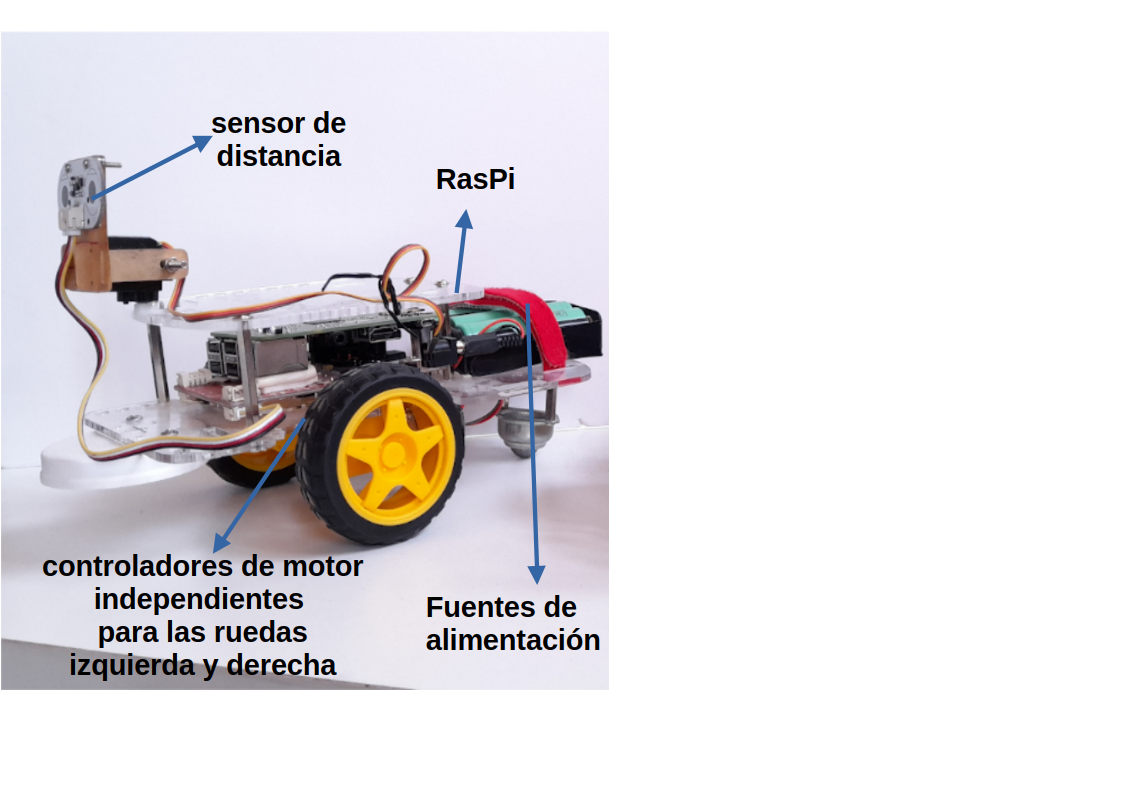
\includegraphics[width=\imsize]{robot_gopigo.png}
	\caption[Esquema del Robot GoPiGo de Dexter Industries, Mostrando Sensores de Distancia, Motores y Raspberry Pi Integrada, Utilizado en Conjunción con la Simulación del Connectoma de C. elegans.  ]{ Esquema del Robot GoPiGo de Dexter Industries, Mostrando Sensores de Distancia, Motores y Raspberry Pi Integrada, Utilizado en Conjunción con la Simulación del Connectoma de C. elegans.}\label{fig:robot}
\end{figure}



\subsection{Simulación de la dinámica neuronal en el connectoma de C. elegans}\label{sec:dinamica}

El robot sigue el diseño propuesto por Busbice, utilizando el connectoma de C. elegans (disponible en \url{https://github.com/openworm/}) para controlar un robot de dos ruedas. Para interactuar con el robot, se han creado dos módulos de Python: un módulo de entrada que lee los sensores del robot y estimula las neuronas apropiadas cuando se alcanzan umbrales específicos, y un módulo de salida que acumula estímulos de las neuronas motoras y, a su vez, envía la cantidad de potencia que se aplicará a cada uno de los dos motores. Estos dos módulos actúan como interfaces entre el robot y el connectoma.


\subsubsection{Modulo de entrada sensorial}

El robot utiliza un sensor de distancia GoPiGo para detectar obstáculos (\url{https://www.dexterindustries.com/store/distance-sensor/}). El sensor de distancia se ubica en la parte frontal del robot y se emplea para medir la distancia a los objetos en el camino del robot. Inicialmente, se utilizó un sensor ultrasónico estándar HC-SR04 para detectar obstáculos, pero se encontraron imprecisiones en las lecturas cuando el robot estaba en movimiento debido a que este tipo de sensor utiliza ondas de sonido para medir la distancia, y estas ondas pueden ser afectadas por el movimiento del robot. Por esta razón, se optó por cambiar al sensor GoPiGo Laser, el cual emplea el método de tiempo de vuelo para medir la distancia. Este método resulta mucho más preciso y no se ve afectado por el movimiento del robot. El proceso de detección de obstáculos funciona de la siguiente manera:


\begin{enumerate}
\item El sensor de distancia emite un pulso láser.
\item El pulso láser rebota en el obstáculo y regresa al sensor de distancia.
\item El sensor de distancia mide el tiempo que tarda el pulso láser en viajar de ida y vuelta.
\item Utilizando el tiempo de viaje, el sensor de distancia calcula la distancia al obstáculo.
\end{enumerate}


El sensor GoPiGo Laser ofrece varias ventajas sobre otros sensores de distancia basados en ultrasonido, incluyendo su precisión, velocidad y alcance. Puede medir la distancia de manera rápida y precisa, lo que lo convierte en una elección idónea para aplicaciones que requieren detección de obstáculos en tiempo real y con un alcance de hasta 5 metros, lo que resulta adecuado para situaciones en las que se necesita detectar obstáculos a distancia. Además de estas ventajas, el sensor GoPiGo Laser es fácil de instalar y usar, ya que se puede conectar a un puerto I2C en la placa Raspberry Pi y se puede utilizar con la biblioteca \textbf{DistanceSensor}. Las instrucciones detalladas sobre cómo conectar el sensor de distancia al robot se encuentran disponibles en \url{https://www.dexterindustries.com/GoPiGo/get-started-with-the-gopigo3-raspberry-pi-robot/}.


Basándonos en resultados de experimentos neurobiológicos y etológicos que demuestran que la nariz de C. elegans es una región altamente sensible, lo que lleva al nematodo a detenerse y cambiar de dirección cuando se encuentra con obstáculos (\Cref{sec:toquenariz}), decidimos utilizar el sensor mencionado para simular el sentido del tacto en la nariz del gusano. El sensor se activa cuando el robot se encuentra a menos de 30 centímetros de un objeto, una distancia que se ha comprobado ser efectiva. Las neuronas sensoriales estimuladas cuando el robot se encuentra a menos de 30 cm de un objeto son las siguientes: ASHL, ASHR, FLPL, FLPR, OLQDL, OLQDR, OLQVL, OLQVR, todas asociadas a este circuito sensorial.


\subsubsection{Detección de comida}

Detección de comida: Cuando el sensor de distancia no detecta obstáculos, estimulamos las neuronas quimiosensoriales responsables de la búsqueda de alimentos. Basándonos en resultados experimentales (\Cref{sec:quimiosensacion}) del comportamiento de búsqueda de alimentos, estimulamos las siguientes neuronas: ADFL, ADFR, ASGL, ASGR, ASIL, ASIR, ASJL, ASJR. En general, la estimulación de las neuronas sensoriales de alimentos activa el connectoma de manera más efectiva y hace que el robot comience a moverse hacia adelante.


 \subsubsection{Modulo de salida motora}
 
 
 Módulo de salida motora: El módulo de salida motora captura las salidas de las neuronas motoras y almacena los valores en una matriz en la que cada celda representa un músculo del cuerpo de C. elegans. Las neuronas motoras se conectan a los músculos para excitarlos o inhibirlos. El circuito neuromotor del gusano utiliza conexiones excitatorias e inhibidoras, lo que permite al gusano moverse de manera ondulante, contrayendo algunos músculos mientras relaja otros y viceversa. En total, hay 95 músculos corporales que recorren todo el cuerpo del gusano: 24 en la parte superior izquierda, 23 en la parte inferior izquierda, 24 en la parte superior derecha y 24 en la parte inferior derecha. Los músculos del cuerpo se dividen en izquierdos y derechos, y el valor acumulado se envía a los motores respectivos del robot. La velocidad máxima del motor se establece en 1000 DPS (grados por segundo), aunque este valor se suele reducir a 150 para evitar movimientos excesivamente rápidos en superficies lisas, aunque puede ajustarse en cualquier momento. Cuando el valor acumulado excede 150, el programa de salida lo restablece a 150. La relación entre los valores acumulados de los músculos izquierdos y derechos determina las señales que se envían a los motores del robot. La \Cref{fig:robot_2} muestra un diagrama de flujo que representa cómo se genera la salida motora.
 

 
  \begin{figure}[h!]
 	\centering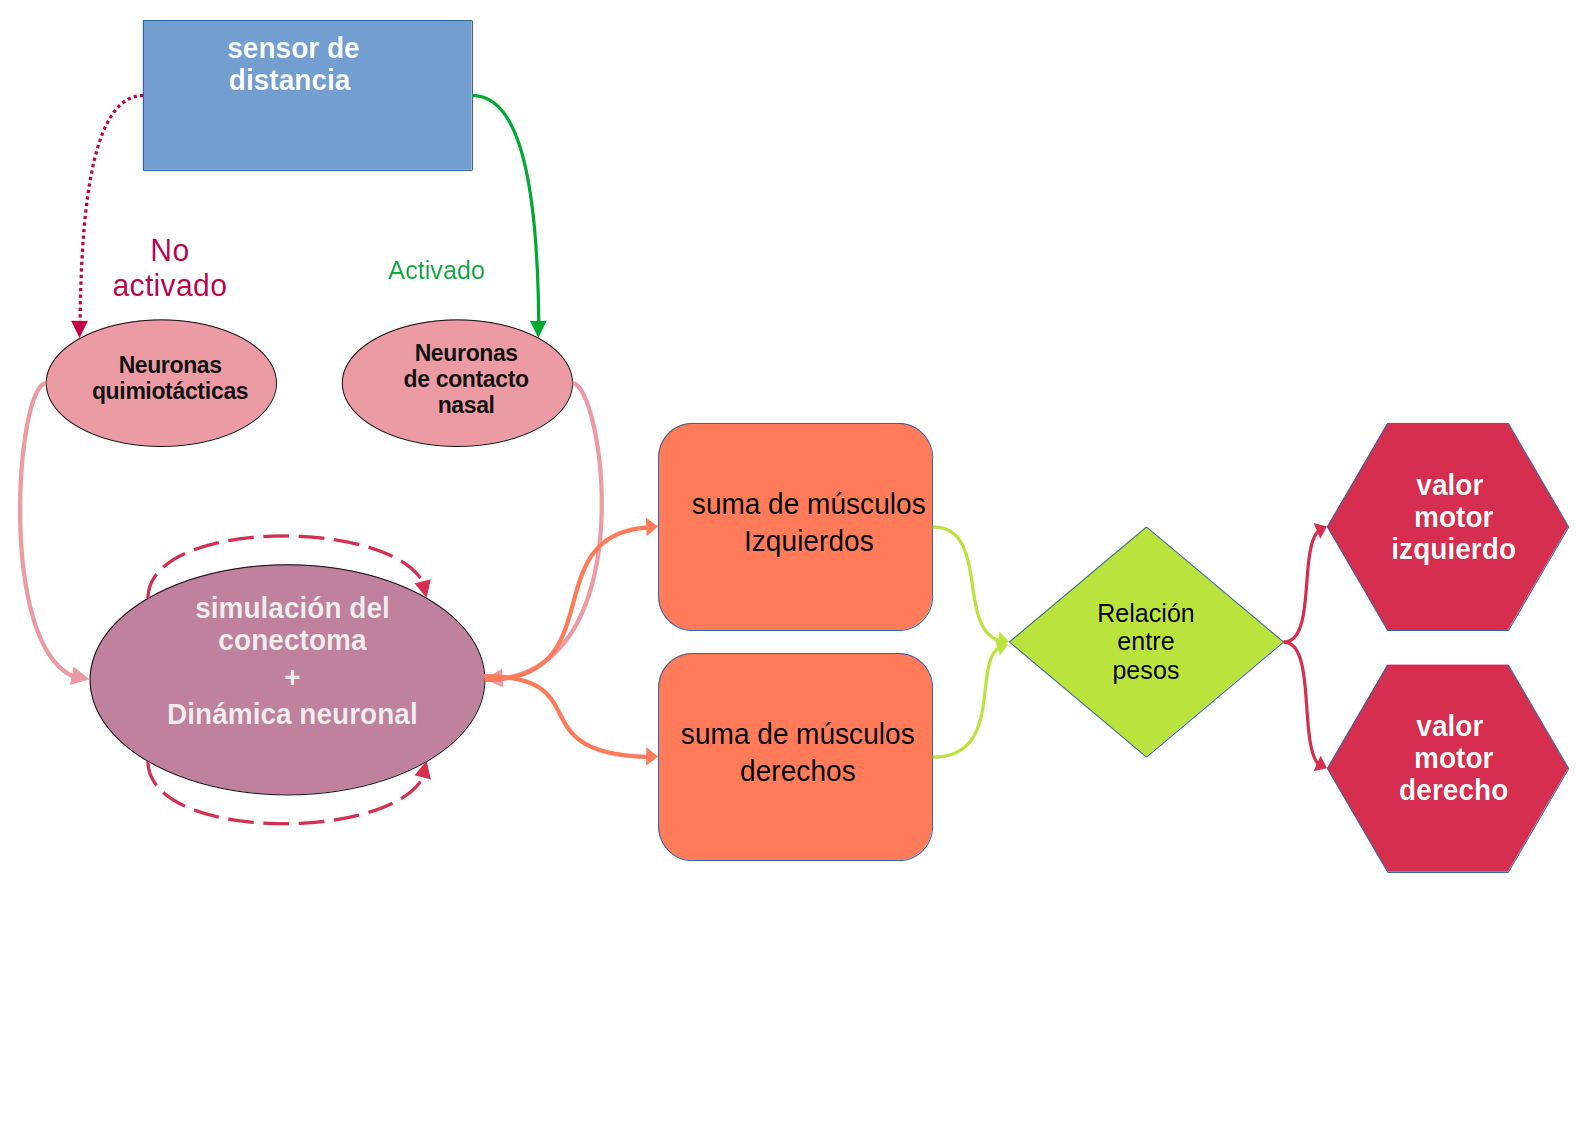
\includegraphics[width=\imsize]{robot_2.png}
 	\caption[Diagrama de Flujo que Ilustra la Generación de la Salida Motora.]{Diagrama de Flujo que Ilustra la Generación de la Salida Motora.}\label{fig:robot_2}
 \end{figure}
 

 
 
  \subsubsection{Modulo del conectoma}
 
El connectoma en sí se compone de un diccionario de Python con 300 entradas, cada una representando una neurona del connectoma de C. elegans (por ejemplo, AVAL, DB02 y VD03). Cada neurona está asociada a un diccionario que contiene las conexiones con otras neuronas, y el número de conexiones se utiliza como valor ponderado. Cuando una neurona dispara, se envía un valor ponderado a las neuronas conectadas. El programa principal se encarga de coordinar la simulación y controlar el robot.


 \subsection{Robot personalizado}

El robot personalizado sigue esencialmente los mismos pasos de construcción que el GoPiGo, pero en lugar de utilizar la placa GoPiGo 2 para el control de motores, emplea un controlador de motor dual L9110S (consulte las \Cref{fig:robot_personalizado,fig:robot_nuestro1,fig:robot_nuestro2}). En las \Cref{fig:sensor_distancia1,fig:sensor_distancia2} se muestra el diagrama de cableado del robot personalizado, que incluye la conexión del sensor de distancia directamente a la Raspberry Pi 3B y el cableado del controlador de motor L9110S.


\begin{figure}[h!]
	\centering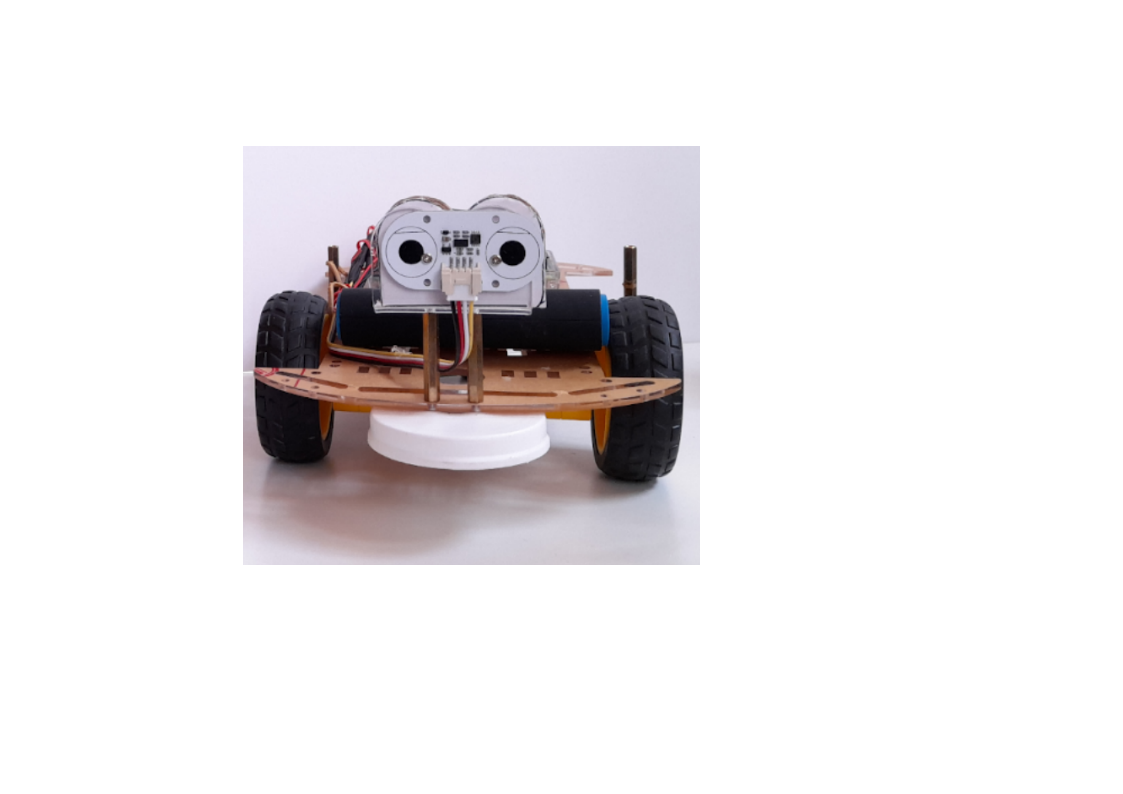
\includegraphics[width=\imsize]{robot_personalizado}
	\caption[Robot Personalizado Empleado en Nuestros Experimentos. ]{ Robot Personalizado Empleado en Nuestros Experimentos. Dado que el hardware del robot GoPiGo no es de código abierto, optamos por construir un robot personalizado, como se muestra a la derecha en la figura. En lugar de la placa GoPiGo 2, utilizamos un controlador de motor dual L9110S para el control de los motores. Este enfoque permite la construcción asequible del robot con componentes de fácil acceso y bajo costo.}\label{fig:robot_personalizado}
\end{figure}


\begin{figure}[h!]
	\centering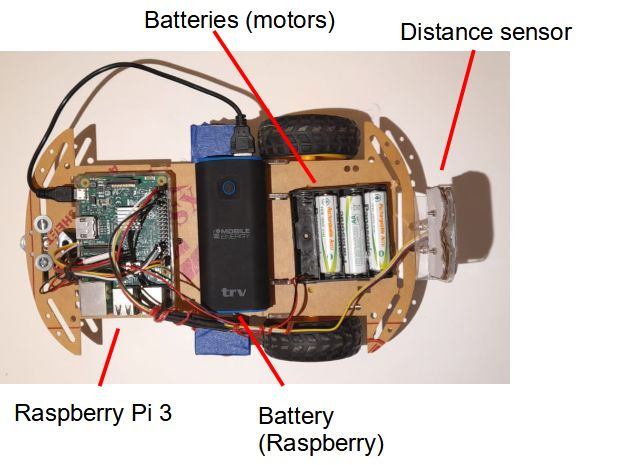
\includegraphics[width=\imsize]{robot_nuestro1.png}
	\caption[Vista Superior del Robot Personalizado.  ]{ Vista Superior del Robot Personalizado. En la imagen, se observa a la izquierda la Raspberry Pi, que ejecuta la simulación numérica para controlar el robot. La caja rectangular negra representa la batería que suministra energía a la Raspberry Pi, mientras que se emplea un paquete de baterías independiente para alimentar los motores. Además, se aprecia un sensor de distancia ubicado en la parte frontal del robot. }\label{fig:robot_nuestro1}
\end{figure}



\begin{figure}[h!]
	\centering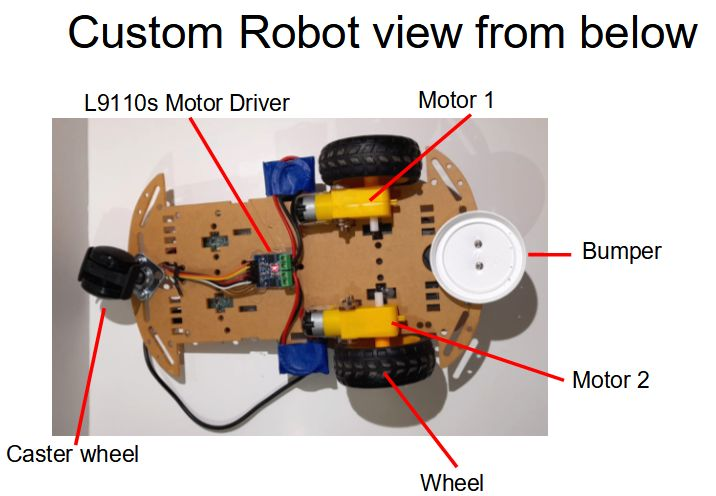
\includegraphics[width=\imsize]{robot_nuestro2.png}
	\caption[ Perspectiva Inferior del Robot Personalizado.]{ Perspectiva Inferior del Robot Personalizado. En esta vista, se aprecia la rueda giratoria a la izquierda, que proporciona soporte y facilita la maniobrabilidad del robot. En la parte inferior se encuentra el pequeño controlador de motores L9110s, permitiendo una conexión directa a los motores (en amarillo) que controlan las ruedas. Para proteger el sensor de distancia de posibles colisiones, se ha adjuntado un parachoques de goma en la parte delantera del vehículo.}\label{fig:robot_nuestro2}
\end{figure}


\begin{figure}[h!]
	\centering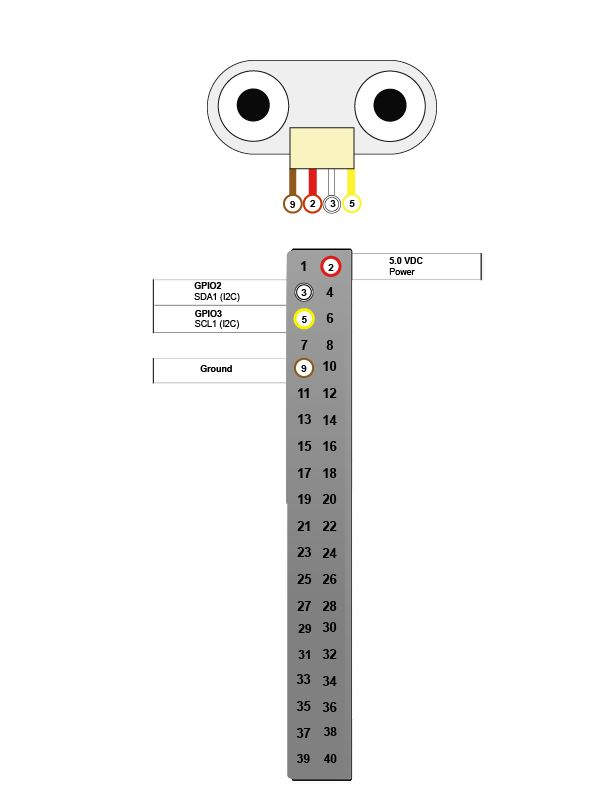
\includegraphics[width=\imsize]{sensor_distancia1.png}
	\caption[Conexión del Sensor de Distancia. ]{Conexión del Sensor de Distancia. En esta representación, se ilustra la conexión del sensor de distancia del GoPiGo directamente a los encabezados GPIO de una Raspberry Pi 3B en el robot personalizado. Las conexiones incluyen: Tierra (Ground), pin 9 (marrón), Alimentación (Power), pin 2 (rojo), SDA1 I2C, pin 3 (GPIO2, blanco) y SCL1 I2C, pin 5 (GPIO3, amarillo).}\label{fig:sensor_distancia1}
\end{figure}


\begin{figure}[h!]
	\centering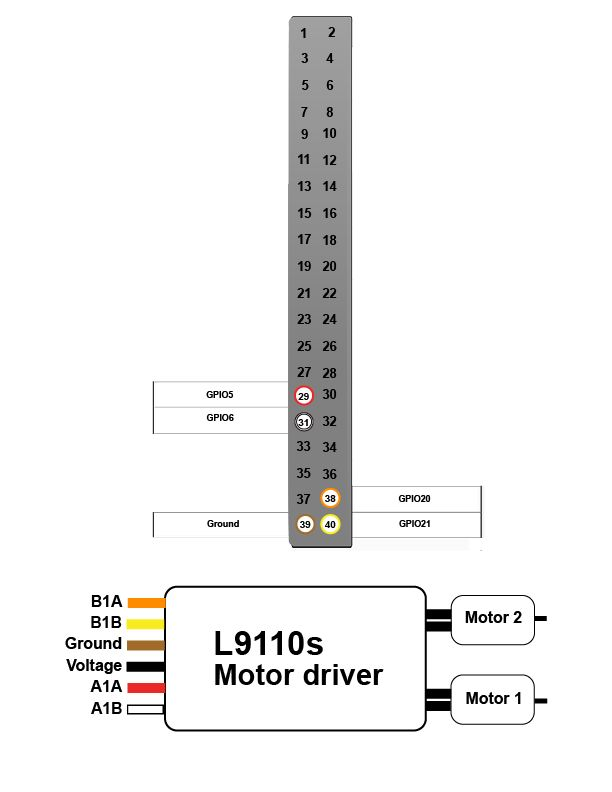
\includegraphics[width=\imsize]{sensor_distancia2.png}
	\caption[Conexión del Controlador de Motor.]{ Conexión del Controlador de Motor. En esta ilustración, se detalla cómo el controlador del motor L9110s se conecta a ambos motores y a los encabezados GPIO de una Raspberry Pi 3B en el robot personalizado. Las conexiones comprenden: B1A, pin 38 (GPIO20, naranja), B1B, pin 40 (GPIO21, amarillo), Tierra, pin 39 (marrón), Voltaje (conexión directa a la batería de 5V, negro), A1A, pin 29 (GPIO5, rojo) y A1B, pin 31 (GPIO6, blanco).}\label{fig:sensor_distancia2}
\end{figure}


\section{Dinámica neuronal global}\label{sec:dinamicakato}

Para explorar la dinámica global del robot que emula la actividad neuronal del C. elegans, hemos seguido la metodología propuesta por Kato et al. \cite{kato_global_2015}. En una primera etapa, calculamos las derivadas temporales de la actividad neuronal del robot. Para lograr esto, empleamos el método de diferenciación regularizada de variación total, cuyos detalles y justificaciones se encuentran en el \Cref{C:ap1}. La regularización desempeña un papel fundamental al reducir el ruido y la variabilidad en los datos, sin comprometer la información crítica.


Posteriormente, aplicamos el Análisis de Componentes Principales (PCA) a las derivadas temporales. Para este propósito, utilizamos la función de \textbf{PCA} de la biblioteca scikit-learn \footnote{https://scikit-learn.org/stable/modules/generated/sklearn.decomposition.PCA.html}. Esta técnica nos permitió no solo obtener los componentes principales (PC) ponderados de las neuronas, sino también calcular la varianza explicada por cada uno de estos componentes. Los PC se derivaron considerando la estructura de covarianza presente en los datos normalizados. Para una comprensión más completa de los PC, se recomienda la lectura de la referencia  \cite{noauthor_principal_2002}.

Con el objetivo de facilitar la interpretación de los resultados, aplicamos un filtro de promedio móvil a las trayectorias en el espacio de fases generadas mediante PCA. Este filtro consistió en un promedio de 10 muestras sucesivas. Paralelamente, generamos una serie de tiempo correspondiente a cada PC, denominada PC temporal. Esta serie se obtuvo mediante un promedio ponderado de las series temporales que abarcaban múltiples neuronas. Los PC temporales capturan señales compartidas por grupos de neuronas, que se agrupan en función de sus correlaciones.


Es importante destacar que realizamos el análisis PCA sobre las derivadas temporales de los datos, ya que los PC resultantes produjeron trayectorias en el espacio de estado que presentaban una organización espacial más coherente. Este enfoque nos brindó una visión más estructurada y representativa de la dinámica global del robot y su relación con el conectoma del C. elegans.



\section{Discusión}

En el marco de nuestra investigación, la elección de este diseño específico de robot se fundamenta en sus características intrínsecamente atractivas. La simplicidad en su construcción y su costo reducido lo destacan como una opción altamente replicable y económicamente eficiente en el contexto de la investigación científica. No obstante, la innovación reside en la simulación neuronal que rige el comportamiento del robot. Dicha simulación se basa en unidades dinámicas elementales e incorpora información biológica derivada del conectoma, lo que confiere al robot la capacidad de manifestar comportamientos emergentes, permitiéndole desenvolverse de manera autónoma y sortear obstáculos de forma natural.

Este modelo presenta una serie de distinciones clave en comparación con la mayoría de las simulaciones:

Primero, se trata de un modelo completo del conectoma, aunque es importante tener en cuenta que no se han incorporado todos los orgánulos o entradas sensoriales en el modelo en la etapa actual. Por ejemplo, los receptores de estiramiento, que podrían desempeñar un papel importante en los comportamientos de locomoción de C. elegans, aún no forman parte de este modelo en su estado actual de desarrollo.

Además, a diferencia de las simulaciones discretas, este modelo sigue una dinámica continua. La estimulación es constante y activa, imitando la operación de un sistema nervioso en tiempo real. Las modificaciones en la información sensorial tienen un impacto directo y continuo en el comportamiento del robot.

La naturaleza física del modelo también es una característica distintiva. El Connectome se encuentra conectado a un robot tridimensional real, lo que posibilita una interacción genuina con su entorno. Esta interacción es altamente impredecible y fundamental para la comprensión del comportamiento emergente.

En lo que respecta a la representación neuronal, cada neurona se modela mediante un programa individual, en analogía con el funcionamiento de las neuronas biológicas. Las entradas dendríticas y las salidas axonales solo responden a la cantidad de estimulación recibida por el programa correspondiente.

Dado que el Conectoma se representa mediante programas individuales, el tiempo de generación de la estimulación no es fijo, sino que varía según la evolución de los factores ambientales. El aspecto temporal es crucial, ya que la estimulación cambia a medida que los factores ambientales se modifican. Cada programa se configura para disparar su axón solo cuando se alcanzan ciertos umbrales, y con el tiempo, el programa se despolariza.

Sin embargo, a pesar de las ventajas mencionadas, hasta el momento no hemos realizado un análisis exhaustivo de la dinámica del modelo ni de su correlación con las acciones del robot. El capítulo siguiente se enfoca en presentar los resultados derivados de la aplicación de este modelo robótico al estudio del comportamiento motor emergente. Además, buscamos, en la medida de lo posible, comparar los resultados obtenidos en el robot con aquellos provenientes de experimentos recientes con C. elegans. Este enfoque nos brinda la oportunidad de adquirir una comprensión más profunda de la capacidad del modelo para simular con precisión el comportamiento del organismo biológico.












\chapter{Dinámica neuronal critica}\label{titulo-cap-critico}
\graphicspath{{figs/capitulo_critico/}}

\chapterquote{Can a machine be made to be supercritical? }{Alan Turing , 1950}






\section{Introducción}

La física de sistemas complejos ha demostrado que los comportamientos colectivos pueden surgir de la interacción entre los constituyentes elementales de la materia, dando lugar a fases con diferentes niveles de orden interno. Los sistemas biológicos no son la excepción, y algunos de ellos han sido identificados como operando en la vecindad del punto crítico de una transición de fase. En este sentido, la hipótesis de la criticidad neuronal sugiere que el cerebro puede estar en un estado crítico en el límite entre diferentes tipos de dinámicas, lo que le proporcionaría un equilibrio óptimo entre robustez y flexibilidad.

En este capítulo se revisarán las bases teóricas de la física de sistemas complejos y su aplicación en biología, así como los fundamentos de la hipótesis de la criticidad neuronal y las evidencias experimentales que la respaldan.






\section{Física de sistemas complejos y transiciones de fase}

\subsection{Transiciones de fase en física}

La materia, compuesta por átomos, moléculas y electrones, puede generar diversas fases cuyo comportamiento difiere significativamente de sus componentes individuales o pequeños grupos de ellos. A nivel microscópico, los sistemas que contienen muchos componentes pueden exhibir diferentes tipos de comportamientos colectivos a nivel macroscópico, es decir, fases, con diferentes niveles de orden interno. Es importante destacar que incluso pequeños cambios en las condiciones externas, como la temperatura o la presión, pueden inducir reordenamientos estructurales drásticos, lo que se conoce como transiciones de fase.\\

En la distinción de las distintas fases de un sistema, se consideran ciertas propiedades macroscópicas medibles, conocidas como parámetros de orden. La variación de una propiedad ambiental, denominada parámetro de control, permite observar cómo dichos parámetros de orden cambian. En general, una modificación gradual en el parámetro de control se traduce en una alteración suave en los parámetros de orden. Sin embargo, existen determinados puntos donde los valores de los parámetros de orden experimentan saltos o giros abruptos (ver \Cref{fig:trancisiones}). Estos puntos marcan los límites entre diferentes fases, y desplazar el parámetro de control a través de dicho límite induce una transición de fase.\\

En función de cómo se modifiquen los parámetros de orden durante una transición de fase, esta puede ser de dos tipos. Si la transición se caracteriza por un salto en los parámetros de orden del sistema, lo que matemáticamente corresponde a una discontinuidad en el diagrama de fase, se trata de una transición de fase discontinua (ver \Cref{fig:transicionI} ). Este tipo de transiciones son denominadas a veces como transiciones de primer orden. Por otra parte, si el diagrama de fase es continuo y la transición se caracteriza por una esquina aguda (es decir, un punto de no diferenciabilidad), se trata de una transición de fase continua (segundo orden, ver \Cref{fig:transicionII}). La terminología de \textquote{primer orden} y \textquote{segundo orden} se origina en la descripción de las transiciones de fase termodinámicas, haciendo referencia a la derivada más baja de la energía libre, la cual muestra una discontinuidad en el punto crítico.\\


\begin{figure}[ht]
	\centering
	\begin{subfigure}[b]{0.45\textwidth}
		\centering
		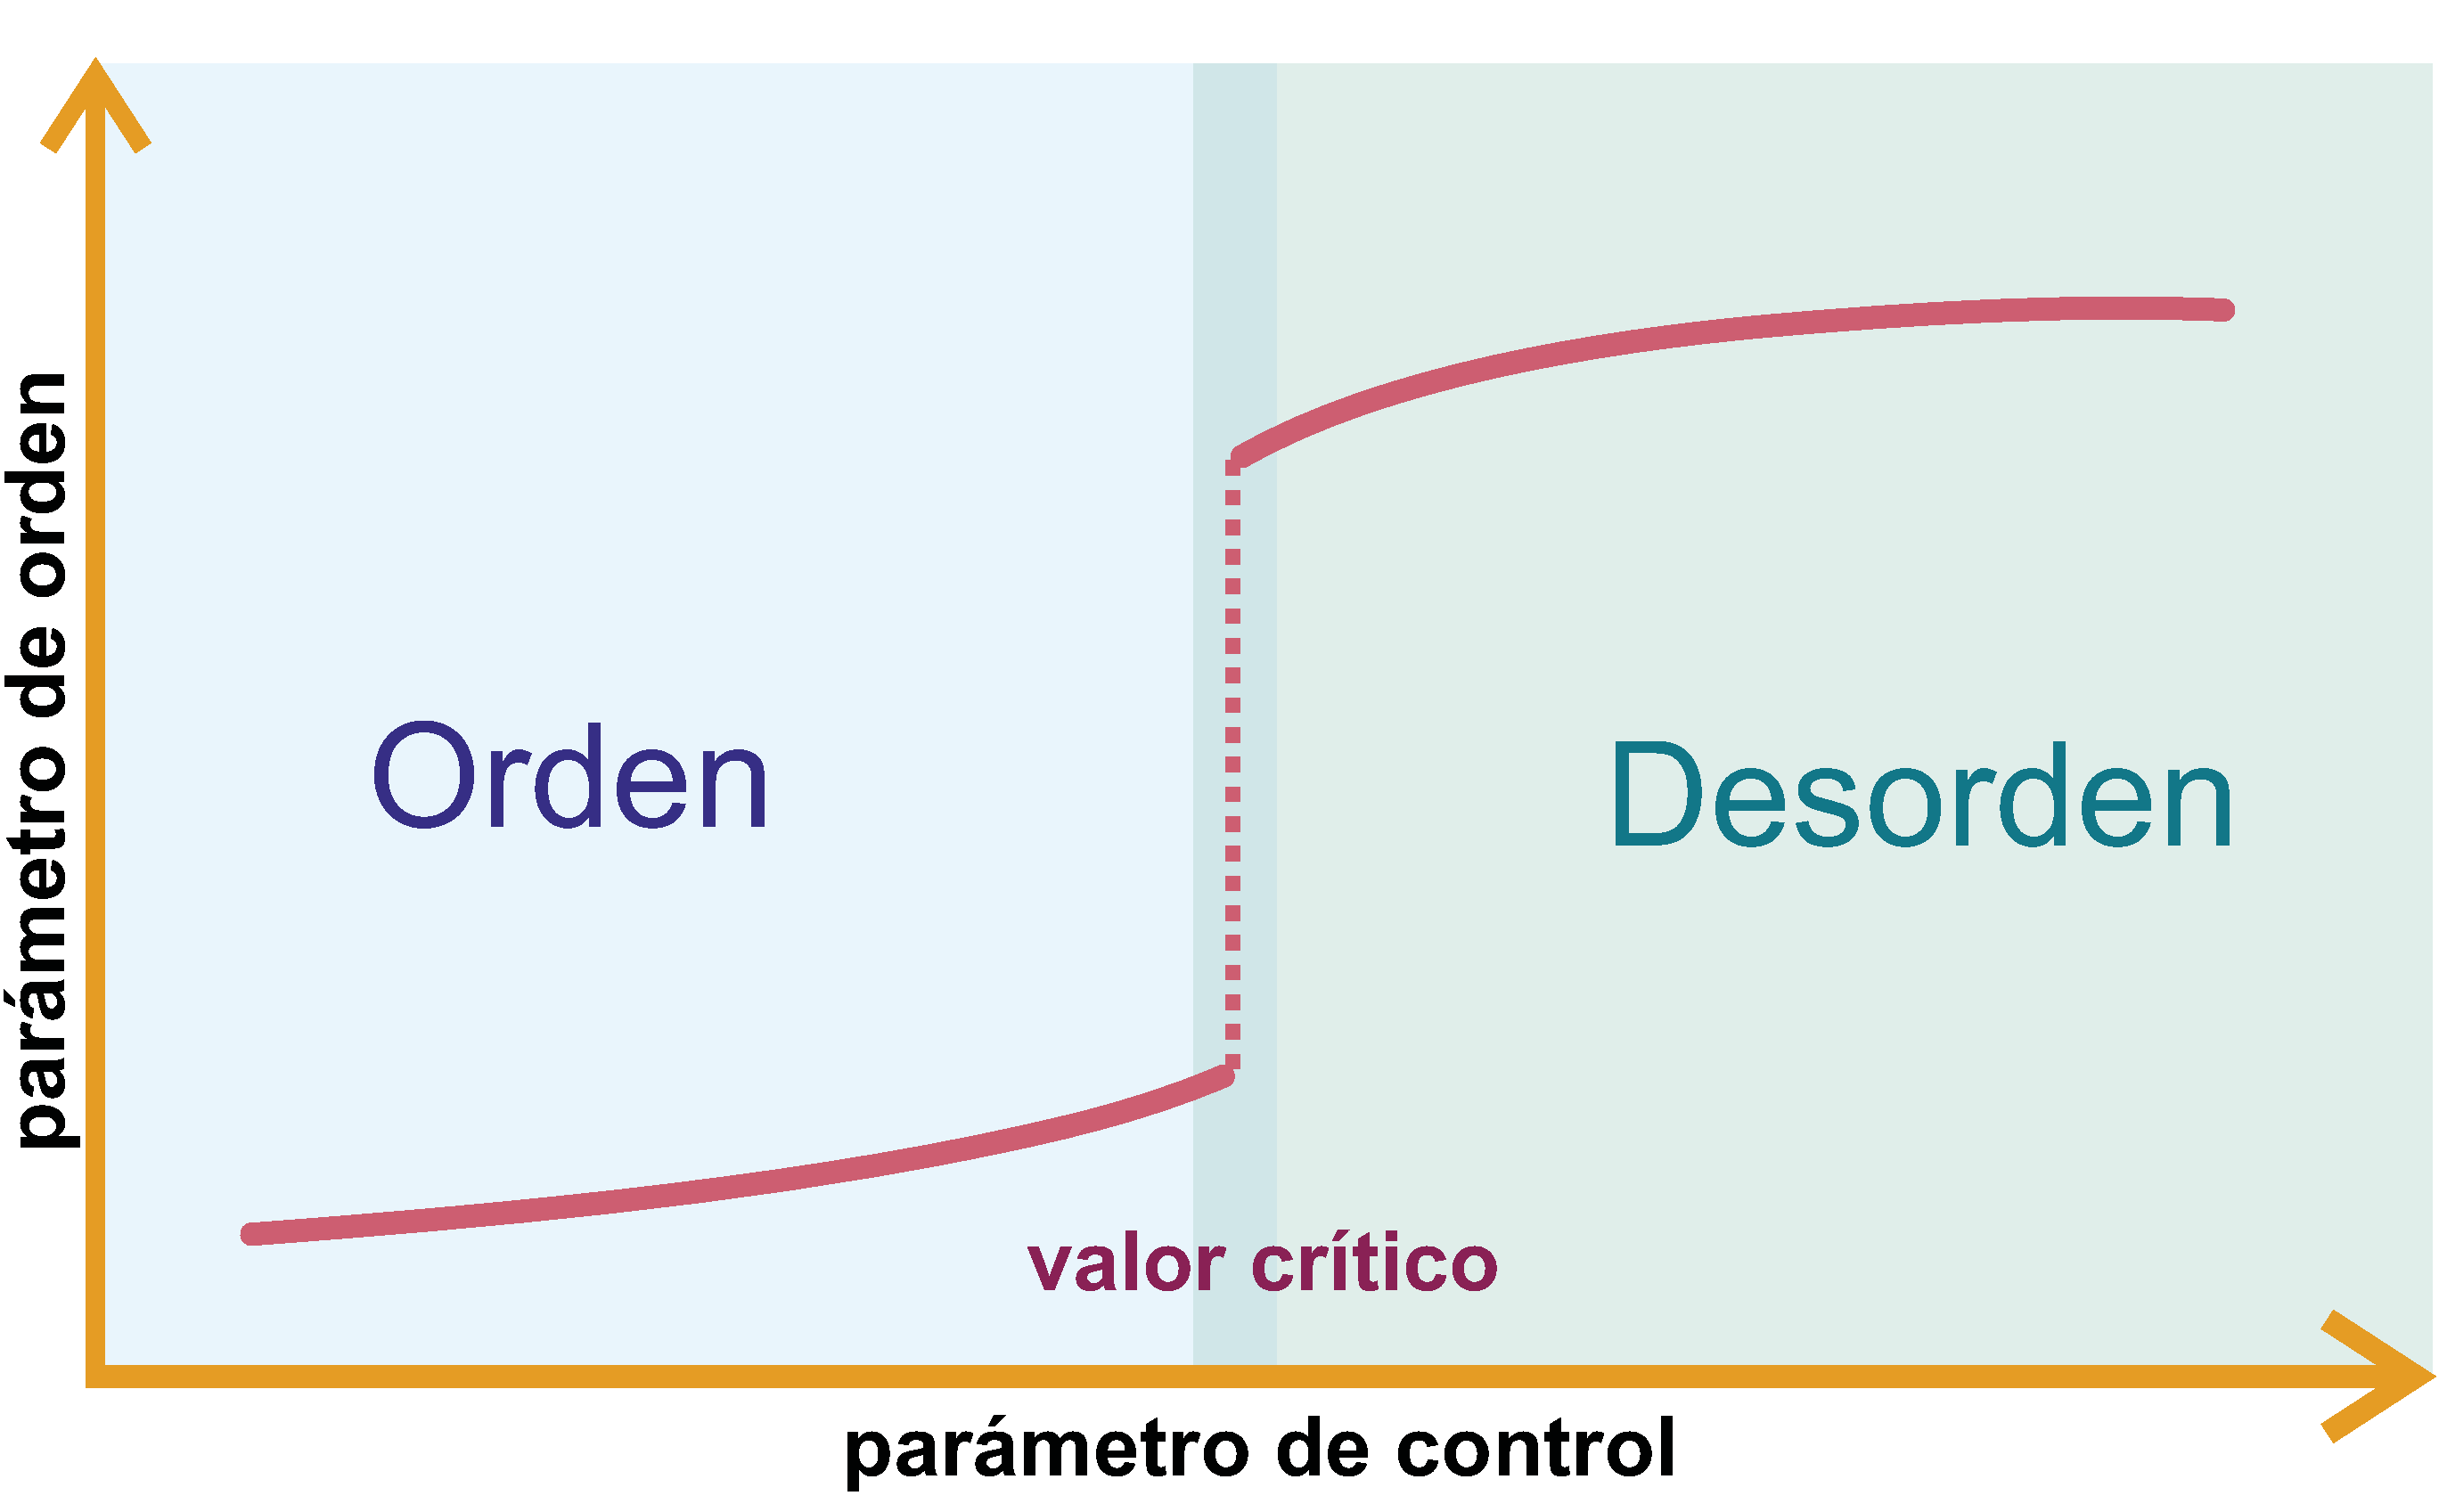
\includegraphics[width=\textwidth]{transiciones_fases_tipo_I.pdf}
		%\caption{transiciones de fase de primer orden}
		\caption{}
		\label{fig:transicionI}
	\end{subfigure}
	\begin{subfigure}[b]{0.45\textwidth}
		\centering
		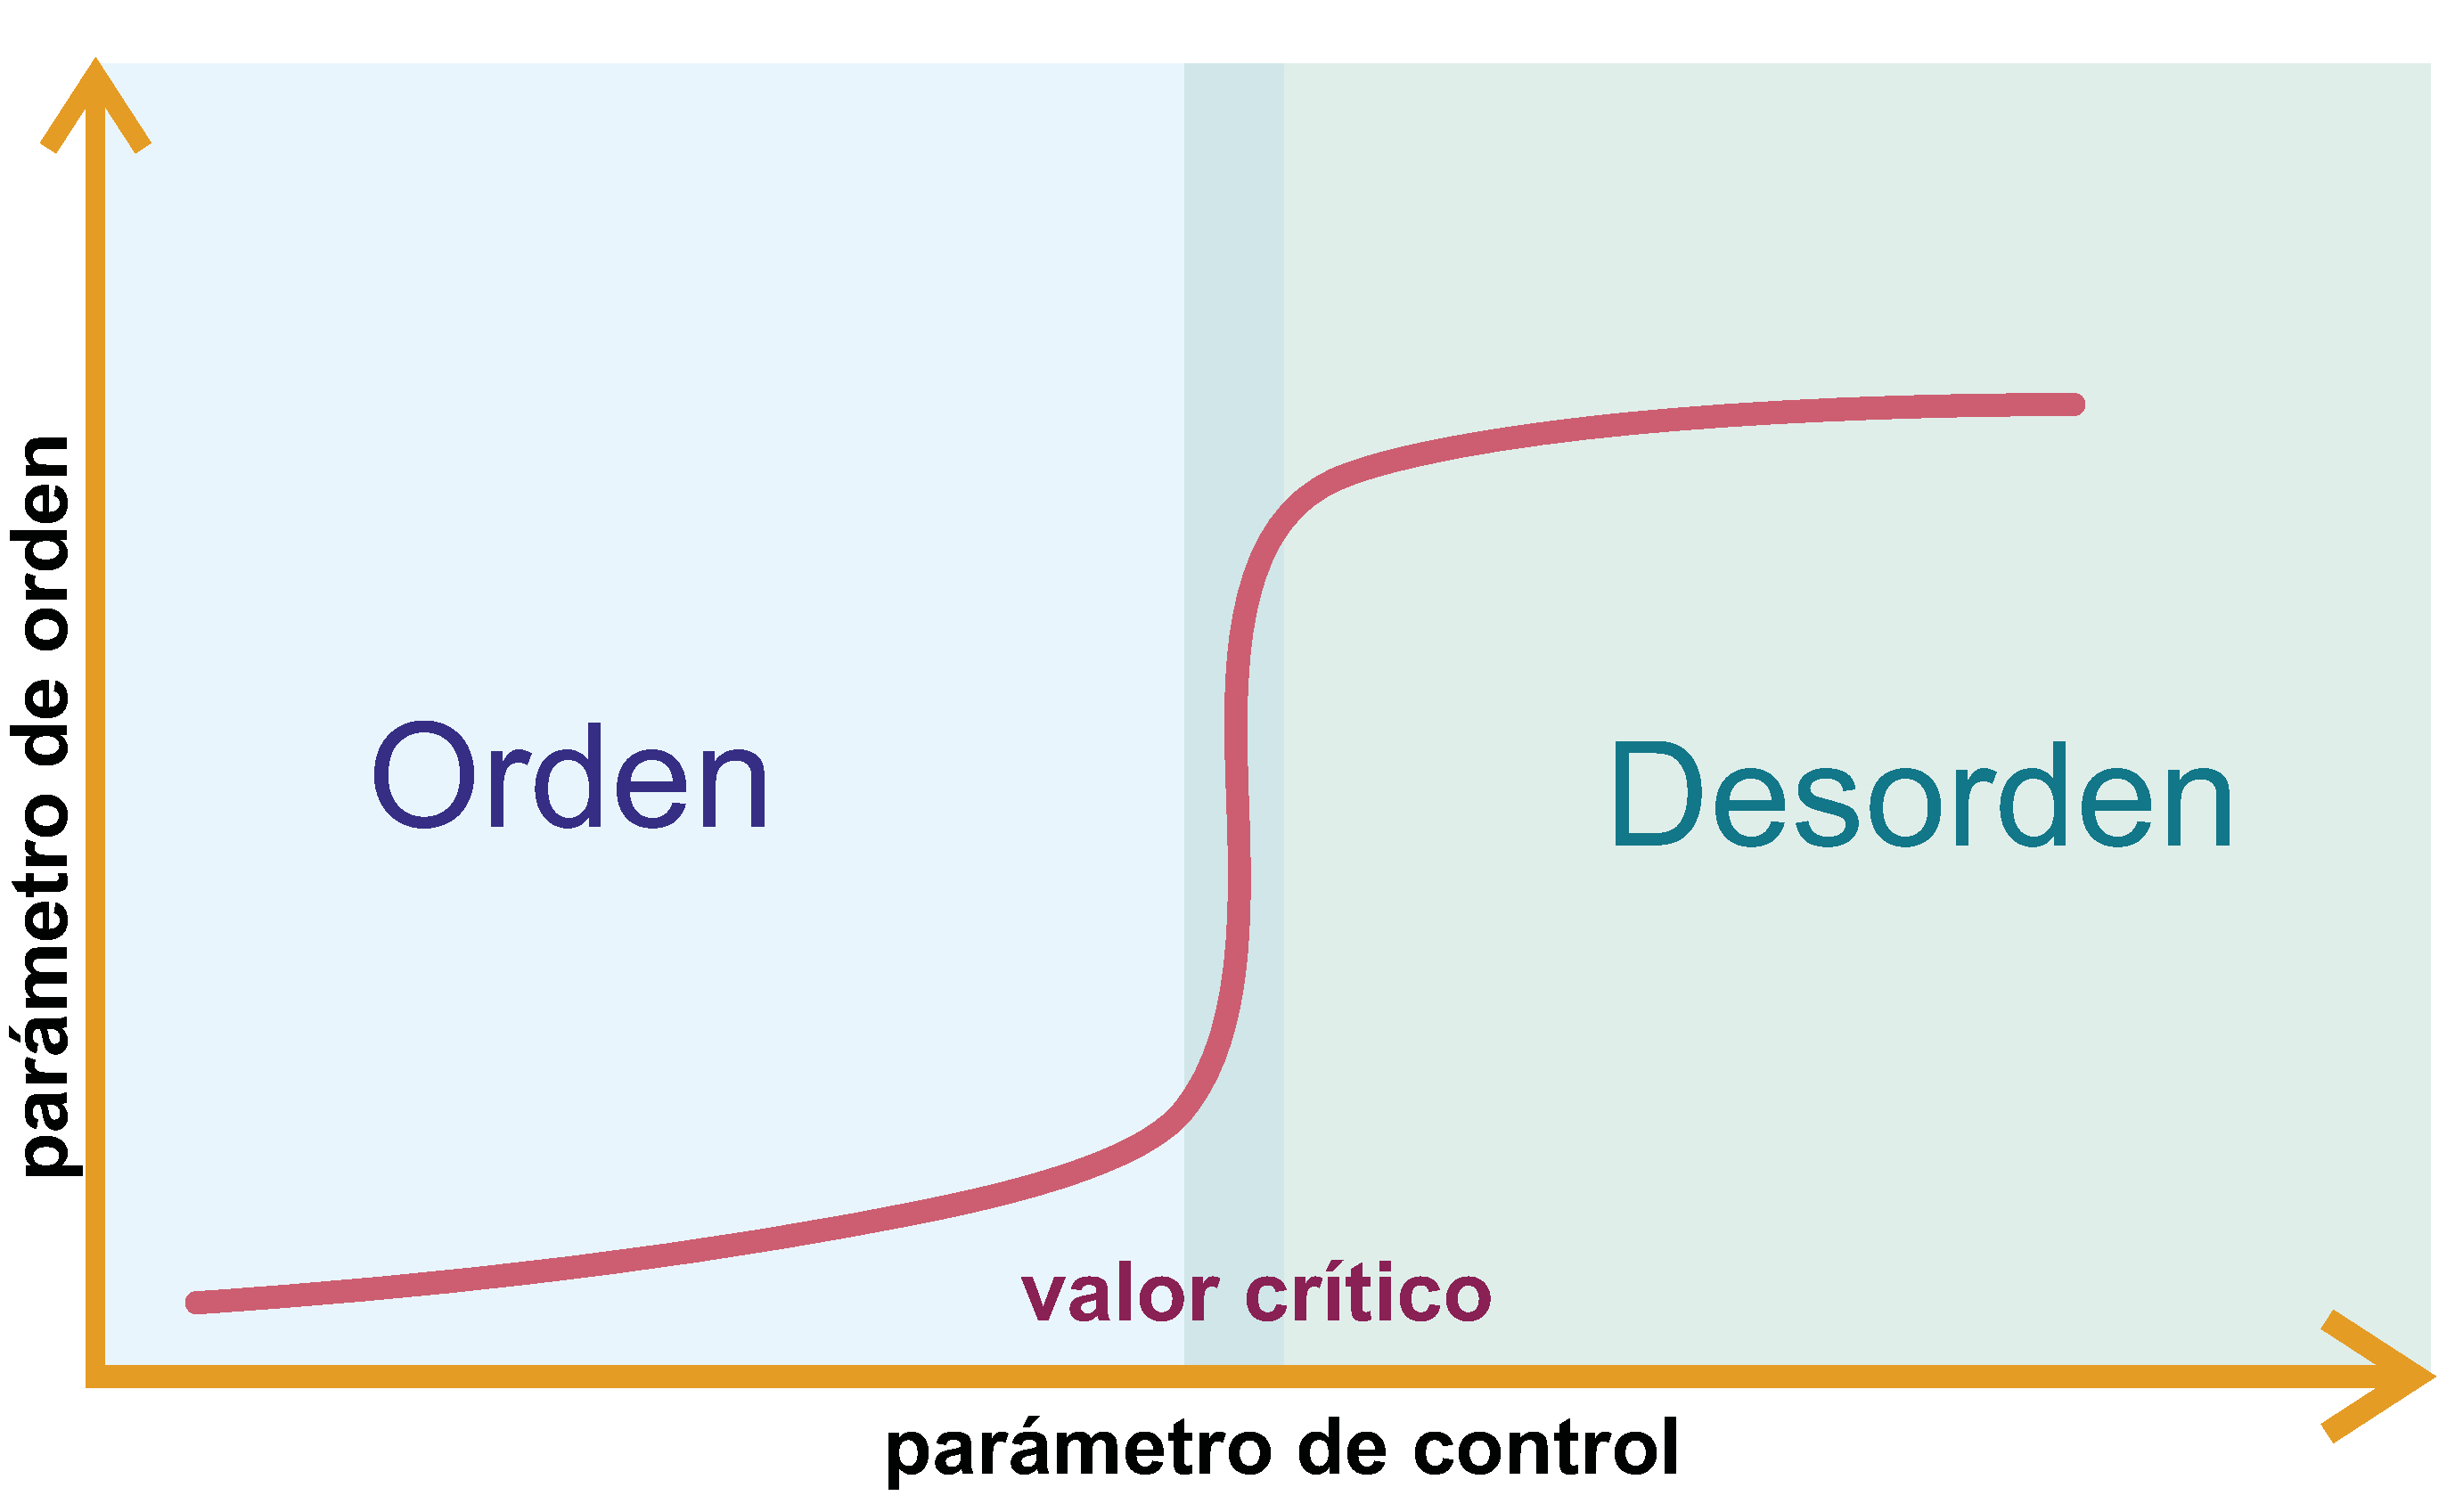
\includegraphics[width=\textwidth]{transiciones_fases_tipo_II.pdf}
		%\caption{transiciones de fase de segundo orden}
		\caption{}
		\label{fig:transicionII}
	\end{subfigure}
	\caption[Representaciones esquemáticas de transiciones de fase de primer y segundo orden.]{Representaciones esquemáticas de transiciones de fase de primer y segundo orden. La figura muestra dos ejemplos de transiciones de fase que ocurren en sistemas termodinámicos. En (a), se ilustra una transición de fase de primer orden, donde el parámetro de orden experimenta un cambio abrupto en su valor crítico del parámetro de control. En contraste, en (b) se muestra una transición de fase de segundo orden, donde el parámetro de orden varía suavemente a medida que cambia el parámetro de control.}
	\label{fig:trancisiones}
\end{figure}

Si un sistema exhibe una transición de fase continua, entonces puede existir en un punto crítico que se encuentra exactamente en la frontera entre dos fases distintas. Este estado límite, conocido como estado crítico, se caracteriza por la presencia de fluctuaciones importantes en el valor del parámetro de orden en el rango crítico, lo cual refleja la pérdida de simetría del sistema que ocurre durante las transiciones de fase. Por consiguiente, se considera que los estados críticos se encuentran en la frontera del caos. Las transiciones de fase críticas son especialmente interesantes debido al comportamiento crítico que se manifiesta en las grandes fluctuaciones del parámetro de orden, las cuales exhiben escalamiento de ley de potencia (Figura 1C).\\



\subsection{Transiciones de fase en biología}


El principio de universalidad es un concepto ampliamente aceptado en la física que establece que las características relevantes de los fenómenos a gran escala son altamente insensibles a los detalles específicos del modelo y se comparten entre sistemas aparentemente distintos. Siguiendo este principio, se ha propuesto una hipótesis controvertida, pero ampliamente investigada, según la cual algunos sistemas biológicos pueden obtener beneficios funcionales significativos al operar cerca del punto crítico de una transición de fase \cite{munoz_colloquium_2018,hidalgo_information-based_2014,kauffman_origins_1993,bak_how_1996,chialvo_brain_2008,chialvo_emergent_2010,plenz_critical_2013,niebur_criticality_2014,shew_functional_2013,cocchi_criticality_2017,zimmern_why_2020}. En particular, estos sistemas operarían en el límite entre una fase activa o caótica, en la que las fluctuaciones son amplificadas y la información se corrompe, y una fase inactiva u ordenada, en la que las fluctuaciones se amortiguan rápidamente y se reduce la capacidad de respuesta y adaptación. Se han identificado varios ejemplos de tales transiciones, como se resume en el \cref{table:transiciones_biologicas}.\\



% primer estilo 
%row{odd} = {bg=azure8},
%row{1} = {bg=azure3, fg=white, font=\sffamily},

% segundo estilo 

%row{odd} = {bg=red8},
%row{even} = {bg=red9},
%row{1} = {bg=red3, fg=white, font=\sffamily}

% tercer estilo 

%row{odd} = {bg=gray8},
%row{even} = {bg=gray9},
%row{1} = {bg=red3, fg=white, font=\sffamily},

%otra 

%row{odd} = {bg=teal9},
%row{1} = {bg=teal3, fg=white, font=\sffamily},
\begin{table}[h!]
	\centering
		\caption[Ejemplos seleccionados de transiciones de fase en biología.]{ Ejemplos seleccionados de transiciones de fase en biología, adaptado de Heffern et al\protect{\cite{heffern_phase_2021}}.}
\begin{tblr}{colspec={X[2,l]X[2,l]X[2,l]X[l]},
row{odd} = {bg=gray8},
row{even} = {bg=gray9},
row{1} = {bg=red3, fg=white, font=\sffamily},
}
	sistema	& parámetro de control	  &   parámetro de orden	& referencias seleccionadas
	  \\
	
	Fusión de la membrana plasmática	 & Temperatura	  &  Fluidez &    \cite{de_kruyff_effect_1972} \\
	

	Sincronización neuronal	 &   Fuerza sináptica; relación de excitación a inhibición	 &  Sincronización de tasas de disparo	 &    \cite{adhikari_time-delay-induced_2011,baumgarten_critical_2019}\\
	
	{Agrupamiento\\/enjambre}	 & Densidad; ruido en la percepción del comportamiento de los vecinos	  & Alineación de patrones de vuelo	  &   \cite{cavagna_scale-free_2010,bahar_flocking_2018,attanasi_finite-size_2014}  \\
	
	Rigidez de actina	 &   Densidad	 &   Rigidez &   \cite{gurmessa_triggered_2019,hussain_spatiotemporal_2013}  \\
	
Colapso de la población microbiana	 	&  Nivel de estrés	 & Crecimiento  &  \cite{mensonides_metabolic_2002,ordway_phase_2020}  \\
	
	Evolución cultural	 &  Cambios en el \gls{fitness} acompañado de \gls{epistasis} entre rasgos culturales	 &  Paradigma cultural	 & \cite{pascual_epistasis_2020}    \\
	
	
Rasgos del fitoplancton	 	& Condiciones de luz	  &   Contenido de clorofila	&  \cite{held_second-order_2020}  \\
	
	Colapso de la población de megafauna	 &   Variado& Tamaño de la poblacion	  &  \cite{hein_population_2019,lauerburg_socio-ecological_2020,heinze_quiet_2021}   \\
	
	Percolación de rigidez en embriogénesis de pez cebra	 &  Conectividad celular dependiente de la adhesión	 & Viscosidad del tejido, tamaño del grupo	  &  \cite{petridou_rigidity_2021}   \\
	
	\end{tblr}
	\label{table:transiciones_biologicas}
\end{table}

Existen varios experimentos que respaldan esta hipótesis. Algunos de estos ejemplos incluyen las transiciones de fase de sincronización en osciladores biológicos colectivos, como los relojes circadianos \cite{garcia-ojalvo_modeling_2004}; las transiciones de percolación de fibras en tejidos conectivos, como el colágeno \cite{forgacs_phase_1991,newman_phase_2004,alvarado_molecular_2013}; la transición de fase de fusión en hebras de ADN \cite{magee_jr_theory_1963,li_phase_2006}; las transiciones entre diferentes regímenes dinámicos, como las oscilaciones y los estallidos, en redes neuronales \cite{kelso_phase_1984,freeman_metastability_2005,rabinovich_dynamical_2006,werner_metastability_2007,adamatzky_chaos_2013,haken_principles_1996}; los patrones de expresión génica \cite{tsuchiya_self-organizing_2016};  el agrupamiento bacteriano \cite{larkin_signal_2018,ordway_phase_2020}  y la formación de colonias de C. elegans \cite{chen_c_2021}. Para obtener una revisión más completa de las aplicaciones de las transiciones de fase a problemas biológicos, se recomienda consultar la obra de Heffern et al \cite{heffern_phase_2021}.\\





\section{Hipótesis de la criticidad neuronal}
En línea con lo anteriormente expuesto, la hipótesis de la criticidad neuronal sostiene que el cerebro de los organismos puede estar en un estado crítico en el límite entre diferentes tipos de dinámicas \cite{hesse_self-organized_2014}.  De manera similar a lo que ocurre en los sistemas biológicos, se ha argumentado que la criticidad proporciona a los sistemas neuronales un equilibrio óptimo entre robustez frente a las perturbaciones y flexibilidad para adaptarse a condiciones cambiantes, así como para conferirles capacidades computacionales óptimas \cite{legenstein_edge_2007,tagliazucchi_signatures_2017}, amplios repertorios dinámicos \cite{shew_neuronal_2009}, gran estabilidad de la red \cite{bertschinger_real-time_2004}, transmisión y almacenamiento óptimo de la información \cite{plenz_organizing_2007,beggs_criticality_2007,haldeman_critical_2005,lombardi_balance_2012,vazquez-rodriguez_stochastic_2017}, máxima sensibilidad a los estímulos \cite{kinouchi_optimal_2006,liu_plasticity_2015}  y un comportamiento global coordinado \cite{schneidman_weak_2006,beggs_neuronal_2003}.\\

Numerosos modelos específicos, como redes booleanas \cite{kauffman_emergent_1984,derrida_random_1986}, máquinas de estado líquido \cite{langton_computation_1990}, redes neuronales y redes de filtración de nanopartículas de plata \cite{carstens_brain-like_2022} , han verificado esta hipótesis (ver también Haykin et al \cite{haykin_what_2007} para una revisión). \\

Experimentalmente, se ha evidenciado que los sistemas neuronales parecen mostrar características de los sistemas en estado crítico, lo que sugiere que la hipótesis de la criticidad neuronal podría ser una explicación plausible para la dinámica del cerebro. Estos estudios incluyen:

\begin{itemize}
\item Invariancia de escala de las avalanchas neuronales \cite{fontenele_criticality_2019,beggs_neuronal_2003,beggs_neuronal_2004}  reportadas en diversas especies \cite{hahn_neuronal_2010,petermann_spontaneous_2009,shriki_neuronal_2013}, a través de diferentes técnicas de imagen \cite{tagliazucchi_criticality_2012} y señales electrofisiológicas \cite{linkenkaer-hansen_long-range_2001}. Al igual que en los sistemas biológicos, se ha encontrado que los sistemas neuronales exhiben una dinámica que es independiente de la escala temporal y espacial, lo que sugiere que los procesos neuronales son más similares a los procesos de los sistemas complejos en estado crítico que a los procesos aleatorios o regulares.
\item La presencia de correlaciones espacio-temporales de largo alcance en las fluctuaciones de amplitud de las oscilaciones neuronales \cite{expert_self-similar_2010,fraiman_what_2012,kitzbichler_broadband_2009}, incluida la observación de espectros de potencia $1/f$ de señales \acrshort{MEG}/\acrshort{EEG} registradas simultáneamente \cite{linkenkaer-hansen_long-range_2001}, resonancia magnética funcional  \cite{kitzbichler_broadband_2009} y respuestas cognitivas  \cite{van_orden_human_2005,shew_adaptation_2015}. Estas correlaciones sugieren que los sistemas neuronales exhiben una dinámica compleja y a largo plazo, lo que es consistente con la dinámica en estado crítico.
\item El aumento de la longitud de correlación con el tamaño del sistema \cite{fraiman_what_2012,ribeiro_trial-by-trial_2022,haimovici_brain_2013}. Al igual que en los sistemas biológicos, los sistemas neuronales parecen ser más estables y tener una dinámica más compleja a medida que aumenta el número de componentes.
\end{itemize}




\subsection{Mecanismos homeostáticos de mantenimiento  del estado Crítico}

Es posible conjeturar que la criticidad emerge en los sistemas vivos como resultado de procesos adaptativos y evolutivos que sirven como una plantilla para una mayor complejidad. Esta hipótesis propone que la criticidad podría ser una estrategia organizativa común en biología derivada de la física de las transiciones de fase. Sin embargo, aún hay muchas preguntas sin respuesta sobre la hipótesis de la criticidad.\\

Una de las principales preguntas es cómo un sistema complejo como el cerebro puede permanecer sintonizado en un estado crítico. Es importante tener en cuenta que la teoría de las transiciones de fase normalmente considera sistemas infinitos, mientras que en sistemas grandes pero finitos, las transiciones de fase se suavizan en un pequeño rango de parámetros. En lugar del punto crítico singular, encontramos una pequeña región que no es técnicamente crítica, pero que aún conserva muchas propiedades de criticidad \cite{moretti_griffiths_2013}. Sin embargo, incluso permanecer en esta región \textquote{crítica}  debería requerir mecanismos que resintonicen activamente el cerebro. La idea general de sistemas que se ajustan a estados críticos a través de procesos descentralizados activos se conoce como criticidad autoorganizada (\gls{soc}, por sus siglas en inglés) \cite{bak_how_1996,christensen_evolution_1998,bornholdt_topological_2000,bornholdt_self-organized_2003}.\\

El término \gls{soc}  describe las propiedades de los sistemas fuera del equilibrio para alcanzar un estado estacionario caracterizado por correlaciones de largo alcance, que se asemejan a las transiciones de fase de segundo orden cerca del equilibrio. En tales casos, el sistema desarrolla una respuesta multiescala que gradualmente alcanza un estado metaestable con correlaciones espaciales y temporales de largo alcance sin un parámetro de ajuste obvio o una transición de fase (dinámica). Por lo tanto, los estados del  \gls{soc} aparecen como un atractor de la dinámica no lineal en un sistema abierto repetidamente impulsado por fuerzas externas (o endógenas) \cite{tadic_self-organised_2021,gross_adaptive_2007}. \\

Sin embargo, los sistemas nerviosos son sistemas no conservativos en contraste con los sistemas \gls{soc}  canónicos como los modelos de pilas de arena \cite{jensen_self-organized_1998,pruessner_self-organised_2012}. Para modelar tales sistemas, se utilizan redes no conservativas de elementos representados por autómatas celulares, mapas de tiempo discretos o ecuaciones diferenciales. Dichos modelos tienen características distintas de los sistemas conservadores. Una gran parte de ellos, en particular las redes neuronales, muestran \gls{SOqC} \cite{bonachela_self-organization_2009,bonachela_self-organization_2010,buendia_feedback_2020} o criticidad débil \cite{palmieri_emergence_2018,palmieri_forest_2020}. Con el tiempo, varios autores propusieron diferentes mecanismos biológicos que podrían eliminar el ajuste fino y convertir a la región crítica en un atractor autoorganizado \cite{kinouchi_mechanisms_2020,zeraati_self-organization_2021,meisel_adaptive_2009,droste_analytical_2013,tetzlaff_self-organized_2010,meisel_failure_2012,rocha_homeostatic_2018,plenz_self-organized_2021,levina_phase_2009,ma_cortical_2019}. La criticidad obtenida no es perfecta, pero es suficiente para dar cuenta de los datos experimentales. Además, los mecanismos (principalmente basados en sinapsis dinámicas, pero también en ganancias neuronales dinámicas, regulación homeostática de la inhibición y umbrales de activación adaptativos) son biológicamente plausibles y deben considerarse como un tema de investigación por derecho propio.


\section{Trastornos cerebrales y alteraciones de la criticidad}


En las anteriores secciones se ha examinado la relación de la criticidad con un comportamiento óptimo de la dinámica cerebral y los mecanismos que la organizan y mantienen. Se ha planteado la hipótesis de que las propiedades dinámicas que caracterizan un estado crítico pueden verse como un marcador importante del bienestar cerebral. En este sentido, las desviaciones de la criticidad pueden ser sintomáticas o causales de ciertas patologías, lo que allana el camino para nuevos diagnósticos y tratamientos.\\

A pesar del creciente interés en la criticidad biológica en las últimas dos décadas, ha habido una escasez de estudios experimentales y clínicos que conecten la criticidad con las perturbaciones. Debido a que la criticidad representa un estado óptimo para el cerebro, se esperaría que la salida del estado crítico suponga una interrupción en sí misma \cite{heiney_criticality_2021}. Sin embargo, en la práctica, las interrupciones en la dinámica de la red probablemente sean más complicadas que una transición fuera de la criticidad, ya que dichas transiciones pueden ser parte de una actividad saludable.\\

Es importante destacar que existen aplicaciones clínicas de estos hallazgos en varios trastornos neurológicos, como la epilepsia \cite{osorio_epileptic_2010,witton_rogue_2019,kramer_human_2012,moosavi_criticality_2023,meisel_antiepileptic_2020}, las enfermedades neurodegenerativas como la enfermedad de Alzheimer \cite{stam_disturbed_2005,montez_altered_2009,vysata_change_2014} y la enfermedad de Parkinson \cite{hohlefeld_long-range_2012,herrojo_ruiz_long-range_2014,west_parkinsonian_2016}, derrames cerebrales \cite{rocha_recovery_2022}, así como otros dominios clínicamente relevantes, como la anestesia \cite{alonso_dynamical_2014,thiery_long-range_2018,liu_scale-free_2014}, la medicina del sueño \cite{bocaccio_avalanche-like_2019} (incluyendo el insomnio \cite{meisel_decline_2017,colombo_more_2016}, la apnea del sueño \cite{lo_asymmetry_2013} y la narcolepsia), neurodesarrollo \cite{padilla_breakdown_2020,smit_scale-free_2011,mares_age-dependent_2013}, la cognición, atención, aprendizaje y autismo \cite{ezaki_closer_2020,jia_attenuation_2018,ouyang_decomposing_2020,tinker_power_2014,dimitriadis_altered_2013}, efectos psicológicos del neurofeedback y los psicodélicos \cite{zhigalov_modulation_2016,tagliazucchi_enhanced_2014}, las afecciones psiquiátricas comunes como la depresión \cite{gartner_aberrant_2017}, la esquizofrenia \cite{moran_long-range_2019}, la ansiedad \cite{tolkunov_power_2010} y el trastorno de estrés postraumático \cite{ros_tuning_2014}.  Se dispone de una revisión muy completa de estos temas en el artículo escrito por Vincent Zimmern \cite{zimmern_why_2020}.\\

No obstante, a pesar de los avances en la investigación, todavía no se ha incorporado la criticidad en la práctica clínica habitual. Esto se debe en parte a la falta de estudios experimentales y clínicos que conecten la criticidad con las perturbaciones, y también a la necesidad de formación de equipos multidisciplinarios en los que los físicos, matemáticos, científicos de datos y médicos colaboren para responder mejor a una pregunta clínica a través de la lente de la criticidad.\\

En este contexto, se espera que el futuro de la criticidad en el ámbito clínico dependa en gran medida de la formación de estos equipos multidisciplinarios y de la aplicación de técnicas de análisis cuantitativo de electroencefalografía (\gls{EEG}), \glossary{MEG} y resonancia magnética funcional (\gls{fMRI}), entre otras. De esta forma, podrían desarrollarse nuevas herramientas diagnósticas y terapéuticas que permitan una mejor comprensión y tratamiento de diversas enfermedades neurológicas y psiquiátricas.



\section{Métricas experimentales de criticidad}



En las secciones anteriores se ha presentado la hipótesis de criticidad y su relevancia en los sistemas biológicos, así como sus limitaciones y aplicaciones. En esta sección, se aborda la detección de las transiciones de fase y la dinámica crítica en experimentos y simulaciones.
La construcción de un diagrama de fase es la evidencia más directa de una transición de fase (ver \Cref{fig:trancisiones} ) \cite{dickman_paths_2000}. En este tipo de diagrama, se puede observar la respuesta del parámetro de orden ante las variaciones del parámetro de control, lo que permite detectar la existencia de una transición de fase. Sin embargo, la construcción de dicho diagrama requiere que el parámetro de control sea accesible y controlable en el entorno experimental, lo que puede resultar difícil en sistemas biológicos complejos.\\

Por ejemplo, la variación de la conectividad cerebral in vivo puede ser difícil de lograr experimentalmente. Debido a estas limitaciones, la mayor parte de la evidencia de la criticidad en sistemas biológicos proviene de la observación de características distintivas en los resultados experimentales. En esta sección, se discuten las características distintivas de la criticidad que se han identificado en la literatura científica y que se utilizan para establecer la presencia de criticidad en sistemas biológicos \cite{hesse_self-organized_2014}. Estas características distintivas son fundamentales para la identificación de la dinámica crítica en sistemas biológicos complejos, especialmente aquellos cuya dinámica interna es imposible o difícil  de modificar.



\subsection{Escalamiento de la ley de potencia}


En el ámbito de la estadística, una variable aleatoria continua $X$ se considera que tiene una distribución de ley de potencia cuando se extrae de una distribución de probabilidad con densidad $	\mathbb{P}\left(x\leq X\leq x+dx\right)=Cx^{-\alpha}dx$. El parámetro $\alpha$ se conoce como el exponente o parámetro de escala, mientras que $C$ es un parámetro de normalización. Por otro lado, una variable aleatoria discreta de ley de potencia tiene una versión discretizada similar de la probabilidad, que se puede expresar como 	$P(X=k)=Ck^{-\alpha}$.\\

Es importante señalar que en la práctica, son pocos los fenómenos empíricos que obedecen leyes de potencia para todos los valores de $X$. En general, las leyes de potencia se utilizan para caracterizar la cola de la distribución, es decir, la distribución de probabilidad de los valores de $X$ mayores que algún valor $x_{min}$. En estos casos, se dice que la cola de la distribución sigue una ley de potencia. Además, los datos a menudo muestran una distribución de ley de potencia truncada, lo que significa que el comportamiento de ley de potencia solo se observa en un rango limitado, $x_{min}\leq X \leq x_{max}$  \cite{touboul_can_2010}.\\

Cabe destacar que las leyes de potencia presentan invariancia de escala, lo que las convierte en distribuciones libres de escala. Una función $f(x)$ se considera invariante de escala si $ f(cx)  = \left(cx\right)^{-\alpha}=c^{-\alpha}x^{-\alpha}=c^{-\alpha}f(x)\propto f(x)$, lo que indica que escalar el argumento de la función es equivalente a escalar proporcionalmente la función misma. Además, como $\log(p(x))=\log_{\alpha}\left(ax^{-\alpha}\right) = -\alpha\log(x)+\log(a)$, el histograma de la ley de potencias presenta una relación afín en un gráfico logarítmico (\Cref{fig:leypotencia}).\\

Debido a esto, las leyes de potencia en datos empíricos se suelen analizar graficando el logaritmo del histograma en función del logaritmo de los valores de la variable aleatoria. Luego, se aplica un algoritmo de mínimos cuadrados para ajustar una línea afín a través de los puntos de datos. Este método se remonta a Pareto en el siglo XIX \cite{arnold_pareto_2008}. Sin embargo, es importante destacar que la inspección visual de un diagrama puede generar falsos positivos. Además, se ha señalado que las pruebas convencionales de bondad de ajuste no son adecuadas para las leyes de potencia \cite{newman_power_2005}.\\



\begin{figure}[ht]
	\centering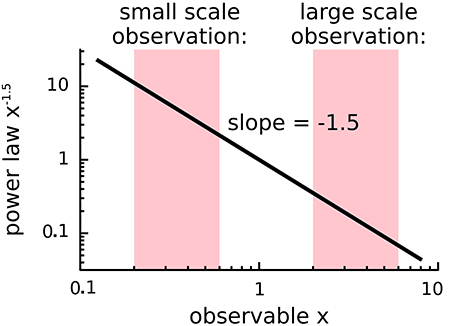
\includegraphics[width=\imsize]{fnsys-08-00166-g003.jpg}
	\caption[Representación gráfica de la independencia de escala de las leyes de potencia en una distribución de datos.]{Representación gráfica de la independencia de escala de las leyes de potencia en una distribución de datos, donde se ha utilizado la ley de potencia $f(x) = x^{-\alpha}$  con un exponente crítico de $\alpha=-1.5$ y una escala logarítmica en el eje $x$. La figura muestra que, independientemente del rango o escala utilizada para medir la distribución, se observa una ley de potencia con el mismo exponente crítico.} 	\label{fig:leypotencia}
\end{figure}


La hipótesis de criticidad en experimentos y simulaciones se basa en la presencia de leyes de potencia, que se espera se manifiesten en la mayoría de los sistemas críticos. Sin embargo, la existencia de leyes de potencia por sí sola no es suficiente para probar la criticidad \cite{goldstein_problems_2004,priesemann_can_2018}, ya que estas leyes también pueden ser explicadas por mecanismos no críticos \cite{touboul_can_2010,markovic_power_2014,noauthor_critical_2006,beggs_being_2012}. Por tanto, la identificación de leyes de potencia es un asunto delicado que requiere procedimientos de ajuste avanzados, debido a la dificultad para diferenciarlas de otras distribuciones de colas pesadas.\\

Las distribuciones de cola pesada son aquellas distribuciones de probabilidad cuyas colas son \textquote{más pesadas} que la distribución exponencial, siendo la gaussiana un subtipo de esta última. Entre los ejemplos de distribuciones de cola pesada se encuentran la distribución de Fisher-Tippett (doble exponencial), la distribución logarítmica normal y la distribución de Weibull, entre otras. Aunque se espera la presencia de leyes de potencia en sistemas críticos, estas distribuciones también pueden presentarse en otros sistemas no críticos. Por ende, para una mejor comprensión de la relevancia de las distribuciones de cola pesada en la neurociencia, se sugiere consultar la obra de Roberts et al  \cite{roberts_heavy_2015}.\\

Para abordar esta problemática, los investigadores han tenido acceso a metodologías estadísticas más sofisticadas gracias a los trabajos realizados por Clauset et al  \cite{clauset_power-law_2009} y otros estudios posteriores \cite{klaus_statistical_2011,markovic_power_2014}. Estas metodologías permiten distinguir las leyes de potencia de otras distribuciones de colas pesadas y evaluar su presencia en sistemas críticos. Sin embargo, es importante tener en cuenta que las leyes de potencia se truncan en sistemas de tamaño finito \cite{bonachela_self-organization_2010} y pueden verse afectadas por el submuestreo \cite{ribeiro_undersampled_2014}. Por lo tanto, es necesario emplear medidas cuantitativas para evaluar la diferencia entre las distribuciones de probabilidad acumulada experimental y ajustada por ejemplo  a través del parámetro $\kappa$ \cite{shew_neuronal_2009}.



\subsection{Escalamiento de  la ley de potencia de las avalanchas neuronales }

Beggs y Plenz demostraron experimentalmente que el comportamiento espontáneo de las redes corticales in vitro exhibe características consistentes con dinámicas críticas en su estudio histórico sobre avalanchas neuronales en cortes corticales interconectados con arreglos de microelectrodos (\gls{MEA}) \cite{beggs_neuronal_2003} . Una avalancha neuronal es una duración de actividad persistente que se propaga a través de la red y está marcada por períodos de silencio que preceden y siguen al período activo (ver \Cref{fig:avalancha}). En el caso de sistemas in vitro (es decir, cortes o cultivos disociados), la \textquote{actividad } puede referirse a los picos de mayor frecuencia o el \gls{LFP} de menor frecuencia, ya que se han estudiado ambas modalidades.\\

\begin{figure}[ht]
	\centering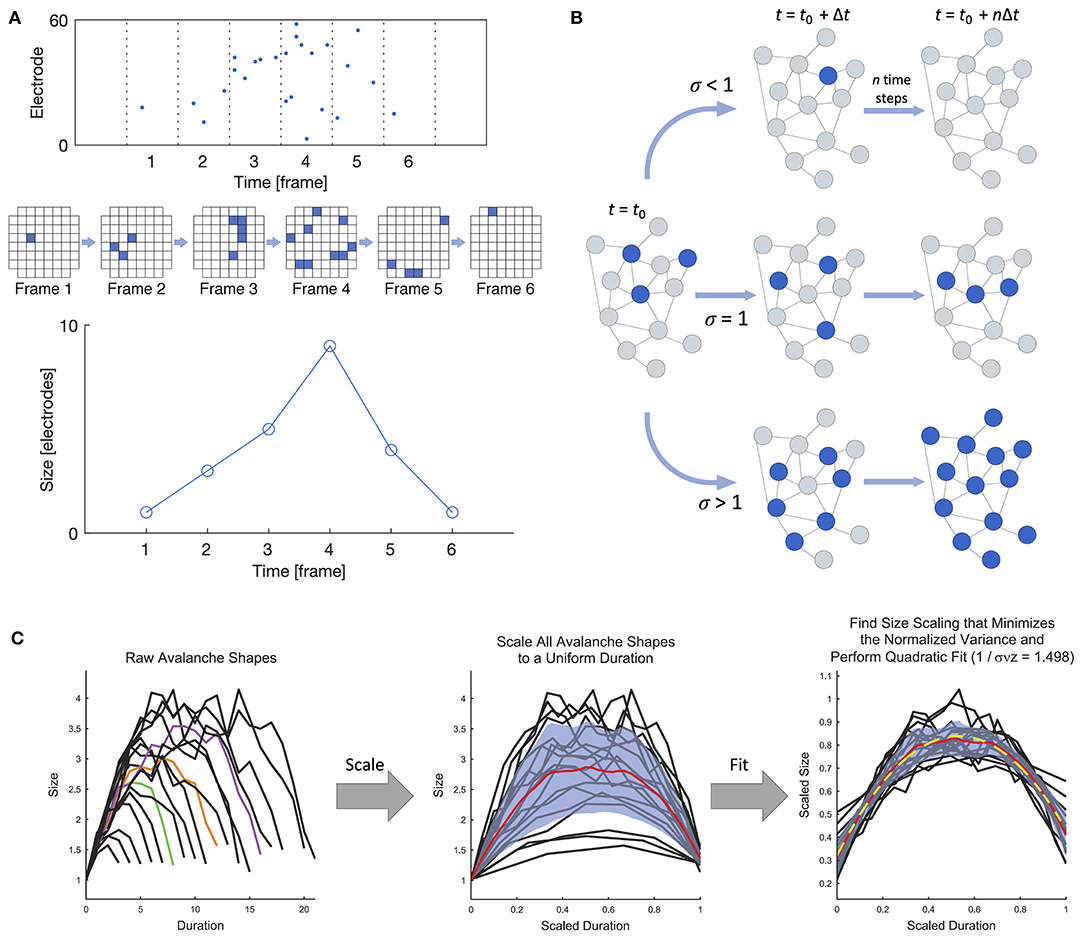
\includegraphics[width=\imsize]{fncom-15-611183-g002.jpg}
	\caption[Definición de avalancha neuronal y ejemplos de medidas empíricas de criticidad. ]{Definición de avalancha neuronal y ejemplos de medidas empíricas de criticidad. 
		(a) Se presenta la definición de avalancha neuronal, mostrando en el panel superior un gráfico rasterizado dividido en intervalos de tiempo. La avalancha representada abarca seis fotogramas activos, precedidos y seguidos por fotogramas inactivos. A continuación, se muestra una vista alternativa de la actividad en los seis marcos, en la que cada cuadrado representa un electrodo activo en una cuadrícula de 8x8. El panel inferior exhibe la definición de la forma de avalancha, la cual se obtiene a partir del número de electrodos activos en cada cuadro.
		(b) Se ilustra la relación de ramificación, en la cual los nodos azules representan actividad activa y los grises, inactiva. En una relación de ramificación de 1, la actividad persiste sin sobrecargar el sistema.
		(c) Se observa el colapso de forma en un sistema crítico, donde todas las avalanchas deberían mostrar el mismo perfil de forma temporal media en diferentes escalas de tamaño.
		Esta representación ha sido adaptada de Heiney et al.  \protect{\cite{heiney_criticality_2021}}.} 	\label{fig:avalancha}
\end{figure}


El escalamiento de la ley de potencia del tamaño $S$ y la duración $T$ de las avalanchas neuronales es un sello distintivo de la criticidad en las redes neuronales. Es decir, $P(S) \propto S^{-\alpha}$  y $P(T) \propto T^{-\beta}$, donde $P(·)$  es la función de distribución de probabilidad. El tamaño se define generalmente como el número de electrodos o neuronas activados, y la duración es el número de intervalos de tiempo activos. Los exponentes de la ley de potencia del tamaño y la duración son aproximadamente $\alpha=1.5$ y $\beta= 2.0$, respectivamente, cuando se selecciona el ancho del intervalo de tiempo para que se corresponda con el intervalo promedio entre picos. Sin embargo, la escala de la ley de potencia debe persistir en un rango de resoluciones temporales cercano al orden de magnitud del intervalo promedio entre picos, con el exponente $\alpha$ cambiando sistemáticamente con el tamaño del intervalo de tiempo seleccionado \cite{beggs_neuronal_2003,pasquale_self-organization_2008}. La escala de ley de potencia también debe mantenerse cuando se considera una resolución espacial de grano más grueso, utilizando solo un subconjunto de todos los puntos de registro. Las redes neuronales pueden mostrar varios puntos críticos dinámicos únicos, de los cuales solo uno es la transición de fase que da lugar a las avalanchas neuronales. Por lo tanto, es crucial considerar el contexto más amplio y no limitarse a la transición de fase en sí misma \cite{kanders_avalanche_2017}.







\subsection{Parámetro de ramificación}



En la teoría de los procesos de ramificación \cite{harris_theory_1963} se utiliza una medida común, la relación de ramificación $\sigma$, para evaluar el número de descendientes y ancestros en un sistema. En particular, esta medida establece la proporción entre el número de descendientes y el número de ancestros, en el que la actividad en un electrodo o neurona ancestro precede inmediatamente a la actividad en un electrodo o neurona descendiente \cite{beggs_neuronal_2003}. En un sistema en estado crítico, la relación de ramificación se aproxima a $1$, lo que permite que la actividad fluya a través de la red sin extinguirse ($\sigma < 1$) o saturar toda la red ($\sigma > 1$), tal como se muestra en la \cref{fig:avalancha}. Por tanto, la presencia de una relación de ramificación $\sigma = 1$ en respuesta a una excitación artificial en un sistema lo suficientemente inactivo puede considerarse como una evidencia de criticidad.\\

No obstante, es importante destacar que, en comparación con otras características, la evidencia proporcionada por una relación de ramificación de uno es relativamente débil. Esto se debe a que dicha relación no implica necesariamente una dinámica crítica, ya que también puede ser observada en estados supercríticos \cite{hesse_self-organized_2014}. Por lo tanto, se requiere de un análisis más riguroso que permita distinguir entre ambos estados.


\subsection{Colapso de forma}


La dinámica de los sistemas críticos se caracteriza por la presencia de avalanchas de actividad, que exhiben una naturaleza autosimilar o fractal. Se espera que la \textquote{forma} de la actividad de la avalancha se comporte como un fractal en dichos sistemas. En un estado crítico, se espera que todas las avalanchas muestren el mismo perfil temporal medio en todas las escalas. El perfil temporal de una avalancha se define como el número de sitios activos en función del tiempo. Para un sistema en estado crítico, los perfiles temporales de todas las avalanchas colapsan en la misma forma de perfil cuando se escala espacio-temporalmente con un exponente de escala$\gamma$ cercano a $2$(\Cref{fig:avalancha}). Esta propiedad se describe por  $ \left\langle S\right\rangle(T) \propto T^{-\gamma}$, donde $\left\langle S\right\rangle(T)$  representa el tamaño promedio de todas las avalanchas de una duración determinada $T$.\\

Se puede encontrar información detallada sobre el colapso de la forma en la literatura científica, como en Sethna et al \cite{sethna_crackling_2001} y Friedman et al \cite{friedman_universal_2012}. Además, Miller et al \cite{miller_scale-invariant_2019} proporciona una demostración experimental del colapso de la forma en primates no humanos. El coeficiente de criticidad (DCC) de Ma et al \cite{ma_cortical_2019} se relaciona con el concepto de colapso de forma y se calcula a partir de la diferencia entre el exponente de escala $\gamma$, obtenido a partir de datos empíricos mediante regresión lineal, y el valor esperado obtenido a partir del exponente de ley de potencia $\alpha$ de la distribución de tamaños.


\subsection{Submuestreo espacial}

Debido a la naturaleza intrínseca de la observación de los sistemas neuronales, se ve limitada la capacidad de muestrear todos los componentes del sistema. Como consecuencia, se puede obtener únicamente una muestra espacialmente submuestreada del sistema, la cual puede resultar insuficiente para obtener conclusiones precisas acerca de la dinámica subyacente del sistema. Para abordar este problema, se han desarrollado métodos que involucran el escalado del submuestreo espacial \cite{levina_subsampling_2017} y el uso de un estimador invariante de submuestreo \cite{wilting_inferring_2018}. Estos métodos permiten la evaluación precisa de los estados dinámicos de sistemas submuestreados, incluso en situaciones donde el número de componentes muestreados es significativamente menor que el número total de componentes del sistema.



\subsection{Correlación temporal de largo alcance, ralentización crítica y flickering}


En sistemas críticos, la respuesta del sistema a los estímulos externos se maximiza, lo que se conoce como rango dinámico o correlación dinámica. La criticidad del sistema genera retornos geométricos al estado estacionario \cite{hesse_self-organized_2014}, lo que resulta en una correlación temporal de largo alcance \gls{LRTC} o memoria larga. La \gls{LRTC} puede medirse de diversas maneras, siendo los métodos más populares el exponente de Hurst, a través de varios estimadores, y   \gls{DFA}  \cite{hardstone_detrended_2012}. Este último produce un exponente de escala durante un período de tiempo determinado. Un exponente de escala entre $0.5$ y $1$, con un buen ajuste, indica que la serie de tiempo exhibe \gls{LRTC} durante ese período.\\

La tasa geométrica de retorno al estado estacionario también se conoce como desaceleración crítica \cite{scheffer_early-warning_2009}. En el punto crítico, la correlación dinámica del sistema diverge de tal manera que se producen avalanchas, es decir, actividad de la red, en todas las escalas del sistema \cite{hesse_self-organized_2014}. Este fenómeno se debe a que la fluctuación en la criticidad del sistema se propaga a través de la red, generando actividad a diferentes escalas. Además, en la transición crítica, surge el fenómeno del flickering, que se produce cuando el ruido permite que un sistema migre de un lado a otro entre dos cuencas atractoras \cite{wang_flickering_2012}. En este caso, el sistema se encuentra en un estado metaestable y su comportamiento no puede ser descrito por un solo atractor.




\subsection{Ruido $(1/ f )$ y ley de potencia}

Los sistemas críticos exhiben respuestas geométricas superpuestas a entradas débiles, lo que produce ruido $1/f$, también conocido como ruido rosa, ruido de ley de potencia o ruido flicker. La dependencia de largo alcance o memoria larga se utiliza a menudo como sinónimo de estos términos, ya que se trata de fenómenos idénticos. El término ruido $1/f$ se refiere al espectro de potencia $S(f)$ de una serie temporal, el cual sigue una ley de potencia de la forma $S( f ) = \alpha f^{-\beta}$. Históricamente, se han identificado los casos $\beta=0$, $\beta=1$, $\beta=2$ como ruido \textquote{blanco}, ruido \textquote{rosa}  y ruido \textquote{marrón}, respectivamente \cite{li_fractal_2005}. El ruido $1/f$ se acepta comúnmente en el rango  $0.5 < \beta < 1.5$. Si bien todos los sistemas críticos deben exhibir ruido $1/f$, no todo el ruido $1/f$ es indicativo de criticidad \cite{bedard_does_2006,hesse_self-organized_2014}. 



\section{Discusión}

La hipótesis de la criticidad neuronal está motivada por la relación entre la criticidad y las propiedades computacionales óptimas. La hipótesis está respaldada por experimentos que observaron características de criticidad para una amplia gama de animales, en varios estados de conciencia y en muchas escalas experimentales diferentes, desde grabaciones de unas pocas neuronas hasta todo el cerebro.  Sin embargo, se ha señalado que algunas pruebas pueden ser engañosas \cite{clauset_power-law_2009} y podrían explicarse potencialmente por mecanismos alternativos \cite{botcharova_power-law_2012,galinsky_neuronal_2023}. Algunos estudios experimentales también informan resultados negativos donde no se observaron características de criticidad en la actividad neuronal  \cite{yu_scale-invariant_2014,bedard_does_2006,dehghani_avalanche_2012}. En general, la relación entre el marco teórico y su realización biológica sigue sin estar clara.  Con base con lo presentando en este capitulo , consideramos que la criticidad es preferible a las explicaciones alternativas porque proporciona una explicación motivada por la evolución para varias observaciones que de otro modo estarían desconectadas.\\

A pesar de las advertencias antes mencionadas, la creciente investigación empírica y de modelado respalda claramente la opinión de que la dinámica neuronal probablemente ocurra cerca de inestabilidades críticas. El reconocimiento de las limitaciones de este nuevo campo simplemente muestra que ha madurado más allá de las primeras etapas. El objetivo principal de este capitulo fue el de realizar una revisión de la relevancia, limitaciones y aplicaciones de la hipótesis de criticidad neuronal.   En la mayor parte de estas investigaciones tanto en los experimento  como en  el modelado  la criticidad fue analizada a nivel \textquote{macroscópico} es decir en grandes regiones del cerebro particularmente en la corteza cerebral.  Desafortunadamente no existen experimentos que analicen la criticidad neuronal a nivel de todo el sistema nervioso de un organismo. Esto en parte es debido a que las técnicas que realizan  un seguimiento de la actividad neuronal de todo el sistema nervioso  son  recientes y están limitadas a organismos simples como por ejemplo el C. elegans \cite{kato_global_2015,kaplan_nested_2020,yemini_neuropal_2021}. Otro inconveniente es que aun teniendo toda la dinámica neuronal global  de un organismo esta debe modificarse  mediante fármacos, manipulación genética u otras técnicas para verificar que el estado optimo es el cercano al estado critico, por lo que muchos animales deben utilizarse y adaptar varios protocolos experimentales a estos cambios. Por otro lado los modelos que analizan la dinámica  critica  con el  conectoma completo del C. elegans son escasos  \cite{ciftci_synaptic_2018} y ninguno de ellos  analiza la dinámica critica de todo el sistema nervioso en ausencia de estímulos y los contrasta con resultados experimentales.\\

Sabiendo las limitaciones experimentales y los pocos modelos que analizan la dinámica critica a nivel global esta parte de la tesis busca  aportar  a estas limitaciones proponiendo una solución a la pregunta ¿Existe una dinámica critica a nivel global en el C. elgans  en ausencia de estímulos
externos?. Para responder a esta pregunta  en primer lugar  se aplicaran  algunas de las métricas experimentales de criticidad presentadas en este capitulo  en  datos experimentales de la dinámica neuronal global de  gusanos inmovilizados suministrados por (Kato et al) \cite{kato_global_2015}, (Kaplan et al)  \cite{kaplan_nested_2020} y neuropal \cite{yemini_neuropal_2021}.  El  objetivo especifico es analizar en que región se encuentra los datos experimentales de las   dinámicas neuronales del C. elgans.  Nuestra hipótesis de trabajo es que aun en un organismo tan pequeño como lo es el C. elegans la dinámica neuronal se encuentran en un régimen dinámico cercano al punto crítico de una transición de fase de segundo orden.\\


Por otro lado para superar las limitaciones experimentales de no poder manipular en tiempo real la dinámica neuronal y  tener un mayor control de los parámetros del sistema se plantea un modelo utilizando  el Conectoma  realizado por Cook y coautores  \cite{cook_whole-animal_2019} el cual abarca  todas las conexiones  neuronales  del C. elegans  junto a una  dinámica neuronal descrita por una regla dinámica no lineal muy simple la cual es una  adaptación del modelo neural Greenberg-Hastings introducida por Haimovici y coautores  \cite{haimovici_brain_2013}.   El  objetivo específico busca cuantificar la dinámica critica  en términos de un parámetro de orden   que emerge al manipular tanto los parámetros de  la dinámica neuronal  como el parámetro de control del sistema.  La hipótesis de trabajo es que los patrones espacio temporales observados de manera experimental en la actividad cerebral en ausencia de estímulos  solo pueden ser descriptos por un modelo de red neural si la misma se encuentra en un estado crítico. Finalmente, como objetivo específico buscaremos establecer relaciones entre los resultados experimentales y  nuestro modelo. En el siguiente capitulo se introducirá  mediante la teoría de percolaciones  el parámetro de orden que  nos permitirá caracterizar la transición de fase que surge al aplicar una dinámica critica al conectoma del C. elegans. 









%%% Local Variables: 
%%% mode: latex
%%% TeX-master: "template"
%%% End: 

\chapter{Teoría de la percolación y parámetro de orden}\label{titulo-cap-percolacion}
\graphicspath{{figs/capitulo_percolacion/}}

\chapterquote{For power laws hint that a system may be organizing itself. They arise at phase transitions, when a system is poised at the brink, teetering between order and chaos. They arise in fractals, when an arbitrarily small piece of a complex shape is a microcosm of the whole }{Steven H. Strogatz}


\section{Introducción}

En el capítulo anterior se expusieron los fundamentos de la hipótesis de la criticidad neuronal, respaldada por evidencias experimentales, y se presentaron las medidas utilizadas para caracterizar el estado crítico de un sistema. En los capítulos siguientes, se aplicarán estas medidas al estudio de la dinámica neuronal en experimentos con  C. elegans, así como en un modelo que simula una dinámica neuronal crítica basada en su conectoma. El objetivo principal de estos análisis es comprobar o refutar la hipótesis de que el cerebro de este organismo se encuentra en un estado crítico en la frontera entre distintos tipos de dinámicas.

Con el fin de alcanzar dicho objetivo, se procederá a la construcción de un diagrama de fase mediante la variación de los parámetros del modelo.  Como se discutió previamente, el diagrama de fase constituye una evidencia directa de las transiciones de fase en el sistema. Para lograr una caracterización precisa de este diagrama, resulta fundamental contar con un parámetro de orden que permita cuantificar el grado de organización del sistema. Estos parámetros de orden son variables que describen la ruptura de simetría entre fases ordenadas (más simétricas) y desordenadas  (menos simétricas), y deben cumplir dos requisitos esenciales: en primer lugar, presentar valores distintos para las diferentes fases; y en segundo lugar, mostrar un salto en su momento de segundo orden (susceptibilidad) en los puntos de transición  \cite{yin_neural_2021}. La elección adecuada de un parámetro de orden, que pueda medirse experimentalmente y esté estrechamente relacionado con el \textquote{grado de orden}, se convierte así en un aspecto crucial y delicado en este análisis \cite{kleman_order_2003}.




Según lo  mencionado en la parte I, Kato et al \cite{kato_global_2015}  han demostrado la  participación significativa de las neuronas en el cerebro de C. elegans en una actividad de red dinámica y coordinada cuando los animales se encuentran inmovilizados. De esta manera, resulta sumamente interesante caracterizar el diagrama de fase del modelo utilizando un parámetro de orden que permita cuantificar los clústeres de neuronas sincronizadas en la dinámica neuronal. Afortunadamente, en el ámbito de la física estadística, existe una teoría  conocida como teoría de la percolación que aborda precisamente este problema. La teoría de la percolación se enfoca en los efectos derivados de la variación de la conectividad de los elementos en un sistema aleatorio y describe la aparición de conectividad de largo alcance al alcanzar un umbral de percolación \cite{torquato_percolation_2002}. Esta teoría, respaldada por leyes de escala, fractales, criticidad y renormalización, posee una gran relevancia teórica en diversos campos de la física. A lo largo del tiempo, la percolación ha sido ampliamente utilizada como un modelo básico para demostrar transiciones de fase y fenómenos críticos \cite{li_percolation_2021}. En el contexto de la percolación, se plantean tres interrogantes fundamentales:

\begin{enumerate}[label={(\alph*)}]
\item  ¿Cuál es la propiedad geométrica o física relevante que influye en la conectividad del sistema en estudio? Por ejemplo, uno puede considerar la sincronización neuronal como un factor determinante.
\item ¿Cuál es el umbral de percolación ($p_c$) específico para dicho sistema?
\item  ¿Cuál es el exponente que describe el comportamiento del parámetro de orden en las proximidades del umbral de percolación ($p_c$)?
\end{enumerate}

Un aspecto particularmente fascinante y útil de la teoría de la percolación radica en la presencia de un exponente crítico compartido por muchos sistemas. Esto implica que al encontrar y resolver un modelo simple, se puede predecir el valor de este exponente para sistemas más complejos. A esta propiedad, conocida como \textquote{universalidad}, se le atribuye una importancia central en la teoría de la percolación. No obstante, es importante señalar que el umbral de percolación debe determinarse de forma específica para cada sistema, aunque existen pautas generales que pueden resultar útiles en dicho proceso \cite{berkowitz_percolation_1998}.

En este capítulo, se busca proporcionar una caracterización precisa de la sincronización neuronal mediante el uso de un parámetro de orden. Para lograr este objetivo, se recurre a la teoría de la percolación como una introducción a los enfoques basados en clústeres para el análisis de fenómenos colectivos. En la física estadística, los sistemas que involucran interacciones entre unidades, como moléculas o espines, presentan dificultades para ser resueltos de manera exacta, mientras que aquellos sin interacciones son más fáciles de abordar. Por lo tanto, se utiliza frecuentemente la aproximación de clústeres, que permite transformar el problema de unidades interactuantes en uno de clústeres no interactivos \cite{stauffer_scaling_1979}.

Para respaldar de manera sólida los modelos de clústeres en transiciones de fase generales, se estudian modelos simplificados en lugar de utilizar unidades reales. Esta estrategia brinda la posibilidad de examinar directamente los clústeres microscópicos y su influencia en magnitudes macroscópicas, como la susceptibilidad, entre otras. Sin embargo, para que un modelo de clústeres sea efectivo, debe cumplir con cinco propiedades fundamentales:

 \begin{enumerate}[label=(\roman*)]
	\item  Cada configuración debe presentar una separación clara y natural de las unidades en clústeres.
	\item  La definición de clústeres debe ser lo suficientemente simple como para permitir su implementación computacional.
	\item  Se deben poder calcular de manera confiable algunas magnitudes macroscópicas a partir de las propiedades de los clústeres.
	\item  El sistema debe tener un punto crítico en el que se formen clústeres grandes.
\end{enumerate}


En linea con lo anterior, se propone un modelo que involucra la interacción de unidades neuronales agrupadas en clústeres dentro de un marco estructural conocido como conectoma. Estas interacciones generan cambios en el estado de las neuronas, activándolas o desactivándolas, lo que a su vez provoca modificaciones en la topología de la red. El objetivo principal de este capítulo es caracterizar los clústeres neuronales a través del uso de observables geométricos y describir las propiedades correspondientes a diferentes fases: subcrítica, crítica y supercrítica.


En el \cref{sec:fenomenologia}, se presentan de forma concisa las definiciones básicas, los conceptos fundamentales y los resultados clave de la percolación discreta. A continuación, en el \cref{sec:matematicaspercolacion}, se realiza un análisis exhaustivo de los aspectos matemáticos relevantes de la teoría de la percolación, estableciendo la probabilidad de percolación $P_\infty(p)$. El \cref{sec:percolacion_critico} se enfoca en la teoría de la percolación como fenómeno crítico, donde se definen propiedades fundamentales como la distribución del tamaño de los clústeres $n_s(p)$ y la susceptibilidad $\chi(p)$, que está relacionada con el tamaño promedio de los clústeres. Además, se introduce un parámetro de orden para caracterizar de manera precisa el diagrama de fase del modelo propuesto. En esta sección también se exploran los fundamentos teóricos de propiedades importantes cerca del umbral de percolación, como las leyes de escala, los fractales y el comportamiento a escala finita.

Para una comprensión más profunda de los aspectos teóricos y matemáticos de la teoría de la percolación, se recomienda consultar las referencias proporcionadas \cite{dorogovtsev_critical_2008,rong_estimation_2022,newman_networks_2018,ariel_percolation,Hugo_percolation,hammersley_percolation_1980,bunde_fractals_2012,grimmett_probability_2018,albert_statistical_2002,boccaletti_structure_2014}.


\section{Fenomenología}\label{sec:fenomenologia}


La teoría de la percolación se centra en el análisis de la conectividad global en sistemas compuestos por múltiples objetos, los cuales se conectan a través de reglas locales restringidas por una topología subyacente. Su objetivo fundamental es comprender cómo emerge el comportamiento global a partir de las interacciones locales en dichos sistemas \cite{hunt_percolation_2014}. En la literatura, se encuentran los trabajos pioneros sobre percolación, destacándose los estudios clásicos realizados por Flory y Stockmayer, quienes investigaron fenómenos como la polimerización y la transición sol-gel \cite{flory_molecular_1941,stockmayer_theory_2004}. A medida que la teoría de la percolación se desarrolló, se establecieron conexiones con las teorías de grafos y redes, situándose en la intersección de la teoría de la probabilidad y la topología.

En el contexto de nuestro modelo de criticidad neuronal, la teoría de la percolación adquiere una relevancia fundamental, ya que nos permite obtener información sobre propiedades globales a partir de especificaciones locales. Sin embargo, comprender las relaciones entre las propiedades locales y globales no es una tarea trivial debido a la complejidad inherente de los sistemas estudiados. Estas propiedades globales pueden estar relacionadas tanto con características topológicas universales como con particularidades específicas del sistema analizado.

Dentro de la teoría de la percolación, la topología se refiere a la estructura espacial $d$-dimensional que existe de manera independiente a las características probabilísticas. Un ejemplo común de estas estructuras son las redes regulares, donde los nodos o sitios se interconectan mediante enlaces. Sin embargo, en la teoría de la percolación se introduce un componente probabilístico en la existencia de estos enlaces (nodos), generando topologías más complejas derivadas de las estructuras conocidas. Se presentan tres variantes fundamentales de la teoría de la percolación: percolación de enlace, percolación de sitio y percolación continua, estando estrechamente relacionadas con las redes previamente mencionadas. Además, existen variantes interesantes y potencialmente relevantes, como la percolación de bootstrap \cite{chalupa_bootstrap_1979}, la percolación de gradiente \cite{rosso_gradient_1986} y la percolación de invasión \cite{chandler_capillary_1982,nickel_invasion_1983,wilkinson_invasion_1983}.


\subsection{Percolación de enlaces y sitios}



La percolación se refiere al fenómeno de formación de un componente conexo de gran tamaño en un grafo. Inicialmente, este proceso fue estudiado en grafos infinitos, donde los vértices representan el conjunto $\mathbf{Z}^d$  y los bordes conectan cada vértice con sus vecinos más cercanos. Sin embargo, también se consideran grafos aleatorios más generales en investigaciones recientes.

En este contexto, se introduce el parámetro $p$, que indica la probabilidad de que una arista en el grafo esté abierta o cerrada. Cada arista se considera independiente de las demás, con una probabilidad de cierre de $1-p$. Desde un punto de vista práctico, se distingue entre la percolación de enlaces, que se refiere al estado abierto o cerrado de las aristas, y la percolación de sitios, que se enfoca en la apertura o cierre de los vértices.

A medida que se varía el valor de p en el proceso de percolación de $0$ a $1$, se llega a un punto en el que surge un componente abierto gigante, conocido como clúster gigante o clúster expansivo. Este fenómeno ocurre cuando se alcanza el umbral de percolación, $p_c$. La probabilidad de percolación muestra un comportamiento escalonado alrededor de $p_c$, siendo igual a $1$ para $p > p_c$ y 0 para $p \leq p_c$. Aunque en $p = p_c$ no existe un clúster infinito, es común observar la presencia de clústeres muy grandes cerca de este punto (ver \Cref{fig:probabilidadinf}) \cite{aizenman_number_1997}.


 \begin{figure}[ht]
	\centering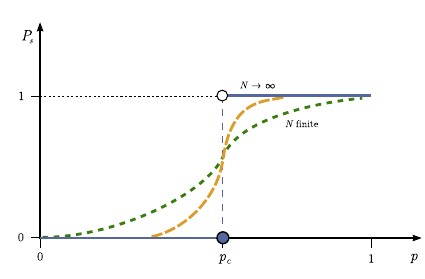
\includegraphics[width=\imsize]{probabilidad}
	\caption[Gráfico esquemático que ilustra la relación entre la probabilidad de percolación y la ocupación en un sistema]{Gráfico esquemático que ilustra la relación entre la probabilidad de percolación y la ocupación en un sistema. A medida que el tamaño del sistema ($N$) se aproxima a infinito, la probabilidad de percolación ($P_\infty$) converge hacia una función escalonada alrededor del umbral crítico ($p_c$). En determinados casos de sistemas altamente específicos, se observa una intersección en un punto único para todos los gráficos correspondientes a valores finitos de $N$. Sin embargo, debido a las correcciones de tamaño finito inherentes, en general esta intersección no ocurre en un único punto para sistemas finitos.}\label{fig:probabilidadinf}
\end{figure}

Es relevante destacar que, en general, los enlaces de una red tienen más vecinos cercanos que los sitios. Por lo tanto, los clústeres de enlaces se forman de manera más eficiente que los clústeres de sitios, lo que implica que se requiere una menor concentración de enlaces para generar un clúster expansivo. En otras palabras, el umbral de percolación de los enlaces es menor que el umbral de percolación de los sitios en una red dada \cite{bunde_fractals_2012}.



Dentro del campo de la percolación, un tema de investigación activo es la determinación precisa de los umbrales de percolación, ya sea mediante métodos exactos o simulaciones. Estos umbrales son una característica fundamental en la teoría de la percolación y su valor no es universal, sino que depende en gran medida de la estructura del grafo subyacente y su dimensionalidad. Se postula que los umbrales alcanzan valores de campo medio solo en el límite de dimensionalidad infinita \cite{Artem,fisher_clúster_2004}. Encontrar pruebas rigurosas de los umbrales y límites exactos ha sido un desafío constante para los investigadores \cite{kesten_critical_1980,wierman_bond_1984,grimmett_percolation_2013}. Aunque se han obtenido los umbrales exactos en 2D para redes cuadradas, triangulares, de panal y estructuras similares utilizando la transformación estrella-triángulo (ver \Cref{table:umbral}) \cite{wierman_bond_1984}, aún existen numerosos sistemas de interés para los cuales los umbrales exactos son desconocidos

 
 \begin{table}[h!]
 	\centering
 	\caption[Umbrales de percolación para varias redes en diferentes dimensiones y la red de Bethe. ]{ Umbrales de percolación para varias redes en diferentes dimensiones y la red de Bethe. La segunda columna enumera el número de vecinos más cercanos (nn), también conocido como número de coordinación. En una dimensión dada, se observa una disminución del umbral de percolación a medida que aumenta el número de vecinos más cercanos. La red o árbol de Bethe es una red no periódica infinita sin bucles cerrados (circuitos), en la cual cada sitio (excepto los múltiples sitios en la superficie) tiene un número de coordinación $Z$, que representa el número de enlaces conectados a dicho sitio.
 	}
 	\begin{tblr}{colspec={X[l,2]X[l,1]X[l,3]X[l,3]},
 			row{odd} = {bg=gray8},
 			row{even} = {bg=gray9},
 			row{1} = {bg=red3, fg=white, font=\sffamily},
 		}
 		
 		red	&  \# nn  &  {Percolación \\ de sitios}  &   {Percolación \\ de enlaces} \\
 		1d & $2$  & $1$ & $1$ \\
 		Triangular (2d) & $6$ &  $1/2$ & $2\sin(\pi/18)\approx 0.34729$ \\
 		Cuadrada (2d) &  $4$ &  $0.592746$ &  $1/2$ \\
 		Panal (2d)        &  $3$ &  $0.6962$ &  $1-2\sin(\pi/18)\approx0.65271$ \\
 		FCC (3d)           &  $12$ &  $0.198$   &  $0.119$ \\
 		BCC (3d)          &  $8$ & $0.246$    &  $0.1803$ \\ 
 		CS (3d) & $6$ &  $0.31161$ &  $0.248814$ \\
 		Diamante (3d) & $4$ & $0.43$ & $0.388$ \\
 		Hipercubo (4d) & $8$ & $0.197$ & $0.1601$ \\
 		Hipercubo (5d) & $10$ & $0.141$ & $0.1182$ \\
 		Hipercubo (6d) & $12$ & $0.107$ & $0.0942$ \\
 		Hipercubo (7d) &  $14$ & $0.089$ &  $0.0787$ \\
 		red de Bethe &  $z$ & $1/(z-1)$  &  $1/(z-1)$  \\
 	\end{tblr}
 	\label{table:umbral}
 \end{table}
 
 
 
 Consideremos un fragmento de la red cuadrada  $\mathbf{Z}^2$ como ejemplo ilustrativo de la definición anterior. En esta red, los puntos de intersección de las líneas se denominan \textquote{sitios}, mientras que los segmentos que los conectan se conocen como \textquote{enlaces}. En una red cuadrada, cada enlace se encuentra conectado a los seis enlaces vecinos más cercanos, mientras que cada sitio solo tiene cuatro sitios vecinos más cercanos. Se asume que cada sitio puede estar en uno de dos estados posibles: \textquote{vacío} o \textquote{abierto} (también se podría utilizar la terminología de \textquote{permitido}, aunque no existe una terminología universalmente aceptada para estos estados, y se podrían emplear términos como \textquote{encendido} o \textquote{apagado}). Además, se considera que la apertura de un sitio ocurre de manera aleatoria e independiente de sus vecinos, con una probabilidad $p$. En esta red, cada par de sitios vecinos más cercanos está conectado por un enlace. Cuando se observa que un poco más de la mitad de los sitios están abiertos (\Cref{fig:percolacion_enlaces_sitios}b, centro), se evidencia una tendencia de los sitios abiertos a agruparse en clústeres de diversas formas y tamaños. Estos clústeres pueden ser clasificados de acuerdo a su tamaño. Por ejemplo, un grupo de tamaño $1$ corresponde a un solo sitio abierto sin vecinos abiertos inmediatos, mientras que un grupo de tamaño $2$ consiste en dos sitios abiertos adyacentes sin vecinos abiertos, y así sucesivamente.
 
 
 
 Cuando la probabilidad $p$ se incrementa a $0.605$ (\Cref{fig:percolacion_enlaces_sitios}b, derecha), se observan varios fenómenos significativos. 
 En primer lugar, con una probabilidad entre $1/2$ y $2/3$, muchos de los sitios se unen en un \textquote{clúster gigante} que abarca tanto la matriz en sentido vertical como horizontal . Esta probabilidad crítica $p_c$, es aproximadamente $p_c \approx 0.593$  para los sitios de la red cuadrada. Un enfoque analógico se puede realizar considerando un \textquote{fluido} que únicamente puede fluir a través de los enlaces que conectan sitios abiertos. Por debajo del umbral de la probabilidad crítica, la red presenta una conductividad cero, mientras que por encima de dicho umbral, la conductividad aumenta a medida que se incrementa la probabilidad. De esta manera, se establece una fuerte relación entre la conectividad de los elementos microscópicos del sistema y las propiedades físicas a nivel macroscópico. Además, a medida que se incrementa la proporción de sitios abiertos, también aumenta la proporción de sitios vacíos con vecinos abiertos. Este aumento en la proporción de sitios vacíos conectados a vecinos abiertos tiene implicaciones significativas en el comportamiento global del sistema.
 
  

\begin{figure}[ht]
	\centering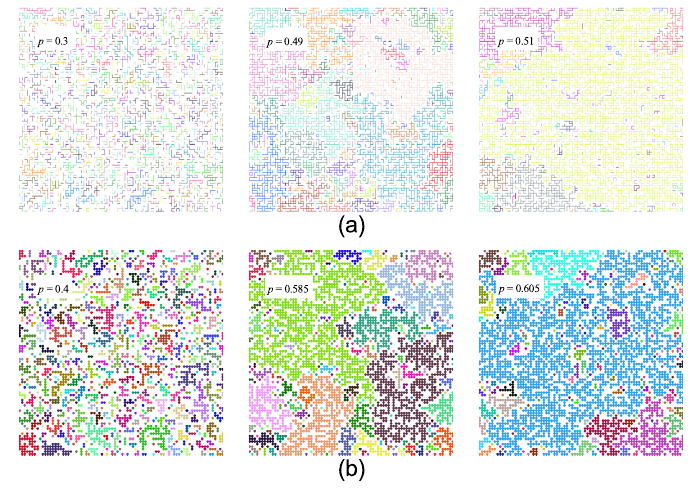
\includegraphics[width=\imsize]{percolacion_enlaces_sitios.png}
	\caption[Diagramas esquemáticos que ilustran la percolación clásica en una red cuadrada.]{Diagramas esquemáticos que ilustran la percolación clásica en una red cuadrada. En estos diagramas, se utilizan diferentes colores para representar clústeres distintos. El tamaño del sistema utilizado es $N = L \times L = 80 \times 80$. Los valores de $p$ etiquetados en las figuras corresponden a las probabilidades de ocupación de los sitios o enlaces correspondientes. (a), se muestra la percolación de enlaces, donde se omiten los sitios y enlaces no ocupados para facilitar la identificación. Para un valor de $p = 0.51$, se observa la existencia de un clúster gigante destacado en color amarillo.(b), se ilustra la percolación de sitios, nuevamente omitiendo los enlaces y sitios no ocupados para una mejor visualización. Para $p = 0.605$, se identifica un clúster gigante en color azul (adaptado de \protect\cite{li_percolation_2021}).}\label{fig:percolacion_enlaces_sitios}
\end{figure}


Una vez que se supera el umbral crítico $p_c$, se observa que el flujo de fluido en la red ocurre exclusivamente a través de los enlaces que conectan los sitios abiertos. Al examinar la estructura resultante, se evidencia la presencia de una columna vertebral compuesta por enlaces que permiten el flujo continuo del fluido, mientras que otros enlaces se convierten en callejones sin salida aislados o ramas colgantes. La proporción de estas ramas varía en función del valor de $p$. La función de accesibilidad se define como la proporción de sitios abiertos que forman parte del clúster infinito, es decir, aquellos que serían atravesados por el fluido en los límites de la red.  A medida que incrementa el valor de $p$, los clústeres experimentan un crecimiento y se fusionan entre sí, mientras que los sitios vacíos se fragmentan y se agrupan en clústeres más pequeños. Cabe destacar que el ejemplo mencionado anteriormente corresponde a la percolación de sitios, donde se varía exclusivamente la proporción de sitios abiertos. Existe también un procedimiento similar conocido como percolación de enlaces, en el cual se varía la proporción de enlaces abiertos (\Cref{fig:percolacion_enlaces_sitios}a). Es importante tener en cuenta que estos dos procedimientos no son intercambiables y no existe una fórmula simple que permita predecir la percolación de enlaces a partir de la percolación de sitios. Además, el valor crítico $p_c$ para la percolación de sitios siempre es mayor que el valor crítico $p_c$ para la percolación de enlaces (consultar \Cref{table:umbral}).


El contorno irregular y \textquote{ramificado} de un clúster en percolación presenta similitudes con los fractales. De hecho, se ha demostrado que los clústeres cercanos al umbral de percolación exhiben propiedades fractales \cite{aharony_introduction_2017}. La dimensión fractal de un clúster de percolación es aproximadamente constante ($D \approx 1.896$) independientemente del tipo de red bidimensional utilizada, ya sea cuadrada, triangular, de panal, de Voronoi u otra (\Cref{fig:distitnasredes}a–d), a pesar de las diferencias en sus conectividades, las cuales pueden ser cuantificadas mediante el número de coordinación $z$, definido como el promedio de enlaces por sitio. No obstante, la dimensión fractal varía según la dimensionalidad o la dimensión de incrustación $d$ de la red. Por ejemplo, los clústeres que se percolan en redes bidimensionales presentan dimensiones fractales distintas a las de las redes tridimensionales, como las redes cúbicas (\Cref{fig:distitnasredes}e).



\begin{figure}[ht]
	\centering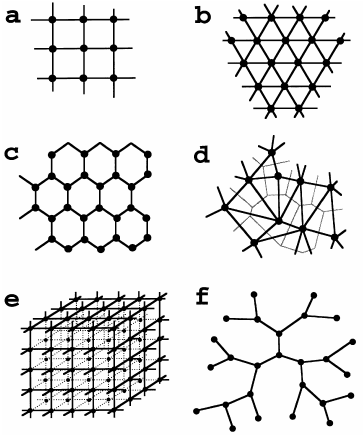
\includegraphics[width=\imsize]{distitnasredes.png}
	\caption[Ejemplos de redes bidimensionales.]{ Ejemplos de redes bidimensionales, en las cuales los sitios son representados por círculos, mientras que los enlaces se muestran mediante líneas oscuras. En esta figura, se exhiben diversas configuraciones de redes: (a) una red cuadrada con  $z=4$, (b) una red triangular con  $z=6$, (c) una red tipo panal con $z=3$, (d) una red Voronoi con un grado promedio de conectividad de $\left\langle z \right\rangle = 6$, (e) una red cúbica con  $z=6$, y (f) un árbol de Cayley con  $z=3$ (adaptado de \protect\cite{berkowitz_percolation_1998})}\label{fig:distitnasredes}
\end{figure}






\section{Fundamentos matemáticos de la percolación}\label{sec:matematicaspercolacion}

Se considera un grafo $\mathcal{G}=(\mathcal{V},\mathcal{E})$, donde $\mathcal{V}$ representa el conjunto de vértices y $\mathcal{E}$ el conjunto de aristas. En el marco del modelo de percolación de enlace, cada arista tiene la capacidad de abrirse de manera independiente con una probabilidad $p$ o cerrarse con una probabilidad $1-p$. Este fenómeno se describe mediante la medida de probabilidad $P_p$. El conjunto de aristas abiertas forma así un subgrafo aleatorio de $\mathcal{G}$ y la pregunta original formulada por Broadbent se centra en determinar si la componente conexa del origen en este subgrafo aleatorio es finita o infinita \cite{beffara_percolation_2006}.



Se define un camino en $\mathcal{G}$ como una secuencia $v_1, v_2, \cdots$ en la cual cada par de vértices sucesivos, $v_i$ y $v_{i +1}$, se encuentran conectados mediante una arista en $\mathcal{G}$. Un camino se considera abierto si todas las aristas $\left\{v_i,v_{i+1}\right\}$ que lo componen están en estado abierto. El clúster infinito del origen se refiere a la existencia de un camino abierto ilimitado que se origina en el vértice de origen. Además, se presenta un modelo análogo denominado percolación del sitio, en el cual todas las aristas son transitables, aunque cada vértice puede encontrarse en estado abierto o cerrado de manera independiente, con probabilidades $p$ y $1 - p$, respectivamente. En este caso, se define un camino abierto como aquel en el cual todos los vértices a lo largo del camino se encuentran en estado abierto.

 Se asume que todos los grafos considerados son conexos, localmente finitos y cuasi-transitivos. Si $A$ y $B$ son subconjuntos de vértices en $\mathcal{V}$, se establece que $A\leftrightarrow B$ si existe un camino abierto que conecta algún vértice en $A$ con algún vértice en $B$. Para simplificar la notación, se utiliza la notación $u \leftrightarrow v$ para denotar la existencia de un camino entre los vértices $u$ y $v$, es decir, el evento $\left\{u\right\} \leftrightarrow \left\{v\right\}$. El clúster abierto $C(v)$  de un vértice $v$ se define como el conjunto de todos los vértices abiertos que se encuentran conectados a $v$ mediante un camino abierto:

\begin{equation}\label{eq:1}
	C(v) = \left\{u\in \mathcal{V}: u \leftrightarrow v \right\}
\end{equation}

La probabilidad de percolación $\theta(p)$  se considera el parámetro central en la teoría de la percolación, y representa la probabilidad de que un sitio seleccionado aleatoriamente pertenezca a un clúster infinito \cite{torquato_percolation_2002}. Es importante resaltar que $\theta(p)$  siempre es menor que $p$, excepto en el caso trivial cuando $\theta(p) = p = 1$. En un sistema infinito, la probabilidad de percolación es cero para valores de $p$ por debajo de $p_c$.


\begin{equation}\label{eq:2}
\theta(p)  \equiv P_\infty = P_p\left\{\mathbf{0} \leftrightarrow \infty\right\} = P_p\left\{\left| C(\mathbf{0})\right|=\infty \right\}  = \begin{cases}
	0 & \text{sí } p<p_c\\
	>0 & \text{sí } p>p_c
\end{cases}
\end{equation}

El modelo de percolación se distingue por su propiedad más destacada: la presencia de una transición de fase geométrica, en la cual el parámetro $\theta(p)$ desempeña el papel de un parámetro de orden en una transición de fase termodinámica. Esta transición se produce en un valor crítico $p_c \in  [0 , 1]$, donde el comportamiento global del sistema experimenta cambios sustanciales en dos regiones distintas: $p < p_c$ y $p > p_c$.  Para definir esta propiedad de forma rigurosa, se emplea la construcción conjunta de sistemas de percolación de Hammersley \cite{broadbent_percolation_1957}  en el grafo $\mathcal{G}$. Se considera una colección de variables aleatorias independientes $\left\{U(v),v\in\mathcal{V}\right\}$, distribuidas uniformemente en el intervalo $[0,1]$. Un vértice $v$ se declara como $p$-abierto si $U(v) \leq p$; de lo contrario, se declara como $p$-cerrado. La configuración de vértices $p$-abiertos sigue la distribución $P_p$ para cada valor de $p\in [0, 1]$. Es relevante destacar que la colección de vértices $p$-abiertos no disminuye a medida que $p$ aumenta, lo que implica que $\theta(p)$ también es una función no decreciente. Esta propiedad se puede demostrar observando que $\theta(0) = 0$ y $\theta(1) = 1$  (ver \Cref{fig:probabilidadtheta}). Por lo tanto, $\theta(p)$  juega un papel fundamental como parámetro de orden en la transición de fase.



\begin{figure}[ht]
	\centering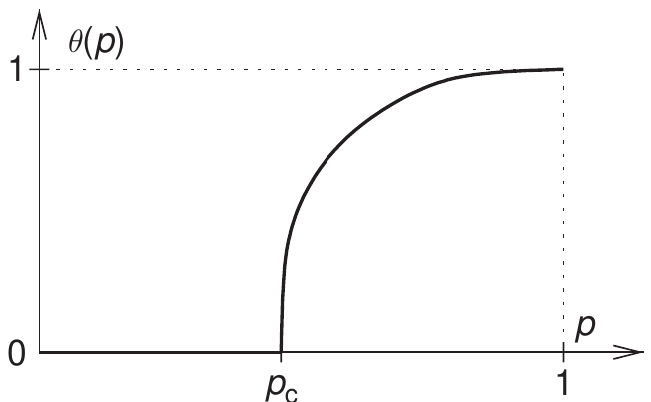
\includegraphics[width=\imsize]{probabilidadtheta.png}
	\caption[El comportamiento de la función $\theta(p)$ en las cercanías del punto crítico.]{El comportamiento de la función $\theta(p)$ en las cercanías del punto crítico.}\label{fig:probabilidadtheta}
\end{figure}


El valor crítico o umbral de percolación $p_c$ se define formalmente (para un sistema infinito) como:

\begin{equation}\label{eq:3}
p_c \equiv p_c( \mathcal{G}) = \sup\left\{p:\theta(p)=0\right\},
\end{equation}


donde $\sup$ representa el supremo, es decir, el límite superior mínimo. Cuando $p < p_c$, el clúster abierto que contiene el origen es finito, lo que implica que todos los clústeres también son finitos. En contraste, cuando $p > p_c$, la distribución $P_p$ presenta una probabilidad estrictamente positiva de que el clúster que contiene el origen sea infinito. Por lo tanto, $p_c$ marca la transición en la cual el comportamiento global del sistema experimenta un cambio significativo.



\begin{theorem}[Ley Cero-Uno de Kolmogórov] % Specify a name/title in square brackets, or leave them out for no title
	Sea $\omega(e)_e$  una secuencia de variables aleatorias independientes e idénticamente distribuidas, y $A$ un evento de cola. Entonces, se cumple que $\mathbb{P}[A] \in {0, 1}$ .
\end{theorem}

La Ley Cero-Uno de Kolmogórov establece que 

\begin{equation}\label{eq:4}
P_p\left\{\left| C(v)\right| =\infty \ \text{para algún} \ v \in  \mathcal{V}  \right\} = 1 \ \text{para} \quad p>p_c
\end{equation}

Esta ley implica que cuando el valor de $p$ supera el umbral $p_c$, se garantiza que al menos un vértice $v \in \mathcal{V}$ pertenezca a un clúster de tamaño infinito.
Por lo tanto, si los intervalos $[0, p_c)$ y $(p_c, 1]$ no están vacíos, se produce una transición de fase en $p_c$. Esta transición de fase indica un cambio cualitativo en el comportamiento del sistema al cruzar el umbral $p_c$.  Utilizando el argumento de Peierls, es posible demostrar de manera sencilla que $p_c(\mathcal{G} )$ es mayor que cero para cualquier grafo $\mathcal{G}$ con un grado acotado. Este resultado implica que en todos los grafos $\mathcal{G}$  con grados acotados, se establece un valor umbral $p_c$ por encima del cual el sistema exhibe una fase supercrítica, donde es probable la existencia de clústeres de tamaño infinito.


\section{La percolación como fenómeno crítico}\label{sec:percolacion_critico}


En la sección anterior, se exploró la percolación como una transición de fase geométrica  que ocurre cuando la concentración crítica $p_c$ divide el sistema en dos fases distintas: una con clústeres finitos ($p < p_c$) y otra con un clúster de gran tamaño ($p > p_c$). Es importante destacar que una verdadera transición de fase se presenta únicamente en sistemas infinitos, conocidos como el \textquote{límite termodinámico}. En este contexto, la concentración crítica $p_c$ se define de forma única en sistemas infinitos. La transición de percolación se caracteriza por las propiedades geométricas de los clústeres cercanos a $p_c$. Un parámetro clave en este sentido es la probabilidad $P_\infty$, definida mediante la  \cref{eq:2}. Esta probabilidad es nula por debajo de $p_c$ y distinta de cero por encima de $p_c$. Para valores ligeramente superiores a $p_c$, se establece una relación de la forma

 \begin{equation}\label{eq:10}
	P_\infty \propto \left(p-p_c\right)^\beta,
\end{equation}

donde $\beta$ es el \textquote{exponente crítico}. El comportamiento crítico en la teoría de la percolación se refiere al estudio de la red infinita y los clústeres grandes pero finitos en las cercanías de $p_c$, también conocido como región de escalamiento. En esta región, se observa un comportamiento crítico independiente de las propiedades locales del sistema, como el tipo de red y el mecanismo de percolación. Esto se debe al principio de universalidad, que establece que el valor de $p_c$ está determinado por la estructura local del sistema, mientras que el comportamiento de los clústeres cercanos a $p_c$ es independiente de dicha estructura local. En consecuencia, la percolación se considera un fenómeno dependiente del sustrato pero independiente del modelo específico. Los exponentes críticos, como $\beta$, son determinados exclusivamente por la geometría del sistema y son idénticos tanto en la percolación de enlaces como en la percolación de sitios.

 \subsection{Parámetro de orden}\label{sec:parametro_orden}
 
 
 
 
 
La teoría de escalamiento de los clústeres de percolación es el enfoque más elegante para caracterizar la percolación como un fenómeno crítico \cite{stauffer_scaling_1979}. En términos de estadísticas de clústeres, se puede formular gran parte de la teoría de la percolación, lo que facilita establecer analogías con otras transiciones de fase. En este sentido, se propone la definición de un parámetro de orden que permita caracterizar nuestro modelo de criticidad neuronal a través de observables geométricos. En el contexto de la percolación, los clústeres desempeñan un papel fundamental.
 
 
\begin{definition}[clúster] % Specify a name/title in square brackets, or leave them out for no title
Un clúster se define como  un conjunto de componentes o elementos interconectados en una red, donde la conexión entre ellos se establece mediante vínculos o relaciones específicas.
\end{definition}

Se consideran clústeres de tamaño unitario a los nodos aislados, mientras que se denomina $s$-clúster a cualquier conjunto de $s$ nodos conectados. El análisis de la percolación se centra en la aparición del clúster infinito a medida que aumenta la probabilidad $p$. Una medida común para caracterizar este fenómeno es la probabilidad $\bar{S}_1/N$ de que un nodo pertenezca al clúster infinito, donde $N$ representa el tamaño del sistema (número de sitios) y $\bar{S}_1$ es el promedio en ensamble del número de sitios $S_1$ en el clúster más grande.  Como se ilustra en la \cref{fig:probabilidadtheta}, a medida que $p$ aumenta, también lo hace la probabilidad de encontrar clústeres de mayor tamaño. En una red finita, como se muestra en la \cref{fig:percolacion_enlaces_sitios}, se identifica un valor crítico $p_c$ por encima del cual al menos un clúster conecta los extremos \textquote{inferior} y \textquote{superior} (o \textquote{izquierdo} y \textquote{derecho}) de la red. En otras palabras, se establece un punto crítico $p_c$ para el cual $\bar{S}_1/N$ adquiere un valor distinto de cero. En el campo de la ciencia de redes, el tamaño del clúster más grande se considera un parámetro de orden preferido. En el umbral de percolación, este parámetro de orden muestra un comportamiento crítico a medida que el sistema tiende al límite $N \to\infty$. Dicha relación puede expresarse de la siguiente manera:

\begin{equation}\label{eq:5}
	P_\infty = \lim_{N\to\infty} \frac{\bar{S}_1}{N} =  \begin{cases}
		0 & \text{sí } p<p_c\\
		a\left(p-p_c\right)^\beta & \text{sí } p>p_c
	\end{cases}
\end{equation}

donde $a$ representa una constante y $\beta$ es el exponente crítico del parámetro de orden. La formulación basada en la teoría de escalamiento de los clústeres de percolación permite una caracterización precisa de la transición de fase en el modelo de criticidad neuronal abordado en esta parte de la tesis. Al introducir un parámetro de orden, se establece una conexión rigurosa entre las propiedades estadísticas de los clústeres y la dinámica coordinada de la actividad neuronal en el organismo modelo C. elegans. 


\subsection{ El tamaño promedio de los clústeres  $ \chi(p)$}\label{sec:Sucebtibilidad}

Como la percolación es un proceso estocástico se da lugar a la formación de clústeres con una amplia variedad de tamaños y formas en diversas redes \cite{aharony_introduction_2017}. Para analizar las propiedades estadísticas promedio de estos clústeres, es necesario examinar sus distribuciones. En particular, se investiga la distribución del tamaño de los clúster  \( p_s=\frac{m_s}{\sum_{s}m_s} \), donde $m_s$ representa el número de clústeres de tamaño $s$ presentes en una red de tamaño $N$. Además, se utiliza comúnmente la distribución normalizada de tamaño de clústeres, \(n_s=\frac{m_s}{N}\), que indica la cantidad de clústeres de tamaño $s$ por nodo en la red, considerando la probabilidad de percolación $p$ \cite{barrat_dynamical_2008}. La probabilidad de que un nodo $i$ pertenezca a un clúster de tamaño $s$ se denota como $sn_s(p)$, donde $i$ puede ser cualquier elemento del clúster en cuestión. Es importante destacar que \(p_s=\frac{n_sN}{\sum_{s}m_s}=n_s\left\langle S \right\rangle \), donde \(\left\langle S \right\rangle =\frac{N}{\sum_{s}m_s} = \sum_{s} sP_s \) representa el tamaño promedio del clúster. Cabe señalar que el tamaño promedio \(\left\langle  S \right\rangle \)   difiere del tamaño promedio de clúster \(\chi\) , el cual se define más adelante. La probabilidad $p$ de que un sitio esté ocupado se puede expresar como la suma de estas probabilidades para todos los tamaños posibles. En el caso de $p < p_c$, esta relación se formula de la siguiente manera:

\begin{equation}\label{eq:12}
p=\sum_{s}{sn_s}(p)
\end{equation}

Cuando $p > p_c$, se observa la presencia de un clúster gigante, en el cual cada nodo tiene una probabilidad finita $\bar{S}_1/N > 0$ de formar parte del mismo. Por otro lado, los demás clústeres presentan un tamaño finito $s$ para cualquier valor arbitrario de $p$, y su comportamiento se describe mediante la distribución de tamaño de clúster $n_s(p)$. Por lo tanto, la suma de todas las probabilidades de que un nodo dado pertenezca a un clúster de tamaño finito, excluyendo el clúster gigante, debe ser igual a $p$:

\begin{equation}\label{eq:13}
	p=P_\infty+{\sum_{s}}^{\prime}sn_s(p) 
\end{equation}

Aquí, la suma ${\sum_{s}}^{\prime}$ abarca todos los valores finitos de $s$, lo cual implica que el clúster gigante se excluye de dicha suma. Resulta primordial establecer una medida objetiva para cuantificar con precisión el tamaño de los clústeres.  Al analizar el fenómeno de la percolación, se observa de manera intuitiva que, a medida que el valor de $p$ disminuye, el tamaño de los clústeres es pequeño, mientras que su tamaño tiende a aumentar a medida que $p$ se incrementa, hasta llegar a un umbral crítico donde el clúster gigante adquiere un rol dominante, por lo que el tamaño de los clústeres debe divergir \cite{saberi_recent_2015}. No obstante, una vez superado dicho umbral, es imperativo excluir al clúster gigante de los análisis, ya que su presencia constante puede sesgar los resultados. Además, a medida que los clústeres son absorbidos por el clúster gigante, el tamaño promedio de los clústeres restantes vuelve a disminuir. Por consiguiente, buscamos una medida que exhiba un comportamiento creciente, divergente en el umbral crítico y, posteriormente, decreciente (véase la \Cref{fig:promedio}). Aplicando el teorema de Bayes, podemos expresar de forma rigurosa la probabilidad condicional de que un nodo ocupado pertenezca a un clúster de tamaño $s$ mediante la siguiente formulación:

\begin{equation}\label{eq:14}
w_s(p) = \frac{sn_s(p)}{{\sum_{s}}^{\prime}sn_s(p)}
\end{equation}

Con base en esto, definimos el tamaño promedio de los clústeres $\chi(p)$  a los cuales pertenece cualquier nodo ocupado como:

\begin{equation}\label{eq:15}
\chi(p)={\sum_{s}}^{\prime}{sw_s(p)}=\frac{{\sum_{s}}^{\prime}{s^2n_s(p)}}{{\sum_{s}}^{\prime}{sn_s(p)}}
\end{equation}

Es importante resaltar que, al considerar las sumas ${\sum_{s}}^{\prime}$, no se toma en cuenta la divergencia generada por la presencia del clúster gigante. Sin embargo, la definición proporcionada por la \cref{eq:15} carece de información sobre la estructura de los clústeres, como su compacidad y extensión espacial. No obstante, resulta imprescindible abordar esta limitación y analizar la extensión geométrica de los clústeres. Para tal propósito, se consideran los sitios pertenecientes a un clúster de tamaño $s$, representados por las coordenadas $\mathbf{r}_i$, donde $i = 1, 2,\cdots,s$. Con el fin de examinar de manera más exhaustiva la estructura interna, se introduce el concepto de centro de masa del clúster, $\mathbf{r}_0 = \sum{\mathbf{r}_i}/s$, definido como el promedio de las coordenadas de los sitios, dividido por el tamaño del clúster $s$. A partir de esta definición, se plantea el concepto de radio de giro del clúster, $R_s$, que se obtiene al calcular la raíz cuadrada de la suma de las distancias al cuadrado entre cada sitio y el centro de masa, dividida por el tamaño del clúster $s$:

\begin{equation}\label{eq:19}
R_s^2=	\frac{\sum{\left(\left| \mathbf{r}_i-\mathbf{r}_0\right|^2 \right)}}{s}=\frac{1}{2s^2}\sum_{i,j}{\left|\mathbf{r}_i-\mathbf{r}_j\right|^2}
\end{equation}

Este parámetro permite evaluar la distancia promedio entre dos sitios dentro del mismo clúster. Un valor menor de $R_s$ indica una mayor compacidad y una menor extensión espacial del clúster en cuestión. Adicionalmente, otro aspecto relevante para describir la estructura de los clústeres es la longitud de correlación, $\xi$. Esta medida se basa en la función de correlación de dos puntos, $g_c(r )$, que representa la probabilidad de que dos puntos se encuentren en el mismo clúster, dada una distancia $r$ entre ellos. Por lo general, esta función sigue un patrón de decaimiento exponencial expresado como:


\begin{equation}\label{eq:16}
g_c(r) \sim e^{-r/\xi},  \ r\to\infty
\end{equation}

La longitud de correlación, $\xi$, constituye una escala característica de la distribución de clústeres y establece la distancia máxima a partir de la cual los clústeres se vuelven escasos de manera exponencial. Además, $\xi$ delimita la región de escala en la cual los clústeres de percolación exhiben un comportamiento autosimilar. Para calcular $\xi$, se utiliza la siguiente relación:

\begin{equation}\label{eq:17}
\xi^2=\frac{\sum_r{r^2g_c(r)}}{\sum_r{g_c(r)}}
\end{equation}

Dentro de esta expresión, se reemplaza $r^2$  en la suma anterior por el cuadrado de la distancia promedio entre dos puntos del clúster, es decir, $2R_{s}^2$. Asimismo, considerando la probabilidad $sn_s$ de que un punto pertenezca a un clúster de tamaño $s$ y teniendo en cuenta que dicho punto está conectado a $s$ sitios, se sustituye $g_c(r)$ por $s^2n_s$. Esto nos lleva a la siguiente relación para el cuadrado de la longitud de correlación:

\begin{equation}\label{eq:18}
	\xi^2(p)=\frac{{\sum_s}^{\prime}{2R_{s}^2s^2n_s(p)}}{{\sum_{s}}^{\prime}{s^2n_s(p)}}
\end{equation}

Estas definiciones de los diferentes parámetros característicos son aplicables en todas las dimensiones $d$.



\begin{figure}[ht]
	\centering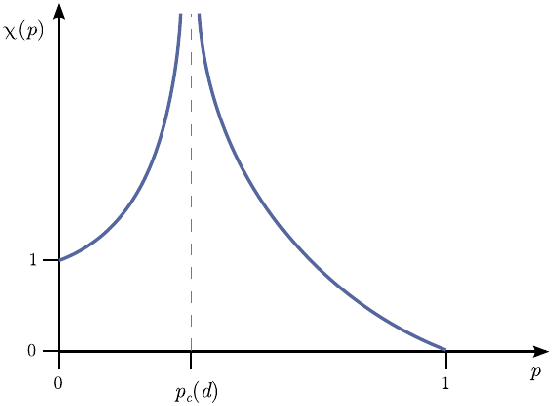
\includegraphics[width=\imsize]{promedio.png}
	\caption[Evolución del tamaño promedio de los clústeres finitos y la longitud de correlación cerca de la transición percolativa.]{ Evolución del tamaño promedio de los clústeres finitos y la longitud de correlación cerca de la transición percolativa. Como se puede observar en el diagrama, al alcanzar el umbral crítico $p_c$, se evidencia la aparición del componente gigante, lo que implica la presencia de clústeres de distintos tamaños en el sistema en estudio. Asimismo, se aprecia que la longitud de correlación experimenta un aumento significativo, indicando una relación proporcional con el tamaño del sistema $L$.}\label{fig:promedio}
\end{figure}


\subsection{Teoría de escala y exponentes críticos}



El comportamiento del proceso de percolación en un sistema está estrechamente ligado a su posición en el régimen subcrítico ($p < p_c$) o supercrítico ($p > p_c$). En el régimen subcrítico, la probabilidad de encontrar un clúster finito $s$ de gran tamaño en un punto dado disminuye exponencialmente con $s$, lo que implica una distribución de tamaños de clúster con una cola de decaimiento exponencial. Esta disminución exponencial puede ser descrita mediante el parámetro $\kappa(p) > 0$, que $\kappa(p) \to\infty$ cuando $p\to0$, y $\kappa(p = p_c ) = 0$. En otras palabras, se puede aproximar la distribución de tamaños de clústeres utilizando la expresión:

\begin{equation}\label{eq:20}
w_s(p) \approx e^{-\kappa(p)s}, \ s\to\infty
\end{equation}

Por otro lado, en el régimen supercrítico, la cola de la distribución de tamaños de clústeres finitos muestra un decaimiento más suave. En este caso, existen dos funciones,  $\kappa_1(p)$  y $\kappa_2 (p)$, que cumplen con $0 < \kappa_2(p) \leq  \kappa_1(p) < \infty$ \cite{grimmett_percolation_2013}, tales que:

\begin{equation}\label{eq:21}
	\exp{\left(-\kappa_1(p)s^{\frac{d-1}{d}}\right)} \leq w_s(p) \leq \exp{\left(-\kappa_2(p)s^{\frac{d-1}{d}}\right)}
\end{equation}

Además, la potencia $s^{(d-1)/d}$, que representa el orden del área superficial de una esfera en $d$ dimensiones con volumen $s$, indica que los clústeres son compactos en la región supercrítica \cite{djordjevic_scaling_1987}. Es importante destacar que, aunque el valor numérico de las cantidades que caracterizan la percolación depende de los detalles microscópicos del sistema, como el número de conexiones entre los nodos, cerca del umbral de percolación $p_c$, la mayoría de estas cantidades siguen leyes de escala que son ampliamente independientes de la estructura de la red y sus detalles microscópicos. En consonancia con la hipótesis de escala, se establece una relación general entre el número $n_s(p)$ de clústeres finitos por sitio y el tamaño $s$, dada por:
\begin{equation}\label{eq:22}
	n_s(p)  \propto s^{-\tau}F\left(c(p)s\right), \ s\to\infty,
\end{equation}

Donde $\tau$ es un exponente libre y $F$ es una función de escala.  Además, cerca del umbral de percolación, se ha observado que  $c(p)$ puede ser descripta mediante una ley de potencia general, $c (p) \propto \left|p-p_c \right|^{1/\sigma}$, donde $\sigma$ es otro exponente crítico.  En relación con la distribución del tamaño de los clústeres, se pueden considerar los $m$-ésimos momentos, definidos como $M_m(p) = \sum_{s}s^mn_s(p)$, con $m \geq 1$. También se ha conjeturado la existencia de relaciones de escala cerca del umbral de percolación que involucran diferentes exponentes críticos, tales como $\beta$, $\gamma$, $\alpha$, $\Delta$,  $\tau$ y $\nu$:


\begin{align} 
	P_\infty(p) & \simeq B\left(p-p_c\right)^\beta, \label{eq:6a}\\ 
	\chi(p)  & \simeq \Gamma^{\pm}\left| p-p_c \right|^{-\gamma}, \label{eq:6b} \\
	n_s(p) & \simeq A^{\pm}  \left| p-p_c \right|^{2-\alpha}, \label{eq:6c} \\
	\frac{M_{m+1}(p)}{M_m(p)} &\simeq D^{\pm} \left| p-p_c \right|^{-\Delta}, \label{eq:6d}\\
	\xi(p) &\simeq f^{\pm}\left| p-p_c \right|^{-\nu}, \label{eq:6e} \\
	s_\xi(p) &\simeq \left| p-p_c \right|^{-\frac{1}{\sigma}}, \label{eq:6f}\\
	p_s &\propto s^{-\tau}.
	\end{align}
	
	
que también definen las amplitudes críticas, donde estas desempeñan un papel crucial al determinar las magnitudes que se acercan al punto crítico ($p_c$), ya sea desde arriba o desde abajo, indicadas por los superíndices $+$ o $-$. Estas amplitudes combinadas proporcionan una forma canónica de codificar la información universal relacionada con la aproximación a la criticidad \cite{aharony_universal_1980}. La caracterización del comportamiento crítico de la transición de percolación se basa en los exponentes  $\beta$, $\gamma$, $\alpha$, $\Delta$,  $\tau$ y $\nu$. Estos exponentes, conocidos como exponentes críticos, describen las propiedades geométricas de la transición y son independientes de los detalles estructurales de la red, como su forma (cuadrada o triangular), así como del tipo de percolación (sitio, enlace o continua). En cambio, su valor depende únicamente de la dimensión $d$ de la red.  La propiedad de universalidad, inherente a las transiciones de fase en general, también se manifiesta en la transición de percolación. En esta transición, el parámetro de orden experimenta una desaparición continua en el punto crítico. Esto se refleja en el comportamiento característico de ley de potencia y funciones singulares observado en el umbral de percolación. Estos fenómenos indican que el sistema exhibe grandes fluctuaciones en sus propiedades estadísticas antes de la aparición de una fase macroscópicamente ordenada, como la formación de una estructura global conexa. Cuando las fluctuaciones alcanzan el tamaño del sistema en el punto crítico, el sistema experimenta una transición hacia una nueva fase con orden macroscópico \cite{barrat_dynamical_2008}.

	
Es importante destacar que todas las cantidades mencionadas se definen en el límite termodinámico de sistemas de gran tamaño \cite{bunde_fractals_2012}. Sin embargo, hasta el momento, no se ha logrado obtener cálculos exactos y rigurosos de los exponentes críticos para la percolación, ni siquiera para otras transiciones de fase \cite{stauffer_scaling_1979}. El objetivo de una teoría de escala, en este contexto, es establecer relaciones entre estos exponentes críticos. Dicha teoría se basa en un enfoque fenomenológico que se limita a relacionar magnitudes medibles sin requerir el cálculo directo de las mismas. Asimismo, es importante tener presente que los exponentes no son independientes entre sí, sino que satisfacen las relaciones de escala expresadas por:


 \begin{align}\label{eq:7}
 	&\beta = \Delta\left(\tau-2\right)=\frac{\tau-2}{\sigma},\\
 	&\gamma=\frac{3-\tau}{\sigma},\\
 	&2-\alpha= \gamma + 2\beta =\frac{\tau-1}{\sigma}.\\	
 	 \end{align}



\subsection{ Teoría de  escala en el número de clústeres }


Se pretende determinar el comportamiento asintótico del número de clústeres en el umbral, $n_s(p_c)$.  Se ha observado una relación proporcional entre el tamaño de los clústeres y su segundo momento, expresada como  $\chi \propto \sum_s s^2n_s$,   la cual se mantiene constante en el umbral debido a un denominador finito.  
Sin embargo, cuando $p = p_c$, esta suma se vuelve infinita, mientras que para cualquier otro valor de $p$ permanece finita. Se postula que un decaimiento de ley de potencia es más plausible para el número de clústeres $n_s(p_c)$, lo cual implica que el tamaño promedio de los clústeres, $\chi$, seguiría siendo finito en $p = p_c$. Por lo tanto, se define el exponente $\tau$ de Fisher (modelo de gotas de Fisher \cite{fisher_theory_1967}) mediante la relación $n_s(p_c) \propto s^{-\tau}$, considerando valores grandes de $s$. Con el fin de minimizar los errores en los cálculos numéricos, es común calcular la función de distribución acumulada complementaria (CCDF) de la distribución de tamaños de clústeres, que representa la probabilidad de que los clústeres tengan un tamaño mayor que $s$,

\begin{equation}\label{eq:36}
CCDF=P_{acc}(s)=\int_{0}^{\infty}n_sd_s=\int_{0}^{\infty}{s^{-\tau}}ds\propto s^{1-\tau}
\end{equation}
En este contexto, la distribución de clústeres sigue una relación de escala:


\begin{equation}\label{eq:37}
n_s\sim s^{1-\tau}f\left(\frac{s}{s^{*}}\right) \ \text{donde} \ s^*=\left| p_c-p\right|^{-\frac{1}{\sigma}}
\end{equation}

Es importante destacar que, en el caso de redes con tamaño finito $N < \infty$, la distribución de clústeres sigue una relación de escala modificada expresada como:

\begin{equation}\label{eq:38}
P(s)\sim s^{1-\tau}g\left(\frac{s}{s^\prime}\right) \ \text{donde} \ s^{\prime} \sim \xi^{d^c_f}
\end{equation}

Además, al asumir que $\xi\sim L$, podemos inferir que

\begin{equation}\label{eq:39}
s^{\prime} \sim L^{d_f^c}\sim N^{\frac{d_f^c}{d}}
\end{equation}

En las redes con tamaño $N < \infty$, el valor de $s^{\prime}$ es proporcional al tamaño del segundo clúster más grande ($S_2$) en la red ($S_2 \propto  s^{\prime}$). Por lo tanto, para derivar la dimensión fractal, se utiliza el valor de $S_2$, lo cual resulta útil para analizar la estructura de los clústeres en la red y obtener información relevante \cite{tesis_Mahdi}.



\subsection{Estructura fractal de los clústeres en el fenómeno de percolación}

La teoría de la escala postula que el comportamiento de un sistema, cuando se analiza a escalas de longitud inferiores a la longitud de correlación $\xi$, se asemeja al estado umbral. En el punto crítico, donde $\xi$ representa la única escala de longitud que determina el comportamiento crítico de una red infinita, la longitud de correlación tiende a infinito ($\xi\to\infty$). Esta desaparición de escala en $p = p_c$ evoca la invariancia de escala, la cual implica la aparición de autosimilitud en las características geométricas de los clústeres de percolación. En el contexto de los clústeres de percolación, las propiedades fractales persisten incluso cuando $p = p_c$ y $\xi$ es finita, siempre y cuando la escala de longitud utilizada para el estudio del sistema sea menor que $\xi$. Sin embargo, una vez que se supera la longitud de correlación, la geometría adquiere una forma euclidiana. Para una comprensión más precisa de este fenómeno, se considera un sistema de percolación observado a través de una ventana hipercúbica de tamaño $L^d$, donde $L$ representa el tamaño lineal de la ventana o puede interpretarse como el tamaño de un sistema finito.

Dentro del marco teórico de la invariancia de escala, se deduce que la masa media $M$ de los clústeres dentro de la ventana aumenta siguiendo una ley de potencias en relación con el tamaño, es decir, $M(\xi,L)\sim L^{d_f^c}$, donde $d_f^c$ representa la dimensión fractal del clúster. Esta dimensión fractal describe cómo, en promedio, la masa $M$ del clúster dentro de una esfera de radio $r $ escala con $r$:

\begin{equation}
	M(r)\sim r^{d_f^c}.
\end{equation}

En el caso de los fractales aleatorios, $M(r)$ representa el promedio de múltiples configuraciones de clústeres diferentes o, en otras palabras, de muchos centros de esferas distintos en el mismo clúster infinito. Cuando nos encontramos por encima de $p_c$ y trabajamos con escalas de longitud $L\gg\xi$, se considera que el clúster infinito consiste en un objeto homogéneo compuesto por numerosas celdas de tamaño $\xi$. En esta situación, la masa media $M(\xi,L)$ se relaciona con $L^{d_f^c}$ mediante una función de cruce $\mathfrak{m}$:

\begin{equation}\label{eq:23}
M(\xi,L) \sim L^{d_f^c} \mathfrak{m}(L/\xi), \ \text{donde} \  \mathfrak{m}(L/\xi)= \begin{cases}
	\text{constante }& \text{sí } L\ll\xi\\
	\left(\frac{L}{\xi}\right)^{d-d_f^c} & \text{sí } L\gg\xi
\end{cases}
\end{equation}

Además, la masa $M$ es proporcional a $L^dP_\infty$.   Al igualar esta relación con la ecuación \Cref{eq:23} y reescribiendo en términos de $(p - p_c)$ utilizando  la \Cref{eq:6a} y \Cref{eq:6e}, se obtiene la relación de escala:

\begin{equation}\label{eq:24}
d_f^c=d-\frac{\beta}{\nu}
\end{equation}

 La cual proporciona información sobre la dimensión fractal en función de la dimensión del sistema y el exponente crítico $\nu$.  La dimensión fractal $d_f^c$ se determina mediante los exponentes universales $\beta$ y $\nu$, los cuales son independientes de la estructura topológica del sistema. Como resultado, $d_f^c$ se considera una propiedad intrínseca del sistema, invariable ante la configuración espacial.  Cabe destacar que en dimensiones específicas, como $2D$ y $d \geq d_c = 6$, se conocen los valores exactos de $d_f^c$, siendo $d_f^c = 91/48$ y $4$, respectivamente. Sin embargo, en dimensiones distintas, solo es posible obtener estimaciones de $d_f^c$ a través de simulaciones numéricas. Además de las relaciones mencionadas, existen otras interconexiones significativas entre los exponentes críticos y la dimensión fractal, las cuales contribuyen a una mejor comprensión de las transiciones de fase. 

\begin{align}\label{eq:25}
	\frac{1}{d_f^c} &= \sigma\nu,\\
	d\nu &= \gamma + 2\beta	=2-\alpha=\frac{\tau-1}{\alpha}.
\end{align}

En el marco de la teoría de transición de fase, se postula la existencia de una dimensión crítica superior, $d_c$, que en el caso de la percolación es igual a $6$.  Por encima de esta dimensión crítica, los exponentes críticos adquieren los mismos valores que en la teoría de campo medio. En consecuencia, la relación de hiperescala mencionada anteriormente solo se cumple para dimensiones $d \leq d_c$. Esto revela la conexión entre el comportamiento a gran escala del sistema y su estructura topológica en diferentes dimensiones.  Es importante destacar que la estructura geométrica de los clústeres de percolación en dimensiones altas no puede ser completamente explicada mediante analogías con redes aleatorias, a pesar de compartir una naturaleza de campo medio. Esta discrepancia sugiere la existencia de otros factores y mecanismos que influyen en la formación de los clústeres. 

Además, es necesario considerar que el comportamiento crítico por debajo de la dimensión crítica superior $d_c$ difiere de la aproximación de campo medio, que solo es válida fuera de la transición de fase. Para comprender mejor estos sistemas, se recurre a la teoría de grupos de renormalización, la cual ha realizado predicciones significativas sobre el comportamiento de la percolación cerca y en el umbral. Esta teoría proporciona un marco teórico sólido para comprender los fenómenos críticos y la influencia de las fluctuaciones en el sistema. Es relevante mencionar que la teoría del grupo de renormalización también establece la existencia de una dimensión crítica inferior, $d_l$, que en el caso de la percolación se encuentra en $2$ dimensiones. Por debajo de esta dimensión crítica inferior, no se produce una transición de fase, lo cual impone una limitación fundamental en la percolación en dimensiones más bajas.




\subsection{ Escaleo con el tamaño finito (Finite-Size	Scaling,FSS)}\label{sec:escaleo}



Hasta el momento, se ha enfocado el estudio en sistemas de tamaño infinito. Sin embargo, es de suma importancia comprender el comportamiento de las magnitudes que caracterizan la percolación cerca del umbral en sistemas finitos pero de gran escala. En la práctica, es común trabajar con este tipo de sistemas, ya sea a través de la recolección de datos experimentales o mediante simulaciones por computadora. En este contexto, el análisis del escalado con tamaño finito se convierte en una herramienta precisa para determinar los exponentes críticos. Este enfoque, inicialmente introducido por Fisher en el estudio de sistemas térmicos cercanos a su punto crítico \cite{Fisher_critical}, puede ser adaptado para investigar el comportamiento de la percolación. Es esperable que las magnitudes relevantes dependan del tamaño del sistema, y la longitud de correlación $\xi$, definida para sistemas infinitos, desempeña un papel fundamental en este aspecto. Por consiguiente, se espera que existan diferencias significativas en el comportamiento de estas magnitudes cuando consideramos casos donde $L/\xi\gg1$ y $L/\xi \ll 1$ \cite{bunde_fractals_2012}.


En relación a $P_\infty$, se observa que cuando el tamaño del sistema $L$ es mucho mayor que la longitud de correlación $\xi$, el sistema exhibe un comportamiento análogo al de un sistema infinito. En otras palabras, la magnitud $P_\infty$ se vuelve independiente de $L$ y puede ser descripta mediante la relación $P_\infty \propto (p - p_c)^{x}$. Por otro lado, cuando $\xi\gg L\gg1$, el número de sitios del clúster gigante en una \textquote{ventana} se vuelve proporcional a $L^{d_f^c}$. A partir de esta observación, podemos obtener $P_\infty$ dividiendo dicho resultado por el número total de sitios ocupados en la ventana, que corresponde a $pL^d$. Por lo tanto, se concluye que $P_\infty\sim L^{d_f^c-d}$. Dado que la longitud de correlación $\xi$ es la única característica relevante, $P_\infty$ depende exclusivamente de $L$ a través de la relación $L/\xi$, lo cual motiva la formulación del \gls{ansatz} de escala:

\begin{equation}\label{eq:30}
P_\infty\sim \left(p-p_c\right)^AG\left(\frac{L}{\xi}\right)\sim \xi^{-\frac{A}{\nu}}G\left(\frac{L}{\xi}\right)
\end{equation}

Para describir la transición desde el régimen donde $L/\xi\ll1$ hasta el régimen donde $L\xi\gg 1$, es necesario introducir la función de escala $G(x)$. Para obtener los resultados esperados en ambos regímenes, se requiere que se cumpla $A = \beta$  y que:

\begin{equation}\label{eq:31}
G(x) \sim \begin{cases}
	x^{d_f^c-d} & \text{sí } x\ll 1\\
\text{constante} & \text{sí } x\gg1
\end{cases}
\end{equation}


Con el fin de examinar las implicaciones de estas relaciones, imaginemos que llevamos a cabo simulaciones por ordenador de $P_\infty$  en una red triangular. En esta red, la concentración crítica para la percolación de sitios en una red infinita es precisamente de $1/2$. Para dichas simulaciones, se seleccionará una red de considerable tamaño, como $L = 1000$, y se asignarán aleatoriamente los sitios con una probabilidad $p$. Posteriormente, se analizarán los clústeres y se determinará la presencia de un clúster gigante. Este procedimiento se repetirá para $5000$ configuraciones de la red, calculando el promedio de $P_\infty$ en todas ellas.  Cuando la probabilidad $p$ se encuentra sustancialmente por encima del umbral de percolación, donde la longitud de correlación $\xi$ es considerablemente menor que $L = 1000$, no se aprecia el impacto del tamaño finito de la red.  En otras palabras, el comportamiento percolativo se asemeja al de una red infinita. A medida que nos acercamos al valor crítico $p_c$, la probabilidad de encontrar un clúster gigante, $P_\infty$, disminuye siguiendo una ley de potencias, específicamente $\left(p-p_c\right)^\beta$, siempre y cuando el tamaño de la red, $L$, sea significativamente mayor que la longitud de correlación, $\xi$ ($L\gg\xi$). Además, al acercarnos aún más a $p_c$, alcanzamos una concentración de cruce $p^*$, donde el tamaño de la red y la longitud de correlación son comparables ($L \sim \xi$). En el rango entre $p^*$ y $p_c$ donde el tamaño de la red es menor que la longitud de correlación ($L < \xi$), $P_\infty$ se mantiene aproximadamente constante en un valor finito. 

Este fenómeno puede entenderse considerando un sistema finito de $10^6$ sitios, donde un cambio marginal en la concentración equivale, en promedio, a agregar o eliminar tan solo unos pocos sitios ocupados, lo cual tiene un impacto prácticamente insignificante en el sistema. Por tanto, en la red en cuestión, no se aprecia diferencia alguna en $P_\infty$ al comparar $p = p_c + 10^{-6}$ y $p = p_c + 10^{-12}$. No obstante, a medida que incrementamos el tamaño de la red, este ligero cambio en la concentración adquiere mayor relevancia. Además, para el caso de una red infinita, se presentan cambios drásticos en las proximidades de $p_c$. En el ejemplo previamente mencionado, $P\infty$ disminuye en un factor de $10^{6\beta}$, lo cual corresponde a un orden de magnitud de $10$. En consecuencia, resulta conveniente expresar la relación de escala establecida por la \cref{eq:30} en una forma ligeramente alterada. Mediante la multiplicación y división por $L^{-\beta/\nu}$, obtenemos:

\begin{equation}\label{eq:32}
	P_\infty\sim L^{-\frac{\beta}{\nu}}H\left(\frac{L}{\xi}\right) \sim \begin{cases}
		L^{-\frac{\beta}{\nu}} & \text{sí } L\ll \xi\\
		\xi^{-\frac{\beta}{\nu}}& \text{sí } L\gg\xi
	\end{cases},
\end{equation}

donde $H(x)=G(x)x^{\frac{\beta}{\nu}}$.  Así, se evidencia que los efectos del tamaño finito descritos para $P_\infty$ también se manifiestan en la distribución $n_s(p)$ y en otras cantidades relacionadas, como el tamaño promedio de los clústeres:


\begin{equation}\label{eq:33}
	\chi(L,\xi) \sim \begin{cases}
		L^{\frac{\gamma}{\nu}} & \text{sí } L\ll \xi\\
		\xi^{\frac{\gamma}{\nu}}& \text{sí } L\gg\xi
	\end{cases},
\end{equation}
	
En general, si consideramos una magnitud

\begin{equation}\label{eq:34}
X\propto\left|p-p_c \right|^{-x} \propto \xi^{\frac{x}{\nu}} \ \text{para} \ L\gg\xi
\end{equation}

se espera que

\begin{align}
	X(L,\xi) &\propto \begin{cases}
		L^{\frac{x}{\nu}} & \text{sí } L\ll \xi\\
		\xi^{\frac{x}{\nu}}& \text{sí } L\gg\xi
	\end{cases}\\
	&= \xi^{-\frac{x}{\nu}}G\left(\frac{L}{\xi}\right)
\end{align}

El análisis del escalamiento con el tamaño finito proporciona un enfoque preciso para determinar el exponente crítico $x$ asociado a una magnitud $X$ específica, la cual exhibe una dependencia característica representada por $X \sim (p - p_c)^{-x}$. Este enfoque se basa en la realización de simulaciones computacionales que permiten un estudio riguroso de los sistemas. En lugar de calcular directamente la magnitud $X$ en función de $(p - p_c)$, se procede a evaluar $X$ de manera precisa en el punto crítico $p_c$ para diferentes tamaños de sistema. Esto nos conduce a una relación bien definida $X\sim L^{x/\nu}$, donde $L$ representa el tamaño del sistema. Al tener el conocimiento previo del exponente crítico $\nu$ correspondiente, se logra determinar con exactitud el valor del exponente $x$. 



En nuestro problema, utilizamos el conectoma del C. elegans, el cual puede ser representado como una red compleja.  Sin embargo, en este tipo de redes, el tamaño lineal $L$ carece de una definición precisa. A pesar de esto, es posible establecer una relación entre $L$ y el número de sitios $N$ utilizando la ecuación $N = L^d$, donde $d$ representa la dimensión efectiva del espacio en el cual la red está embebida. Para las redes regulares, la dimensión $d$ coincide con la dimensión espacial cuando $d$ es menor que $d_c$, siendo $d_c$ la dimensión crítica superior. En el caso de las redes de alta dimensionalidad, como las redes de Bravais con una dimensión mayor a $d_c$, tenemos $d = d_c$. Por lo tanto, podemos generalizar las expresiones anteriores reemplazando $L$ por $N^{1/d}$.

En el contexto de las redes de tamaño finito, la longitud de correlación máxima $\xi$ alcanza aproximadamente el valor de $\xi \simeq L$. De manera similar, este valor corresponde al máximo que puede alcanzar la susceptibilidad $\chi$, tal como se muestra en la \cref{eq:33}:

\begin{equation}\label{eq:41}
	\chi \sim L^{\frac{\gamma}{\nu}}\sim N^{\frac{\gamma}{\nu d}}
\end{equation}


En el contexto del estudio de percolación, se ha prestado especial atención al tamaño del segundo clúster más grande, denominado $S_2$, y se ha utilizado como medida para determinar la dimensión fractal $d_f^c$ del sistema. Se ha definido el parámetro $\bar{S}_2$ como la probabilidad de que un nodo pertenezca a este segundo clúster más grande. Para valores de $p$ inferiores al umbral crítico $p_c$, se ha observado que $\bar{S}_2$ presenta un valor finito. A medida que se incrementa $p$, $\bar{S}_2$ también aumenta hasta alcanzar su valor máximo en $p = p_c$. Posteriormente, $\bar{S}_2$ disminuye hasta estabilizarse en un valor finito para $p > p_c$. En el umbral de percolación, $\bar{S}_2$ experimenta un crecimiento proporcional al tamaño del sistema. Por consiguiente, se concluye que $\bar{S}_2$ es una función singular en $p_c$ y puede expresarse de la siguiente manera:


\begin{equation}
\max\left(\bar{S}_2\right)\sim N^{\frac{d_f^d}{D}},
\end{equation}
 
 En esta expresión, $N$ representa el tamaño del sistema, $d_f$ es la dimensión fractal, y $d$ es la dimensión efectiva.
 
 
 
 
 

\section{Discusión}



A lo largo de este capítulo, se han examinado los fundamentos teóricos y matemáticos  de la teoría de la percolación, la cual se centra en el fenómeno del \textquote{flujo} de elementos a través de una red, acompañado por procesos dinámicos no lineales en los nodos \cite{bagnoli_percolation_2019}. Se ha destacado la importancia de la percolación como modelo básico para demostrar transiciones de fase y fenómenos críticos en diversas disciplinas científicas.  En concordancia con lo expuesto en el capítulo anterior, donde se discutió la existencia de fluctuaciones correlacionadas e invariancia de escala en la actividad funcional cerebral, surge la conjetura de que la organización a gran escala del cerebro emerge en un estado crítico. Por lo tanto, el objetivo central de esta para de la investigación es desarrollar un modelo de dinámica neuronal crítica utilizando el conectoma del C. elegans como sustrato, con el fin de investigar si las fluctuaciones espontáneas de la actividad neuronal en ausencia de un estímulo particular, conocidas como Redes de Estado en Reposo (RSN), se presentan exclusivamente cuando el sistema se encuentra en un estado crítico.

Con el propósito de abordar este objetivo, se plantea inicialmente el problema desde la perspectiva de la percolación, donde las neuronas se modelan como nodos en una red y pueden adoptar distintos estados: inactivo, excitado o refractario. A su vez, el conectoma se representa como la red que conecta estas neuronas, y el  \textquote{flujo}  que se propaga a través de la red corresponde al potencial de acción. Es importante mencionar que el modelo propuesto puede ampliarse de diversas formas. Una opción es la incorporación de reacciones no lineales en los nodos mediante el uso de \glspl{AC}, los cuales permiten simular la dinámica excitatoria de las neuronas \cite{hartarsky_bootstrap_2022}. Al enfocarnos en las propiedades colectivas, es justificable buscar modelos mínimos capaces de reproducir un comportamiento macroscópico relevante, aun si carecen de reglas microscópicas realistas. En este sentido, se ha propuesto una regla de interacción neuronal basada en el estado de los vecinos presinápticos, lo que da lugar a un modelo compuesto por agentes excitables que interactúan entre sí. Para lograr el objetivo de reproducir la emergencia de patrones complejos en un medio excitatorio, se ha optado por utilizar la familia de autómatas celulares de Greenberg-Hastings (GHS), conocida por su capacidad de generar este tipo de patrones \cite{greenberg_spatial_1978}.

En el próximo capítulo, se desarrollará un modelo de dinámica neuronal crítica basado en una variante estocástica del autómata celular de GHS, propuesta por Haimovici et al \cite{haimovici_brain_2013}. Este modelo nos permitirá explorar de manera más precisa y detallada si las fluctuaciones espontáneas de la actividad neuronal, las RSN, se presentan exclusivamente cuando el sistema se encuentra en un estado crítico. Para llevar a cabo las simulaciones, utilizaremos el conectoma del C. elegans como sustrato, lo que nos brindará un contexto biológicamente relevante para investigar esta relación.




Finalmente, según se discutió en el \cref{sec:percolacion_critico}, el principio de universalidad desempeña un papel fundamental al reformular los resultados del modelo en términos de estadísticas de clústeres, lo cual facilita la descripción de la transición de fase en el contexto de la percolación.  El logro más significativo de este capítulo consiste en la definición de tres componentes clave: el parámetro de orden (\cref{sec:parametro_orden}), la susceptibilidad  $\chi$ (\cref{sec:Sucebtibilidad}) y la función singular $\bar{S}_2$  (\cref{sec:escaleo}). Se espera que, en presencia de un punto crítico similar al de la percolación, el parámetro de orden experimente un cambio abrupto, mientras que $\chi$ y $\bar{S}_2$  alcancen su valor máximo en un punto pseudocrítico específico determinado por el parámetro de control. Estas medidas permiten una caracterización precisa del modelo de criticidad neuronal a través de observables geométricos. En consecuencia, la utilización de estas medidas conlleva una caracterización exhaustiva y precisa del modelo de criticidad neuronal, lo cual amplía nuestro conocimiento de sus propiedades y comportamiento en términos de clústeres y transiciones de fase. 



 






\chapter{Modelo de criticidad neuronal}\label{titulo-modelo-criticidad}
\graphicspath{{figs/capitulo_modelo_criticidad/}}

\chapterquote{My question is, \textquote{can physics be simulated by a universal computer?}. . . I would like to have the elements of this computer locally 	interconnected, and therefore sort of think about cellular automata as an example. . . We might change the idea that space is continuous to the 	idea that space perhaps is a simple lattice and everything is discrete. . .and that time jumps discontinously. }{Richard P. Feynman}
%\chapterquote{...Why should it take an infinite amount of logic to figure out what a tiny piece of space/time is going to do? So I have often made the hypothesis that ultimately physics will not require a mathematical  statement, that in the end the machinery will be revealed, and the laws will turn out to be simple, like the chequer board with all its apparent complexities }{Richard P. Feynman}



En el capítulo anterior, se desarrollaron medidas matemáticas basadas en la teoría de percolaciones para caracterizar la dinámica global de un sistema en estado crítico y su correspondiente diagrama de fase. Estas medidas permiten evaluar el grado de organización y desorden del sistema en cuestión. Además, se hizo referencia al estudio realizado por Kato et al., donde se demostró la participación significativa de las neuronas en el cerebro de C. elegans en una actividad dinámica y coordinada , incluso en gusanos inmovilizados \cite{kato_global_2015}. Basándonos en estos antecedentes, planteamos la hipótesis de que la actividad espontánea en los cerebros en reposo surge de la interacción entre la estructura cerebral a gran escala y la dinámica neuronal a nivel local. Para abordar esta cuestión, se ha adoptado un enfoque de modelado en este capítulo. Se presentará un modelo que simula la dinámica neuronal en ausencia de estímulos externos, utilizando el conectoma del C. elegans como base. El objetivo principal consiste en obtener una dinámica rica, caracterizada por la presencia de clústeres de neuronas sincronizadas, tal y como se ha observado en investigaciones previas.



La comprensión de la dinámica y estructura de las redes neuronales representa un desafío para investigadores de diversas disciplinas científicas, como la biología, matemáticas y física. Estas redes neuronales son sistemas altamente complejos que se componen de conexiones interneuronales, donde las dendritas y los axones se extienden y ramifican para establecer enlaces sinápticos. La presencia de axones largos en las redes neuronales típicas confiere propiedades propias de los sistemas de \textquote{mundo pequeño}, como caminos cortos, altos coeficientes de agrupamiento  y distribuciones de grado sesgadas. Esta arquitectura compleja desempeña un papel crucial en los procesos cerebrales, especialmente en la generación de oscilaciones y sincronización neuronal. Además de su estructura heterogénea y compacta, las redes neuronales presentan un comportamiento intrínsecamente ruidoso. Aunque tradicionalmente se ha considerado que el ruido es perjudicial, en el caso de las redes neuronales, juega un papel beneficioso al respaldar las oscilaciones, la sincronización e incluso la generación de resonancia estocástica. La evidencia experimental respalda la idea de que estas oscilaciones y resonancias estocásticas pueden considerarse como un \textquote{ruido beneficioso} \cite{goltsev_stochastic_2010}. Sin embargo, aún no hemos alcanzado una comprensión completa de la dinámica global de estos sistemas ruidosos.


Por tanto, resulta esencial desarrollar un modelo que integre las complejas características topológicas de las redes cerebrales heterogéneas, junto con la dinámica estocástica capaz de generar patrones de sincronización neuronal a nivel global. Hasta la fecha, los modelos propuestos en la literatura científica no han logrado una integración efectiva de estas características. Por un lado, la mayoría de los estudios se han centrado en redes neuronales artificiales que imitan un conectoma real y presentan una estructura similar a la de un \textquote{mundo pequeño}. Algunos ejemplos de estos conectomas se basan en la red estructural de interconexiones entre las regiones mesoscópicas del cerebro \cite{hagmann_mapping_2008,copelli_excitable_2007,rocha_homeostatic_2018}. Por otro lado, los modelos más detallados y complejos de la dinámica cerebral a gran escala, debido a su complejidad matemática y computacional, a menudo se implementan en arquitecturas de red poco realistas.


Por lo tanto, en este capítulo, presentaremos un modelo novedoso que combina tanto la estructura como la dinámica de las redes neuronales, con el objetivo de proporcionar una descripción más completa y precisa de la dinámica cerebral espontánea. En contraste con los conectomas artificiales, se opta por emplear el conectoma completo del sistema nervioso del C. elegans, el cual fue exhaustivamente reconstruido en 2019 por Cook et al. \cite{cook_whole-animal_2019}. Dicha reconstrucción constituye hasta la fecha la representación más completa del sistema nervioso de un organismo vivo. La utilización de este conectoma conlleva diversas ventajas. En primer lugar, al tratarse de una reconstrucción a nivel de sinapsis del sistema nervioso completo, nos permite implementar una dinámica neuronal microscópica y obtener un modelo que simule la dinámica global del cerebro en su totalidad. Es importante destacar que son escasas las investigaciones que han logrado desarrollar un modelo neuronal basado en el conectoma completo del sistema nervioso de un organismo. En segundo lugar, al utilizar una red basada en un organismo biológico, se consigue capturar los atributos deseables previamente mencionados que caracterizan a una red neuronal compleja. Por último, al contar con dos conectomas distintos de la misma especie (macho y hermafrodita), que exhiben variaciones tanto en su arquitectura como en su funcionamiento, se posibilita el análisis del impacto que la arquitectura de la red tiene en su dinámica.

En cuanto a la dinámica neuronal que se busca modelar, se enfoca en la actividad neuronal espontánea, la cual hace referencia a la actividad intrínsecamente generada por el cerebro y no atribuible a entradas o salidas específicas. Es importante tener presente que esta actividad se encuentra estrechamente relacionada con el ruido y la estocasticidad. Los sistemas neuronales se ven sometidos a una cantidad considerable de ruido, ya sea de origen experimental (externo) o debido a fluctuaciones internas derivadas del  número reducido de partículas involucradas.  La presencia de ruido puede ocasionar cambios cualitativos en las características del sistema y dar lugar a efectos nuevos y no observados previamente. Por estas razones, resulta fundamental incorporar el ruido en el modelo y simularlo adecuadamente para alcanzar una comprensión exhaustiva del sistema.

En el contexto del estudio de organismos vivos, resulta esencial considerar la dinámica de las neuronas en el marco de una red neuronal, teniendo en cuenta las interacciones que ocurren entre ellas. Sin embargo, debido a la complejidad inherente de estos sistemas biológicos, resulta desafiante obtener descripciones matemáticas precisas, lo que nos lleva a recurrir a simplificaciones. Una de estas simplificaciones consiste en discretizar el tiempo, asumiendo que el comportamiento de un sistema en un momento dado depende de su estado anterior. Además, se postula que los elementos de la red neuronal presentan un número limitado de valores distintos. Estas simplificaciones nos conducen al uso de autómatas celulares estocásticos (SCA) como herramientas de simulación apropiadas. Los SCA representan una formulación matemática simple pero poderosa para modelar sistemas complejos y están estrechamente relacionados con los modelos estadísticos discretos. Aunque su principal utilidad radica en explorar conceptos fundamentales y principios generales de la mecánica estadística, ha surgido un creciente interés en la posibilidad de que los SCA puedan establecer las bases de una nueva y revolucionaria física fundamental discreta.

En este contexto, los SCA resultan invaluables para investigar aspectos clave de la mecánica estadística y la física matemática, tales como las transiciones de fase, la metaestabilidad, la percolación y la teoría del transporte. La dinámica de los SCA se caracteriza por dos rasgos distintivos: la emergencia y el comportamiento multiescala.

\begin{itemize}
\item La emergencia se refiere al fenómeno mediante el cual el comportamiento colectivo complejo emerge como resultado de reglas locales. En otras palabras, para comprender plenamente el comportamiento de un sistema, resulta esencial considerar las interacciones locales entre las neuronas, en lugar de analizar exclusivamente las propiedades individuales de cada una de estas.
\item El comportamiento multiescala constituye otra característica distintiva de los SCA, ya que la emergencia se manifiesta en diferentes escalas con niveles variables de complejidad. Esta propiedad refleja la capacidad de los SCA para capturar la intrincada complejidad de los sistemas biológicos vivos.
\end{itemize}

Desde una perspectiva matemática, los SCA pueden concebirse como sistemas de cadenas de Markov interconectadas mediante una red. Estas cadenas evolucionan de manera paralela pero acoplada, de modo que la distribución de los estados futuros de cada cadena depende de los estados actuales de las cadenas vecinas. Es importante destacar que este acoplamiento de probabilidades de transición es local. Esta característica hace que los SCA resulten atractivos para aplicaciones en computación de alto rendimiento, computación distribuida y simulaciones.  En consecuencia, los SCA se han convertido en una de las clases de modelos más utilizadas para el análisis de sistemas complejos. Las simulaciones basadas en SCA resultan altamente valiosas para comprender comportamientos complejos y realizar análisis predictivos, especialmente en el ámbito del modelado biológico, donde los sistemas SCA muestran sensibilidad a la heterogeneidad espacial y pueden generar estructuras globales autoorganizadas.



En base a lo expuesto anteriormente, los autómatas celulares estocásticos  se destacan como un enfoque excepcional para simular la dinámica neuronal en nuestro sistema crítico.  A diferencia de las simulaciones convencionales, los AC no se limitan a buscar una simple concordancia numérica con los sistemas físicos, sino que se enfocan en capturar la estructura intrínseca de los sistemas simulados, incluyendo su topología, simetrías y propiedades fundamentales. Una de las ventajas más significativas de los autómatas celulares estocásticos radica en su capacidad inherente para incorporar el ruido en el modelo, lo cual resulta crucial para lograr una simulación realista de la actividad neuronal espontánea.  Basándonos en evidencia experimental, se ha observado que los procesos de activación neuronal presentan un componente estocástico, lo que implica que las neuronas pueden activarse con cierta probabilidad. Esta activación puede ser desencadenada por estímulos externos, surgir espontáneamente o ser resultado de fluctuaciones generadas por neuronas presinápticas activas. Por lo tanto, el modelo de autómata celular estocástico de redes neuronales ruidosas se adapta adecuadamente a esta dinámica neuronal.

A pesar de su aparente simplicidad, este modelo ha demostrado su capacidad para exhibir diversos patrones de autoorganización en las redes neuronales, así como transiciones de fase de segundo orden y avalanchas neuronales, entre otras propiedades críticas. Al adoptar este enfoque, podemos realizar un análisis detallado de la dinámica crítica de la actividad espontánea en el C. elegans.

En el presente capítulo, hemos estructurado cuidadosamente el contenido con el fin de proporcionar una comprensión exhaustiva de los autómatas celulares estocásticos y su aplicación en la simulación de sistemas neurales. En el cref{sec:automata}, se aborda la definición, importancia e historia breve de los AC. A continuación, en el \cref{sec:SCA}, se presenta una definición formal tanto de los AC como de los autómatas celulares estocásticos (SCA), y se exploran conceptos clave, como la ecuación de Chapman-Kolmogorov y la teoría de campo medio. Posteriormente, en el \cref{sec:medios_excitables} , se profundiza en los AC como modelos de medios excitables y se describe el modelo prototipo de autómata celular para estos medios, conocido como el modelo de Greenberg-Hastings. Finalmente, en  el  \cref{sec:modelocritico}, se formula el modelo que utilizaremos para investigar en detalle la dinámica crítica de la actividad espontánea en el C. elegans.

Para obtener una comprensión más profunda de los aspectos teóricos, matemáticos y de modelado relacionados con los autómatas celulares estocásticos y su aplicación en este contexto, se recomienda consultar las referencias proporcionadas \cite{louis_probabilistic_2018,ilachinski_cellular_2001,vichniac_simulating_1984,deutsch_cellular_2017,hadeler_cellular_2017}. 



\section{Introducción}


\subsection{Autómatas celulares}\label{sec:automata}



Los autómatas celulares son sistemas compuestos por arreglos de autómatas de estado finito interconectados, conocidos como celdas. Cada celda tiene un estado interno que consiste en una cantidad limitada de bits de información. Estos sistemas evolucionan en pasos discretos de tiempo, siguiendo una sencilla regla para calcular su nuevo estado interno. Esta regla de evolución es común a todas las celdas y depende de los estados de las celdas vecinas. Al igual que en los sistemas biológicos, la actividad de los autómatas celulares ocurre simultáneamente, impulsada por un reloj que sincroniza la actualización del estado interno de cada celda. Aunque las actualizaciones pueden ser sincrónicas, también existe la posibilidad de que sean asincrónicas \cite{louis_probabilistic_2018}. Cuando las actualizaciones son aleatorias, se denominan autómatas celulares probabilísticos (PCA). En cada paso de tiempo de un PCA, el nuevo estado de cada celda se actualiza de manera aleatoria e independiente de las demás celdas, siguiendo una distribución determinada por el patrón actual de estados en una colección finita de celdas vecinas. Dado que el término PCA ya se utiliza comúnmente como abreviatura para el análisis de componentes principales en estadística, en esta tesis se empleará su nombre alternativo más frecuente: autómatas celulares estocásticos (SCA).



El estudio matemático de los autómatas celulares generales fue iniciado hace más de 70 años por John von Neumann, quien buscaba emular el comportamiento del cerebro humano para construir una máquina capaz de resolver problemas complejos. Von Neumann propuso eliminar la distinción entre procesadores y datos, considerándolos en un mismo plano. Su visión consistía en una máquina autorreplicante que utilizaría materiales disponibles. En su búsqueda, von Neumann intentó definir las propiedades que un sistema debe tener para lograr la autorreplicación, sin hacer referencia a los procesos biológicos involucrados \cite{chopard_cellular_1998}. En colaboración con Stanislaw Ulam, desarrolló un autómata celular bidimensional capaz de autorreplicarse, lo que llevó a la creación de una \textquote{máquina} capaz de generar nuevas máquinas con la misma complejidad y capacidades.

El interés en los autómatas celulares se intensificó en la década de 1970 con el desarrollo del Juego de la Vida por John H. Conway. Utilizando reglas simples y dos estados (vivo o muerto), Conway creó un \textquote{universo discreto} que exhibía un comportamiento altamente complejo, incluyendo patrones intrincados y autoorganización. El Juego de la Vida se convirtió en un ejemplo destacado de cómo reglas locales simples entre las celdas pueden generar una complejidad significativa en el comportamiento global. Por ejemplo, se pueden formar estructuras llamadas planeadores, que son arreglos específicos de celdas adyacentes capaces de moverse en trayectorias rectas a través del espacio. La amplia literatura dedicada al Juego de la Vida ha identificado numerosas estructuras similares y ha demostrado que este autómata celular tiene capacidad de computación universal \cite{gardner_mathematical_1970}..


Aunque el modelo de Conway atrajo mucha atención, su falta de profundidad científica y aplicabilidad práctica limitó el interés en la aplicación de los autómatas celulares. Fue el trabajo pionero de Stephen Wolfram a principios de la década de 1980 el que revolucionó el campo de los autómatas celulares. Wolfram llevó a cabo un estudio riguroso de las propiedades estadísticas, el comportamiento dinámico y las capacidades computacionales de los autómatas celulares, lo que les otorgó una legitimidad científica y los estableció como herramientas de investigación valiosas \cite{wolfram_cellular_2002}. Wolfram destacó que los autómatas celulares tienen una clara ventaja sobre los modelos continuos cuando las interacciones entre las celdas impulsan la evolución global del sistema modelado \cite{lehotzky_cellular_2019}. Uno de los ejemplos más conocidos de autómata celular unidimensional estudiado por Wolfram es la regla $30$, que genera patrones interesantes y complejos. La \Cref{fig:regla30} muestra un patrón generado por la regla 30 a partir de una condición inicial seleccionada al azar. Además, se han observado patrones similares en la naturaleza, como se ilustra en la \Cref{fig:conus}, que muestra una fotografía de un caparazón del molusco gasterópodo venenoso Conus textile con una pigmentación sorprendentemente similar.


  
\begin{figure}[ht]
	\centering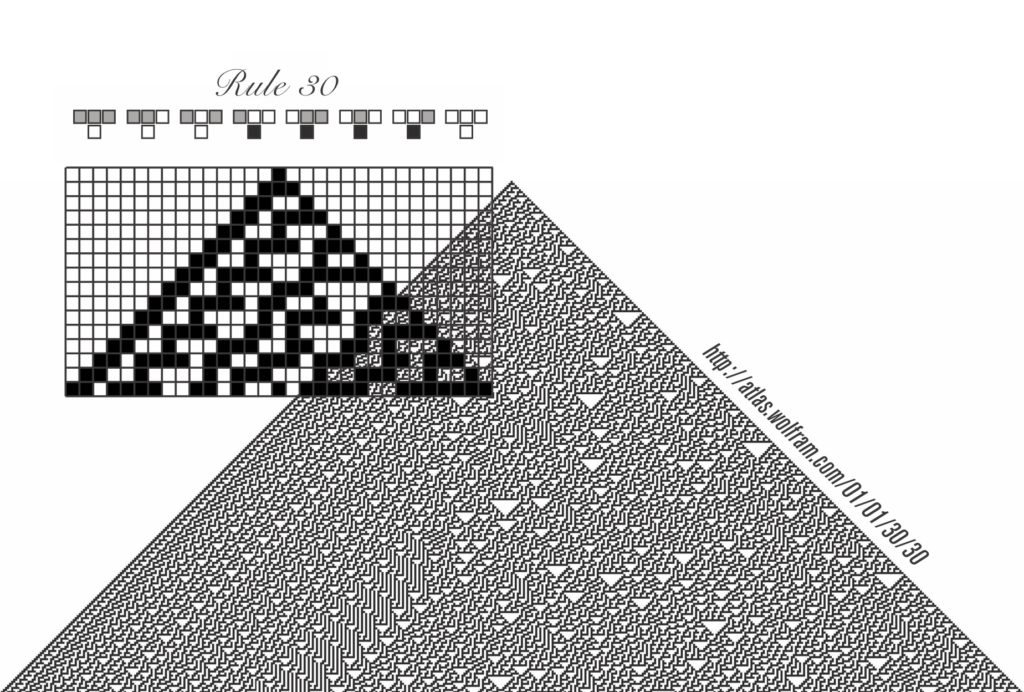
\includegraphics[width=\imsize]{regla30.jpg}
	\caption[ Diagrama que ilustra el patrón generado por la regla 30 del autómata celular (AC) unidimensional.]{  Diagrama que ilustra el patrón generado por la regla 30 del autómata celular (AC)  unidimensional.  Las celdas son coloreadas de acuerdo con su estado anterior en relación a su entorno, asignando tonos más oscuros al estado $1$ y tonos más claros al estado $0$. El eje vertical representa la dimensión temporal, permitiendo visualizar la evolución del patrón a lo largo del tiempo. En la parte superior del diagrama, se presentan las reglas que gobiernan la transición hacia el siguiente estado del autómata, expresadas mediante la fórmula $[\text{celda izquierda} \veebar (\text{celda central} \lor \text{celda derecha})]$. Esta regla específica se denomina Regla $30$ debido a su correspondencia binaria, donde ${00011110}_2$ se representa como el número 30.} \label{fig:regla30}
\end{figure}

\begin{figure}[ht]
	\centering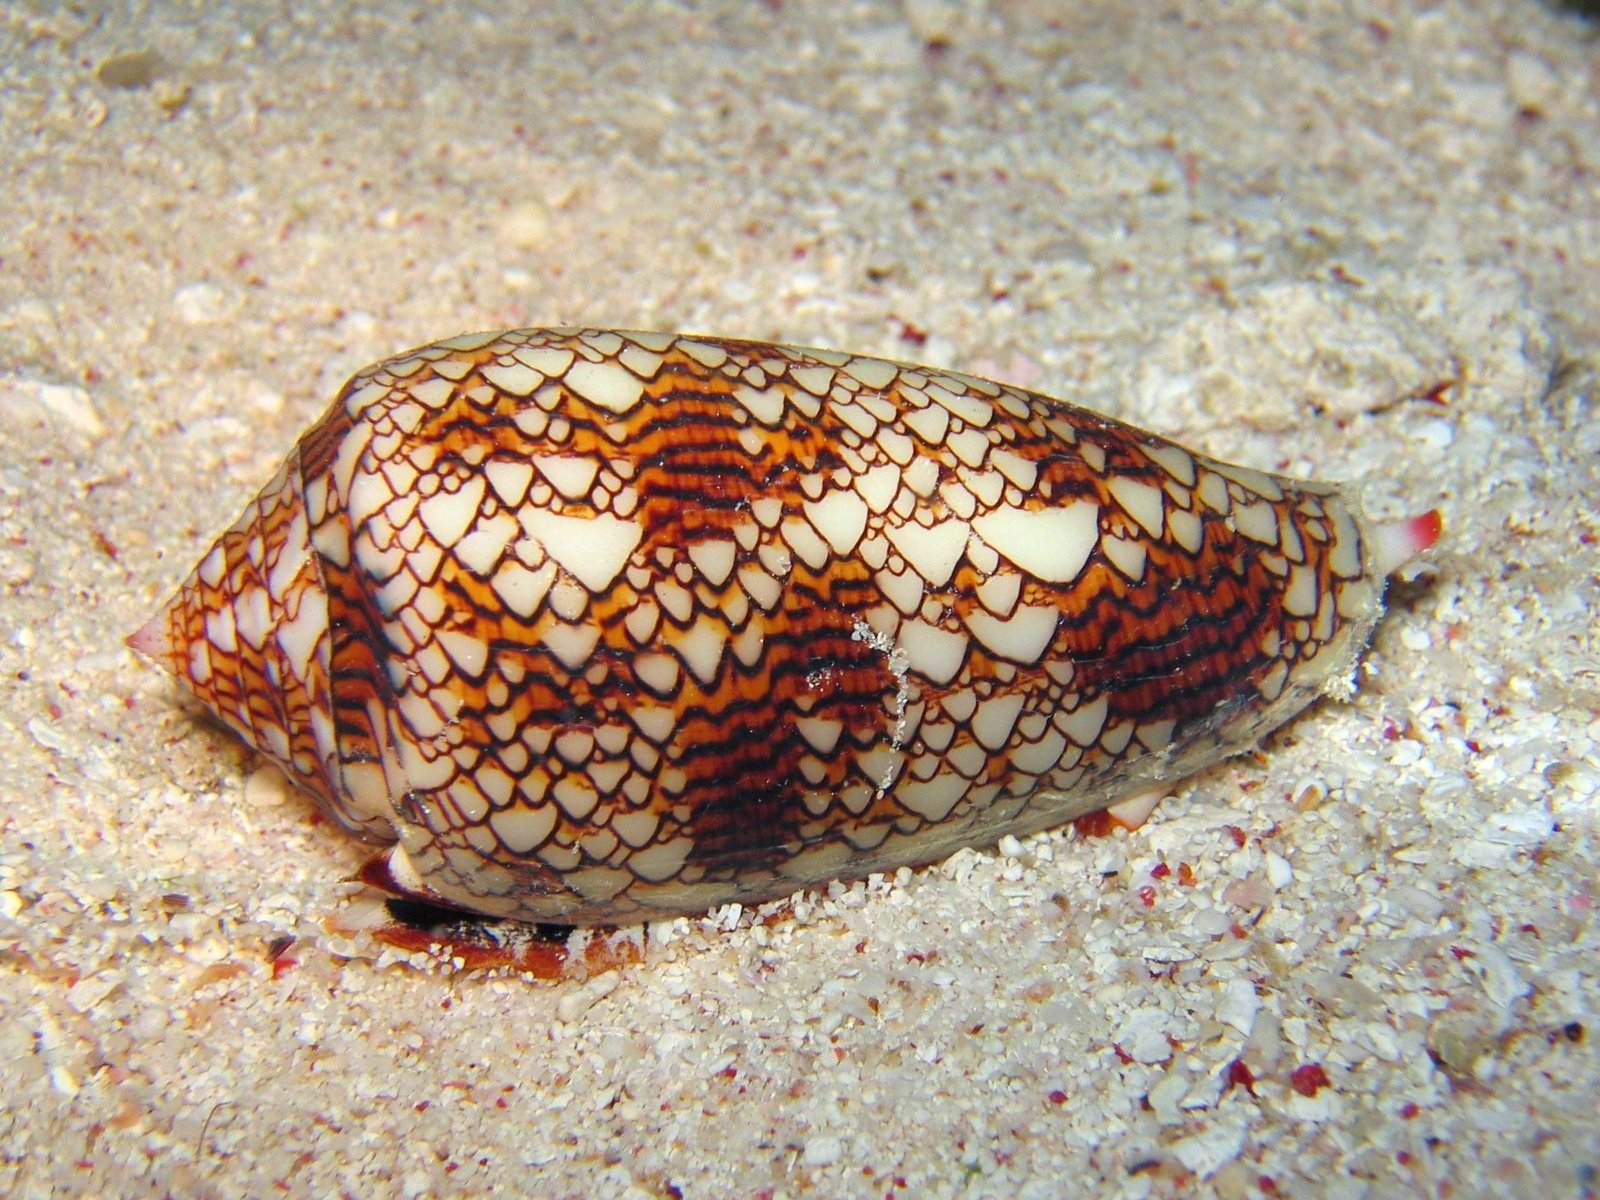
\includegraphics[width=\imsize]{Textile_cone}
	\caption[C Caparazón de Conus textile, una especie presente en las aguas del Indo-Pacífico, que exhibe un patrón de autómata celular con similitudes visuales a la Regla 30.]{ Caparazón de Conus textile, una especie presente en las aguas del Indo-Pacífico, que exhibe un patrón de autómata celular con similitudes visuales a la Regla 30 (Figura adaptada de \protect\cite{ling_english_2005})} \label{fig:conus}
\end{figure}


\subsection{Modelado matemático de autómatas celulares deterministas y estocásticos}\label{sec:SCA}

Los autómatas celulares estocásticos (SCA) pertenecen a la categoría de modelos de red de no equilibrio. Estos modelos se caracterizan por la distribución de celdas (autómatas) en los vértices de una red, donde los enlaces facilitan la interacción y comunicación entre ellas. El análisis de los SCA se centra en los fenómenos que ocurren durante la evolución hacia el equilibrio, así como en aspectos fundamentales como la existencia, número, naturaleza y atracción de las medidas invariantes  de equilibrio \cite{louis_probabilistic_2018}.   En contraste con otras dinámicas asincrónicas, como las ecuaciones diferenciales acopladas o los sistemas de partículas interactuantes, los AC y los SCA pueden definirse directamente en redes infinitas de nodos debido a su naturaleza paralela. Esto evita la necesidad de imponer restricciones a regiones finitas o condiciones adicionales sobre los parámetros para asegurar la existencia del proceso correspondiente. Los AC y SCA se describen mediante el mismo objeto sintáctico, tal como se presenta en la siguiente definición. La distinción entre ellos radica en la forma en que se observa el comportamiento global asociado. Además, los AC deterministas se consideran un caso particular de los SCA. A continuación, se detallan los elementos clave de la configuración matemática de los autómatas:

\begin{itemize}
\item La red  $G$: Se define como un grafo dirigido  $G=(V(G),E(G))$, donde $V(G)$  representa el conjunto de vértices que indican la ubicación de las celdas,  y $E(G)\subseteq V(G)\times V(G)$ es el conjunto de aristas que representan los canales de interacción entre las celdas.
\item El alfabeto $\mathcal{E}$: También conocido como espacio local,, describe los posibles estados o configuraciones que pueden ser adoptados por cada celda. En la mayoría de los autómatas celulares, $\mathcal{E}$ es un conjunto finito con una $\sigma$- álgebra discreta, una topología discreta y una medida uniforme.
\item La vecindad de interacción $\mathcal{N}^I(i)$:  Cada $\mathcal{N}^I(i)\subseteq V(G)$ representa el conjunto de celdas que pueden interactuar con la celda ubicada en $i\in V(G)$. 
\item  El espacio de estado o configuración $\mathcal{S}$:  Representa el estado global de la red de autómatas.   Está equipado con una topología producto y una medida adecuada.  Las configuraciones se denotan como $\mathbf{s}=\left\{s_i:i\in V(G)\right\}$, donde $s_i$ representa el estado de la celda en la ubicación  $i$.
\item Una regla $\mathcal{R}$ que determina la dinámica de los estados de las celdas
\end{itemize}


\subsubsection{Topología de la red y condiciones de contorno}

Los autómatas celulares se definen mediante un grafo $G = (V(G), E(G))$.  El grafo está compuesto por un conjunto $V(G)$ de $N$ nodos (vértices) identificados por el índice $i = 1, \cdots, N$, y un conjunto de aristas $E(G)$ que establecen conexiones entre los nodos, definiendo así la estructura del autómata.  Generalmente, se utiliza un subconjunto finito de la red cuadrada $\mathbb{Z}^2$ como grafo $G$. Esta red cuadrada está compuesta por nodos ubicados en coordenadas enteras en un plano. Los nodos se denominan \textquote{sitios} y la red es invariante ante traslaciones. 

Una arista $(i,j)\in E(G)$ se define como una conexión que tiene origen en el nodo $i$ y destino en el nodo $j$. Se considera una arista saliente de $i$ y entrante en $j$. Decimos que el nodo $i$ es vecino de $j$ si existe una arista entrante de $i$ a $j$, es decir, $(i, j) \in E(G)$. La vecindad de $j$ se define como el conjunto $\mathcal{N}(j) \subseteq V$ que comprende todos los vecinos del nodo $i$.  

\begin{equation}\label{eq:61}
	\mathcal{N}(i)= \left\{j:(i,j)\in E\right\}
\end{equation}

La vecindad también puede ser representada mediante una matriz de adyacencia $\bm{A}$, cuyos elementos están determinados por:

\begin{equation}\label{eq:62}
	a_{ij}=	\begin{cases}
		1, & \text{si} \ \left(i,j\right)\in \mathcal{E}\\
		0, & \text{en caso contrario}
	\end{cases}
\end{equation}

con $i, j = 1,\cdots, N$. Es importante destacar que las conexiones entre nodos pueden ser unidireccionales, lo que significa que no necesariamente son simétricas. Además, es posible tener múltiples redes de conexión entre los mismos nodos, conocidas como multigrafos, representadas mediante diferentes matrices de adyacencia $a_{ij}^{(1)} , a_{ij} ^{(2)}, \cdots$.

Durante los experimentos computacionales en autómatas celulares, se trabaja con redes finitas. Para abordar esta limitación, se establecen condiciones de frontera que determinan la vecindad de las celdas en los bordes de la red. Una estrategia común es la extensión periódica de la red, donde los límites opuestos de la red se conectan. Esto permite que los nodos en los bordes tengan vecinos en el extremo opuesto de la red, creando una estructura anular en una dimensión o un toro en dos dimensiones. Estas condiciones de contorno periódicas se utilizan para aproximar la simulación en una red infinita.  Es importante tener en cuenta que también es posible introducir periodicidades espaciales artificiales en el sistema.

\subsubsection{Vecindario de interacción}

En las redes, se observa una disminución en la fuerza de interacción entre dos nodos a medida que aumenta la distancia en el grafo. Para abordar esta característica, los AC introducen el concepto de vecindad. La vecindad se define como los nodos que están conectados por un número máximo de enlaces, lo cual es crucial en el estudio de los AC, ya que permite evaluar la influencia de los nodos vecinos en el estado de un nodo en particular. En este contexto, se establece el vecindario de interacción $\mathcal{N}^I(i)$ como el conjunto de nodos que afectan el estado del nodo $i$. 

\begin{equation}\label{eq:43}
	\mathcal{N}^I(i) = \left\{j:(i,j)\in E^I\right\}=\left\{j\right\}_{a_{ij}=1}\subseteq G,
\end{equation}

En el caso particular de redes periódicas con condiciones de contorno no periódicas, es necesario considerar la vecindad de interacción en los límites de la red. En las redes bidimensionales cuadradas, se utilizan dos tipos de vecindades comunes: la vecindad de von Neumann y la vecindad de Moore. La vecindad de von Neumann se compone de una celda central y sus cuatro vecinos adyacentes: norte, oeste, sur y este. Por otro lado, la vecindad de Moore incluye los cuatro vecinos adyacentes y los cuatro vecinos diagonales: noreste, noroeste, sureste y suroeste, lo que da un total de nueve celdas.  Estos dos tipos de vecindades estándar se presentan visualmente en la Figura 5.3, proporcionando una representación clara de sus configuraciones en una red bidimensional cuadrada.


\begin{figure}[ht]
	\centering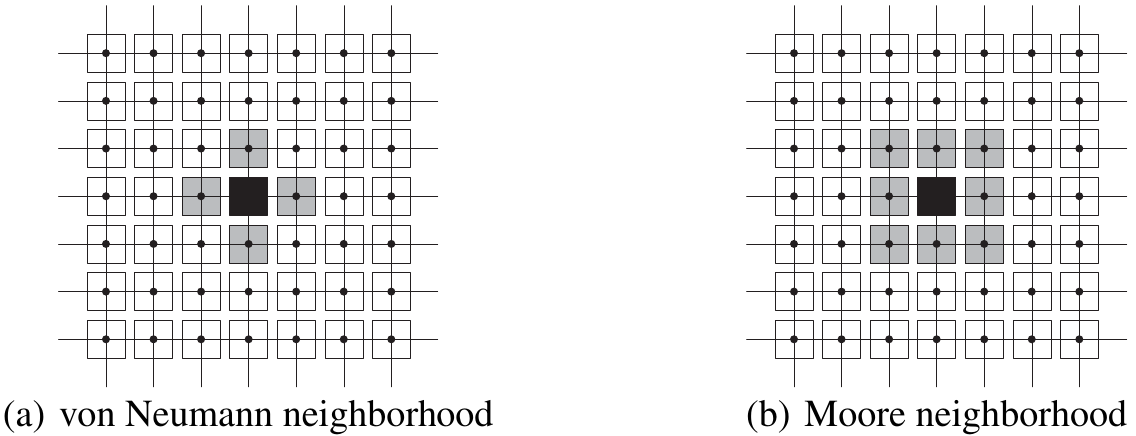
\includegraphics[width=\imsize]{celdas}
	\caption[Ejemplos de vecindades de interacción en una red cuadrada bidimensional. ]{Ejemplos de vecindades de interacción en una red cuadrada bidimensional. Se destacan las celdas grises y negras, que representan los nodos en la red, mientras que la celda negra corresponde al nodo central de interés.} 	\label{fig:celdas}
\end{figure}


\subsubsection{Estados}


Cada nodo $i\in G$ se le asigna un valor de estado $s_i$ tomado de un conjunto finito $\mathcal{E}$ que contiene estados elementales. Esta asignación se define mediante una función de mapeo:

\begin{equation}
	s:G\rightarrow\mathcal{E}.
\end{equation}

El conjunto  $\mathcal{E}$ puede incluir números, símbolos u otros objetos, como células biológicas.  La configuración global del autómata, representada por el vector $\mathbf{s} \in  \mathcal{E}^{N}$, se determina a partir de los valores de estado de todos los nodos en la red, es decir,

\begin{equation}\label{eq:44}
\mathbf{s} \coloneqq \left(s_1,\cdots,s_N\right) = \left(s_i\right)_{i\in G}.
\end{equation}
El espacio de estado $\mathcal{S}$  abarca todas las posibles configuraciones globales y se define como  $\mathcal{S} = \mathcal{E}^{N}$.  Por otro lado, una configuración local se refiere a un vector $\mathbf{s}_\mathcal{M}$   compuesto por los valores de estado de un subconjunto ordenado $\mathcal{M}$   de nodos en la red $G$

\begin{equation}\label{eq:45}
\mathbf{s}_\mathcal{M} \coloneqq \left(s_1,\cdots,s_\mathcal{M}\right)=(s_i)_{i\in\mathcal{M}}, \ \mathcal{M} \subset G.
\end{equation}

La notación $\mathbf{s}\mid\mathcal{M}=\mathbf{s}_\mathcal{M}\in\mathcal{S}\mid\mathcal{M}$  se utiliza para indicar la restricción de la configuración global  $\mathbf{s}$ 
al conjunto $\mathcal{M}$.  Además, la configuración local en relación al entorno de interacción  $\mathcal{N}^I( )\subseteq G$ de un nodo  $i$ se denota como $\mathbf{s}_{\mathcal{N}(i)} \in \mathcal{S}_{\mathcal{N}(i)} \coloneqq \mathcal{S}\mid \mathcal{N}^I(i)$.

\subsection{Dinámica del sistema}\label{sec:dinamica_automata}

La dinámica de un autómata celular está determinada por una regla de transición local, representada por $\mathcal{R}$, que determina el estado futuro de cada nodo en función de su configuración de vecindad de interacción. Formalmente, esta regla se define como:


\begin{align}\label{eq:46}
	\mathcal{R}&:\mathcal{E}^\nu\rightarrow\mathcal{E}, \quad \text{donde} \  \nu = \left| \mathcal{N}_n^I\right|.\\
\end{align}


Donde $ \nu = \left| \mathcal{N}_n^I\right|$ representa la cardinalidad de $\mathcal{N}_n^I$. Se considera que la regla $\mathcal{R}$  es espacialmente homogénea, lo que significa que no depende explícitamente de la posición del nodo $i$. Sin embargo, se pueden introducir variaciones para permitir la falta de homogeneidad espacial y temporal en la regla. Por ejemplo, es posible incorporar reglas dependientes del tiempo, como alternar entre dos reglas en pasos de tiempo pares e impares, tal como se utiliza en modelos de autómatas celulares para casos como la percolación dirigida o la dinámica de espín de Ising. Aunque en general se asume que la regla de transición es espacialmente homogénea.


En un autómata celular determinista, la regla local es determinista y genera un único estado siguiente para cada nodo. Por lo tanto, bajo condiciones iniciales fijas, la evolución futura del autómata es predecible y está determinada de manera única.

Por otro lado, cuando las actualizaciones son aleatorias, se tiene un autómata celular estocástico que sigue un proceso de Markov. En cada paso de tiempo, el estado de cada nodo se actualiza aleatoriamente e independientemente de los demás, siguiendo una distribución de probabilidad que depende del patrón actual de símbolos en una colección finita de sitios vecinos \cite{marcovici_ergodicity_2019}. En un autómata celular estocástico, la regla de transición local se define de la siguiente manera:

\begin{equation}\label{eq:47}
\mathcal{R}\left(\mathbf{s}_{\mathcal{N}(i)}\right) = \begin{cases}
	z^1& \text{con probabilidad} \ W\left(\mathbf{s}_{\mathcal{N}(i)}\rightarrow z^1\right),\\
	\vdots\\
	z^{\left\| \mathcal{E}\right\|} & \text{con probabilidad} \ W\left(\mathbf{s}_{\mathcal{N}(i)}\rightarrow z^{\left\| \mathcal{E}\right\|} \right),
\end{cases}
\end{equation}

donde $z^j \in \mathcal{E} := \left\{z^1,\cdots,z^{\left\|\mathcal{E} \right\| }\right\}$ y $W\left(\mathbf{s}_{\mathcal{N}(i)}\rightarrow z^j\right)$ es la probabilidad de transición independiente del tiempo.  Esta probabilidad indica la posibilidad de que el nodo alcance el estado elemental $z^j$, dada la configuración de vecindad $\mathbf{s}_{\mathcal{N}(i)}$ en ese momento. Es importante destacar que esta probabilidad de transición debe satisfacer ciertas condiciones:

\begin{equation}\label{eq:48}
W:\mathcal{E}^\nu\times\mathcal{E}\rightarrow[0,1] \quad \text{y} \quad  \sum_{j=1}^{\left\| \mathcal{E}\right\| }{W\left(\mathbf{s}_{\mathcal{N}(i)}\rightarrow z^j\right)}=1, \quad \mathbf{s}_{\mathcal{N}(i)}\in\mathcal{E}^\nu,z^j\in\mathcal{E}.
\end{equation}

Es relevante mencionar que cualquier regla local determinista puede considerarse como un caso especial de una regla probabilística, donde la probabilidad de transición es igual a $1$ para el estado objetivo y $0$ para los demás estados, es decir

\begin{equation}\label{eq:49}
	W\left(\mathbf{s}_{\mathcal{N}(i)}\rightarrow z^j\right)=1 \quad \text{y} \quad W\left(\mathbf{s}_{\mathcal{N}(i)}\rightarrow z^l\right)=0 \quad \forall l\neq j,z^j,z^l\in\mathcal{E}.
\end{equation}


Los autómatas celulares estocásticos son una generalización valiosa en el campo de los sistemas complejos, debido a su capacidad para ajustar los parámetros de una regla en un rango continuo de valores, a pesar de la naturaleza discreta inherente a los autómatas celulares.   En un autómata celular con actualización síncrona, la regla local se aplica simultáneamente a cada nodo de la red antes de que los nuevos estados influyan en otros nodos. Esto implica que la dinámica global está determinada por una función global  $\mathcal{R}_g:\mathcal{S}\rightarrow\mathcal{S}$ tal que para cada configuración global $\mathbf{s} \in \mathcal{S}$,

\begin{equation}\label{eq:50}
	\mathcal{R}_g(\mathbf{s}(i))=\mathcal{R}\left(\mathbf{s}_{\mathcal{N}(i)}\right) \quad \forall i\in G.
\end{equation}

En consecuencia, la dinámica global está completamente definida por la regla local $\mathcal{R}$.   Denotamos la configuración global en pasos de tiempo posteriores $t \in \mathbb{N}_0$ como  $\mathbf{s}(t)= (s_1(t),\cdots, s_N( t)) \in \mathcal{S}$, donde $s_i(t) \in \mathcal{E}$ representa el estado del nodo  $i$ en el tiempo $t$.  La configuración local del nodo $i$ en el tiempo $t$  está dada por $\mathbf{s}_{\mathcal{N}(i)} (t) \in  \mathcal{S}_{\mathcal{N} (t)}$.   Para cada configuración global inicial 
 $\mathbf{s} (0) \in \mathcal{S}$ en el tiempo $t=0$,  el desarrollo temporal del sistema se describe mediante la siguiente relación:


\begin{equation}\label{eq:51}
\mathbf{s}(t+1)=\mathcal{R}_g(\mathbf{s}(t)),
\end{equation}

La dinámica de un estado $s_i(t)$ se determina mediante la regla local $\mathcal{R}$,  es decir:
\begin{equation}\label{eq:52}
s_i(t+1)=\mathcal{R}\left(\mathbf{s}_{\mathcal{N}(i)}(t)\right).
\end{equation}

En otras palabras, el estado del nodo $s_i( t )$ depende de los estados anteriores de los nodos de entrada.  Dado que el número de configuraciones posibles es finito para una red finita, cualquier condición inicial eventualmente conduce a un ciclo temporal periódico en un autómata celular determinista. En el caso de los autómatas celulares estocásticos, se puede entender su evolución como una cadena de Markov, donde los elementos de la matriz de transición se obtienen multiplicando las probabilidades de transición locales. La dinámica global de los autómatas celulares finitos se puede visualizar mediante un grafo de transiciones globales, donde cada nodo representa una configuración única del autómata celular y las aristas que los conectan representan las transiciones globales entre las configuraciones.


En extensiones de los modelos de autómatas celulares, se permite la actualización asíncrona y no se limita a vecindarios finitos. En este caso, la regla local se aplica de forma independiente a cada nodo, lo que implica que el nuevo estado de un nodo afecta el cálculo de los estados en celdas vecinas. Estas diferencias en la actualización asíncrona tienen implicaciones significativas en la dinámica y los patrones generados por los autómatas celulares. Se han propuesto y analizado varios algoritmos de actualización asíncrona \cite{schonfisch_synchronous_1999,cornforth_ordered_2005,fates_guided_2013}. Cabe destacar que varios estudios han implementado modelos asíncronos y han observado que su comportamiento difiere de los modelos síncronos. Sin embargo, Nehaniv demostró que es posible emular con precisión el comportamiento de un autómata celular síncrono mediante una sencilla modificación del autómata celular asíncrono utilizando un método general \cite{nehaniv_asynchronous_2011}.



\section{Modelos de AC de sistemas excitables}\label{sec:medios_excitables}

En el apartado \cref{sec:mediosexcitables}  se discute la naturaleza de los medios excitables, los cuales son sistemas extendidos de no equilibrio. Estos sistemas exhiben estados uniformes que son linealmente estables, pero que pueden ser perturbados por estímulos finitos. Los medios excitables consisten en elementos acoplados, cada uno de los cuales muestra una dinámica estable hasta que se alcanza un umbral específico. La evolución de estos elementos en el espacio de fase se manifiesta como ondas viajeras en el tiempo real. La capacidad de respuesta a las perturbaciones es una característica fundamental de los elementos excitables. Cuando se supera un umbral determinado, una perturbación excitará un elemento inactivo, que luego volverá a la inactividad tras un tiempo característico, sin importar la magnitud de la perturbación. Estas ondas excitables ilustran de manera sorprendente la ruptura de simetría espontánea y la organización espacio-temporal en sistemas físicos y químicos.

La investigación experimental y numérica de los sistemas excitables tiene una larga trayectoria. Por lo general, se utiliza un sistema de ecuaciones diferenciales parciales para modelar el mecanismo de reacción-difusión subyacente. Si bien estos modelos suelen ser efectivos, la implementación de métodos numéricos adecuados puede ser compleja y las simulaciones computacionales pueden requerir mucho tiempo, especialmente en el caso de sistemas tridimensionales.

En los últimos años, los modelos basados en autómatas celulares han ganado popularidad como una alternativa para el modelado de dichos sistemas. Estos modelos presentan ventajas significativas, como un menor costo computacional, una mayor flexibilidad y una configuración más sencilla. Los modelos de autómatas celulares para medios excitables buscan simplificar el sistema al máximo, donde cada unidad excitante puede asumir un número finito de estados. La dinámica de actualización de cada unidad excitante depende tanto de su estado actual como del estado de sus vecinos \cite{sinha_patterns_2019}.



En 1946, Wiener y Rosenblueth dieron los primeros pasos hacia la comprensión de los medios biológicos excitables al utilizar autómatas celulares. Su estudio se enfocó en explicar las arritmias cardíacas generadas por las ondas espirales, y propusieron los estados refractario, quiescente y excitado como base para entender el comportamiento de dichos medios \cite{wiener_mathematical_1946}.  Posteriormente, en 1978, Greenberg y Hastings llevaron a cabo un estudio fundamental en el que presentaron un modelo de autómatas celulares con una dinámica trifásica, cíclica y excitante para el modelado de medios excitables. Este modelo, conocido como el modelo de autómatas celulares de Greenberg-Hastings (GHCA) \cite{greenberg_spatial_1978}, ha demostrado ser un marco fructífero para el estudio y análisis de dichos sistemas. En particular, se ha utilizado con éxito para modelar las reacciones de Belousov-Zhabotinsky, que representan un ejemplo prototípico de medios excitables, y ha proporcionado información valiosa sobre estos sistemas. En general, el modelo GHCA pertenece a una clase más amplia de autómatas celulares con dinámica local excitante y cíclica, y se ha implementado en modelos computacionales para estudiar fenómenos biológicos, como los patrones espaciotemporales de los ritmos cardíacos, las ondas cerebrales macroscópicas y los procesos epidémicos  \cite{hadeler_cellular_2017}.



\subsection{Modelo  de Greenberg-Hastings}\label{sec:modeloGH}


El modelo Greenberg-Hastings fue desarrollado por Greenberg y Hastings como una simplificación del modelo Fitzhugh-Nagumo, que describe la excitación nerviosa. Mientras que el modelo Fitzhugh-Nagumo exhibe un comportamiento periódico cuando la entrada dendrítica supera un umbral  (ver \cref{modelo_Fitzhugh-Nagumo}), el modelo Greenberg-Hastings se centra en capturar esta dinámica de manera más simplificada y abstraída. El modelo Fitzhugh-Nagumo se compone de dos ecuaciones diferenciales acopladas, que representan el estado del sistema. En su mayoría, el sistema permanece en las dos partes estables del manifold lento, y los saltos a través del manifold rápido son breves y pueden ser desestimados. Al discretizar el tiempo y analizar la solución de las ecuaciones en puntos de tiempo discretos equidistantes, se observa que la célula sigue una secuencia discreta: primero avanza por la rama activada del manifold lento y luego por la rama refractaria (ver  \Cref{fig:Nagumo}). Se utiliza el estado 0 para denotar el estado de reposo, y los estados se numeran en orden ascendente \cite{hadeler_cellular_2017}. Dentro del manifold lento, encontramos varios estados excitados, que se denominan $K$, junto con $\kappa - K$ estados refractarios. Además, se incluye el estado de reposo, lo que da un total de $\kappa + 1$ estados posibles. Estos estados se recorren de forma cíclica, siguiendo la secuencia:

\begin{equation}
	\underbrace{0}_{\text{quiescente}}\to \underbrace{1\to2\to\cdots K-1\to K}_{\text{excitado}}\to\underbrace{K+1\to K+2\to\cdots \kappa-1\to \kappa}_{\text{refractario}}\to\underbrace{0}_{\text{quiescente}}.
\end{equation}

\begin{figure}[ht]
	\centering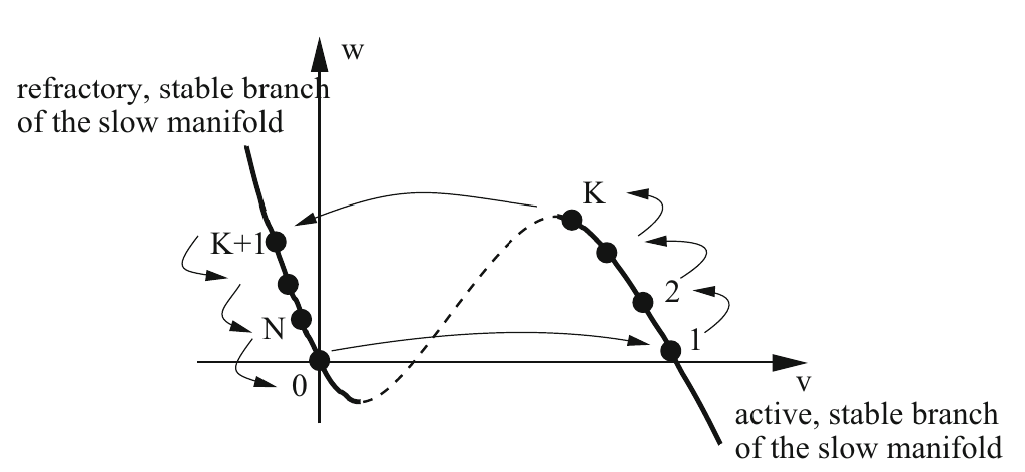
\includegraphics[width=\imsize]{Nagumo.png}
	\caption[Reducción del modelo Fitzhugh-Nagumo a un sistema discreto. ]{Reducción del modelo Fitzhugh-Nagumo a un sistema discreto. El estado sigue la parte excitada y luego la parte refractaria del manifold lento. Utilizando pasos de tiempo discretos, el sistema recorre los estados marcados con puntos negros. (adaptada de \protect\cite{hadeler_cellular_2017})}\label{fig:Nagumo}
\end{figure}

Para proporcionar una descripción completa del modelo, se deben tener en cuenta las siguientes características:

\begin{enumerate}
	\item  Una vez que una celda alcanza el estado $1$, sigue una secuencia determinista de estados ascendentes  $2,\cdots,\kappa$, independientemente de las celdas vecinas. En cada paso de tiempo, el estado se incrementa en uno, hasta que alcanza el estado $\kappa + 1$, que se reduce a $0$ mediante el módulo $\kappa + 1$. El acoplamiento entre las células vecinas es tan débil que solo el estado de reposo puede ser afectado por las células adyacentes.
	\item Si una celda está en estado de reposo, la transición $0\to1$  ocurre cuando al menos $\theta$ celdas en la vecindad de von Neumann se encuentran en un estado excitado $1,\cdots,K$ . 
\end{enumerate}

\begin{definitionT}[Autómata Celular de Greenberg-Hastings]
	Consideremos $G=\mathbb{Z}^2$ como la cuadrícula y $\mathcal{N}_4^I(i)$  como la vecindad de von Neumann. Sean $K,\kappa,\theta, \in \mathbb{N}$, donde $0<K<\kappa$ y  sea $\mathcal{E}=\left\{0,\cdots,\kappa\right\}$.   La dinámica de un estado $s_i(t)$ se describe mediante la siguiente ecuación discreta:
	\begin{align}\label{eq:53}
	s_i(t+1)&= \mathcal{R}(\mathbf{s}_{\mathcal{N}(i)}(t)) \\	
		&=\begin{cases}
			(i+1) \mod (\kappa+1) & \text{si} \ s_i(t)=i\in\mathcal{E}\backslash \left\{0\right\},\\
			0 & \text{si} \ s_i(t)=0 \land \# \left\{ j \in \mathcal{N}^I(i):  1 \leq s_j \leq K\right\}<\theta,\\
			1 & \text{si} \ s_i(t)=0 \land \# \left\{ j \in \mathcal{N}^I(i):  1 \leq s_j \leq K\right\}\geq\theta,
		\end{cases}
	\end{align}
	
	este sistema dinámico discreto se denomina autómata celular de AC de Greenberg-Hastings. 
\end{definitionT}

Este sistema  ha demostrado converger hacia un estado estacionario de oscilaciones espaciotemporales o hacia un punto fijo sin actividad en el sistema.   Para facilitar su análisis, asignamos colores a los $\kappa + 1$ posibles estados en cada celda. La \Cref{fig:gh} muestra ejemplos representativos de la evolución del modelo GHCA en una cuadrícula de tamaño $240\times240$ , con diferentes valores de $\theta$ y $\kappa$. En estos experimentos, partimos de una configuración inicial conocida como \textquote{sopa primordial}, donde los colores iniciales de las celdas son independientes y tienen igual probabilidad de tomar cualquiera de los $\kappa + 1$ valores posibles.


\begin{figure}[h!]
	\centering
	\begin{subfigure}{0.45\linewidth}
		
\includegraphics[width=\linewidth]{gh1} 
		\caption{$\theta=6,\kappa=8$}
		\label{fig:gh1a}
	\end{subfigure}\hfill
	\begin{subfigure}{0.45\linewidth}
		
\includegraphics[width=\linewidth]{gh2}
		\caption{$\theta=7,\kappa=8$}
		\label{fig:gh1b}
	\end{subfigure}
	
	\begin{subfigure}{0.45\linewidth}
		
\includegraphics[width=\linewidth]{gh3}
		\caption{$\theta=9,\kappa=6$}
		\label{fig:gh1c}
	\end{subfigure}\hfill
	\begin{subfigure}{0.45\linewidth}
		
\includegraphics[width=\linewidth]{gh4}
		\caption{$\theta=10,\kappa=5$}
		\label{fig:ghd}
	\end{subfigure}
	\caption[Instantáneas representativas que ilustran la evolución del modelo de Greenberg-Hastings en una cuadrícula de tamaño $240\times240$, con variaciones en los valores de $\theta$ y $\kappa$. ]{Instantáneas representativas que ilustran la evolución del modelo de Greenberg-Hastings en una cuadrícula de tamaño $240\times240$, con variaciones en los valores de $\theta$ y $\kappa$. Los estados iniciales se generaron asignando colores de manera aleatoria a cada celda con la misma probabilidad. Las instantáneas fueron capturadas después de $100$ pasos. Se implementaron condiciones de contorno periódicas para garantizar la consistencia, lo que implica que los bordes opuestos son idénticos (Imágenes obtenidas de \protect\cite{durrett_asymptotic_1993}).}
	\label{fig:gh}
\end{figure}





\section{Dinámica critica en el C elegans}

En el campo de la neurociencia actual, uno de los desafíos más relevantes consiste en comprender cómo surge y se organiza la actividad neuronal compleja a partir de las interacciones entre las neuronas. En los últimos años, se ha prestado mayor atención a este desafío a medida que se han desarrollado y mejorado las técnicas experimentales para registrar simultáneamente la actividad de múltiples neuronas, lo que proporciona conjuntos de datos valiosos para su análisis. Se ha observado que, incluso en ausencia de estímulos externos, la actividad de la red neuronal se organiza en patrones espacio-temporales complejos que reflejan, hasta cierto punto, la arquitectura subyacente de la red. Estos patrones dinámicos muestran similitudes con los sistemas termodinámicos que experimentan una transición de fase de segundo orden, lo que respalda la hipótesis de que el cerebro funciona como un sistema autoorganizado en un estado crítico. Un experimento relevante realizado por Kato et al. combinó tecnologías avanzadas, como la obtención de imágenes de calcio a nivel de una sola célula, para registrar la actividad neuronal en todo el cerebro de un  gusano Caenorhabditis elegans  inmovilizado  en un pequeño canal \cite{kato_global_2015}.  Los resultados obtenidos demostraron una actividad dinámica y coordinada en una amplia proporción de las neuronas cerebrales. Además, Kaplan et al. realizaron experimentos adicionales que confirmaron y ampliaron estos hallazgos  \cite{kaplan_nested_2020}.


Asimismo, es fundamental investigar la relación entre la actividad neuronal y la arquitectura de la red. Estudios previos han demostrado que la complejidad de la arquitectura determina las interacciones complejas entre las diferentes áreas del cerebro \cite{galan_how_2008}. Se ha observado que las conexiones locales densas y las conexiones de largo alcance escasas tienden a generar un comportamiento complejo a gran escala. Sin embargo, la mayoría de estos estudios se han centrado en un nivel macroscópico, describiendo las interacciones entre áreas cerebrales o en el contexto general de arquitecturas de redes complejas pero que no abarca todo el sistema nervioso de forma global, lo que limita su aplicabilidad y generalización.


En esta tesis de doctorado, se propone un enfoque novedoso para abordar estos desafíos, integrando la dinámica neuronal a nivel de sinapsis en una arquitectura que abarque todo el cerebro. Para lograrlo, se utilizará el conectoma completo de ambos sexos de Caenorhabditis elegans. Este enfoque supera las limitaciones de los modelos actuales, que se basan en regiones cerebrales macroscópicas y emplean una dinámica de red basada en un número reducido de neuronas. Además, al aprovechar las diferencias en el sistema nervioso entre los sexos de Caenorhabditis elegans, será posible investigar la relación entre la arquitectura de la red y la actividad espontánea a nivel global.  Para abordar este problema, se empleará un enfoque de modelado estocástico, ampliamente utilizado en la neurociencia matemática. La actividad neuronal presenta un carácter estocástico, por lo que la interacción entre la excitabilidad neuronal y el estocasticismo constituye un aspecto central en esta investigación. En ausencia de estímulos externos, la red neuronal estará influenciada por fluctuaciones intrínsecas y aleatorias, modeladas como actividad espontanea. Estas fluctuaciones surgirán de las variaciones en los eventos de apertura y cierre de los canales iónicos, así como de la liberación sináptica espontánea y otras fuentes de variabilidad biológica. Estas corrientes aleatorias desencadenarán tasas moderadas de activación en las neuronas individuales, las cuales se propagarán a través de la red neuronal gracias a las interacciones sinápticas.





\subsection{Modelo de dinámica neuronal estocástica en el cerebro de C. elegans }\label{sec:modelocritico}


En esta sección, se abordará la construcción de un modelo de red neuronal basado en autómatas celulares estocásticos para simular el comportamiento de las neuronas de disparo. Con el fin de lograr una representación adecuada de la dinámica real de estas neuronas, es crucial comprender  su fisiología, lo que permitirá desarrollar un modelo más realista. Por lo tanto, se iniciará este estudio profundizando en la fisiología de las neuronas de disparo, centrándonos en los detalles del potencial de acción, tal como se muestra en la \cref{fig:spikeautomata}.   Previo a esta sección, se estableció en el \cref{sec:modelo_dinamica_neuronal} que las neuronas de disparo pueden clasificarse en tres estados principales: el estado quiescente, corresponde al período de reposo, en el cual el potencial de membrana neuronal se mantiene estable en a \qty{-70}{\milli\volt}; el estado excitado, cuando el potencial de membrana se eleva desde un umbral de alrededor de \qty{-55}{\milli\volt} hasta \qty{40}{\milli\volt} (potencial de inversión del sodio), para luego retornar a  \qty{-80}{\milli\volt} (potencial de inversión del potasio) en aproximadamente  \qty{1}{\milli\second}; Por último, el estado refractario se caracteriza por el retorno gradual del potencial de membrana hacia el estado de reposo. Con base en los argumentos expuestos en el \cref{sec:modeloGH}, se representa estos estados mediante una variable de estado discreta,  $\mathbf{s} = \{Q, E, R\}$. En esta notación,  $s_i = Q$ representa el estado quiescente, $s_i = E$ el estado excitado y $s_i = R$ corresponde al período refractario. Es importante destacar que la neurona puede disparar únicamente en el estado quiescente ($s_i = Q$), no durante el período refractario. Por lo tanto, se deben considerar tres transiciones de estado: $Q\to E$ , que depende de las conexiones que esta neurona tenga con otras, y $E\to R$, $R\to Q$, que corresponden a decaimientos simples.



\begin{figure}[ht]
	\centering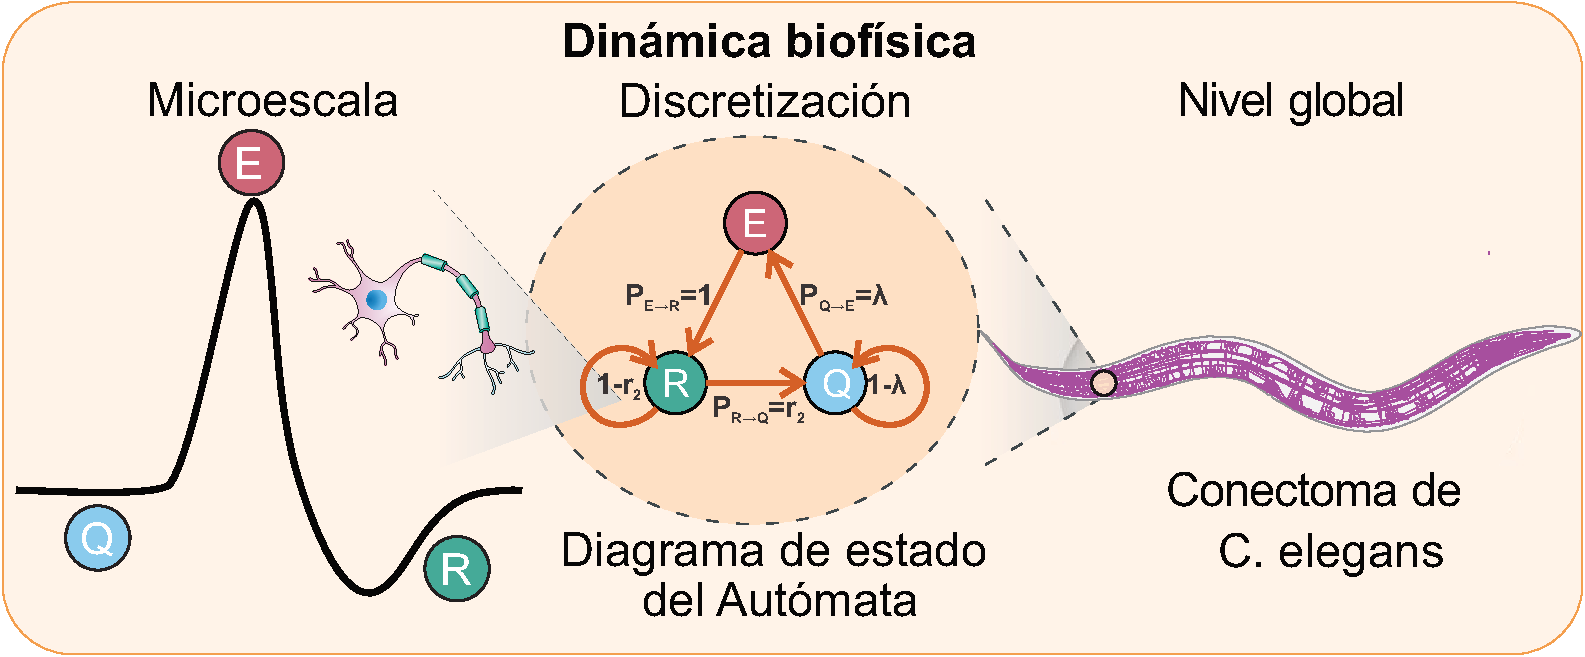
\includegraphics[width=\imsize]{modelo}
	\caption[Modelado de la función de la red cerebral.]{ Modelado de la función de la red cerebral. En el panel izquierdo, se presenta el esquema del potencial de acción de una neurona real, el cual sirve como fundamento del modelo neural. En el panel central, se exhibe el diagrama de estados de los autómatas finitos que representan a las neuronas en el modelo. Estos autómatas pueden adoptar tres estados diferentes: quiescente (Q), excitado (E) o refractario (R). La discretización del potencial de acción, explicada previamente, es esencial para definir estos estados. Las neuronas activas (E; en rojo) emiten ráfagas de potenciales de acción antes de ingresar al estado refractario (R; en verde) durante un período determinado por la probabilidad de $1-r_2$, donde $r_2$ representa la probabilidad de que una neurona pase al estado quiescente. Por otro lado, las neuronas quiescentes (Q; en azul) también desempeñan un papel significativo. Pueden generar potenciales de acción espontáneamente con una probabilidad $r_1$, o ser reclutadas en una ola de actividad por otras neuronas activas si la suma de sus pesos supera un umbral $T$. La probabilidad de esta reclutación, representada en el diagrama de estados mediante el parámetro $\lambda=1-\left[1-r_1\right]\left[1-\Theta\left(\sum_{j=1}^{k_{in,i}}W_{ji}\delta_{s_j,1}-T\right)\right]$, es esencial para la dinámica del modelo y se basa en las características específicas de cada estado neuronal. Para simular la actividad a gran escala del cerebro completo, los autómatas se incorporan al conectoma del C. elegans, lo que permite la aparición de interacciones complejas entre las neuronas y da lugar a una dinámica global compleja, ilustrada en el panel derecho. Cada una de estas neuronas sigue la dinámica presentada en el diagrama de estados y contribuye al comportamiento del modelo a gran escala (La figura ha sido adaptada de las referencias \cite{lynn_physics_2019, jjfroehlich_english_2022}).}\label{fig:spikeautomata}
\end{figure}


Para representar esta abstracción discreta de la fisiología de las neuronas de disparo, se adaptará el modelo computacional del autómata celular de Greenberg-Hastings descrito en el \cref{sec:modeloGH}. En este estudio, se seguirá de cerca la implementación propuesta por \cite{haimovici_brain_2013}.  Las conexiones en el modelo se basarán en la matriz de adjacencia del conectoma del C. elegans, tanto para los sexos hermafrodita como macho, construida por Cook et al \cite{cook_whole-animal_2019}. Para obtener una descripción detallada del conectoma y su derivación a partir de la microscopía electrónica en serie, se puede consultar el apartado 1.1. En resumen, el conectoma del hermafrodita consta de 460 nodos (302 neuronas, 132 músculos y 26 órganos terminales no musculares), mientras que el conectoma del macho cuenta con 579 nodos (385 neuronas, 155 músculos y 39 órganos terminales no musculares). Dichos conectomas presentan un total de 4,887 conexiones químicas (o dirigidas) y 1,447 conexiones gap junction (o no dirigidas) en el caso del hermafrodita, y 5,315 conexiones químicas y 1,755 conexiones gap junction en el caso del macho. Los pesos de estas conexiones, denotados como wij, corresponden al número total de secciones seriales de conectividad EM, teniendo en cuenta tanto el número como el tamaño de las sinapsis. Cabe mencionar que este modelo se limitará únicamente a las conexiones químicas del conectoma, ya que nuestro objetivo es enfocarnos exclusivamente en las sinapsis entre neuronas. Sin embargo, es importante destacar que el modelo es lo suficientemente flexible como para incorporar fácilmente las conexiones eléctricas si se desea (ver, por ejemplo, \cite{protachevicz_how_2018}).

Además de las conexiones, el modelo también tendrá en cuenta otros aspectos relevantes desde el punto de vista neurofisiológico, que pueden tener implicaciones dinámicas significativas.  Entre ellos, se destaca la incorporación de una probabilidad de excitación espontánea $r_1$ en cada neurona, lo que implica que existe una pequeña posibilidad de que una neurona dispare en ausencia total de estímulos externos. Esta excitación espontánea está asociada al ruido neuronal, que proviene de diversas fuentes \cref{table:ruido_neuronas}), como la liberación aleatoria de neurotransmisores en las sinapsis, la activación aleatoria de canales iónicos y, especialmente, la entrada sináptica aleatoria proveniente de otras neuronas.  Para un análisis más detallado del ruido en los sistemas neuronales, se recomienda consultar \cite{faisal_noise_2008,destexhe_neuronal_2012}.  Estudios anteriores han demostrado que un nivel moderado de ruido puede tener efectos beneficiosos en la organización y actividad de los sistemas neuronales \cite{lindner_effects_2004,gosak_spatial_2007,vigelius_stochastic_2012}.

Con toda la información presentada, se procederá a construir el modelo de dinámica neuronal en el conectoma del C. elegans utilizando un autómata celular estocástico, siguiendo el formalismo matemático descrito en el \cref{sec:SCA}.


		

\begin{table}[h!]
	\centering
	\caption[Diversas fuentes de ruido en el sistema nervioso.]{ Diversas fuentes de ruido en el sistema nervioso, adaptada de A. Aldo Faisal et al. \protect{\cite{faisal_noise_2008}}.}
	\begin{tblr}{colspec={X[1,l]X[2,l]},
			row{odd} = {bg=gray8},
			row{even} = {bg=gray9},
			row{1} = {bg=red3, fg=white, font=\sffamily},
		}
		Fuente del ruido neuronal	& Descripción	  \\
		
		Ruido sensorial &   Los estímulos sensoriales externos exhiben intrínsecamente un nivel de ruido debido a su naturaleza termodinámica o mecano-cuántica.\\
		
		Ruido celular &  En cada neurona se acumula ruido debido a la aleatoriedad presente en los procesos celulares encargados del procesamiento de información. Esta variabilidad puede amplificarse aún más como resultado de cálculos no lineales e interacciones en la red neuronal. A nivel bioquímico y biofísico, se desencadenan múltiples procesos estocásticos en las neuronas, entre ellos la síntesis y degradación de proteínas, la apertura y cierre de canales iónicos, la fusión de vesículas sinápticas, así como la difusión y unión de moléculas de señalización a receptores.\\
		
		
		{Ruido eléctrico y \\ potenciales de acción} &   La actividad eléctrica en las neuronas provoca fluctuaciones en el potencial de membrana, incluso en ausencia de entradas sinápticas. El ruido eléctrico, generado por la apertura y cierre aleatorios de los canales iónicos activados por voltaje o ligando, constituye la fuente principal de estas variaciones. \\
		 
		Ruido sináptico &  El ruido sináptico se manifiesta mediante corrientes diminutas (mPSC) que surgen de la liberación espontánea de una o más vesículas neurotransmisoras por las terminales presinápticas. Estas corrientes sinápticas evidencian la naturaleza cuántica de la transmisión sináptica.\\
		
		Ruido  motor &  Este tipo de ruido se atribuye a la variabilidad inherente en los comandos motores (espinales), originada tanto por el ruido presente en las neuronas motoras como por otras fuentes de variabilidad en los músculos y otros elementos relacionados.\\	
	\end{tblr}
	\label{table:ruido_neuronas}
\end{table}



\begin{definitionT}[Modelo estocástico de autómata celular para la dinámica neuronal en C. elegans]
		
Sea $G=(V(G), E(G))$ una red  que  representa el conectoma del C. elegans, donde $V(G)$ y $E(G)$ corresponden al conjunto de nodos y aristas, respectivamente. Cada nodo $i$ (etiquetado como $i = 1, 2, \cdots, N$) en esta red representa una neurona, mientras que las aristas representan las conexiones sinápticas entre ellas (ver Figura 1). Cada neurona $i$ en la red tiene un estado dinámico $s_i(t) \in \mathcal{E} = \{Q, E, R\}$, que describe su actividad en un tiempo $t$ dado.  Específicamente, cada nodo puede encontrarse en uno de los tres estados: quiescente ($Q$), indicando inactividad pero con capacidad de excitación; excitado ($E$), correspondiente al estado de disparo; o refractario ($R$), denotando la incapacidad para disparar.  Se utilizará  una codificación numérica para estos estados: $s_i = 0$ para el estado quiescente, $s_i = 1$ para el estado excitado y $s_i = 0.5$ para el estado refractario.
	
La estructura de la red está completamente descrita por una matriz de adyacencia ponderada $\bm{A} = \{a_{i,j}\}$ de tamaño $N\times N$.  Los elementos no nulos en $\bm{A}$ indican las conexiones entre neuronas, con pesos $w_{ij} \geq 0$ que representan la fuerza de las conexiones. Tanto la conectividad como los pesos son constantes en el tiempo, lo que implica que el conectoma es estático (consideramos un régimen de desorden templado).
	
	
La configuración global de la red en un momento $t$ se expresa mediante el vector $\mathbf{s}(t)\in\mathcal{S}$, de longitud $N$, donde $\mathbf{s}(t) = (s_1(t), s_2(t), \cdots, s_N(t))$. El espacio de estados $\mathcal{S} = \left\{Q,E,R\right\}^N$ abarca todas las combinaciones posibles de estados de las neuronas. La evolución de cada nodo ocurre en tiempo de máquina y su estado en el siguiente instante depende del estado actual de las neuronas que la regulan. Bajo la suposición de que los tiempos característicos de transición son similares para todas las neuronas, estas se actualizan de manera sincrónica en cada paso de tiempo.  Para una configuración global inicial $\mathbf{s}(t = 0) \in \mathcal{S}$, el desarrollo temporal del sistema está determinado por la regla de actualización $\mathbf{s}(t + 1) = \mathcal{R}_g(\mathbf{s}(t))$, donde la dinámica del estado $s_i(t)$ de una neurona $i$ evoluciona según las siguientes reglas:
	
\begin{enumerate}[label=(\roman*)]
\item Si la neurona $i$ se encuentra en estado excitado en el tiempo $t$ ($s_i(t) = E$), entonces en el siguiente paso temporal estará en estado refractario ($s_i(t + 1) = R$).
\item Si la neurona $i$ se encuentra en estado refractario en el tiempo $t$  ($s_i(t) = R$), entonces en el siguiente paso temporal estará en estado quiescente ($s_i(t + 1) = Q$) con una probabilidad fija $r_2$ .  En caso contrario, la neurona permanecerá en estado refractario con una probabilidad de $1 - r_2$.
\item Si la neurona $i$ se encuentra en estado quiescente en el tiempo   $t$  ($s_i(t) = Q$), entonces en el siguiente paso temporal estará en estado excitado ($s_i(t + 1) = E$) si la suma ponderada de los pesos de las conexiones provenientes de las neuronas vecinas activas supera un umbral $T$, es decir, $\sum_j w_{ji}\delta_{s_j(t),E}>T$ (ver \Cref{fig:reglaautomata}). En caso contrario, la neurona aún tiene la posibilidad de transicionar al estado excitado con una probabilidad fija $r_1$. De lo contrario, permanecerá en estado quiescente ($s_i(t + 1) = Q)$.

\end{enumerate}	
	
La evolución dinámica de la red se puede modelar como un proceso de Markov de tiempo discreto, en el cual todas las neuronas se actualizan simultáneamente. En términos matemáticos, la dinámica de cada neurona en la red puede ser formalizada de la siguiente manera:

\begin{equation}
	s_i(t+1)=\mathcal{R}(\mathbf{s}_{\mathcal{N}(i)}(t))=\begin{cases}
 	R& \left\{\begin{aligned}
 		  \text{si}  & \  s_i(t)=E &\  \text{con probabilidad} & \ W(E\to R)  \\
 		\text{si}  &\   s_i(t)=R   & \ \text{con probabilidad}  &\  1-W(R\to Q)
 	\end{aligned}\right.\\
	 	Q & \left\{\begin{aligned}
		\text{si}  & \  s_i(t)=R &\  \text{con probabilidad} & \ W(R\to Q)  \\
		\text{si}  &\   s_i(t)=Q   & \ \text{con probabilidad}  &\  1-W(Q\to E)
	\end{aligned}\right.\\	
		E & \left.\begin{aligned}
		\ \ \text{si}  & \  s_i(t)=Q &\  \text{con probabilidad} & \ W(Q\to E)  \\
	\end{aligned}\right.\\
	\end{cases}
\end{equation}

Donde las probabilidades de transición $W(\tilde{s}_i\to s_i)$ se calculan en el tiempo $t$ y se define como:

\begin{align}\label{eq:55}
	W(E\to R)&=1,\\
	W(R\to Q)&=r_2,\\
	W(Q\to E) &= 1-\left[1-r_1\right]\left[1-\Theta\left(\sum_{j=1}^{k_{in,i}}W_{ji}\delta_{s_j,1}-T\right)\right],\\
\end{align}

La probabilidad $W(\tilde{s}_i\to s_i)$  indica la probabilidad de que la neurona $i$ transicione del estado $\tilde{s}_i$ al estado $s_i$ en el tiempo $t + 1$. La suma se realiza sobre todas las neuronas $j$ que se conectan a la neurona $i$, y $k_{in,i}$ denota el grado de entrada de la neurona $i$.  La función escalón de Heaviside $\Theta(x)$ se define como  $\Theta(x)=1$ si $x \geq 0$, y $0$ en caso contrario. Además, $\delta_{i,j}$ representa la delta de Kronecker. Los parámetros $r_1$ y $r_2$ son números aleatorios independientes extraídos de una distribución uniforme en el intervalo $[0, 1]$. Es importante destacar que los parámetros $r_1$, $r_2$ y $T$ son los mismos para todas las neuronas en este modelo.
\end{definitionT}



\begin{figure}[ht]
	\centering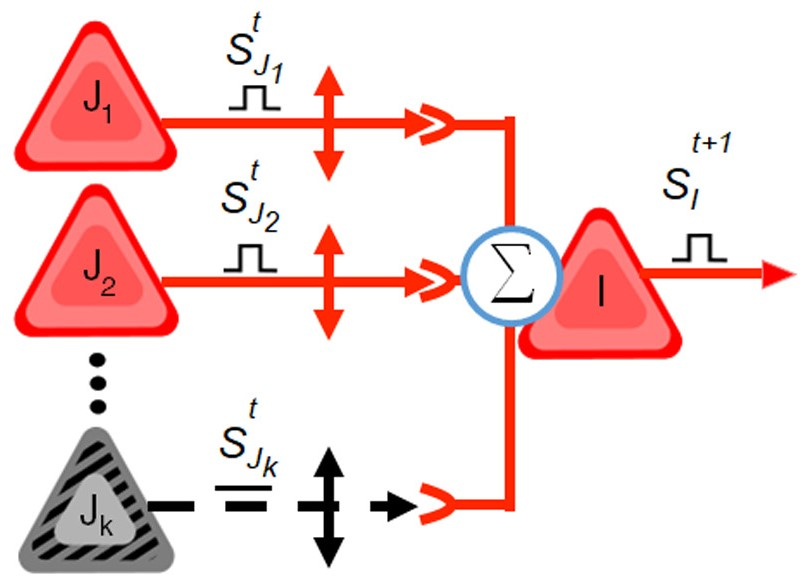
\includegraphics[width=\imsize]{reglaautomata}
	\caption[Regla para la propagación de la actividad neuronal en el modelo GH.]{Regla para la propagación de la actividad neuronal en el modelo GH. En este modelo, la activación de la neurona $i$ en el tiempo $t + 1$ está determinada por una suma ponderada de las contribuciones de todas las neuronas presinápticas activas, denotadas por $j_1$ y $j_2$, y multiplicadas por sus respectivas interacciones sinápticas $w_{ji}$. Esta suma ponderada debe superar el umbral $T$ para que la neurona $i$ se active en el siguiente paso de tiempo. Este proceso de actualización se repite para todas las neuronas inactivas $i$ en cada paso de tiempo. La Figura utiliza triángulos para representar las neuronas y líneas para indicar las interacciones sinápticas entre ellas. Las neuronas activas se muestran en color rojo, mientras que las neuronas inactivas se representan con triángulos grises punteados, tanto en el tiempo $t$ como en $t + 1$. Es importante resaltar que el término de suma en la regla de actualización refleja que el estado de la neurona $i$ en el tiempo $t + 1$ depende de la suma de las contribuciones de las neuronas $j_1$ a $j_n$.} 	\label{fig:reglaautomata}
\end{figure}



Por lo tanto,  las neuronas siempre exhiben un período refractario después de su activación, mientras que las neuronas en estado refractario tienen una probabilidad $r_2$ de retornar al estado quiescente en el siguiente intervalo de tiempo. La probabilidad de activación de una neurona en estado quiescente se define como el complemento del producto de las probabilidades de no activación a través de los distintos mecanismos \cite{diaz_similar_2021}. Un ejemplo de dos pasos de transición consecutivos se esquematiza en la \Cref{fig:modelopasos}. El modelo considera dos mecanismos de excitación: la excitación espontánea, que ocurre con una probabilidad $r_1$ y ejerce un papel de ruido en el sistema, y la excitación transmitida, que se produce de manera determinista.  En particular, una neurona se activará únicamente si se encuentra en estado quiescente y la suma de los pesos de las conexiones con sus vecinos activos supera el umbral $T$ (ver  \Cref{fig:modelopasos}). Los pesos $w_{ij}$ representan la distribución de pesos en el conectoma del C. elegans. Es importante destacar que el estado de cada neurona se actualiza una vez completada la actualización de toda la red.  Durante la dinámica temporal, la activación de una neurona ocurre con mayor frecuencia cuando la excitación entrante proveniente de sus vecinos activos más cercanos excede el umbral fijo $T$. En otras palabras, $T$ funciona como un parámetro umbral que regula la propagación de la actividad excitatoria entrante, de manera similar al potencial de acción en los modelos de neuronas de disparo \cite{rocha_homeostatic_2018}. Por otro lado, los parámetros $r_1$ y $r_2$ controlan la escala temporal de autoactivación y recuperación del estado excitado, respectivamente. Estos parámetros se ajustan en función del tamaño de la red, mientras que $T$ se establece como el parámetro de control del modelo.


\begin{figure}[ht]
	\centering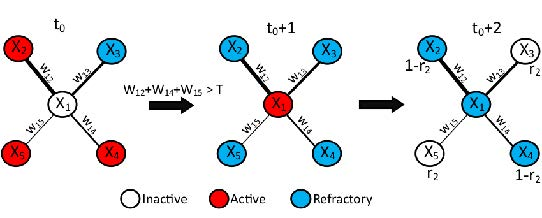
\includegraphics[width=\imsize]{modelopasos}
	\caption[Ejemplo de transiciones dinámicas en el modelo.]{Ejemplo de transiciones dinámicas en el modelo: en $t = t_0$ las neuronas activas son $x_2$,$x_4$ y $x_5$, que excitan $x_1$ en $t = t_0 + 1$, y luego ingresan al estado refractario con $t = t_0 + 2$, $x_3$ y $x_5$ se han recuperado y son susceptibles de excitarse nuevamente,
		mientras que $x_2$ y $x_4$ siguen siendo refractarios.} 	\label{fig:modelopasos}
\end{figure}




\subsection{Teoría de campo medio del modelo neuronal}

En sistemas reales, así como en autómatas celulares estocásticos, se busca comúnmente el estado de equilibrio promediado en el tiempo después de que hayan ocurrido los procesos iniciales rápidos, incluso en presencia de ciclos o aleatoriedad. En esta sección, se analiza el sistema neuronal del modelo previamente presentado que posee múltiples grados de libertad, utilizando herramientas de la mecánica estadística del equilibrio. Estas herramientas permiten describir directamente el estado de equilibrio del sistema en lugar de su evolución temporal. Aunque encontrar una solución exacta para este estado de equilibrio puede ser sumamente difícil e incluso imposible en muchos casos, se hará hincapié en una técnica de aproximación poderosa conocida como aproximación del campo medio, utilizada para describir sistemas con múltiples componentes que interactúan entre sí. La idea detrás de esta aproximación es considerar un solo elemento del sistema influenciado de manera promedio por el resto del sistema, y para lograrlo de manera correcta, es crucial calcular este promedio de manera autoconsistente \cite{bar-yam_dynamics_2003}.

Comenzando con la definición de la probabilidad de que una neurona se encuentre en un estado elemental específico $z^j \in \mathcal{E}=\left\{Q,E,R\right\}$  en el tiempo $t+1$   , podemos expresar esta probabilidad como:

\begin{equation}\label{eq:67}
	P\left(\xi_i(t+1)=z^j\right)=\sum_{\tilde{\mathbf{s}}_{\mathcal{N}(i)}\in\mathcal{S}_{\mathcal{N}(i)}}{P_t(\tilde{\mathbf{s}}_{\mathcal{N}(i)})}\prod_{i\in G}  {p_i\left(\xi_i(t+1)=z^j \mid  \bm{\xi}(t)\mid  \mathcal{N}^I(i) = \tilde{\mathbf{s}}\mid \mathcal{N}^I(i)   \right)}.	
\end{equation}

Al expresar la  \cref{eq:67}  en términos de la probabilidad de que la neurona $i$ esté excitada ($p_i^t \coloneqq  P_t(\tilde{s}=E)$),  en estado quiescente ($q_i^t \coloneqq  P_t(\tilde{s}=Q)$),  o en estado refractario ($r_i^t \coloneqq  P_t(\tilde{s}=R) =1-p_i^t-q_i^t$), se obtienen las siguientes ecuaciones:


\begin{align}
p_i^{t+1}&=q_i^t\left[r_1+\left(1-r_1\right)\Theta\left(\sum_{j=1}^{N}W_{ji}p_j^t-T\right)\right], \label{eq:56}\\
q_i^{t+1}&=q_i^t+r_2\left(1-p_i^t-q_i^t\right)-p_i^{t+1} \label{eq:57},
\end{align}

La \cref{eq:56} se deduce al considerar que  $q_i^t=1-p_i^t$, lo cual representa la probabilidad de que la neurona $i$ esté en estado quiescente en el momento $t$. El término entre paréntesis representa la probabilidad de que la neurona haga una transición al estado excitado, asumiendo que los sucesos en los que los vecinos de la neurona $i$ están excitados en el momento  $t$ son estadísticamente independientes.  Esta aproximación ha demostrado ser efectiva incluso en redes con bucles cortos significativos \cite{rocha_homeostatic_2018,larremore_predicting_2011}.


\subsubsection{Predicción de campo medio del punto crítico}

Pasemos ahora a la predicción del punto crítico mediante el campo medio. Obtener soluciones analíticas para  $p_i^t$ y $q_i^t$ en  las \cref{eq:56,eq:57} es difícil. Sin embargo, estudiando la solución de estado estacionario  ( $t \to\infty$ ) de la aproximación del campo medio, podemos encontrar una solución aproximada para el punto crítico $T_c$.  Para utilizar la aproximación del campo medio, seleccionamos una neurona particular $i$  y hallamos el campo efectivo (o campo medio) al que está expuesta.  Este campo se obtiene sustituyendo todas las variables por sus valores medios. Al establecer  $p_i^t = \left\langle p_i \right\rangle_t   = \bar{p}$ y $q_i^t =\left\langle q_i\right\rangle_t = \bar{q}$ en las ecuaciones \cref{eq:56,eq:57}, donde $\left\langle \cdot \right\rangle_t$ denota el valor esperado en el tiempo, y aproximando $W_i \coloneqq \sum_j W_{ji} \approx \left\langle W \right\rangle$,  con $\left\langle W \right\rangle = \sum_i W_i/N$ como la fuerza media de la red, obtenemos:
 

\begin{align}
	\bar{p}&=\bar{q}\left[r_1+\left(1-r_1\right)\Theta\left(\left< W\right>\bar{p}-T\right)\right], \label{eq:76}\\
	\bar{q}&=\bar{q}+r_2\left(1-\bar{p}-\bar{q}\right)-\bar{p} \label{eq:77},
\end{align}

Considerando la función Heaviside \[\left(\left< W\right>\bar{p}-T\right) = \begin{cases}
	1 & \text{si} T\leq T_c\\
	0 & \text{si } T>T_c
\end{cases}\] y $T_c=\left< W\right>\bar{p}$ como el valor del punto crítico, tras algunas manipulaciones se obtiene:

\begin{equation}\label{eq:78}
	\begin{aligned}
		T_c &= \left\langle W\right\rangle p_{-} =\frac{r_2 }{1+2r_2}\left\langle W\right\rangle ,	\\
		\bar{p}&=\bar{q}=\frac{r_2}{1+2r_2} \eqqcolon p_{-} &\ \text{cuando} \ T<T_c \\
		\bar{p} &= r_1\bar{q} = \frac{r_1r_2}{r_1+r_2+r_1r_2}\eqqcolon p_{+} &\ \text{cuando} \ T>T_c\\
		\end{aligned}
\end{equation}

como era de esperar, $p_{+} < p_{-}$, lo que implica que la actividad es alta cuando el umbral es bajo. Esta expresión es solo una aproximación del umbral crítico exacto. Sin embargo, la solución del campo medio proporciona un resultado razonable al considerar la variabilidad de los puntos críticos con la fuerza de la red  $\left\langle W \right\rangle$, como se ha observado numéricamente. Cabe destacar que $T_c$ depende del sistema nervioso considerado, ya que  $\left\langle W \right\rangle$ varía entre distintos sistemas nerviosos.





de tres estados.  A , q , y  R representan estados activos, inactivos y refractarios, respectivamente. Las flechas representan posibles transiciones con las tasas de transición indicadas. Las flechas abiertas indican que la tasa correspondiente es potencialmente dependiente del estado de la red, es decir, la actividad de las otras neuronas en la red, con funciones de tasa de activación  F y  g.
.

Ahora consideramos el modelo de campo neural con tres estados como un modelo genérico de una neurona en pico (\Cref{fig:estadoneuronas}), donde una neurona puede estar en un estado de pico activo (A), refractario (R) o inactivo (Q). Suponemos que las neuronas pueden sufrir las siguientes cuatro transiciones:


\begin{figure}[ht]
	\centering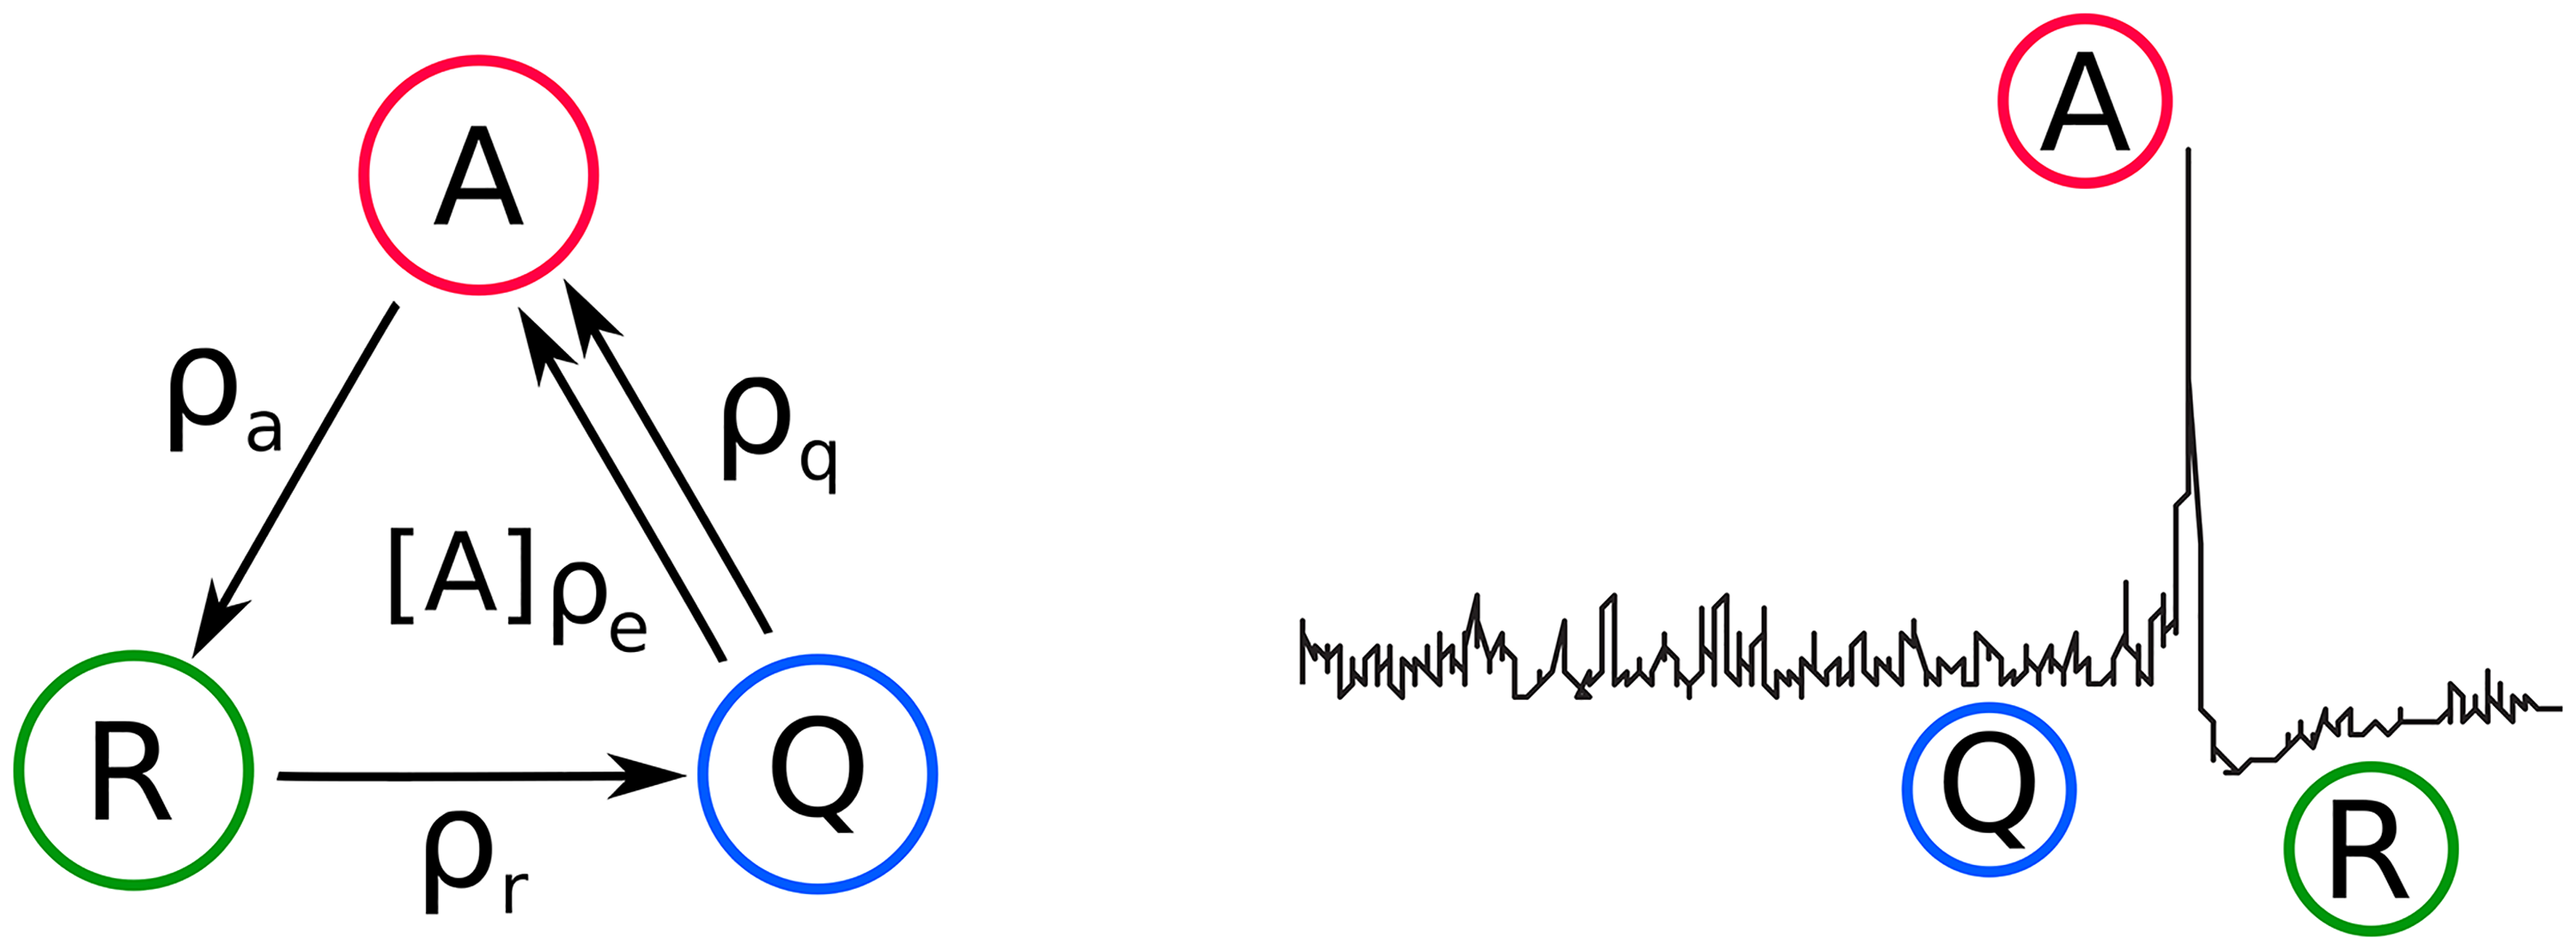
\includegraphics[width=\imsize]{estadoneuronas.png}
	\caption[Modelo neural de 3 estados quiescente-activo-refractario (QAR) .]{Modelo neural de 3 estados quiescente-activo-refractario (QAR). Las células en la retina en desarrollo se modelan con tres estados de actividad. Las células activas ( A ; rojo) disparan ráfagas de potenciales de acción, antes de volverse refractarias ( R ; verde) durante un período prolongado de tiempo. Las células inactivas ( Q ; azul) pueden estallar espontáneamente o pueden ser reclutadas en una ola por otras células activas.} 	\label{fig:estadoneuronas}
\end{figure}




\section{Discusión}
	
El presente capítulo se centró en la dinámica neuronal del cerebro de un organismo, destacando su naturaleza incesante y la exhibición constante de patrones espacio-temporales complejos de actividad coordinada, aun en la inactividad. Estas características de flexibilidad y adaptabilidad son fundamentales para enfrentar los desafíos ambientales relacionados con la supervivencia y la reproducción, y probablemente se originan debido a presiones evolutivas \cite{haimovici_dynamical_2016}. Se ha propuesto que estos patrones complejos emergen de la interacción entre la topología compleja del sistema nervioso del organismo y la dinámica de las neuronas individuales. En concreto, las redes neuronales en los cerebros de los organismos presentan características como longitudes de camino cortas, coeficientes de agrupamiento elevados y distribuciones de grado sesgadas. Estas arquitecturas altamente complejas influyen significativamente en los procesos que ocurren en las redes, lo que sugiere que el cableado neuronal puede ser crucial para la generación de oscilaciones y sincronización en el cerebro. Además de esta estructura altamente heterogénea y compacta, las redes neuronales también exhiben ruido intrínseco. Aunque las neuronas están sujetas a fluctuaciones térmicas que actúan como una fuente externa de ruido, la mayor parte de la variabilidad en los circuitos parece provenir de la actividad generada dentro de las propias redes neuronales. Esto implica que un enfoque estocástico es inevitable para abordar las actividades neuronales. A pesar de que inicialmente el ruido podría parecer perjudicial, en las redes neuronales puede tener un papel positivo al favorecer oscilaciones y sincronización, o al inducir resonancia estocástica.


El resultado más significativo de este capítulo es la formulación de un modelo de dinámica neuronal que exhibe todas las características mencionadas anteriormente. Este modelo integra una arquitectura de red basada en el conectoma del C. elegans, el cual posee propiedades topológicas complejas similares a las de un organismo real. Además, se incorpora una dinámica de red estocástica que representa el ruido intrínseco presente en las redes neuronales reales. Esta compleja interacción permite que la red exhiba estados de actividad irregular intrínsecamente generados, similares a la actividad coordinada que emerge del estado de reposo. La lógica computacional de este modelo se basa en la generación de eventos dinámicos locales y su comunicación global a través de la arquitectura de red característica. La generación de eventos se fundamenta en la acumulación de entradas en los nodos susceptibles, los cuales son excitados más allá de un umbral de entrada crítico. Después de su activación, los nodos pueden entrar en un período refractario durante el cual no pueden generar nuevos eventos, antes de regresar a un estado susceptible. Este ciclo básico de activación e inactividad es el sello distintivo de los medios excitables discutidos en el \cref{sec:mediosexcitables}. A pesar de su aparente simplicidad, este mecanismo básico puede dar lugar a dinámicas globales ricas cuando se combina con una organización de red heterogénea, como la proporcionada por el conectoma.

El modelo se implementa como un autómata celular estocástico, lo que lleva a la discusión de los autómatas celulares en este capítulo. Los autómatas celulares son sistemas dinámicos en grafos en los cuales los vértices tienen un conjunto finito de estados en tiempos discretos $t$. Los estados de los vértices cambian según una regla de actualización homogénea (la misma regla se aplica a todos los vértices) y local (la regla depende solo de una vecindad finita del vértice en cuestión). Aunque los autómatas celulares están definidos por reglas simples, pueden exhibir comportamientos dinámicos complejos a gran escala. De esta manera, ofrecen un mundo microscópico ficticio que reproduce la física correcta a una escala de granularidad gruesa, siendo la contrapartida del concepto físico de \textquote{campo}. Enfocándonos en las propiedades colectivas, es razonable buscar modelos mínimos que, incluso careciendo de reglas microscópicas realistas, puedan reproducir un comportamiento macroscópico relevante. Dadas las ventajas y características de los autómatas celulares, la dinámica de red del modelo se implementó en este marco matemático. Los autómatas celulares (AC) son una herramienta clave en la simulación de fenómenos naturales debido a su capacidad de proyectar y describir fenómenos simulados en un marco matemático adecuado. Además, describen una arquitectura masivamente paralela en la cual se puede implementar el simulador. El enfoque de los autómatas celulares es efectivo cuando la simplificación de las leyes microscópicas relacionadas con un fenómeno dado no es relevante a una escala macroscópica de observación. La mecánica estadística nos enseña que este hecho suele ser cierto para sistemas cuya complejidad surge de un comportamiento colectivo en lugar de aspectos distintivos de las interacciones microscópicas.


Por último, con el marco teórico presentado en este y los capítulos anteriores, estamos en condiciones de desarrollar los métodos y experimentos computacionales necesarios para confirmar o refutar la hipótesis de que la dinámica del cerebro de C. elegans inmovilizados opera cerca de un punto crítico. El siguiente capítulo presentará los resultados obtenidos al aplicar herramientas que permiten detectar firmas de criticidad tanto en experimentos con C. elegans reales como en la dinámica global que emerge del modelo. En el caso del modelo, realizaremos una caracterización cuantitativa de los regímenes dinámicos mediante el análisis estadístico del tamaño de los clústeres activos en el estado estacionario a lo largo del tiempo. Los clústeres se definen como conjuntos de nodos conectados que están activos simultáneamente, y su tamaño se calculará en cada paso de tiempo. Esta estrategia nos permitirá emplear las herramientas de la teoría de percolación que se presentaron en el \cref{sec:cap-percolacion}. En relación a los experimentos con gusanos inmovilizados, buscaremos propiedades de criticidad, como la presencia de cascadas espacio-temporales de actividad neuronal denominadas avalanchas neuronales.   La teoría de las transiciones de fase distingue diferentes tipos de dinámicas en los sistemas físicos. Se introducirán las herramientas estadísticas para detectar este tipo de fenómenos, y se discutirá cómo se aplicarán a los datos reales.   La detección de estas propiedades permitirá establecer un paralelismo entre el comportamiento de la dinámica cerebral del gusano real y las predicciones del modelo.

	
Concluyendo, Los anteriores capítulos sientan las bases teóricas necesarias para explorar la dinámica neuronal y su relación con la criticidad en el cerebro de C. elegans. El modelo de autómatas celulares se presenta como una herramienta valiosa para estudiar la aparición de patrones complejos de actividad coordinada en redes neuronales. La combinación de este modelo con herramientas de la teoría de percolación, la teoría crítica y la mecánica estadística nos permitirá identificar signos de criticidad, respaldando así la hipótesis de que el cerebro de C. elegans, incluso en estado inmovilizado, opera cerca de un punto crítico. Los resultados obtenidos en el siguiente capítulo serán esenciales para comprender mejor la dinámica cerebral y su relevancia en el procesamiento de información y la adaptabilidad en organismos más complejos.





















\chapter{Dinámica neuronal experimental del C. elegans}\label{cap:resultado_critico}
\graphicspath{{figs/capitulo_resultado_critico/}}

\chapterquote{dynamical systems with extended spatial
	degrees of freedom naturally evolve into self-organized critical structures of states which
	are barely stable. The combination of dynamical minimal stability and spatial scaling
	leads to a power law for temporal fluctuations}{Bak}

Este apartado presenta los resultados de los experimentos realizados con datos experimentales del nematodo C. elegans. El objetivo central de este análisis es examinar si el sistema nervioso de este organismo exhibe características de criticidad neuronal. Para lograrlo, se recopilaron datos de actividad neuronal en gusanos inmovilizados proporcionados por investigaciones previas y se aplicaron diversas métricas. Estos experimentos proporcionarán una comprensión más profunda acerca de si el C. elegans muestra propiedades típicas de la criticidad neuronal a nivel microscópico.

Este apartado se centra en la exposición de los datos experimentales recopilados, los métodos empleados en su análisis y, en última instancia, los resultados obtenidos. Exploraremos en detalle las métricas de criticidad aplicadas y cómo estas han revelado patrones y propiedades específicas en la actividad neuronal. También examinaremos las implicaciones de estos resultados en el contexto de nuestra hipótesis principal y su posible relevancia en los campos de la neurociencia y la investigación computacional.

A lo largo de este apartado, se evaluará la coherencia de los hallazgos con la teoría de la criticidad neuronal y cómo estos resultados contribuyen a una comprensión más completa de la dinámica neuronal en el C. elegans. Además, se considerarán las posibles limitaciones y alcances de estos resultados experimentales.


%Las cuatro características que acabamos de describir se observan comúnmente en sistemas complejos que experimentan una transición de fase orden-desorden [1, 10, 13]. Este escenario fue explorado en [58] definiendo un parámetro de control y un parámetro de orden a partir de los datos
%
%Para representar el grado de orden (es decir, el parámetro de orden), se calculó el tamaño del grupo más grande (normalizado por el número de sitios activos) en todo el cerebro y se representó en función del número de puntos activos (es decir, el parámetro de control). Esto se hizo para todos los pasos de tiempo y se representó en la Figura 3.7e (círculos pequeños). Como parámetro de control, se utilizó el nivel global de actividad como en otros modelos bien estudiados de transiciones orden-desorden (el ejemplo más claro es la percolación [59]).
%
%
%El mismo razonamiento lleva a la conjetura [1, 6, 7] de que la complejidad de la dinámica cerebral es solo otra firma de un proceso crítico subyacente. Debido a que el mayor número de estados metaestables existe en el punto cercano a la transición, el cerebro puede acceder al mayor repertorio de comportamientos de manera flexible. Esa visión afirmó que las propiedades más fundamentales del cerebro solo son posibles manteniéndose cerca de esa inestabilidad crítica, independientemente de cómo se alcance o mantenga dicho estado. En las siguientes secciones, se analiza la evidencia empírica reciente que apoya esta hipótesis.
%La presencia de escalado y correlaciones que abarcan el tamaño del sistema suelen ser indicios de fenómenos críticos. Si bien, en principio, es relativamente sencillo identificar estas firmas, en el caso de datos finitos y la ausencia de una teoría formal, como es el caso del cerebro, cualquier indicio inicial de criticidad debe verificarse con muchos artefactos conocidos. En los próximos párrafos, discutimos los esfuerzos más relevantes para identificar estas firmas en datos cerebrales a gran escala.
%
%a aplicación de este nuevo método permitió, por primera vez, definir un marco teórico en términos de un parámetro de orden y control derivado de los datos de fMRI, donde el régimen dinámico puede interpretarse como uno correspondiente a un sistema cercano al punto crítico de una transición de fase de segundo orden. El análisis demostró que el cerebro en reposo pasa la mayor parte del tiempo cerca del punto crítico de dicha transición y exhibe avalanchas de actividad regidas por las mismas propiedades dinámicas y estadísticas descritas anteriormente para los eventos neuronales a escalas más pequeñas.
%
%Esto se explora aquí compilando las estadísticas y la dinámica de los grupos de puntos tanto en el espacio como en el tiempo. Los grupos son grupos de vóxeles contiguos con señales por encima del umbral en un momento dado, identificados por un algoritmo de escaneo en cada volumen de fMRI. La Figura 3.7a muestra ejemplos de grupos (en este caso no consecutivos en el tiempo) representados con diferentes colores. Por lo general (Figura 3.7b, arriba), el número de grupos en un momento dado solo varía un orden de magnitud alrededor de la media (50). Por el contrario, el tamaño del grupo activo más grande fluctúa ampliamente, abarcando más de cuatro órdenes de magnitud.


%\chapterquote{...Why should it take an infinite amount of logic to figure out what a tiny piece of space/time is going to do? So I have often made the hypothesis that ultimately physics will not require a mathematical  statement, that in the end the machinery will be revealed, and the laws will turn out to be simple, like the chequer board with all its apparent complexities }{Richard P. Feynman}

%
%Los resultados presentados en esta Carta muestran que se pueden predecir aspectos muy relevantes de la dinámica cerebral a partir de la estructura, siempre que la dinámica subyacente sea crítica. Para guiar nuestra comparación con los resultados experimentales disponibles, elegimos concentrarnos en hallazgos sólidos sobre la dinámica cerebral. Específicamente, preguntamos cómo la dinámica cerebral espontánea a gran escala se organiza en los relativamente pocos patrones espaciotemporales revelados experimentalmente en los últimos años [4]. Esto es importante porque una amplia gama de experimentos que utilizan imágenes de resonancia magnética funcional (fMRI) ha enfatizado que estos grupos espaciales de actividad coherente, denominados redes de estado de reposo (RSN) [5], están específicamente asociados con sistemas neuronales responsables de sensorial, cognitiva, y funciones conductuales
%
%
%El cerebro animal está compuesto por miles de millones de neuronas, que interactúan entre sí a través de miles de sinapsis por neurona. El resultado de tal interacción es la aparición de patrones espaciotemporales complejos de actividad neuronal que respaldan la percepción, la acción y el comportamiento. Una propuesta reciente considera al cerebro como una red de neuronas preparadas cerca de una transición dinámica [1–4], un punto de vista que está respaldado por resultados experimentales obtenidos de animales tanto in vitro [5] como in vivo [6], así como de estudios completos. experimentos humanos de neuroimagen cerebral [7-9].
%
%
%
%% Homeostatic plasticity and emergence of functional networks in a whole-brain model at criticality
%Estas ideas han sido particularmente investigadas en los últimos quince años en neurociencia y la hipótesis de que el cerebro está cerca de un estado crítico (en mecánica estadística sensu) está ganando consenso en la comunidad neurocientífica14,17,23–25. En los sistemas cerebrales, el concepto de criticidad está respaldado principalmente por los siguientes dos hallazgos experimentales: (i) el descubrimiento de avalanchas neuronales libres de escala19, como se describe mediante distribuciones de ley de potencia para el tamaño y la duración de los estallidos espontáneos de actividad en la corteza; (ii) la presencia de correlaciones temporales de largo alcance en las fluctuaciones de amplitud de las oscilaciones neuronales26,27. Otros estudios informaron sobre la universalidad de los exponentes de la ley de potencia encontrados originalmente en 19 entre diferentes especies, por ejemplo, rata28; primates no humanos29,30 y humanos mediante diversas técnicas, como MEG31–33; EEG34 y fMRI15,35. También desde un punto de vista teórico, muchos modelos de cerebro completo describen al máximo las actividades neuronales reales cuando se encuentran en un punto crítico15,19,35–38.
%
%
%
% La hipótesis emergente es que los sistemas vivos, o partes de ellos, como el cerebro, se acercan espontáneamente a una transición de fase crítica (estrictamente hablando, las transiciones de fase existen solo para sistemas con un número infinito de grados de libertad, que en el mejor de los casos son una buena aproximación de sistemas grandes, pero finitos, como un cerebro)16,17, lo que les confiere las características emergentes de los sistemas críticos como la falta de escalas espaciales y temporales y la alta capacidad de respuesta a las perturbaciones externas. Estas características se traducirían en la capacidad del cerebro, a través de una actividad de gran escala espacial y temporal, para reaccionar rápidamente ante estímulos externos generando un comportamiento global coordinado18, para maximizar la transmisión de información19,20, la sensibilidad a los estímulos sensoriales 21 y el almacenamiento de información22.
%
%
%
%
%Desde un punto de vista teórico, la física estadística ha contribuido decisivamente a resaltar la ventaja potencial que puede tener un cerebro en un estado crítico y también proporciona una descripción cuantitativa de las actividades cerebrales a través de modelos mesoscópicos minimalistas14,15. Los sistemas que constan de muchos componentes microscópicos (p. ej., neuronas) pueden exhibir tipos bastante diversos de comportamiento colectivo macroscópico con diferentes niveles de organización interna (p. ej., actividad cerebral). Además, ligeros cambios en los estímulos externos (p. ej., auditivos, visuales, etc.) o en la fuerza de las propias interacciones pueden inducir cambios estructurales drásticos, es decir, transiciones de fase. Por lo tanto, es tentador plantear la hipótesis de que los estados biológicos podrían ser manifestaciones de fases colectivas similares y que los cambios entre ellos podrían corresponder a transiciones de fase.
%
%
%
%La hipótesis del cerebro crítico establece que las redes neuronales biológicas, debido a su arquitectura estructural y funcional, trabajan cerca de las transiciones de fase para una respuesta óptima a las entradas internas y externas. Por lo tanto, la criticidad proporciona funciones y capacidades de comportamiento óptimas. Este capitulo pureba  esta hipótesis en la dinamica neuronal de C. elegans reales examinando la influencia de la lesión cerebral (ictus) en la criticidad de la dinámica neuronal estimada a nivel de sujetos individuales utilizando modelos de cerebro completo.
%
%
%Recientemente se ha encontrado evidencia de dinámica crítica tanto en experimentos como en modelos de dinámica cerebral a gran escala.
%
%Encontramos que la variación de los parámetros topológicos puede dar lugar a un comportamiento invariante de escala que pertenece a la clase de universalidad de percolación de campo medio o que tiene exponentes críticos no universales.
%
%El estudio de la actividad funcional cerebral ha revelado la existencia de fluctuaciones correlacionadas e invariancia de escala similares a las observadas en los fenómenos críticos. Tal evidencia provocó la conjetura de que la organización a gran escala del cerebro emerge en la criticidad [1-3].
%
%
%
%
%
%El documento está organizado de la siguiente manera. en la seg. II se describe el modelo, así como los métodos de simulación y escalado de tamaño finito utilizados. Los resultados se presentan en la Sec. tercero Discutimos la relevancia de los principales hallazgos en la Sec. IV.
%


%\section{Introducción}



%Traducción al español:
%
%En estas notas, discutimos la idea propuesta hace dos décadas por Bak [1] de que el cerebro en funcionamiento se mantiene en un régimen intermedio (crítico) caracterizado por correlaciones de ley de potencia. Una dinámica cerebral altamente correlacionada produce estados sincronizados sin valor conductual, mientras que una dinámica débilmente correlacionada impide el flujo de información. Entre estos estados, las características dinámicas únicas del estado crítico dotan al cerebro de propiedades que son fundamentales para el comportamiento adaptativo. Esta simple propuesta está ahora respaldada por un amplio conjunto de pruebas empíricas a diferentes escalas, que demuestran que la dinámica espaciotemporal del cerebro exhibe las firmas clave de la dinámica crítica, previamente reconocidas en otros sistemas complejos.
%
%
%Los circuitos neuronales muestran complejos patrones de actividad temporal espontáneos y evocados por estímulos. Como los transitorios de calcio dentro de las neuronas individuales reflejan uno o más eventos de potenciales de acción, la coincidencia temporal de los transitorios de calcio entre las neuronas ofrece una oportunidad para caracterizar la estructura de la red.  Una característica destacada de los sistemas dinámicos interconectados es su capacidad para sincronizarse (Acebrón et al., 2005). In vivo, la sincronización desempeña un papel más general al unir grupos de ensamblajes neuronales distribuidos en unidades funcionales para que estos ensamblajes puedan transferir información más fácilmente (Melloni et al., 2007; Uhlhaas et al., 2008; Uhlhaas y Singer, 2006; Womelsdorf et al., 2007). Para identificar grupos de neuronas con un patrón de actividad similar y cuantificar su sincronía	

%
%Realizamos simulaciones para varios valores del parámetro de control T que los resultados previos [16] indican que produce dinámicas subcríticas (para valores muy altos de T), supercríticas (para valores muy bajos de T) o críticas. Para acumular suficientes estadísticas, ejecutamos 20 simulaciones numéricas (que duran 105 pasos de tiempo, descartando los 5000 pasos de tiempo iniciales). Para cada simulación construimos una red con los mismos parámetros promedio  k y pi  (es decir, son realizaciones estocásticas). Para imitar situaciones experimentalmente relevantes, registramos la dinámica de las neuronas dentro de una ventana cuadrada de neuronas W × W (con W <= L), vea la Fig. 1-a.
%
%Si el sistema presenta un punto crítico similar a la percolación, se espera que tanto s como S 2 exhiban un máximo (dependiente del tamaño) para un cierto valor pseudocrítico del parámetro de control (el umbral T en el presente caso)
%
%
%Para caracterizar la transición entre estos regímenes se definió un parámetro de orden considerando los tamaños de los clusters activos. Los clústeres son grupos de nodos activados simultáneamente y vinculados entre sí a través de un w distinto de cero. En cada paso de tiempo se calcularon los tamaños del grupo más grande (S1) y el segundo grupo más grande (S2). 
%
%
%n un valor intermedio, un punto crítico [Tc en el panel (c) de la Fig. 1] puede identificarse por el pico en el tamaño del segundo grupo más grande, como se hace generalmente en percolación [16], así como recientemente en IRMf humana experimentos [10]. El tamaño finito del conectoma disponible hace que la demostración habitual de criticidad en el límite termodinámico no sea práctica; por lo tanto, en su lugar, se proporciona una gama de indicadores alternativos (ver también el Material Suplementario [17])
%
%Como ya se mencionó, la distribución de tamaños de conglomerados de actividad puede ser informativa de los diferentes regímenes dinámicos del modelo. Calculamos tales medidas como una función del umbral T
%
%
%
%Como se discutió en el \cref{cap:dinamica_critica} los mecanismos fundamentales que subyacen a la dinámica de la actividad cerebral aún se desconocen en gran medida. La investigación neurocientífica interdisciplinaria, inspirada en la física estadística, ha sugerido que la dinámica neuronal del cerebro de los organismos permanece cerca de un estado crítico, es decir, en la vecindad de una fase crítica de transición entre orden y desorden, o entre actividad oscilatoria asincrónica o sincrónica.  De  hecho, los sistemas neuronales parecen mostrar características  de los sistemas en estado crítico. Estos incluyen i) la invariancia de escala de las avalanchas neurales  reportadas en diversas especies, por ejemplo, ratas \cite{gireesh_neuronal_2008}, primates no humanos \cite{petermann_spontaneous_2009, yu_higher-order_2011}, imágenes de calcio de cerebro completo de pez cebra \cite{ponce-alvarez_whole-brain_2018}  y humanos a través de diferentes técnicas de imagen y señales electrofisiológicas; ii) la presencia de correlaciones espacio-temporales de largo alcance en las fluctuaciones de amplitud de las oscilaciones neuronales, incluida la observación de espectros de potencia $1/ f$ de señales MEG/EEG registradas simultáneamente.  iii)   la distribución del tamaño de los clústeres  en señales BOLD de la conectividad estructural del cerebro humano  \cite{haimovici_brain_2013}. 
%
%Por otra parte  desde mediados de la década de los 90, la intrigante dinámica del cerebro en reposo ha atraído un creciente cuerpo de investigación en neurociencia. Los estudios de neuroimagen han revelado distintas redes funcionales que se activan y desactivan lentamente, lo que apunta a la existencia de una dinámica de red subyacente que emerge espontáneamente durante el reposo, con características espaciales, temporales y espectrales específicas. Si bien la actividad en reposo  se mide comúnmente en humanos, ha sido menos común hacerlo en modelos animales debido a limitaciones técnicas. Sin embargo, se han aplicado técnicas de imagen  en animales, pero generalmente requieren anestesia o fijación de la cabeza. Más recientemente, los avances en la obtención de imágenes de sensores de voltaje o calcio in vivo han sido reconocidos como otro enfoque para evaluar la conectividad funcional en modelos animales despiertos. Se han logrado avances significativos con estas técnicas, que ahora pueden generar imágenes de miles de neuronas y grandes volúmenes de corteza en roedores que se comportan libremente. Si bien estos avances permiten nuevas y emocionantes formas de estudiar la dinámica de la población neuronal in vivo, estos enfoques aún no permiten obtener imágenes de todo el cerebro.
%
%Dada la importancia de   estudiar la criticidad en el sistema nervioso, es deseable monitorear la dinámica de todo el cerebro con  resolución de una sola célula.  En este capitulo  utilizando   los datos de la  la actividad cerebral de  imágenes de calcio en todo el cerebro de  C. elegans  inmovilizados en un dispositivo microfluídico  de experimentos realizados por  Kato et al \cite{kato_global_2015}, Kaplan et al \cite{kaplan_nested_2020}  y mas recientemente Yeminiet al \cite{yemini_neuropal_2021} se buscara aportar a  los pocos estudios existentes sobre la criticidad neuronal en un sistema  a nivel de de todo el cerebro.  Queremos resolver la pregunta de que si en un organismo con un sistema nervioso tan reducido como el C. elegans  ($\sim 302$ )  existen evidencias de criticidad neuronal.  Abordamos  esta pregunta abierta estudiando las estadísticas de la dinámica del cerebro completo del  C.  elegans e interpretándolas en el marco de la criticidad. Específicamente, utilizamos los datos de los experimentos   para monitorear la dinámica de todo el cerebro con una resolución de  una sola neurona. Con este enfoque, podremos estudiar la dinámica colectiva de la actividad neuronal y su propagación por todo el cerebro, en forma de avalanchas  y  clústeres neuronales. 
%
%Nuestra  hipótesis es que estos fenómenos críticos surgen de la interacción entre la estructura cerebral a gran escala y la dinámica neuronal a nivel local. Para abordar  la pregunta de que si la dinámica neuronal del C. elegans tiene evidencias de ser critica  adoptamos  un enfoque de modelado híbrido que combina el conectoma del C. elegans hermafrodita  con  registros   de   series temporales de la dinámica neuronal  de los tres experimentos   con C. elgans  anteriormente descritos.   De esta combinación se desea encontrar  una serie de resultados consistentes con los estudios existentes de criticidad neuronal. Se estudiaron  dos firmas  de  criticidad en los datos: la invariancia de escala en avalanchas neuronales \cite{plenz_critical_2013} y la distribución de clústeres de neuronas sincronizadas \cite{haimovici_brain_2013} . Es importante analizar los patrones de actividad espaciotemporal  porque los comportamientos invariantes de escala observados en la criticidad no dependen de los detalles microscópicos del sistema. En cambio, a menudo dependen de la dimensión del sistema y del tipo de transición de fase. Por lo tanto, un sistema en estado crítico tiene propiedades universales que pueden explicarse mediante modelos matemáticos simples los cuales serán explorados en la siguiente sección.


\section{Dinamica neuronal experimentos C. elegans}\label{sec:umbralizacion}

 Para estudiar los patrones de actividad espaciotemporal que emergen de la dinámica de todo el cerebro, analizamos la actividad neuronal de 5 gusanos hermafroditas inmovilizados  de experimentos realizados por Kato et al \cite{kato_global_2015},   5 gusanos hermafroditas de experimentos realizados por Kaplan et al \cite{kaplan_nested_2020} y 21 gusanos hermafroditas de experimentos realizados por Yeminiet et al \cite{yemini_neuropal_2021}, cuyo  conjunto de datos se pueden encontrar en los repositorios OSF \cite{Zimmer_2022,Zimmer_20222} y  Zenodo \cite{eviatar_yemini_2020_3906530} respectivamente.  Como se discutió en el capitulo C. elegans,   en los experimentos de Kato et al y Kaplan et al  en cada animal se registraron la actividad cerebral en condiciones ambientales constantes durante \qty{18}{\minute } y \qty{30}{\minute}  respectivamente. La actividad de todo el cerebro se caracterizó por la activación de grupos de neuronas  que podían abarcar grandes partes del cerebro. Nuestro objetivo fue describir las estadísticas de estos eventos.  Para la extracción de fluorescencia y la inferencia de spikes utilizamos los métodos descritos en el \cref{sec:inferencia_spikes}.  Los parámetros utilizados para cada uno de estos enfoques  se encuentran de manera automática.  
 
 
 En esta sección, probamos el rendimiento de los algoritmos en los datos reales. Por simplicidad solo se mostraran los resultados del conjunto de datos RIShisCl  del gusano 1 de los experimentos de Kaplan \cite{Zimmer_20222}. Cabe resaltar que en el resto de experimentos se obtuvieron  resultados similares.  Para implementar el algoritmo de deconvolución  OASIS utilizamos la biblioteca de código abierto CaImAn \cite{giovannucci_caiman_2019}, el algoritmo MCMC esta implementado en MATLAB cuyo código esta disponible en \url{https://github.com/epnev/continuous_time_ca_sampler}, para el procedimiento de búsqueda de picos de Kaplan et al. se utilizo un algoritmo de python a medida.   Finalmente CASCADE no necesita  ninguna instalación, ya que todo el algoritmo se ejecuta en la nube en un cuaderno de Google Colab \url{https://github.com/HelmchenLabSoftware/Cascade}.    Aunque los métodos basados en modelos son, en principio, no supervisados, es necesario ajustar varios parámetros para lograr el máximo rendimiento, por tanto todas las implementaciones tienen autoajustes que encuentran el valor mas optimo de los parámetros en los datos.
 
 \subsection{OASIS}
 
 Para realizar la deconvolución utilizamos la función de CaImAn  \textbf{constrained\_foopsi}\footnote{\url{https://caiman.readthedocs.io/en/master/core_functions.html}}   cuyo resultado es inferir el tren de spikes discretizado más probable subyacente a una traza de fluorescencia. Para la intensidad de fluorescencia $y$ (ver \Cref{eq:86}) se utilizo   la traza $\Delta F/F$ corregida de  bleaching .  Dado que los datos se registran a una frecuencia de  \qty{3.0303}{\Hz}, la serie neuronal resultante consta de 5455 puntos temporales para un total de \qty{30}{\minute}.   Centramos nuestro análisis en  la neurona AVAL.  Esta neurona fue elegida debido a su importante rol biológico   como también su gran grado de conectividad. Es importante resaltar que en las otras series neuronales del conjunto de datos se obtuvieron resultados similares.     Para mejorar  la precision de la inferencia  utilizamos la restricción sobre el tamaño mínimo de los spikes, con esta opción el algoritmo varia un umbral hasta que el RSS cruza el umbral $\sigma^2T$.    La adición de esta restricción ayuda a  tomar una decisión binaria sobre si asignar un spike o no en un determinado tiempo $t$.    Finalmente  la función también estima los parámetros    del modelo a partir de los datos.
 
 Los resultados se muestran en las \Cref{f:oasis_p1,f:oasis_p2}.  La traza de fluorescencia observado se muestra con una línea rosada y un marcador en forma de estrella en ambas figuras.   Si $p = 1$ (\Cref{f:oasis_p1}), entonces el transitorio de calcio en respuesta a un spike se modela por una función exponencial que aumenta instantáneamente y se desintegra lentamente.  Esto se recomienda cuando la constante de tiempo de subida es pequeña en comparación con la longitud del intervalo de tiempo.   El marco AR(1) propuesto hace una serie de suposiciones simplificadoras sobre la dinámica de fluorescencia, con el beneficio de una mayor trazabilidad computacional. Se supone que la dinámica es lineal e invariante en el tiempo, y no se asume ningún nivel de saturación. Es posible encontrar claras violaciones de estos supuestos en la \Cref{f:oasis_p1}: en $t\approx1125$ el algoritmo infiere unos spikes de pequeña amplitud que no estarían presentes en la traza neuronal.     Si queremos modelar explícitamente el tiempo de subida, elegimos $p = 2$ (\Cref{f:oasis_p2}). El método AR(2) mejora notablemente el  resultado de la deconvolución, adaptándose mejor a la dinámica neuronal.  Como se ve en la \Cref{f:oasis_p2} este método reduce eficazmente el ruido de la traza de fluorescencia observada y es  capas   de  deconvolver la actividad de los spikes correctamente. 
 
 
 
 
   \begin{figure}[h!]
 	\centering{}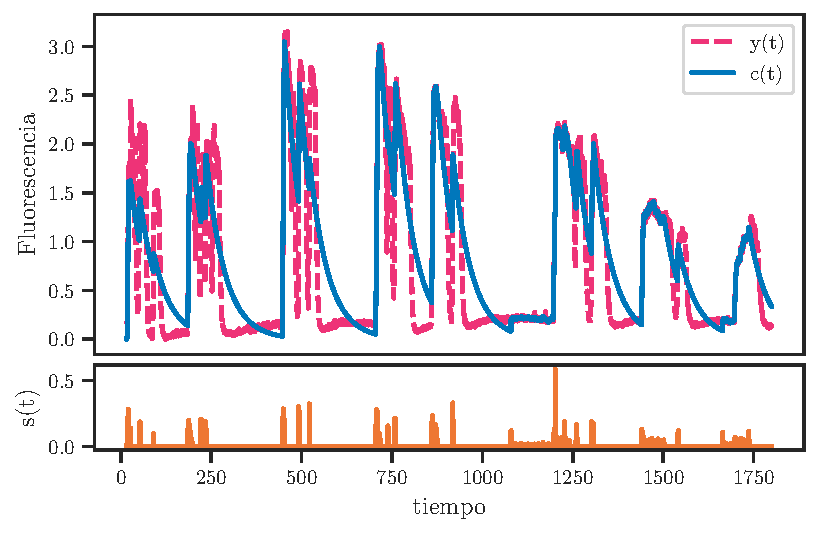
\includegraphics[width=\imsize]{oasis_p1.pdf}
 	\caption[Modelo autorregresivo generativo para la dinámica del calcio de la neurona AVAL.]{Modelo autorregresivo generativo para la dinámica del calcio de la neurona AVAL. El tren de spikes $s(t)$ se filtra para producir la traza de calcio $c(t)$; se utilizó $p = 1$ como orden del proceso AR. El ruido añadido por las mediciones produce la fluorescencia observada $y(t)$. }\label{f:oasis_p1}  
 \end{figure}
 
    \begin{figure}[h!]
 	\centering{}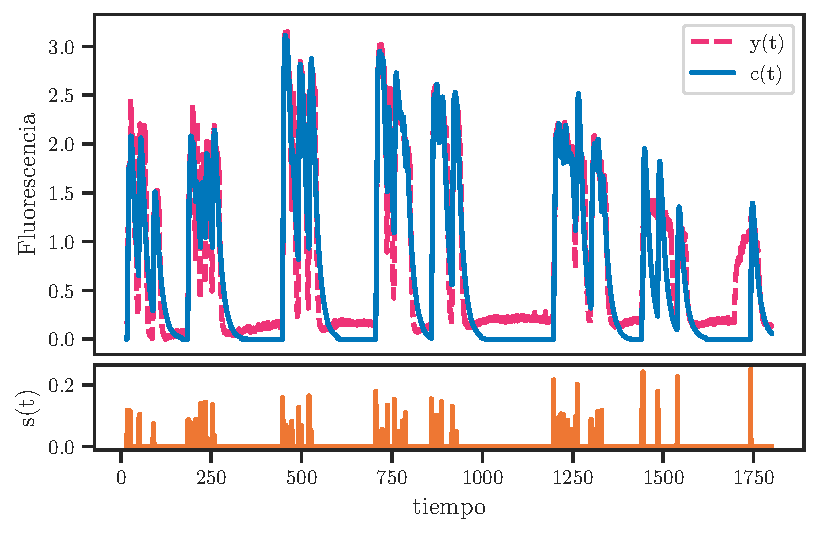
\includegraphics[width=\imsize]{oasis_p2.pdf}
 	\caption[Modelo autorregresivo generativo para la dinámica del calcio de la neurona AVAL.]{Modelo autorregresivo generativo para la dinámica del calcio de la neurona AVAL. El tren de spikes $s(t)$ se filtra para producir la traza de calcio $c(t)$; se utilizó $p = 2$ como orden del proceso AR. El ruido añadido por las mediciones produce la fluorescencia observada $y(t)$. }\label{f:oasis_p2}  
 \end{figure}
   
 Finalmente el marco AR tiene ciertas ventajas con respecto de los otros algoritmos estudiados en este apartado, como lo es el  permitir  un marco de modelado flexible e interpretable que conserva la trazabilidad computacional.   Además, los coeficientes AR se pueden estimar directamente a partir de los datos brutos de una manera completamente no supervisada, no requieren la existencia de spikes aislados para el ajuste fino de los distintos parámetros, y se pueden ajustar aún más durante el algoritmo de deconvolución \cite{pnevmatikakis_simultaneous_2016}. Aunque este marco AR(p) hace ciertas suposiciones simplificadoras sobre la linealidad y la dinámica del indicador de calcio, no obstante, da como resultado un estimador altamente eficiente desde el punto de vista computacional que alcanza un rendimiento de vanguardia entre los métodos no supervisados, como se ha demostrado  en Theis et al \cite{theis_benchmarking_2016}.
 
 \subsection{MCMC}
 
 Aunque el proceso de identificación de los parámetros AR del algoritmo OASIS suele ser muy útil para estimar la respuesta transitoria que surgiría de un solo spike, es útil refinar estas estimaciones dadas las estimaciones iniciales de los tiempos de spike. Para ello utilizamos  una extensión de los métodos Markov Chain Monte Carlo (MCMC) descritos en el \cref{sec:MCMC}. 
 
La \Cref{f:MCMC}(a) muestra la traza de calcio media obtenida con 500 muestras del algoritmo MCMC (azul) superpuesta a los datos reales (rosado), el método sigue  bastante bien la  traza de fluorescencia observada; el método MCMC puede modificar las constantes de tiempo inferidas para ajustarse mejor a los datos. Nótese que aquí el método MCMC se inicializó con los resultados obtenidos con el enfoque AR(2) explicado anteriormente. El método MCMC produce muestras de trenes de spikes con una resolución temporal continua y, por lo tanto, puede proporcionar más información sobre el número de spikes producidas en cada intervalo de tiempo y la incertidumbre de estas estimaciones debido al ruido y a la tasa de imagen finita. Esto se muestra en la \Cref{f:mcmc}, donde se traza la posterior marginal del número de spikes en cada intervalo de tiempo. Esta cuantificación de la incertidumbre temporal no está disponible con el algoritmo OASIS, que se basa en un marco de optimización convexa y, por lo tanto, proporciona una única estimación de la actividad neuronal, dividida en intervalos según la resolución de la tasa de imágenes.  El algoritmo predice la mayoría de los spikes ( \Cref{f:MCMC}c ) y proporciona estimaciones de baja varianza de los parámetros del modelo. Finalmente al comparar los metodos de deconvolución   AR(2)-MCMC (\Cref{f:MCMC}) obtiene mejores resultados que AR(2)-OASIS (\Cref{f:oasis_p2}). Ambos métodos superan al metodo  AR(1) (\cref{f:oasis_p1}), estableciendo que modelar el tiempo de subida puede mejorar significativamente la calidad de la deconvolución
 
 
 

    \begin{figure}[h!]
	\centering{}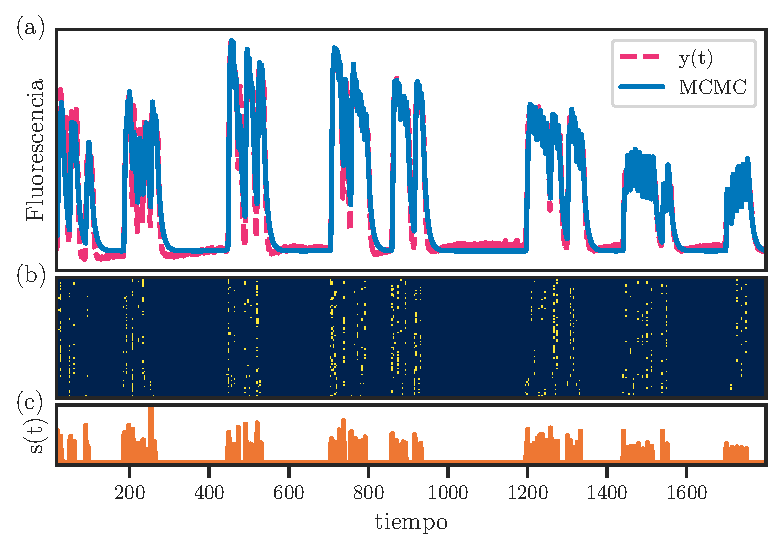
\includegraphics[width=\imsize]{MCMC.pdf}
	\caption[Aplicación del método MCMC.]{Aplicación del método MCMC. (a)  Datos de fluorescencia  de la neurona AVAL  y traza de fluorescencia reconstruida con  la  media de las muestras obtenida por el método MCMC completamente bayesiano con actualización de la constante temporal. El método MCMC  afina las constantes de tiempo para que se ajusten mejor a los datos observados.  (b)  Raster plot de los spikes de los  eventos del método MCMC. (c)  Actividad neuronal estimada  a partir de la media del marginal posterior por timebin con el método MCMC.  El método detecta con precisión los intervalos de bursting de las neuronas.  El método MCMC aunque más caro da una mejora significativa en la deconvolución de spikes comparado con el método OASIS. }\label{f:MCMC}  
\end{figure}


    \begin{figure}[h!]
	\centering{}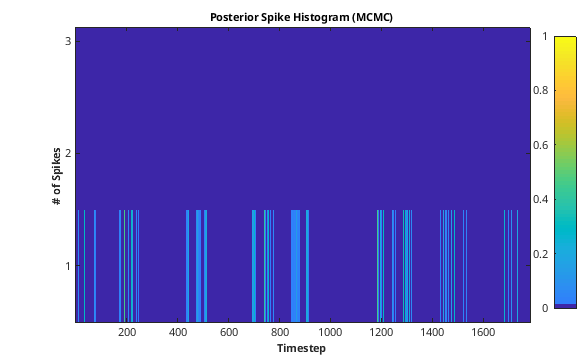
\includegraphics[width=\imsize]{mcmc.png}
	\caption[Aplicación del método MCMC.]{Representación codificada por colores del histograma marginal posterior empírico obtenido con el método MCMC. El mapa de colores muestra la probabilidad de un cierto número de spikes dentro de un timebin dado. El método MCMC puede cuantificar la incertidumbre e identificar múltiples spikes dentro de un mismo intervalo de tiempo.}\label{f:mcmc}  
\end{figure}

  
\subsection{Método de Kaplan  para detectar picos neuronales}

Aplicar diferencias finitas convencionales en los datos experimentales amplificará en gran medida cualquier ruido presente. La eliminación del ruido antes o después de la diferenciación no suele dar resultados satisfactorios. Un método que da buenos resultados es regularizar el propio proceso de diferenciación. Esto garantiza que la derivada calculada tendrá cierto grado de regularidad, hasta un punto que a menudo se puede controlar ajustando los parámetros. El marco que adoptaremos se encuentra en el \cref{C:ap1}. Sin embargo, el nivel y el tipo de regularización suelen imponerse de forma ad hoc, por lo que actualmente no existe un \textquote{mejor método} consensuado para obtener las derivadas \textquote{mejor ajustadas}. Para solventar este problema utilizamos un marco de optimización multiobjetivo para elegir los parámetros que equilibra dos métricas independientes.  Este enfoque minimiza una función de pérdida consistente en una suma ponderada de dos métricas calculadas a partir de la estimación de la derivada: la fidelidad de la integral de la derivada y su suavidad (\Cref{eq:ap:1}). Van breugel et al \cite{van_breugel_numerical_2020} sugieren estas métricas como aproximaciones para minimizar el error y el sesgo de la derivada estimada, y mostraron  que el barrido a través de los valores de un único hiperparámetro $\gamma$ produce estimaciones de la derivada que generalmente trazan el frente de Pareto de soluciones que minimizan el error y el sesgo. Es importante destacar que este marco de optimización no asume ningún conocimiento de la verdadera derivada subyacente y reduce la tarea de seleccionar muchos parámetros de cualquier algoritmo de diferenciación a la resolución de una función de pérdida con un único hiperparámetro. 

Para determinar un valor de $\gamma$  adecuada se utilizara  una heurística sencilla que es explicada en \cite{van_breugel_numerical_2020}  que se deriva del espectro de potencia y la resolución temporal de los datos. Todo este procedimiento se implementara  con el conjunto de herramientas Python de código abierto, pynumdiff.  Descubrimos que la mejor elección de $\gamma$ depende del contenido frecuencial de los datos.   En primer lugar, examinamos los espectros de potencia de los datos para elegir una frecuencia de corte que corresponda al inicio de la caída de potencia.  La \Cref{f:espectro_potencias_experimentos} muestra los espectros de potencia de los datos, indicando la frecuencia de corte (rojo) utilizada para seleccionar $\gamma$.  En cada conjunto de datos  la magnitud del ruido no cambia, esto se ve evidenciado  en que en un mismo experimento tanto los  espectro de potencias y la frecuencia de corte de las series neuronales son similares.  Esta frecuencia de corte, junto con la resolución temporal de los datos, se utilizan como entradas de la  heurística descrita por la \Cref{eq:84} para determinar un valor óptimo de $\gamma$.  

\begin{figure}[h!]
	\centering{}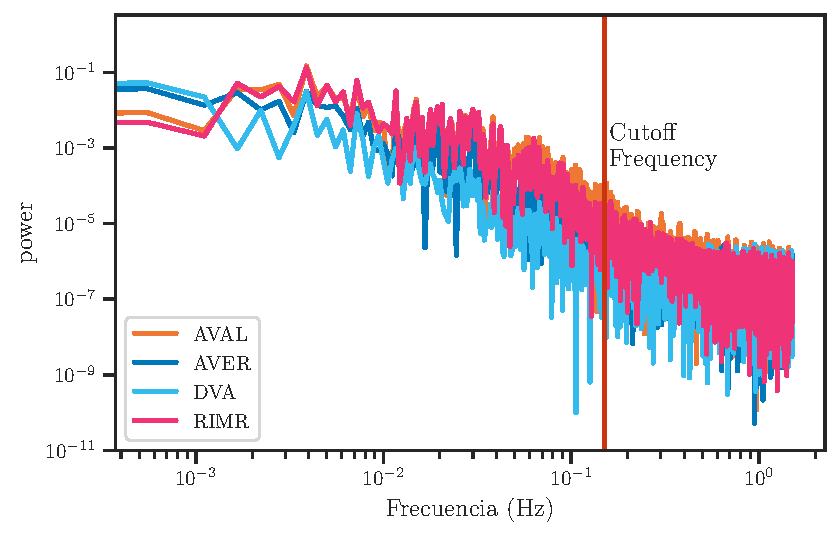
\includegraphics[width=\imsize]{espectro_potencias_experimentos.pdf}
	\caption[La frecuencia de los datos se evalúa inspeccionando los espectros de potencia; la línea roja indica la frecuencia utilizada para determinar $\gamma$]{La frecuencia de los datos se evalúa inspeccionando los espectros de potencia algunas neuronas de las series neuronales correspondientes a  los experimentos  Kaplan; la línea roja indica la frecuencia utilizada para determinar $\gamma$. }\label{f:espectro_potencias_experimentos}  
\end{figure}

Con $\gamma$ elegido, minimizamos nuestra función de pérdida de la \Cref{eq:ap:1} para encontrar los parámetros óptimos para la diferenciación numérica. La \Cref{f:resultado_picos}(naranja)   muestra  la derivada   de la serie temporal de la neurona AVAL de uno de los cinco gusanos de los experimentos de Kaplan \cite{kaplan_nested_2020}.   Habiendo encontrado  la derivada para inferir los spikes discretos utilizamos el método descrito en el \Cref{sec:metodos_picos}.   Este método depende de dos parámetros. En primer lugar, todos los métodos de detección de picos dependen en gran medida del grado de suavizado de los datos, que se logra en nuestro caso ajustando el hiperparámetro $\gamma$. En segundo lugar, la gama de deltas probados determina si este método tendrá éxito o no. Si el intervalo de deltas está dominado por deltas demasiado bajos o demasiado altos, no encontrará un punto de cambio adecuado, o el punto de cambio será demasiado liberal o demasiado conservador para todas las trazas. En este trabajo para determinar el rango delta  para una traza particular se utilizó la desviación estándar, estableciendo este valor como el máximo del rango delta, mientras que el mínimo y el intervalo entre deltas se establecían como la desviación estándar dividida por 100. La   \Cref{f:resultado_picos}(rosada) muestra los spikes inferidos por este método.




\begin{figure}[h!]
	\centering{}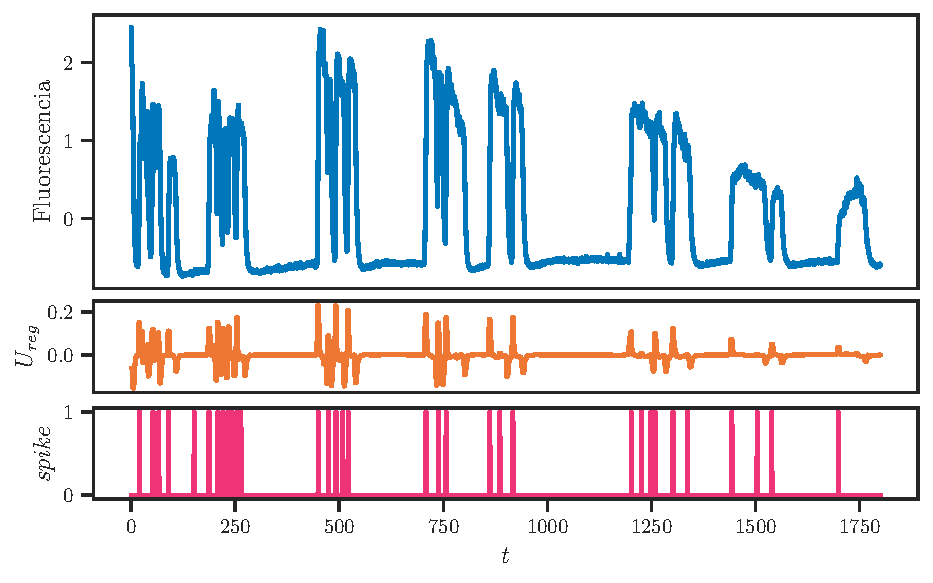
\includegraphics[width=\imsize]{kaplan_derivada.pdf}
	\caption[Inferencia de la actividad de spikes con el método de picos.]{Inferencia de la actividad de spikes con el método de picos.  trazas de calcio ($\Delta F/F$, azul), derivada regularizada (naranja) y spikes discretas inferidas de la derivada regularizada (rosado), se  destaca la eliminación de ruido a través de la inferencia de spikes.}\label{f:resultado_picos}  
\end{figure}




\subsection{CASCADE}

La idea clave en la que se basa este enfoque  de aprendizaje automático es que los datos de referencia (datos de entrenamiento) son tan importantes como el propio algoritmo y deben coincidir lo mejor posible con el nivel de ruido y la frecuencia de muestreo de los datos de imágenes de calcio de nuestros datos.  Para extraer los niveles de ruido, calculamos una métrica de ruido estandarizada $\nu$ que es robusta a los valores atípicos y aproxima la desviación estándar de las fluctuaciones de la línea de base de $\Delta F/F$
\begin{equation}
\nu = \frac{\text{Median}_t\left| \frac{\Delta F}{F}(t+1)-\frac{\Delta F}{F}(t) \right| }{\sqrt{f_r}},
\end{equation}

esta métrica se normalizó por la raíz cuadrada de la frecuencia de muestreo para permitir la comparación de las mediciones de ruido entre conjuntos de datos. En consecuencia, $\nu$ tiene unidades de  \unit{\percent \per\hertz^{-1/2}}.   La \Cref{f:nivel_ruido} muestra  el nivel de ruido $\nu$ en función del número de neuronas registradas simultáneamente en todos los experimentos considerados. Cada punto de datos representa un animal.  En el caso del conjunto de datos considerado en este apartado, el  nivel de ruido  promedio es de $1.52\pm0.45$  ( \unit{\percent \per\hertz^{-1/2}}; mediana $\pm$ s.d.) en 103 neuronas, el cual es un nivel de ruido bastante bajo. La  \Cref{f:histruido} muestra la distribución de ruido entre las neuronas de este conjunto de datos. En estas condiciones, se espera que las predicciones sean muy precisas por el algoritmo. 

    \begin{figure}[h!]
	\centering{}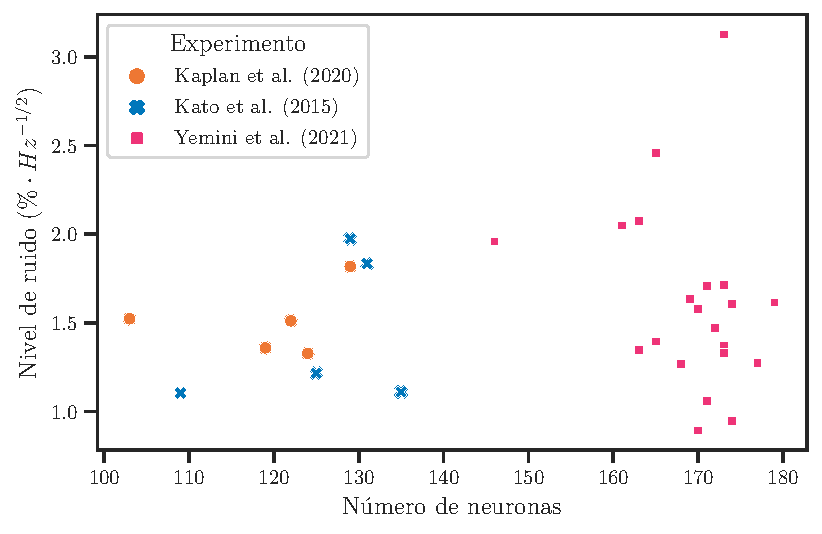
\includegraphics[width=\imsize]{nivel_ruido.pdf}
	\caption[Número de neuronas registradas en función de los niveles de ruido estandarizados.]{Número de neuronas registradas en función de los niveles de ruido estandarizados (en \unit{\percent \per\hertz^{-1/2}}) para todos los experimentos.}\label{f:nivel_ruido}  
\end{figure}



    \begin{figure}[h!]
	\centering{}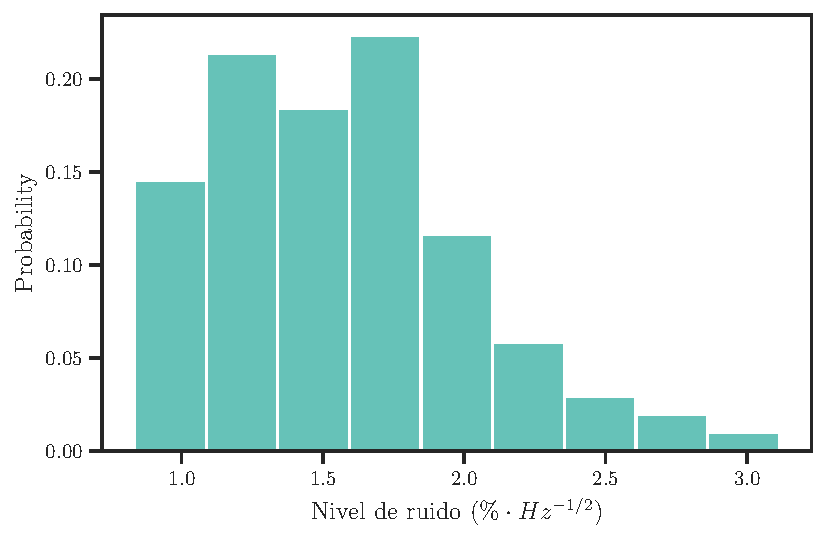
\includegraphics[width=\imsize]{histograma_ruido.pdf}
	\caption[Histograma de los niveles de ruido entre las neuronas]{Histograma de los niveles de ruido entre las neuronas
}\label{f:histruido}  
\end{figure}

A continuación, se buscó    el modelo preentrenado  de CASCADE que mejor se adapte a los datos. En nuestro caso como no tenemos una verdad fundamental específica para el conjunto de datos,  utilizamos un modelo que ha sido entrenado en todos los conjuntos de datos disponibles (llamado \textquote{Modelo Global EXC}).   Este modelo está entrenado en un conjunto de datos de verdad fundamental remuestreado. El conjunto de datos de entrenamiento se remuestrea a la frecuencia de muestreo deseada y a múltiples niveles de ruido. El modelo elige automáticamente el modelo con los niveles de ruido coincidentes para cada neurona. Solo se tiene  que seleccionar la frecuencia de muestreo correcta (que se indica en el nombre del modelo). En nuestro caso la frecuencia de muestro es \qty{3}{\hertz}.  Ademas existen  dos especificaciones del modelo adicionales que se pueden elegir: núcleos \textquote{causales} y \textquote{suavizados}.  El mas adecuado a nuestros datos es el núcleo casual ya que   la actividad de spikes se asigna casi exclusivamente a puntos de tiempo posteriores al inicio del evento de calcio. 

Por lo tanto utilizando el modelo   \textbf{ Global EXC 3Hz smoothing400ms causalkernel}, estimamos las tasas de spikes  de las 103 neuronas. La \Cref{f:cascade_spikes} destaca cómo el algoritmo de inferencia de spikes puede eliminar el ruido de las trazas de calcio. Esto se puede observar comparando las trazas de calcio sin procesar (azul) con las tasas de spikes inferidas (naranja). Las tasas de spikes inferidas son mucho más suaves y menos ruidosas que las trazas de calcio sin procesar. Para obtener eventos de spikes discretos a partir de las probabilidades inferidas, se aplicó un umbral para binarizar estas probabilidades. Se encontró que un umbral de $0.4$ es adecuado para realizar una buena discretización. El resultado se muestra en el rasterplot de la \Cref{f:cascade_spikes}, en donde se evidencia que los tiempos de los spike  estan sincronizados con  la dinámica de la neurona.

    \begin{figure}[h!]
	\centering{}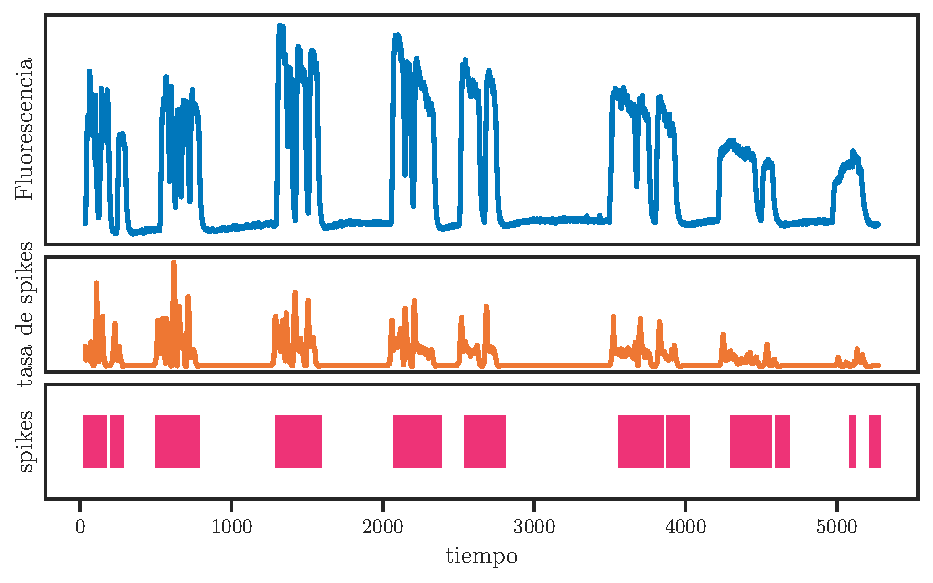
\includegraphics[width=\imsize]{cascade_spikes.pdf}
	\caption[Inferencia de la actividad de spikes con CASCADE.]{Inferencia de la actividad de spikes con CASCADE.  trazas de calcio ($\Delta F/F$, azul), tasas de spikes inferidas (naranja) y spikes discretas inferidas (rosado), se  destaca la eliminación de ruido a través de la inferencia de spikes.}\label{f:cascade_spikes}  
\end{figure}

Ademas los datos $\Delta F/F$ sin procesar a menudo también presentaban ruido correlacionado, visible como una franja vertical ruidosa en los gráficos de matriz, que era pequeño para las neuronas individuales pero tendía en algunos conjuntos de datos a dominar el $\Delta F/F$ medio entre las neuronas, posiblemente debido al ruido técnico. CASCADE eliminó visiblemente estos artefactos (\Cref{f:cascade_2}). Este ejemplo ilustra cómo la inferencia de spikes calibrada por CASCADE puede aplicarse para eliminar el ruido de las señales de calcio y para analizar la estructura temporal de la dinámica de las poblaciones neuronales. 


    \begin{figure}[h!]
	\centering{}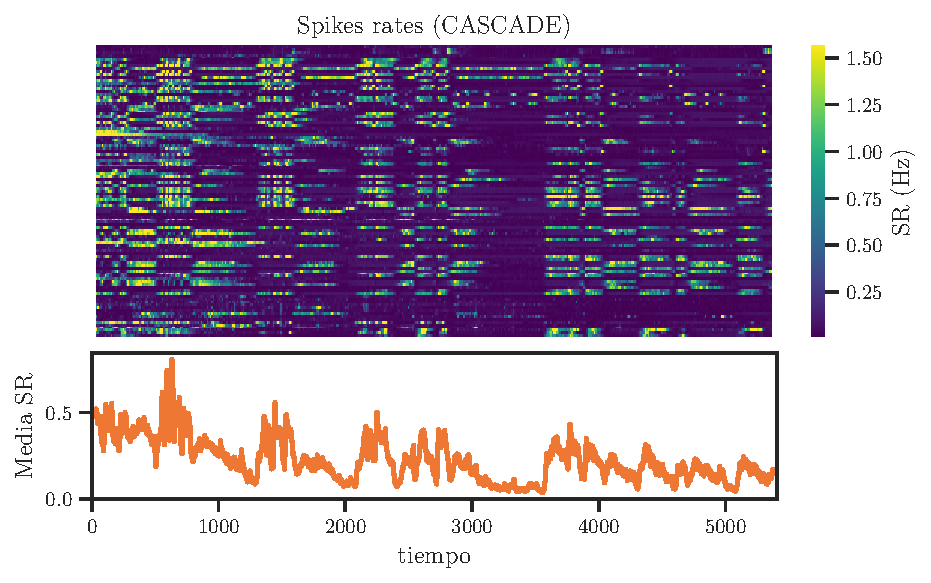
\includegraphics[width=\imsize]{cascade_2.pdf}
	\caption[Tasas de spikes inferidas con CASCADE  del conjunto de datos RIShisCl  (gusano 1).]{Tasas de spikes inferidas con CASCADE  del conjunto de datos RIShisCl  (gusano 1). El ruido se redujo por parte del algoritmo.}\label{f:cascade_2}  
\end{figure}

  
\subsection{Patrones de actividad neuronal observados}


Se utilizaron los anteriores algoritmos   para inferir los spikes de las 103 neuronas registradas simultáneamente del gusano 1 del conjunto de datos RIShisCl del experimento de Kaplan.  La \Cref{f:cascade_1} muestra las señales de calcio  sin procesar. Las franjas verticales recurrentes visibles a nivel global  marcan la presencia de actividad de red correlacionada, en consonancia con la presencia de oscilaciones colectivas  (estados ascendentes y descendentes) que se sabe que ocurren en diversas circunstancias en la dinámica neuronal espontanea. 


    \begin{figure}[h!]
	\centering{}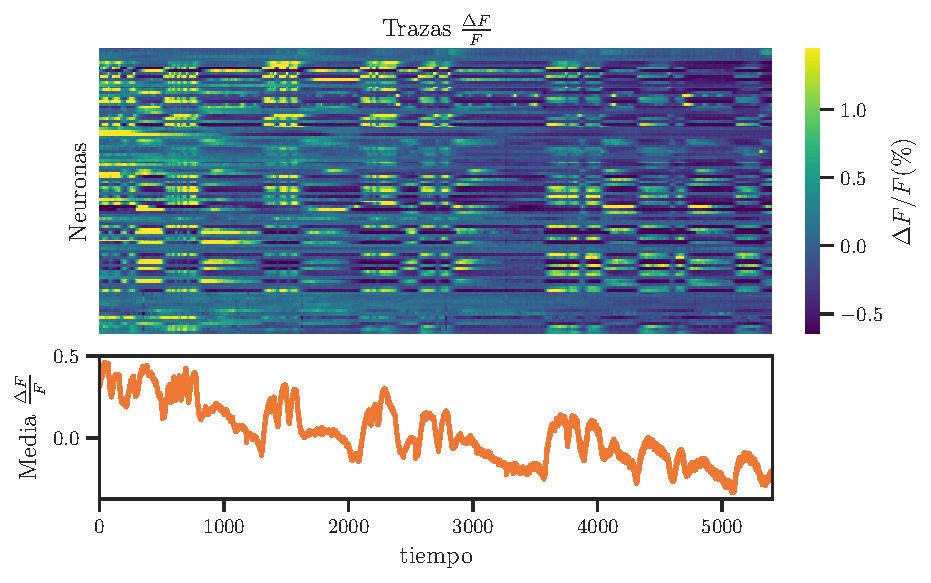
\includegraphics[width=\imsize]{cascade_1.pdf}
	\caption[Trazas $\Delta F/F$ sin procesar  del conjunto de datos RIShisCl  (gusano 1).]{Trazas $\Delta F/F$ sin procesar  del conjunto de datos RIShisCl  (gusano 1).  Las franjas verticales recurrentes visibles a nivel global  marcan la presencia de actividad de red correlacionada.}\label{f:cascade_1}  
\end{figure}



Al aplicar los algoritmos anteriormente descritos se obtienen los resultados mostrados en las \Cref{f:oasis_spike,f:MCMC_spike,f:kaplan_raster,f:cascade}.   El algoritmo OASIS (\Cref{f:oasis_spike}) muestra claras diferencias en la actividad de red correlacionada  con respecto a las  trazas de fluorescencia    (\Cref{f:cascade_1}). Esto puede deberse a que el algoritmo no hace una inferencia a nivel poblacional y por tanto puede ser sensible  a artefactos de ruido de neuronas individuales que hace que parte de la sincronización a nivel temporal se pierda.  En el caso de el algoritmo MCMC (\Cref{f:MCMC_spike})  el resultado es mas consistente con la dinámica	 real de los datos, esto se debe a que este algoritmo  realiza muestreos estocásticos aumentando la calidad de la inferencia, la desventaja de este tipo de algoritmos es su alto costo computacional. Por otro lado el método de Kaplan (\Cref{f:kaplan_raster}) muestra una característica deseable de los spikes la  escasez de picos (spike sparsity) de la actividad neuronal, el problema es que algunas dinámicas de baja frecuencia pueden perderse por este método.   Finalmente  en comparación con los otros enfoques, las predicciones de spikes  de CASCADE fueron más precisas (\Cref{f:cascade}). Se logro encontrar la presencia de actividad de red correlacionada tal como en los datos reales.   La comparación de las señales $\Delta F/F$ y  los spikes inferidos mostró que CASCADE detectó fases de actividad, pero suprimió de forma efectiva las fluctuaciones irregulares pequeñas en las trazas de actividad, lo que indica que la inferencia de spikes suprimió el ruido. 

 \begin{figure}[h!]
	\centering{}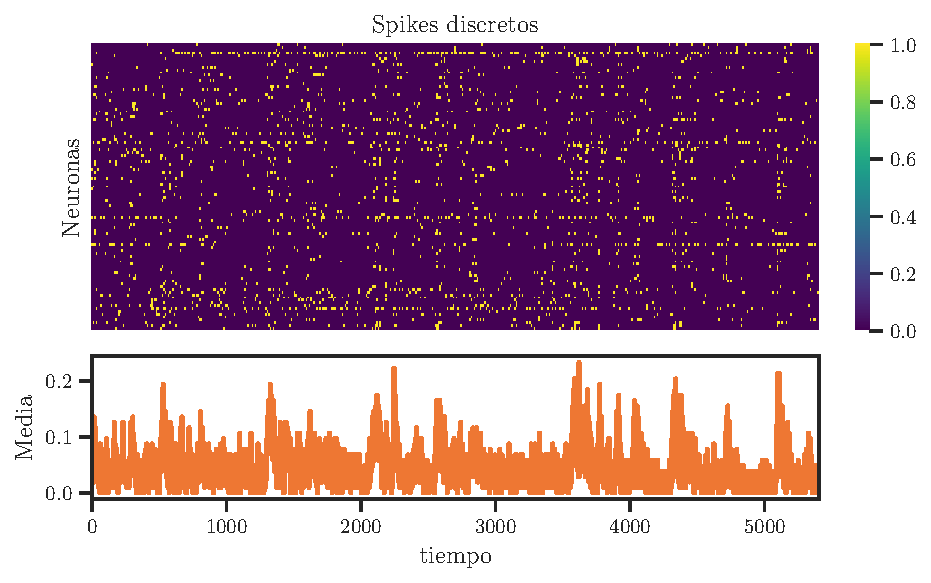
\includegraphics[width=\imsize]{oasis_spike.pdf}
	\caption[Representación  matricial de los spikes de las 103 neuronas obtenidas con OASIS. ]{Representación  matricial de los spikes de las 103 neuronas obtenidas con OASIS.}\label{f:oasis_spike}  
\end{figure}

\begin{figure}[h!]
	\centering{}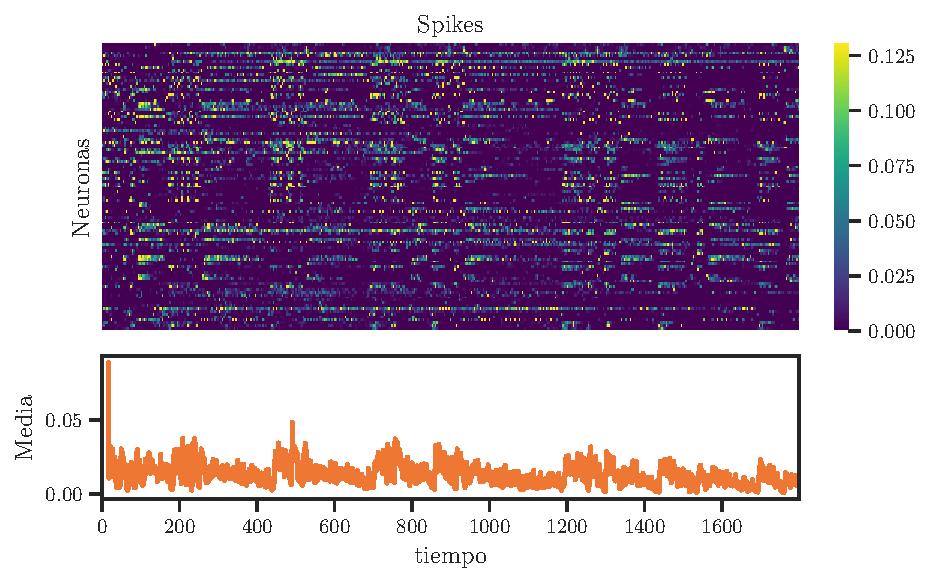
\includegraphics[width=\imsize]{MCMC_spike.pdf}
	\caption[Representación  matricial de los spikes de las 103 neuronas obtenidas con MCMC. ]{Representación  matricial de los spikes de las 103 neuronas obtenidas con MCMC. La matriz muestra  actividades correlacionadas en la red (que aparecen como alineaciones verticales de spikes).}\label{f:MCMC_spike}  
\end{figure}


\begin{figure}[h!]
	\centering{}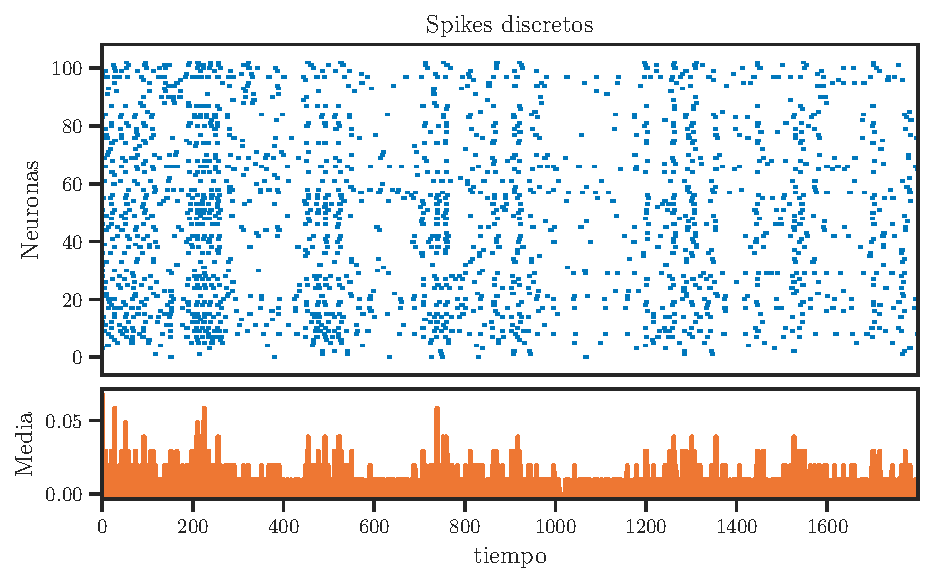
\includegraphics[width=\imsize]{kaplan_raster.pdf}
	\caption[Representación  matricial de los spikes de las 103 neuronas obtenidas con el método de Kaplan et al. ]{Representación  matricial de los spikes de las 103 neuronas obtenidas con el método de Kaplan et al. La matriz muestra  actividades correlacionadas en la red (que aparecen como alineaciones verticales de spikes).}\label{f:kaplan_raster}  
\end{figure}

\begin{figure}[h!]
	\centering{}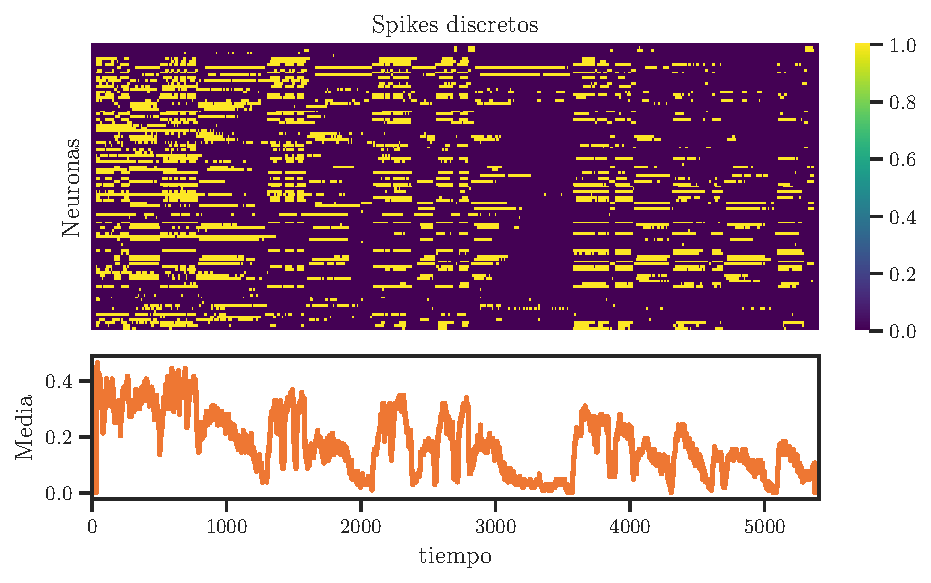
\includegraphics[width=\imsize]{cascade_3.pdf}
	\caption[Representación  matricial de los spikes de las 103 neuronas obtenidas con CASCADE. ]{Representación  matricial de los spikes de las 103 neuronas obtenidas con CASCADE. La matriz muestra  actividades correlacionadas en la red (que aparecen como alineaciones verticales de spikes).}\label{f:cascade}  
\end{figure}



\subsection{Discusión}

Estamos interesados en los grupos de neuronas coactivos y contiguos. Para ello, primero buscamos inferir  la actividad de cada una de las neuronas umbralizando las fluctuaciones de intensidad de fluorescencia $\Delta F/F$.  Para realizar esta umbralizacion  nos basamos  en tres algoritmos disponibles en la literatura: métodos auto-regresivos AR(p), métodos de inferencia bayesiana y métodos de aprendizaje profundo.  Los enfoques bayesianos  (MCMC)   superaron a los métodos auto-regresivos AR(p)  (OASIS) tanto en la estimación de tasas de spike como en la actividad global de red coordinada. Curiosamente, el algoritmo MCMC  devuelve trenes de spikes de muestra reales que pueden utilizarse, por ejemplo, para investigar las propiedades de la red en función de los tiempos de los spikes. Al mismo tiempo, MCMC devuelve muchos de estos trenes de spikes, muestreados según la distribución de probabilidad posterior, lo que permite tanto la estimación de las probabilidades de spikes como una indicación del nivel de incertidumbre de la estimación \cite{deneux_accurate_2016}. 

CASCADE funcionó mejor que todos los demás métodos en la mayoría de los casos. El método  puede inferir  los spikes con alta precisión, incluso a niveles de SNR bajos. Esto sugiere que CASCADE puede utilizarse para analizar datos de imágenes de calcio de poblaciones muy grandes de neuronas. Por lo que  en comparación con los otros enfoques estudiados en este apartado, las predicciones de la actividad global correlacionada   de CASCADE fueron más precisas, pero también menos sesgadas hacia subestimaciones de los spikes reales tal como el algoritmo OASIS (\Cref{f:oasis_spike}). En segundo lugar, dado que no se  necesita ajustar los hiperparámetros, la aplicación de la inferencia de spikes se vuelve sencilla en la práctica. Estos resultados sugieren que CASCADE es un método robusto y confiable para la inferencia de spikes en una amplia gama de condiciones experimentales. Por lo tanto en conjunto, estos aspectos reflejan que, a diferencia de los algoritmos basados en modelos, CASCADE puede hacer uso de conjuntos de datos de referencia de manera eficiente y natural. Por lo que en el resto de este documento utilizamos CASCADE para  la inferencia de los spikes de la  dinámica global de todos los experimentos.

  
 
 \section{Clústeres de actividad neuronal}\label{sec:actividad_neuronal_experimento}
 
 
 
En este apartado, caracterizamos los patrones espaciales de la actividad neuronal colectiva calculando el número de clústeres y su distribución de tamaños (número de activaciones; ver \cref{sec:clusteres}) en los datos experimentales. Estudiamos las estadísticas de los clústeres en el marco de la teoría de la percolación. Como se discutió en el \cref{sec:cap-percolacion}, la percolación describe el comportamiento de los clústeres en un grafo y cómo cambian los tamaños de los clústeres con el número de unidades activas, pasando de pequeños clústeres a la aparición de un gran clúster más allá de un nivel crítico de actividad \cite{rocha_recovery_2022}. A lo largo de este estudio, analizamos la actividad espontánea.
 
 \subsection{Correlación entre actividades neuronales}\label{sec:correlacion}
 
 Antes de abordar la caracterización de los clústeres neuronales de la actividad neuronal de los experimentos con C. elegans vamos a detallar varias características destacadas en estas series temporales. Para visualizar mejor los grupos de neuronas que comparten actividad en  las series temporales, se aplico a los conjuntos de datos un algoritmo de clustering jerárquico/aglomerativo mediante la función de seaborn  \textbf{clustermap}\footnote{https://seaborn.pydata.org/generated/seaborn.clustermap.html} (  \Cref{fig:seriedatos}).  En primer lugar, existen grupos de neuronas  que mostraron activación e inactivación sincronizadas. Dado que no existe estimulación en los datos de Kaplan et al. y Kato et al. este comportamiento se considera como  actividades espontáneas. Estas observaciones son consistentes con lo reportado por Kat et al. \cite{kato_global_2015}. Para aclarar aún más esto, se determinaron las correlaciones cruzadas en las actividades neuronales utilizando el metodo de correlación de Pearson 
 en todas las combinaciones de neuronas por pares (\Cref{fig:correlaciones_experimentos}). Se observó que el tamaño de cada grupo correlacionado difería considerablemente entre los distintos conjuntos de datos. Aquí, también es evidente que en muchos casos, en cada conjunto  hay al menos un grupo principal de neuronas con actividad correlacionada, y a menudo hay otro grupo correlacionado que está correlacionado negativamente con el primer grupo. Al detallar las  neuronas miembro por ejemplo en el conjunto de Yemini et al se revela que estos grupos corresponden a los grupos bien conocidos de neuronas relacionadas con los movimientos de retroceso y avance de los animales, a saber, las neuronas AVA, AVE y RIM, etc. en el primer grupo (las correlaciones son por ejemplo: (AVAR,AVAL): 0.942, (AVAL,AVER): 0.8941, (AVAL,RIMR): 0.8911 ), y las neuronas RIB, RID y RME, etc. en el segundo grupo ((RIBL,RID): 0.918, (RIBL,RMEL): 0.5181, (RID,RMER): 0.46). Otros grupos que se correlacionaron entre los datos incluyeron  [(OLLL,OLLR): 0.96, (OLLL,OLQDL): 0.82, (OLQDL, OLQDR): 0.582 ]  y [(I2L,I2R): 0.97, (I2L,MCL): 0.9963, (I2R,MCL): 0.971]     , y  [(BAGL,BAGR): 0.72, (RIAL,RIAR): 0.52, (RMDVL,RMDVR): 0.667, (SMDDL,SMDDR): -0.51] \cite{toyoshima_deducing_2022}. Es importante destacar  que la correlación entre la actividad de estos grupos era consistente en diferentes muestras de gusanos de los distintos experimentos.
 

 
  \begin{figure}
 	\centering
 	\begin{subfigure}[b]{0.3\textwidth}
 		\centering
 		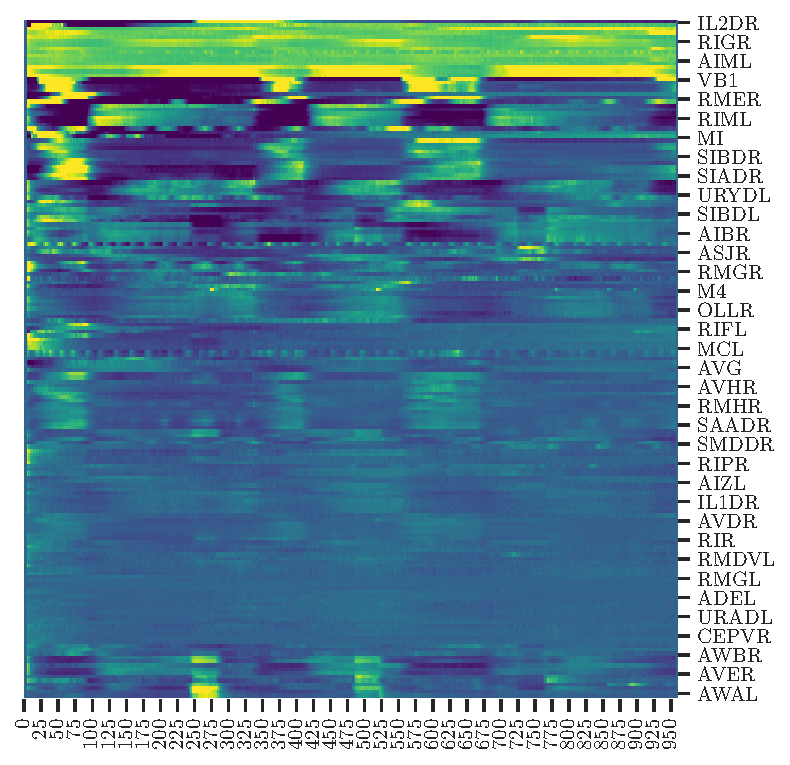
\includegraphics[width=\textwidth]{cluster_neuropal.pdf}
 		\caption{}
 		\label{fig:cluster_neuropal}
 	\end{subfigure}
 	\begin{subfigure}[b]{0.3\textwidth}
 		\centering
 		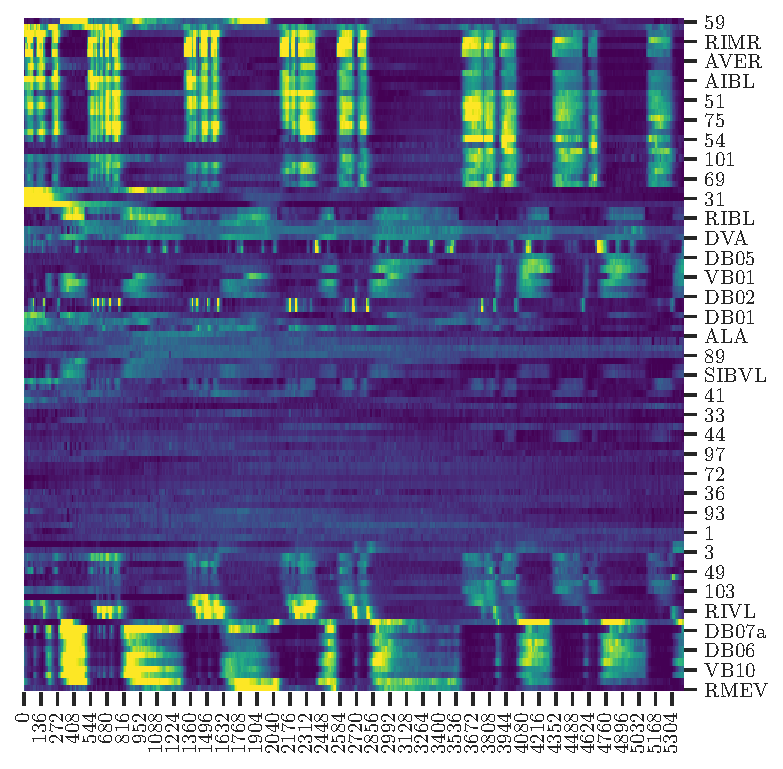
\includegraphics[width=\textwidth]{cluster_kaplan.pdf}
 		\caption{}
 		\label{fig:cluster_kaplan}
 	\end{subfigure}
 	\begin{subfigure}[b]{0.3\textwidth}
 		\centering
 		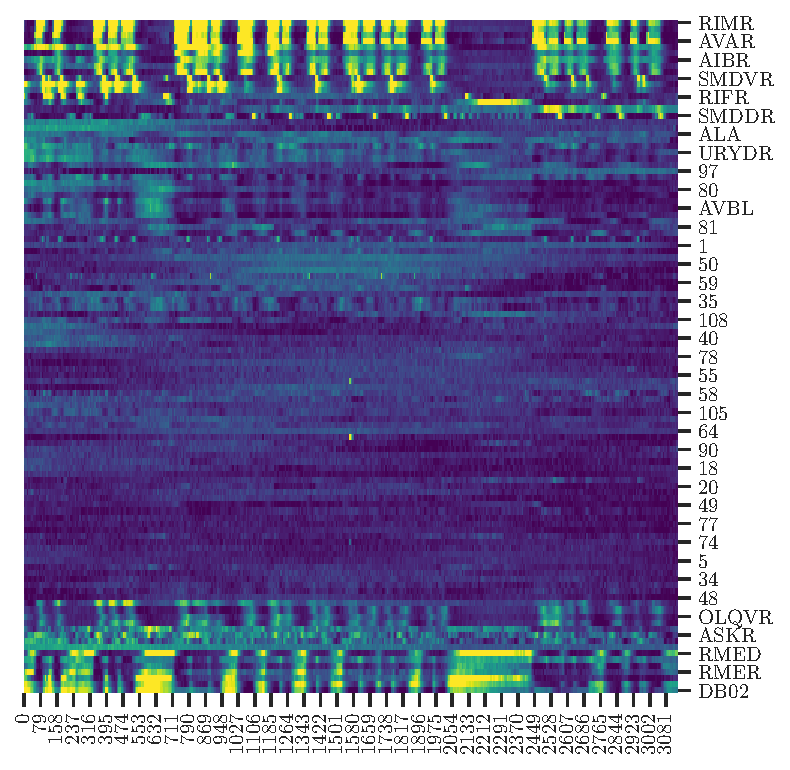
\includegraphics[width=\textwidth]{cluster_kato.pdf}
 		\caption{}
 		\label{fig:cluster_kato}
 	\end{subfigure}
 	\caption[Serie temporal de actividad de las neuronas del primer gusano en cada conjunto de datos.]{ Serie temporal de actividad de las neuronas del primer gusano en cada conjunto de datos. Cada fila representa una neurona, cuyo orden se determinó mediante agrupamiento jerárquico. (a) Yemini et al. (b) Kaplan et al. (c) Kato et al.}\label{fig:seriedatos}
 \end{figure}
 
 \begin{figure}[h!]
\centering
 	 	\begin{subfigure}[b]{0.3\textwidth}
	\centering
	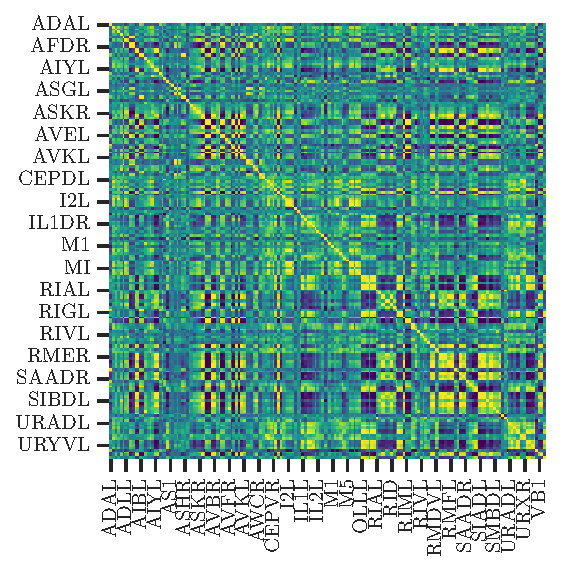
\includegraphics[width=\textwidth]{correlacion_neuropal.pdf}
	\caption{}
	\label{fig:correlacion_neuropal}
\end{subfigure}
\begin{subfigure}[b]{0.3\textwidth}
	\centering
	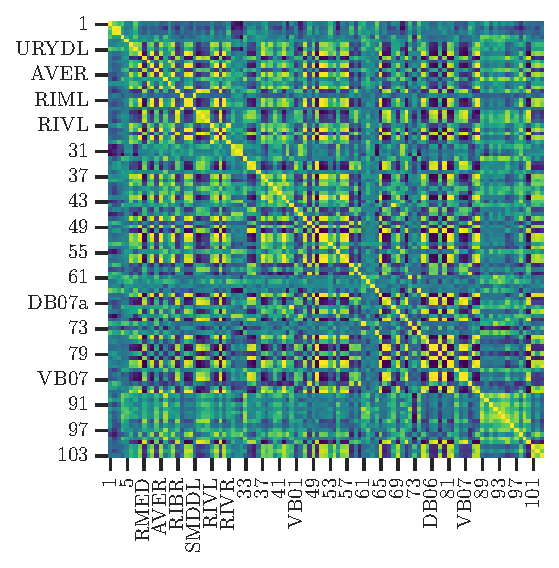
\includegraphics[width=\textwidth]{correlacion_kaplan.pdf}
	\caption{}
	\label{fig:correlacion_kaplan}
\end{subfigure}
\begin{subfigure}[b]{0.3\textwidth}
	\centering
	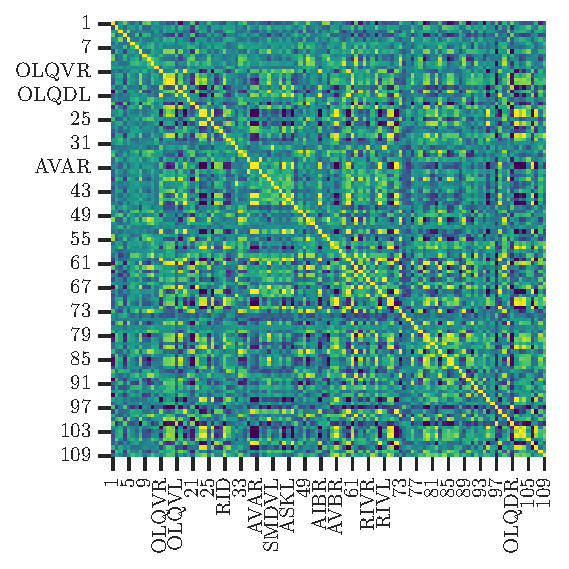
\includegraphics[width=\textwidth]{correlacion_kato.pdf}
	\caption{}
	\label{fig:correlacion_kato}
\end{subfigure}
\caption[Correlación cruzada por pares de las actividades de las neuronas  del primer conjunto de datos de los experimentos con C elegans.]{Correlación cruzada por pares de las actividades de las neuronas  del primer conjunto de datos de los experimentos con C elegans. (a)  Yemini et al. (b) Kaplan et al. (c) Kato et al. El color amarillo muestra una correlación positiva y el color azul muestra una correlación negativa.} \label{fig:correlaciones_experimentos}
 \end{figure}
 
 
 

 
 
 
 \subsection{Calculo de distribución de clústeres red cuadrada}\label{eq:redcuadarda_clusteres}
 
 Antes de encontrar la distribución de los tamaños de los clústeres de los datos experimentales,   corroboraremos el buen funcionamiento del algoritmo  descrito en el  \cref{sec:alg_cluster}. Para este fin,  utilizaremos la red cuadrada como  modelo de control.  La ventaja de este modelo es que tanto la   distribución de clústeres  y sus propiedades estadísticas están disponibles  en la literatura, por lo que podemos compararlos con los resultados del  algoritmo.   Generamos  una red de puntos $L\times L$ que están ocupados con probabilidad $p$.   La matriz resultante se ilustra en la \Cref{f:matriz_clusteres}(a). Sin embargo, esta visualización no nos proporciona ninguna información sobre la conectividad de los sitios en este sistema. En su lugar, analizamos las regiones conectadas en el sistema. Para encontrar las regiones conectadas utilizamos el algoritmo descrito en el  \cref{sec:alg_cluster}. Tanto para este ejemplo como para los resultados experimentales y el modelo  de criticidad neuronal utilizamos la funcion de Scipy \textbf{sparse.csgraph.connected\_components}\footnote{\url{https://docs.scipy.org/doc/scipy/reference/generated/scipy.sparse.csgraph.connected_components.html}} para analizar los componentes conectados de un grafo cuya entrada es  la matriz de adyacencia del grafo.  Ademas como deseamos calcular las componentes débilmente conexas utilizamos el valor \textquote{weak} del parámetro  connection. 
 
 \begin{figure}[h!]
 	\centering{}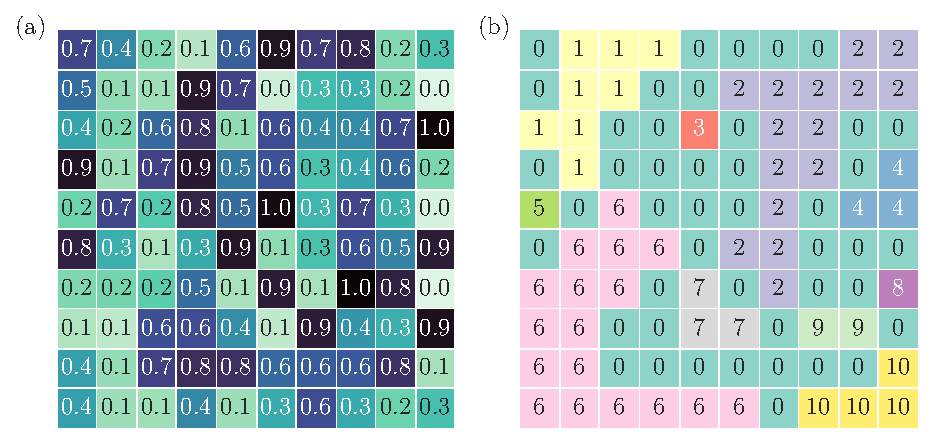
\includegraphics[width=\imsize]{matriz_clusteres.pdf}
 	\caption[ Ilustración de una matriz de números aleatorios de $10\times10$, y los diversos sitios establecidos para $p=0.45$. ]{ Ilustración de una matriz de números aleatorios de $10\times10$, y los diversos sitios establecidos para $p=0.45$. (a) Ilustración de una matriz de números aleatorios de $10\times10$ . (b) Ilustración de la matriz de índices  para $p = 0.45$.}\label{f:matriz_clusteres}  
 \end{figure}

 Esta función devuelve la matriz de etiquetas, que para cada nodo en la matriz de adyacencia original indica a qué clúster pertenece. Los clústeres se numeran secuencialmente y a cada clúster se le asigna un índice. Todos los nodos con el mismo índice pertenecen al mismo clúster. La matriz resultante se muestra en la \Cref{f:matriz_clusteres}(b), donde se muestra el índice para cada sitio y se utiliza un color para indicar los diversos clústeres. 
 
 \subsubsection{Distribución del numero de clústeres}
 
  Para comprender mejor la distribución de los tamaños de los clústeres, estudiemos la \Cref{f:matriz_clusteres} con más detalle.  Hay 3 clústeres de tamaño $s = 1$, un clúster de tamaño $s = 2$, 2 clústeres de tamaño $s=3$ y 1 clústeres de tamaño $s=4$, $s=8$, $s=15$ y $s=17$ respectivamente.   Tal como se describió en el \Cref{sec:medicion_clusteres}  
mediante  un histograma de tamaños de clústeres podemos encontrar la distribución de clústeres numéricamente.  Para los clústeres en la  \Cref{f:matriz_clusteres}   la estimación de $\overline{n(s, p;L)}$ (\Cref{eq:88}) basada en esta única realización se resume  en el \cref{table:histograma_cluster}. 
 \begin{table}[h!]
	\centering
	\caption[Histograma de tamaños de clústeres]{ Histograma de tamaños de clústeres.}
	\begin{tblr}{colspec={llllllll},
			row{odd} = {bg=gray8},
			row{even} = {bg=gray9},
			column{1} = {bg=red3, fg=white, font=\sffamily},
		}
		
		$s$ & 1 & 2 & 3 & 4 &     8 &15 & 17 \\
		$Ns$ & 3 & 1 & 2 & 1 &   1 & 1  & 1\\
		$n(s,p)$ & 3/100 & 1/100 & 2/100 & 1/100   & 1/100 &  1/100 &  1/100\\
	\end{tblr}
	\label{table:histograma_cluster}
\end{table}

Teniendo en cuenta lo anterior se simulo una red cuadrada con  $L=1000$. Para producir buenas estimaciones estadísticas de $n(s, p)$ se realizaron $M=1000$  realizaciones aleatorias del sistema. Estimamos $\overline{n(s, p; L)}$ utilizando la  \Cref{eq:88} para $p=0.57$, el resultado se muestra en la  \Cref{f:num_clusteres_red_cuadrada}a,b.    Desafortunadamente, este gráfico no es muy útil. El problema es que hay muchos valores de $s$ para los que tenemos pocos o ningún dato. Para los valores pequeños de $s$ tenemos muchos clústeres para cada valor de $s$ y las estadísticas son buenas. Pero para los valores grandes de $s$, tenemos menos de un punto de datos para cada valor de $s$. Por lo tanto, nuestra distribución medida $\overline{n(s, p; L)}$ es una mala representación de la $n(s, p; L)$ real en este rango.

El problema con los resultados medidos en la  \Cref{f:num_clusteres_red_cuadrada}a,b ocurre porque hemos elegido un tamaño de bin muy pequeño para el histograma. Sin embargo, vemos que para valores pequeños de $s$ queremos tener un tamaño de bin pequeño, ya que las estadísticas aquí son buenas, pero para valores grandes de $s$ queremos tener tamaños de bin más grandes. Esto a menudo se resuelve utilizando un binning logarítmico.  El gráfico resultante  se muestra en la \Cref{f:num_clusteres_red_cuadrada}c. Observase que el gráfico resultante ahora es mucho más fácil de interpretar que el gráfico binneado linealmente.  Por lo tanto, en lo siguiente adaptaremos estrategias de binning logarítmico siempre que midamos un conjunto de datos que es escaso.



\begin{figure}[h!]
	\centering{}\includegraphics[width=\imsize]{num_clusteres_red_cuadrada.pdf}
	\caption[Gráfico de $n(s, p; L)$ estimado a partir de $M = 1000$ muestras para  $p=0.57$ y $L = 1000$.]{Gráfico de $n(s, p; L)$ estimado a partir de $M = 1000$ muestras para $p=0.57$ y $L = 1000$. (a) Gráfico directo. (b) Gráfico log-log. (c) Gráfico de la distribución agrupada logarítmicamente.}\label{f:num_clusteres_red_cuadrada}  
\end{figure}


\subsubsection{Mediciones de $n(s, p)$ cuando $p \to p_c$}\label{sec_critico}

¿Qué sucede con $n(s, p;L)$ cuando cambiamos $p$ para que se acerque a $p_c$? Realizamos una secuencia de simulaciones para varios valores de $p$ para la red anteriormente simulada y trazamos los valores resultantes para $\overline{n(s, p; L)}$. El gráfico resultante se muestra en la \Cref{f:num_cluster_critico}. Dado que el gráfico es doblemente logarítmico, una línea recta corresponde a un comportamiento de tipo ley de potencia, $n(s, p) \propto s^{-\tau}$.  En el caso de una red cuadrada bidimensional el valor del umbra critico es $p_c\approx0.592746$ (ver \Cref{table:umbral}), que en la  \Cref{f:num_cluster_critico} es la linea roja. Esto  sugiere que en este valor de $p$ el algoritmo que calcula la distribución de clústeres da un comportamiento que puede describirse mediante una ley de potencia, tal como se esperaba. Como se discutió en  el \cref{sec:leypotencia_intro}   el  hecho que un histograma de la ley de potencias presente una relación lineal en un gráfico doblemente logarítmico es una condición necesaria pero no suficiente para decir que los datos siguen una distribución de tipo ley de potencia. Por lo que la inspección visual de un diagrama puede generar falsos positivos.  Sumado a esto  ajustar con precisión una distribución de ley de potencia a datos empíricos, así como medir la bondad de ese ajuste, no es trivial. Para solventar estas dificultades aplicamos los métodos descritos en el \cref{sec:leypotencia} tanto para ajustar y evaluar distribuciones de colas pesadas en los datos. La implementación del algoritmo LSavg en Python se encuentra disponible en el repositorio de GitHub  de los autores \url{https://github.com/xszhong/LSavg/tree/main}.  


\begin{figure}[h!]
	\centering{}\includegraphics[width=\imsize]{num_cluster_critico.pdf}
	\caption[Gráfico de $n(s, p; L)$ en función de $s$ para varios valores de $p$ para una red de $1000\times1000$.]{Gráfico de $n(s, p; L)$ en función de $s$ para varios valores de $p$ para una red de $1000\times1000$.}\label{f:num_cluster_critico}  
\end{figure}



Para comprobar el funcionamiento del método de ajuste de leyes de potencia, se simularon $M=1000$ realizaciones  aleatorias de    una red cuadrada con  $L=1000$ y $p=p_c\approx0.592746$. Las estimaciones estadísticas de $n(s, p)$  
se agrupan mediante un conjunto de puntos de datos $\left\{\left(x_i,f(x_i)\right)\right\}$ en orden ascendente por sus valores $x$, donde $f(x_i)$ es la frecuencia de $x_i$ en la muestra. Ademas establecemos cuatro puntos de datos críticos cuyos valores de $x$ son $X_{5th}$ , $X_f$ , $X_1$ , $X_{max}$.  Por conveniencia, usamos los cuatro valores críticos de $x$ para representar sus puntos de datos correspondientes y los usamos con llaves para representar el subconjunto de puntos de datos desde el primer punto de datos hasta ellos; por ejemplo, $\{ X_{5th}\}$ representa el conjunto de los primeros cinco puntos de datos mientras que $\{ X_1 \}$ representa el conjunto de puntos de datos desde el primero hasta $X_1$. Las definiciones de estos puntos de datos críticos son las siguientes. $X_{5th}$ indica el quinto punto de datos. $X_f$ indica el último punto de datos en el que todos los puntos de datos de $\{ X_f \}$ satisfacen la propiedad  estrictamente decreciente del punto de datos ; mientras que su primer punto de datos posterior no satisface  esta  propiedad. $X_1=\min\left\{x_i\mid f(x_i)=\frac{1}{n}\right\}$ indica el primer punto de datos cuya frecuencia es $1/n$. $X_{max} = \max\left\{x_i\right\}$ indica el último punto de datos. Según las definiciones anteriores, la relación entre ellos es $X_f \leq  X_1 \leq X_{max}$.


Supongamos que el muestreo es perfecto (lo que significa que los datos muestreados siguen perfectamente una distribución de ley de potencia), la frecuencia del punto de datos de menor frecuencia es $1/n$ y sea este punto de datos $(X^T_1,1/n)$ entonces resolviendo $p(X^T_1)=K\cdot1/n$, obtenemos $X^T_1=(K\cdot n)^{1/\alpha}$. Esto significa que $X^T_1\propto n^{1/\alpha}$, y cuando $n \to\infty, X^T_1\to\infty$ \cite{zhong_is_2022}. Si el muestreo es perfecto, entonces $X_f=X_1=X^T_1=X_{max}$ según sus definiciones. Sin embargo, para una muestra de tamaño finito, el muestreo no es perfecto en la realidad y estos valores críticos no son iguales. Su relación empírica es $X_f<X_1<X^T_1\ll X_{max}$.



El resultado se muestra en la \Cref{f:ley_potencia_red_cuadrada}.  El \cref{table:valoresalpha_redcuadrada}  reporta el resultado de aplicar LSE para ajustar los datos discretos.  $\hat{\alpha}_{5th},  \hat{\alpha}_{f}, \hat{\alpha}_{X1}$ y $\hat{\alpha}_{all}$ indican el  $\hat{\alpha}$  ajustado por $LS_{norm}$ en $\{X5th\}, \{X_f\}, \{X_1\}$, y $\{X_{max}\}$, respectivamente. Mientras los que contienen el súper indice $avg$   indican el  $\alpha$ ajustado por $LS_{avg}$ en los puntos de datos correspondientes.   El \cref{table:valoresalpha_redcuadrada}   muestra  que  $\alpha_{all}$ tiene un valor de $0.7802$, lo que supone un sesgo significativo con respecto al valor real de $36/91$ reportado en la literatura (ver \Cref{table:exponentepercolacion} ).  Esta estimación sesgada es consistente con la reportada por los críticos de los métodos LSE. El mal resultado de este ajuste se debe a que se incluyen los ruidos de cola larga, los cuales no pueden tratarse como datos de ley de potencia.






\begin{figure}[h!]
	\centering{}\includegraphics[width=\imsize]{ley_potencia_red_cuadrada.pdf}
	\caption[Métodos LSE  aplicados a la distribución de tamaños de clústeres $n(s,p$) para la red cuadrada para $L=1000$ y $M=1000$ realizaciones aleatorias.]{Métodos LSE  aplicados a la distribución de tamaños de clústeres $n(s,p$) para la red cuadrada para $L=1000$ y $M=1000$ realizaciones aleatorias. $LS_{all}$ indica la aplicación de $LS_{norm}$ a todos los datos para estimar $\alpha$. $LS_{X5th}$ indica la aplicación de $LS_{avg}$ a $\{X_{5th}\}$ para estimar $\alpha$; $LS_{Xf}$ aplica $LS_{avg}$ a $\{X_f\}$; y $LS_{X1}$ aplica $LS_{avg}$ a $\{X_1\}$. $X_1^T=\left(\hat{K}\cdot n\right)^{1/\hat{\alpha}}$ es el valor $x$ de  $(X^T_1,1/n)$ donde $n$ es el tamaño de la muestra.}\label{f:ley_potencia_red_cuadrada}  
\end{figure}




	


\begin{table}[h!]
	\centering
	\caption[Estimación de $\alpha$ para el ajuste de  la distribución de tamaños de clústeres $n(s,p$) para la red cuadrada para $L=1000$ y $M=1000$ realizaciones aleatorias.]{Estimación de $\alpha$ para el ajuste de  la distribución de tamaños de clústeres $n(s,p$) para la red cuadrada para $L=1000$ y $M=1000$ realizaciones aleatorias.}
	\begin{tblr}{colspec={lllllll},
			row{odd} = {bg=gray8},
			row{even} = {bg=gray9},
			row{1} = {bg=red3, fg=white, font=\sffamily},
		}
		
		$\hat{\alpha}_{5th}$ &  $\hat{\alpha}_{5th}^{avg}$ & $\hat{\alpha}_{f}$  & $\hat{\alpha}_{f}^{avg}$  & $\hat{\alpha}_{X1}$ &  $\hat{\alpha}_{X1}^{avg}$ &  $\hat{\alpha}_{all}$ \\
		
		{2.0145} &  {2.01446} & {1.8389} & {1.8388} & {1.9543} & {1.9542} & {0.7802}
		
	\end{tblr}
	\label{table:valoresalpha_redcuadrada}
\end{table}



\begin{table}[h!]
	\centering
	\caption[Estimaciones para los exponentes críticos de la teoría de percolación de varios sistemas. ]{Estimaciones para los exponentes críticos de la teoría de percolación de varios sistemas}
	\begin{tblr}{colspec={lllllllllll},
			row{odd} = {bg=gray8},
			row{even} = {bg=gray9},
			row{1} = {bg=red3, fg=white, font=\sffamily},
		}
		
		dimensión & $\beta$ & $\tau$ & $\sigma$ & $\gamma$ & $\nu$ & $D$ & $\mu$ & $D_{min}$ & $D_{max}$ & $D_B$ \\
		1 &  & 2 & 1 & 1 & 1 & &&&&&\\
		2 & 5/36 & 	187/91 & 36/91 & 43/18 & 	4/3 &	91/48 & 1.30 &	1.13 & 	1.4 & 1.6 \\
		3 & 0.41 &	2.18 & 	0.45 & 	1.80 & 	0.88 & 	2.53 & 	2.0 & 	1.34 & 	1.6 & 	1.7 \\
		4  & 0.64 & 2.31 & 	0.48 & 	1.44 & 	0.68 & 	3.06 & 	2.4 & 	1.5 & 	1.7 & 	1.9		\\
		Bethe & 	1 & 5/2 & 	1/2 & 	1 & 	1/2 & 	4 & 	3 & 	2 & 	2 & 2
	\end{tblr}
	\label{table:exponentepercolacion}
\end{table}

	Tanto $\hat{\alpha}_{5th}$,  $\hat{\alpha}_{5th}^{avg}$, $\hat{\alpha}_{f}$, $\hat{\alpha}_{f}^{avg}$, $\hat{\alpha}_{X1}$ y   $\hat{\alpha}_{X1}^{avg}$ se estiman sin  los ruidos de cola larga. Todos ellos oscilan alrededor del valor verdadero de $\alpha$.  Específicamente $\hat{\alpha}_{5th}^{avg}=2.014$ se acerca mucho más al valor verdadero.  Esto significa que, al excluir los ruidos de cola larga, $\hat{\alpha}$ cambia de significativamente sesgado a casi no sesgado. Son los ruidos de cola larga los que causan un sesgo significativo en el LSE.  Comparando los $\hat{\alpha}$ con los $\hat{\alpha}^{avg}$, podemos ver que $LS_{avg}$ funciona mucho mejor que  $LS_{norm}$.  La razón es que la estrategia de promediado utilizada en $LS_{avg}$ reduce el impacto de aquellos puntos de datos desviados de la línea de regresión. La  \Cref{f:ley_potencia_red_cuadrada}  demuestra que $LS_{avg}$ se ajusta perfectamente a los datos de la ley potencial.
	
	
	
Después de obtener los modelos de ley de potencia estimados, calculamos sus estadísticas KS correspondientes en $\{ X_1 \}$, escogemos $D_n^{X_{5th}}$ por tener el valor  mínimo de $D_n$.  Del modelo de ley de potencia estimado extraemos 500 muestras, luego calculamos $D_n^T$ por la  \Cref{eq:98} (ver \Cref{table:valoresD_redcuadrada})  y utilizamos la estrategia descrita en el \cref{procedimiento1}. En este conjunto de datos $D_n^T=0.086$ y $D_n^{X_{5th}}=0.067$ por lo que se cumple que $D_n\leq D_n^T$ entonces aceptamos la hipótesis $H_0$ de que los datos son sacados de una distribución de tipo de ley de potencia, lo que era de esperar ya que se sabe que estos datos siguen esta distribución. Lo anterior evidencia que el algoritmo esta funcionando correctamente y puede  utilizarse para ayudarnos a corroborar la hipótesis de  que los clústeres de neuronas  en los experimentos de C. elegans  siguen una ley de potencias evidenciando  un comportamiento critico. 


 \begin{table}[h!]
	\centering
	\caption[Valores máximos de $D_{n,n}$  y sus p-valores de la prueba KS de muestras extraídas del modelo de ley de potencias con $\alpha = 2.015$ y $n = 10^4$. ]{ Valores máximos de $D_{n,n}$  y sus p-valores de la prueba KS de muestras extraídas del modelo de ley de potencias con $\alpha = 2.015$ y $n = 10^4$.  El tamaño indica el número de muestras en el grupo.}
	\begin{tblr}{colspec={lll},
			row{odd} = {bg=gray8},
			row{even} = {bg=gray9},
			row{1} = {bg=red3, fg=white, font=\sffamily},
		}
		
			Tamaño & $D_{n,m}$  &  $p_{value}$  \\
             100        &  {0.069} & {0.01709} \\
             200        & {0.086}  & {0.0012} \\
             300        & {0.086}  & {0.00122} \\
             400        & {0.094}  & {0.00028} \\
             500        & {0.094} & {0.00028} \\
	\end{tblr}
	\label{table:valoresD_redcuadrada}
\end{table}

\subsection{Estadísticas de los clústeres de la actividad neuronal }\label{eq:estadistica_cllusteres}


En la parte  anterior se utilizo un modelo de control para corroborar el funcionamiento del algoritmo del calculo de clústeres y del ajustes de colas pesadas. En esta parte se estudiara los patrones de actividad espacio-temporal que emergen de la dinámica cerebral completa de los experimentos de C elegans siguiendo los métodos anteriormente descritos.  La actividad cerebral completa se caracterizó por la activación de grupos de neuronas que podían abarcar grandes partes del cerebro. Nuestro objetivo es describir las estadísticas de estos eventos.  Para ello, la actividad de cada  neurona se binarizó utilizando los métodos descritos en los \cref{sec:umbralizacion,sec:inferencia_spikes}. Para los 21 gusanos de los experimentos de Yemini et al \cite{yemini_neuropal_2021} se utilizo el método de Kaplan de inferencia de picos en la traza  $\Delta F/F$ de cada conjunto de datos. Por otro lado, en el resto de experimentos (Kato et al \cite{kato_global_2015}, Kaplan et al \cite{kaplan_nested_2020})  se utilizo el método CASCADE para la inferencia de spikes con un umbral adecuado . A continuación, identificamos grupos de neuronas coactivadas y espacialmente contiguas y cuantificamos su número, tamaño y evolución en el tiempo.


Para caracterizar los grupos de neuronas coactivadas y espacialmente contiguas se utilizó  un enfoque de modelado híbrido que combina el conectoma del C. elegans hermafrodita reconstruido por Cook et al.  \cite{cook_whole-animal_2019}  junto con   los registros   de  las  series temporales de la dinámica neuronal binarizada  de los tres experimentos   con C. elgans. Las conexiones sinápticas entre pares de neuronas en todo el sistema nervioso (connectoma) se han descrito completamente.  Una desventaja de este método, es que  solo consideramos las neuronas etiquetadas, por lo que la cantidad de series temporales usadas para los cálculos puede ser menor que la serie neuronal Completa.  En cada paso de tiempo  se agrupan los spikes de neuronas  que comparten el mismo tipo de actividad conectados siguiendo la matriz de adyacencia del conectoma de Cook y posteriormente mediante el algoritmo descrito en el \cref{sec:alg_cluster} se calcula el tamaño del clúster, el cual  es el número total de neuronas participantes.  Posteriormente para cada tiempo $t$, calculamos la proporción de neuronas activas ($\left\langle A(t) \right\rangle$), el número de clústeres ($m$) y el tamaño del $i$-ésimo clúster ($C_s(i), 1 \leq i \leq m$ ).  



En primer lugar, tal como se realizo en  \cite{ponce-alvarez_whole-brain_2018,tagliazucchi_criticality_2012} calculamos la relación entre $\left\langle A(t) \right\rangle$ y $m$ encontrando  que  siguen una relación no lineal que se asemeja a la de la percolación.  El número de clústeres alcanzaba su máximo en un nivel crítico de actividad global  $ \left\langle A(t) \right\rangle \approx 11\%$ para los experimentos de Yemini et al \cite{yemini_neuropal_2021},  un valor que denotamos como $\left\langle A(t) \right\rangle_c$ (línea  vertical discontinua rosada en la  \Cref{fig:estadisticas_clusteres_neuropal}(a)). La variabilidad de $m$ también se maximizaba a este nivel de activación.  Ademas La correlación entre el la densidad  de sitios activos (un índice de la actividad total) y el número de clústeres se invierte por encima de este umbral crítico de actividad, una característica que ya se ha descrito en otros sistemas complejos en los que alguna densidad creciente compite con la capacidad limitada. Este resultado es interesante porque sugiere que la actividad neuronal colectiva se organiza de forma más compleja en un rango intermedio de actividad neuronal. A bajos niveles de actividad, hay pocos clústeres y la actividad neuronal está muy dispersa. A altos niveles de actividad, hay un gran clúster dominante y la actividad neuronal es más homogénea. Sin embargo, a niveles de actividad intermedios, hay una mayor diversidad de clústeres, lo que sugiere que la actividad neuronal está más organizada y que hay una mayor interacción entre diferentes grupos de neuronas. Con respecto a la variabilidad existe una mayor incertidumbre en el número de clústeres que se observarán en $\left\langle A(t) \right\rangle_c$. Esto podría deberse a que el sistema está en un punto crítico en el que pequeños cambios en la actividad neuronal pueden conducir a grandes cambios en la organización de la actividad neuronal colectiva.

\begin{figure}[h!]
	\centering\includegraphics[width=\imsize]{estadisticas_clusteres_neuropal.pdf}
	\caption[ El nivel de actividad cerebral fluctúa continuamente por encima y por debajo de una transición de fase.] {El nivel de actividad cerebral fluctúa continuamente por encima y por debajo de una transición de fase.  (a) Número de clústeres ($m$) en función de la proporción de neuronas activas ($\left\langle A(t) \right\rangle$) para los distintos grupos de datos de los experimentos con C. elegans  de Yemini et al. Cada punto de diferente intensidad de gris  y forma es un gusano distinto. Línea roja, es la media de $m$; área roja, su desviación estándar.  (b)   El parámetro de orden, definido aquí como el tamaño (normalizado) del clúster más grande, se representa en función de la fracción de sitios activos $\left\langle A(t) \right\rangle$ ( los promedios se representan con la curva roja).   (c) La varianza del parámetro de orden ($\sigma$) aumenta como se espera para una transición de fase. Ademas se observa que el pico de $\sigma$ en este panel coincide con el pico del número de clusteres $m$  en  (a). } \label{fig:estadisticas_clusteres_neuropal}
\end{figure}


Las anteriores  características recuerdan a otros sistemas complejos que atraviesan una transición de fase orden-desorden
por lo que siguiendo técnicas estándar de la  física estadística, se definieron y calcularon dos parámetros a partir de los parametros $C_s$ y $\left\langle A(t) \right\rangle$.  Para representar el grado de orden (es decir, el parámetro de orden), se calculó el tamaño normalizado del clúster más grande (es decir, $\bar{S}_1 = \max(C_s)/N_{E}$, donde $N_E$  es el número de sitios activos) en todo el cerebro y se representó en función del número de puntos activos (es decir, el parámetro de control).  Esto se hizo para todos los pasos de tiempo de los 21 gusanos. La \Cref{fig:estadisticas_clusteres_neuropal}(b) muestra la relación entre $\left\langle A(t) \right\rangle$ y el tamaño normalizado del clúster más grande.  Encontramos  varias características clave, todas muy sugestivas de una transición de fase.  En primer lugar, hay un fuerte aumento en el parámetro de orden promedio (linea roja), acompañado de un aumento de su variabilidad (\Cref{fig:estadisticas_clusteres_neuropal}(c)). En segundo lugar, la transición coincide con el pico en la función discutida en la Figura \Cref{fig:estadisticas_clusteres_neuropal}(a), que representa el número (no el tamaño) de los clústeres.  Finalmente encontramos que $\bar{S}_1$ crece con $\left\langle A(t) \right\rangle$  y abarca un amplio rango de escalas, desde unas pocas neuronas hasta una gran proporción del cerebro  lo que indica que la mayor parte de las neuronas están coactivadas.     Por lo tanto, el hecho de que el clúster más grande abarque una gran parte del cerebro también podría ser un indicador de criticidad neuronal.


Se encontró también  la distribución de $\left\langle A(t) \right\rangle$ , denotada como $p(\left\langle A(t) \right\rangle)$ utilizando el histograma de los datos de Yemini et al y su KDE. En la mayoría de los casos, el nivel de activación espontánea estaba por debajo de $\left\langle A(t) \right\rangle_c$, y entre el 10\% y el 30\% del tiempo,  $p(\left\langle A(t) \right\rangle)$ era mayor que  $p(\left\langle A(t) \right\rangle)_c$ (\Cref{fig:distactivos}). 



\begin{figure}[h!]
	\centering\includegraphics[width=\imsize]{distactivos.pdf}
	\caption[Distribución de $p(\left\langle A(t) \right\rangle)$    calculada para cada uno de los  21 gusanos del conjunto de datos de Yemini et al.]{Distribución de $p(\left\langle A(t) \right\rangle)$    calculada para cada uno de los  21 gusanos del conjunto de datos de Yemini et al. Se calculo también la KDE de cada distribución.} \label{fig:distactivos}
\end{figure}

Finalmente para identificar si los  grupos de neuronas que pertenecen a un mismo clúster presentan  un patrón de actividad similar y  poder cuantificar su sincronía, utilizamos un enfoque basado en la correlación cruzada con retardo en ventana deslizante  (RWTLCC).  Este proceso realiza una correlación cruzada con retardo en múltiples ventanas de la señal. El resultado es una serie temporal de correlaciones cruzadas, que muestra cómo la interacción entre las dos señales cambia a lo largo del tiempo. 

Para realizar este calculo,  en un determinado paso de tiempo   se seleccionaron  al azar dos pares de neuronas pertenecientes al mismo clúster $s$  del conjunto de datos del gusano 1 de Kaplan et al y otro par que no pertenecían al mismo clúster.   Posteriormente  a este par de neuronas se le realizaron  dos  pruebas de dependencias estadísticas en su actividad de calcio. En primer lugar, se realizo una  inspección visual de su sincronización y posteriormente se   calculó el correlograma mediante  RWTLCC del trazo de fluorescencia. Cuando las neuronas pertenecen al mismo clúster (señales azules y naranjas en la \Cref{fig:correlaciones_clusteres})  tanto la inspección visual como el correlograma muestran una similitud temporal entre estos dos  pares de neuronas. Por el contrario si no hacen parte del mismo clúster (señales verdes y rosadas)  no  existe esta similitud. Nótese como el correlograma no muestra sincronización en este ultimo caso. 


\begin{figure}[h!]
	\centering\includegraphics[width=\imsize]{correlaciones_clusteres.pdf}
	\caption[Prueba de dependencias estadísticas en la actividad de calcio de dos pares de neuronas que pueden hacer parte o no de un mismo clúster.]{Prueba de dependencias estadísticas en la actividad de calcio de dos pares de neuronas que pueden hacer parte o no de un mismo clúster.   (a)  inspección visual de sincronización entre las dos neuronas (b)   correlograma del algoritmo  RWTLCC aplicado a la  traza de fluorescencia.  Las señales azul y naranja pertenecen a un mismo clúster mientras que las señales verde y rosado no hacen parte del mismo clúster.  } \label{fig:correlaciones_clusteres}
\end{figure}





\subsection{Distribución del tamaño de clústeres $n(s,p)$}\label{sec:distribucion_tamaño}


Los comportamientos anteriores son firmas de la existencia de un punto crítico de percolación ($p_c$). La teoría de la percolación muestra que, cerca de la probabilidad crítica, la distribución de los tamaños de los clústeres sigue una ley de potencias con un exponente que solo depende de las dimensiones del sistema (no depende de los detalles del sistema físico). Para probar esto, calculamos la distribución de los tamaños de los clústeres $P(n(s,p))$ en cada conjunto de datos y la aproximamos por una ley de potencias, que aparece como una línea recta en una gráfica log-log con binneo logarítmico, de modo que $P(n(s,p)) \sim s^{-\tau}$ (\Cref{fig:ley_potencia_experimentos}).


\begin{figure}[h!]
	\centering\includegraphics[width=\imsize]{ley_potencia_experimentos.pdf}
	\caption[Distribución de tamaños de los clústeres $n(s,p)$ para los conjuntos de datos de los distintos experimentos con C. elgans: (a) Yemini et al. (b) Kaplan et al. (c) Kato. et al. ]{Distribución de tamaños de los clústeres $n(s,p)$ para los conjuntos de datos de los distintos experimentos con C. elgans: (a) Yemini et al. (b) Kaplan et al. (c) Kato. et al. Cada punto con diferente color y forma es un gusano correspondiente a cada conjunto de datos.  La linea roja  es el mejor ajuste de la ley de potencia a la distribución de tamaños de clústeres. } \label{fig:ley_potencia_experimentos}
\end{figure}

Aplicamos los métodos LSavg y MLE discutidos en el \Cref{sec:leypotencia} para ajustar las distribuciones de ley de potencia de los conjuntos de datos. Como se discutió anteriormente el algoritmo de LSavg se encuentra en el repositorio de GitHub de los autores \footnote{\url{https://github.com/xszhong/LSavg}}.  Para la implementación de MLE utilizamos la caja de herramientas NCC (Neural Criticality and Complexity) de  Matlab \cite{marshall_analysis_2016}  que se encuentra disponible en \url{http://www.nicholastimme.com/software.html}.  En el caso del algoritmo de LSavg  para cada conjunto de puntos de datos,  aplicamos LSavg en  $X_{5th}$, $X_f$ y $X_1$ ( para una discusión de estos valores ver el \Cref{sec_critico})   y denotamos el $\tau$ inferido por $\tau(X_{5th}), \tau(X_f)$ y $\tau(X_1)$. Estos tres puntos de datos críticos se utilizan para definir el rango de ajuste de la ley de potencia truncada.  Después de obtener los modelos de ley de potencia estimados, calculamos sus estadísticas KS correspondientes $D_n$, y elegimos  el mínimo y su modelo correspondiente como resultados finales de este método. En este caso el conjunto $X_{5th}$ es el que tiene mejores resultados. 

 La \cref{fig:exponentes_experimentos}   muestra los $\tau$ ajustados por LSavg en los puntos de datos que dieron el mejor resultado ($X_{5th}$).   El exponente de la ley de potencia correspondiente $\tau$ estaba entre $1.8$ y $2.22$ para los diferentes conjuntos de datos, con unos promedios de $2.1478\pm 0.06$, $2.2104\pm0.24$, $2.022\pm0.356$ para los experimentos de Yemini et al, Kaplan et al y Kato et al respectivamente. El mejor resultado (menor desviación estándar) se obtuvo con el conjunto de datos de Yemini et al. Este resultado  era esperable debido al hecho que este conjunto tiene etiquetadas aproximadamente 170 neuronas en cada gusano, comparado con las 50 y 39 neuronas etiquetadas en los conjuntos de Kaplan et al y Kato et al.  Dado que nuestro método requiere encontrar los vecinos de las neuronas utilizando la matriz de adyacencia del conectoma de C. elegans, el numero de neuronas conocidas es importante. El bajo numero de neuronas etiquetadas en los experimentos de Kaplan et al y Kato et al  se debe a las clásicas  limitaciones del registro neuronal por el método de imágenes de Calcio.  Por otro lado, los gusanos transgénico desarrollados por Yemini et al conocidos como  Neuropal fueron diseñados con el objetivo de superar estas falencias, de ahí que todo el set de datos tiene la totalidad de sus neuronas etiquetadas. 
 
  


 \begin{figure}[h!]
 	\centering\includegraphics[width=\imsize]{exponentes_experimentos.pdf}
 	\caption[ Exponentes de potencia $\tau$ estimados usando LSavg en los distintos conjuntos de datos. (a) Yemini et al. (b) Kaplan et al. (c) Kato et al. Cada punto es un gusano diferente. ]{ Exponentes de potencia $\tau$ estimados usando LSavg en los distintos conjuntos de datos. (a) Yemini et al. (b) Kaplan et al. (c) Kato et al. Cada punto es un gusano diferente. La linea roja punteada se corresponde al valor de $\tau$ promedio en todos los gusanos de un mismo experimento. } \label{fig:exponentes_experimentos}
 \end{figure}
 
 
 Para corroborar los exponentes $\tau$ calculados anteriormente mediante el método LSavg en el conjunto de datos que dio el mejor resultado (Yemini et al), se procede a estimar la ley de potencia truncada que mejor se ajusta a la distribución   de estos datos  mediante  el algoritmo  de máxima verosimilitud (MLE).  El $\tau$ promedio (\Cref{fig:exponentes_experimentos2}(a)) tiene un valor de $\left\langle \tau \right\rangle =\approx 1.906 $  que es muy cercano al calculado con el otro método.   Los puntos  de truncamiento mínimo  y máximo   tienen un valor  promedio de $x_{min}=1$ y $x_max=15$ respectivamente.  Obsérvese que, el punto de truncamiento máximo coincide aproximadamente con el valor critico $\left\langle A(t) \right\rangle_c$, donde el numero de clústeres $m$ es máximo (\Cref{fig:mvsfrac}(a)).    
 
Para cuantificar si el ajuste de ley de potencia es aceptable, utilizamos el  algoritmo  descrito en el \cref{sec:ajusteybondad}.  Al aplicar este algoritmo en los distintos gusanos ( \cref{fig:exponentes_experimentos2}) encontramos un valor promedio de $p=0.2696\pm 0.05 \geq pthresh =0.2$, por lo que aceptamos que los datos se ajustan moderadamente (debido a su cercanía al valor de umbral) a la ley de potencia truncada porque las fluctuaciones de los datos reales de la ley de potencia fueron similares en el sentido de KS a las fluctuaciones aleatorias en un modelo de ley de potencia perfecto.  Tenga en cuenta que este método no puede probar que los datos se generaron mediante una ley de potencia truncada, sino que solo puede rechazar la hipótesis de la ley de potencia truncada. Dado al reducido tamaño del sistema podemos sugerir solamente que los datos pareciera seguir una ley de potencias. 
 

 
  \begin{figure}[h!]
 	\centering\includegraphics[width=\imsize]{exponentes_experimentos2.pdf}
 	\caption[ Estadísticas del ajuste  de máxima verosimilitud (MLE) en los distintos gusanos del  experimento  Yemini et al. ]{ Estadísticas del ajuste  de máxima verosimilitud (MLE) en los distintos gusanos del  experimento  Yemini et al. Cada punto es un gusano diferente. (a) Exponentes de potencia $\tau$ estimados usando un ajuste de máxima verosimilitud (MLE). La linea roja punteada se corresponde al valor de $\tau$ promediado en todos los gusanos. (b) Valores de $p$ para  para cuantificar  que tan bien es el ajuste en cada conjunto de datos. La linea roja punteada se corresponde al valor de $p$ promediado en todos los gusanos. (c) desviación estándar de los exponentes de la ley de potencia calculados mediante el algoritmo MLE. La linea roja punteada se corresponde al valor de la desviación estándar  promediada en todos los gusanos. } \label{fig:exponentes_experimentos2}
 \end{figure}
 
 
 
 
 \subsection{Longitud de correlación}
 
Como se abordo en el \Cref{sec:Sucebtibilidad}  longitud de correlación es una medida importante de la estructura de un sistema. Se puede utilizar para estudiar cómo se propaga la información o la energía a través de un sistema.  Podemos medir el tamaño típico de un clúster a partir de la función de correlación. La función de correlación $g(r, p)$, que es la probabilidad de que dos nodos, que están a una distancia $r$ entre sí, estén conectados y formen parte del mismo clúster para un sistema con probabilidad de ocupación $p$. Podemos utilizarla para definir la distancia cuadrática media entre dos sitios $i$ y $j$ que pertenecen al mismo clúster mediante la \Cref{eq:17}.  Para medir la función de correlación, utilizamos un algoritmo que recorre todos los pares de nodos en el sistema y calcula su distancia $r_{ij}$ mediante una métrica adecuada (camino mas corto, euclidiana, etc.).  Estimamos la probabilidad de que dos sitios a una distancia $r_{ij}$ estén conectados contando cuántos de los sitios que están a una distancia $r_{ij}$ están conectados, en comparación con cuántos sitios en total están a una distancia $r_{ij}$.  La distancia que utilizaremos en nuestros experimentos es la correspondiente al resolver el  problema del camino más corto que consiste  en encontrar un camino entre dos neuronas(nodos) del conectoma, de tal manera que la suma de los pesos de las aristas que lo constituyen sea mínima. Para realizar el calculo de esta longitud utilizamos la función de Scipy \textbf{csgraph.shortest\_path} \footnote{\url{https://docs.scipy.org/doc/scipy/reference/generated/scipy.sparse.csgraph.shortest_path.html}}, cuya entrada es el conectoma del C. elegans. 
 
 Al aplicar el algoritmo que calcula $g(r,p)$ junto con la distancia del camino mas corto a los datos experimentales obtenemos la \Cref{fig:correlacion_experimento}.   Encontramos la presencia de correlaciones funcionales de largo alcance entre las neuronas.   Las correlaciones  de largo alcance son un sello distintivo de los sistemas complejos en criticidad, que se caracterizan por dinámicas espaciotemporales colectivas emergentes no triviales.
 
   \begin{figure}[h!]
 	\centering\includegraphics[width=\imsize]{correlacion_experimento.pdf}
 	\caption[  Función de correlación $g(r)$: correlación media entre pares de células en función de la distancia mas corta  $r$, para cada conjunto de datos de Yemini et al.]{  Función de correlación $g(r)$: correlación media entre pares de células en función de la distancia mas corta  $r$, para cada conjunto de datos de Yemini et al.} \label{fig:correlacion_experimento}
 \end{figure}

 
 
% 
%\section{Discusión}
%
%La reducción de la señal fMRI BOLD a eventos discretos no solo permite la identificación de redes de estado de reposo bien descritas como se muestra en la Figura 2, sino que también revela que la actividad cerebral a gran escala se organiza en avalanchas de actividad con distribuciones de tamaño de ley de potencias. El enfoque del proceso puntual permitió por primera vez identificar explícitamente los parámetros de orden y control y definir el estado del cerebro en reposo como una fluctuación alrededor de una transición de fase. El análisis muestra no solo que la actividad se propaga como avalanchas sin escala que se asemejan a las observadas en escalas más pequeñas (Beggs y Plenz, 2003)
%
%La observación de que la dinámica cerebral a gran escala puede rastrearse como avalanchas discretas sin escala de actividad plantea la cuestión de la relevancia fisiológica codificada en el momento de estos eventos a gran escala, ya sugerida por observaciones a escalas más pequeñas y modelos computacionales (Kinouchi y Copelli, 2006; Shew et al., 2009, 2011; de Arcangelis y Herrmann, 2010). Por ejemplo, aunque son relativamente raras, las avalanchas en la cola de la distribución de la ley de potencias surgen de un origen local y se propagan hasta la longitud de toda la corteza, lo que sugiere un papel en los procesos de vinculación de regiones corticales distantes. Sería interesante investigar si la interrupción total o parcial de estos grandes eventos, así como las alteraciones en el equilibrio entre activación y segregación en grupos, se correlacionan con condiciones patológicas y con el nivel de conciencia del sujeto.
%
%
%Además, la relación no lineal entre el tejido cortical activado y el número de grupos exhibe un punto óptimo, en el que el nivel de actividad cerebral se segrega en el número máximo de activaciones espacialmente aisladas. Podemos hipotetizar que este resultado es relevante para la solución del dilema integración/segregación propuesto por Tononi et al. (1994); Sporns (2010) como el enigma fundamental que la corteza sana necesita estar ejecutando en cualquier momento dado. Si nuestra hipótesis es verdadera, podemos predecir, junto con las teorías de integración/segregación de la conciencia (Tononi et al., 1994; Tononi, 2004), que se debería observar un desplazamiento del punto óptimo para estados cerebrales de contenido consciente disminuido como el sueño profundo, la anestesia o el coma (Lee et al., 2009).
%
%
%
%
%Hasta donde sabemos, este es el primer intento de describir la dinámica fMRI cerebral a gran escala como un proceso puntual y el primero en descubrir una transición de fase en la dinámica de los grupos activos, con eventos de avalancha sin escala en toda la corteza humana. En cuanto al análisis del proceso puntual, el único informe previo del que tenemos conocimiento (Vedel Jensen y Thorarinsdottir, 2007) trataba de la situación inversa: cómo modelar la señal fMRI continua a partir de un proceso puntual espaciotemporal.
%
%% parte de maximizzacion  figura  fig:mvsfrac
%
%(1) En cualquier momento dado, el número de grupos y la actividad total (es decir, el número de vóxeles activos) siguen una relación no lineal que se asemeja a la de la percolación (Stauffer y Aharony, 1992). En un nivel crítico de actividad global (~2500 vóxeles, línea horizontal discontinua en la Figura 3B,3B, vertical en la Figura 3C)3C) el número de grupos alcanza un máximo (~100-150), junto con su variabilidad.
%
%2) La correlación entre el número de sitios activos (un índice de la actividad total) y el número de grupos se invierte por encima de un nivel crítico de actividad, una característica que ya se ha descrito en otros sistemas complejos en los que alguna densidad creciente compite con la capacidad limitada (Stauffer y Aharony, 1992; Bak, 1996).
%
%
%
%
%el sistema nervioso de C. elegans incluye varios grupos de neuronas que muestran actividades sincronizadas, mostrando correlaciones cruzadas positivas entre sus miembros.Sin embargo, la mayoría de los cambios de actividad de estos grupos no son periódicos y son irregulares, excepto en las respuestas a los estímulos sensoriales regulares que fueron aplicados por el experimentador. Esta característica del conjunto neuronal corresponde a la naturaleza estocástica de los comportamientos. Es decir, el "cuándo" se activa un grupo de neuronas es impredecible, pero una vez que las neuronas se activan, lo hacen "al mismo tiempo", lo que impulsa el comportamiento robusto. 
%
%
%
%
%
%
%Los autores creen que sus hallazgos podrían ayudarnos a comprender mejor cómo funciona el cerebro. Por ejemplo, el hecho de que la actividad de las neuronas en el cerebro del gusano estuviera correlacionada sugiere que estas neuronas están trabajando juntas para realizar tareas específicas. Los autores también creen que sus hallazgos podrían ayudarnos a desarrollar nuevos tratamientos para los trastornos cerebrales. Por ejemplo, al comprender cómo se organizan las neuronas en el cerebro y cómo se comunican entre sí, es posible que podamos desarrollar nuevos fármacos o terapias que puedan dirigirse a grupos específicos de neuronas.
%
%
%
%El promedio de los  exponentes  de la ley de potencia  $\tau$  correspondiente a los distintos conjuntos de datos de los experimentos de C elegans  calculados por los dos métodos ($2.1478\pm 0.06$, $2.2104\pm0.24$, $2.022\pm0.356$  para el caso de LSavg y   $1.906$ para el caso de MLE)   fueron cercanos al exponente teórico de un proceso de percolación 3D cercano al punto crítico, igual a $2.18$ (ver \Cref{table:exponentepercolacion}).  El hecho de que el valor experimental estuviera cerca del valor teórico apoya la hipótesis de que el sistema estaba operando en un punto crítico.
%
%
%
%
%
%Pusimos el software necesario para realizar estos análisis a disposición gratuita en la caja de herramientas NNC (Neural Criticality and Complexity) de MATLAB
%
%
%
%
%
%
%
%
%La figura 1 muestra las distribuciones de los dos conjuntos de datos junto con los ajustes realizados con los parámetros estimados. (En este y en todos los gráficos posteriores de este tipo, no mostramos la función de densidad de probabilidad (PDF), sino la CDF complementaria P(x). En general, la forma visual de la CDF es más robusta que la de la PDF frente a las fluctuaciones debidas a los tamaños de muestra finitos, especialmente en la cola de la distribución.)
%
%
%
%La identificación de una transición de fase en el cerebro en reposo sugirió el trabajo adicional para caracterizar sus propiedades, incluyendo una cuantificación de las propiedades dinámicas de la evolución espacial de los grupos.
%
%
%















%
% Ademas  vemos que a medida que $p$ se acerca a $p_c$, la densidad del número de clústeres $n(s, p)$ se acerca cada vez más a un comportamiento de ley de potencia. Para un valor de $p$ que está lejos de $p_c$ (como por ejemplo $p=0.45$ en la \Cref{f:num_cluster_critico}), la curva de $n(s, p)$ sigue el comportamiento de la ley de potencia durante algún tiempo, pero luego se desvía al caer rápidamente.
%
%
%
%
%
%
%
%
%Hemos encontrado que la densidad numérica de cúmulos juega un papel fundamental en nuestra comprensión del problema de la percolación, y la utilizaremos aquí como base para la teoría de escalado de la percolación.
%
%En la Fig. 2.2 hemos graficado n(s, p) para varios valores de p. Para comparar ver la dependencia de s de la gráfica directamente para varios valores de p, graficamos
%Cuando discutimos la red de Bethe, encontramos que podíamos escribir la densidad numérica de cúmulos como una suma sobre todas las configuraciones posibles de tamaño de cúmulo, s:
%
%
%
% Los métodos de [5] encuentran este valor óptimo creando un ajuste de ley de potencia a partir de cada valor único del conjunto de datos, y luego seleccionando el que da como resultado la mínima distancia de Kolmogorov-Smirnov, entre los datos y el ajuste.
% 
%  En cualquier momento dado, el número de grupos y la actividad total (es decir, el número de vóxeles activos) siguen una relación no lineal que se asemeja a la de la percolación [59]. A un nivel crítico de actividad global (2500 vóxeles, línea horizontal discontinua en la Figura 3.7b, vertical en la Figura 3.7c), el número de grupos alcanza un máximo (10050), junto con su variabilidad.
%  
%La correlación entre el número de sitios activos (un índice de la actividad total) y el número de grupos se revierte por encima de un nivel crítico de actividad, una característica ya descrita en otros sistemas complejos en los que alguna densidad creciente compite con una capacidad limitada [1, 59].
%
%La distribución de tamaños de grupos (Figura 3.7d) revela una distribución sin escala (cuyo corte depende del nivel de actividad; ver panel f).
%
%
%Varias características de los datos reportados en [58] sugieren una transición de fase: primero, hay un aumento brusco en el parámetro de orden promedio (círculos vacíos en la Figura 3.7e), acompañado de un aumento de su variabilidad (cuadrados vacíos). En segundo lugar, la transición coincide con el pico de la función trazada en la Figura 3.7c, que representa el número de grupos. Finalmente, el cálculo de la frecuencia relativa del número de sitios activos (es decir, la distribución del tiempo de residencia) muestra una fuerte divergencia en la cercanía del punto crítico, como se muestra en la Figura 3.7f.
%
%Es importante tener en cuenta que la descripción en términos de un proceso puntual permite observar las fluctuaciones de actividad en el espacio y el tiempo. En particular, observe que los resultados de la Figura 3.7c,e muestran que la dinámica del cerebro en reposo alcanza la máxima variabilidad a un nivel particular de activación que coincide con la criticidad. Como se sabe que el pico de variabilidad en los fenómenos críticos se encuentra en la criticidad, es tentador especular que el origen de las fluctuaciones cerebrales espontáneas puede remontarse a una transición de fase. Esta posibilidad se fortalece aún más por el hecho de que los datos muestran que el cerebro pasa la mayor parte del tiempo alrededor de tales transiciones.
%
%Por lo tanto, en general, los resultados apuntan a una clase diferente de modelos que necesitan enfatizar la variabilidad autogenerada en no equilibrio. Los datos son ortogonales a la mayoría de los modelos actuales en los que, sin el ruido externo, la dinámica se queda atascada en un estado de equilibrio estable. Por otro lado, los sistemas en no equilibrio cerca de la criticidad no necesitan la introducción de ruido: la variabilidad es autogenerada por la dinámica colectiva, que fluctúa espontáneamente cerca del punto crítico.
%
%
%Como se discutió en secciones anteriores, la dinámica crítica implica una coherencia de la actividad más allá de lo que está dictado por las conexiones de vecinos más cercanos y correlaciones más largas que las de la estructura neuronal y el escalado no trivial de las fluctuaciones.
%
%% avalancha  
%
%Inter-event time (IET), definido como el número medio de pasos de tiempo entre dos activaciones consecutivas. Si un nodo no se activó durante toda la simulación, su tiempo entre eventos se estableció igual a la longitud de la simulación (300 pasos de tiempo). El tiempo entre eventos es una medida local de la frecuencia de activaciones y es relevante para la simulación de lesiones estructurales, ya que se sabe que la lesión cerebral aguda ralentiza la frecuencia de la actividad registrada con electroencefalografía (EEG) (Tebano et al 1988; Thatcher et al, 2001; Machado et al, 2004; Gaetz, 2004


\appendix
\chapter{Diferenciación numérica de datos ruidosos y no suaves}\label{C:ap1}
\chapterquote{Distinguishing the signal from the noise requires both scientific knowledge and self-knowledge: the serenity to accept the things we cannot predict, the courage to predict the things we can, and the wisdom to know the difference.}{Nate silver, 2012}
\graphicspath{{figs/apendice_derivada_ruidosa}}
%%%%%%%%%%%%%%%%%%%%%%%%%%%%%%%%%%%%%%%%%%%%%%%%%%%%%%%%%%%%%%%%%%%%%%%%




El cálculo de derivadas de datos de mediciones ruidosas es omnipresente en las ciencias físicas, de ingeniería y biológicas, y suele ser un paso fundamental en el desarrollo de modelos dinámicos o el diseño del control. Por desgracia, la formulación matemática de la diferenciación numérica suele estar mal planteada, y los investigadores recurren a menudo a un proceso ad hoc para elegir uno de los muchos métodos computacionales y sus parámetros \cite{9241009}. Existe un amplio y variado conjunto de herramientas matemáticas para estimar las derivadas de datos ruidosos, la mayoría de las cuales se formulan como un problema mal planteado regularizado por algunas restricciones de suavizado apropiadas.  En este apéndice se considera el problema de diferenciar una función especificada por datos ruidosos. El método  elegido es la \gls{regularizacion} del proceso de diferenciación el cual evita la amplificación de ruido de los métodos de diferencias finitas.  La regularización de variación total se utiliza por que permite soluciones discontinuas. El algoritmo simple resultante diferencia con precisión las funciones ruidosas, incluidas aquellas que tienen una derivada discontinua.

\section{Introducción}

En muchas aplicaciones científicas, es necesario calcular la derivada de funciones especificadas por datos. Las aproximaciones por diferencias finitas convencionales amplificarán en gran medida cualquier ruido presente en los datos. La eliminación del ruido de los datos antes o después de la diferenciación no suele dar resultados satisfactorios \cite{chartrand_numerical_2011}.  

Un método que da buenos resultados es regularizar el propio proceso de diferenciación. Esto garantiza que la derivada calculada tendrá cierto grado de regularidad, hasta un punto que a menudo se puede controlar ajustando los parámetros. Un marco común para ello es la regularización de Tikhonov \cite{1570291226450870144} del problema inverso correspondiente. Es decir, la derivada de una función  $f$ en  $[0,L]$ es el minimizador del funcional

\begin{equation}\label{eq:81}
F(u)=\alpha R(u) +DF\left(Au-f\right)
\end{equation}


donde  $R(u)$  es un término de regularización o penalización que penaliza la irregularidad en  $u$ , $Au(x)=\int_{0}^{x}u$  es el operador de antidiferenciación,  $DF\left(Au-f\right)$  es un término de fidelidad de los datos que penaliza la discrepancia entre $Au$ y $f$, y $\alpha$  es un parámetro de regularización que controla el equilibrio entre los dos términos.  El término de fidelidad de los datos $DF$ suele ser el cuadrado de la norma $L^2$, $DF=\int_{0}^{L} \left| \cdot \right|^2$ , como corresponde si $f$  tiene ruido gaussiano blanco aditivo. Se pueden utilizar otros términos de fidelidad de datos si el ruido tiene una distribución diferente y conocida.

\section{ Regularización de variación total }

La regularización de variación total se debe a Rudin et al. en \cite{rudin_nonlinear_1992}. Desde entonces ha encontrado muchas aplicaciones en el tratamiento de imágenes.  Chartrand \cite{chartrand_numerical_2011}  propuso  utilizar la regularización de variación total en la \cref{eq:81}. Así, se puede calcular  la derivada de  $f$  en  $[0,L]$  como el minimizador del funcional 

\begin{equation}\label{eq:82}
	F(u)=\alpha\int_{0}^{L}\left|u^\prime \right| +\frac{1}{2}\int_{0}^{L}\left| Au-f\right|^2. 
\end{equation}

Suponemos que $f\in L^2$ (una suposición vacía en el caso discreto), y por conveniencia que $f(0)=0$ (en la práctica simplemente restamos $f(0)$ de $f$ ). La función $F$ está definida en $BV[0,L]$, el espacio de funciones de variación acotada.   El uso de la variación total consigue dos cosas. Suprime el ruido, ya que una función ruidosa tendrá una variación total grande. Tampoco suprime las discontinuidades de salto, a diferencia de las regularizaciones típicas. Esto permite el cálculo de derivadas discontinuas y la detección de esquinas y bordes en datos ruidosos.

\section{Implementación numérica}

Un enfoque sencillo para minimizar \cref{eq:82} es el descenso del gradiente. Esto equivale a evolucionar a estacionariedad la EDP obtenida a partir de la ecuación de Euler-Lagrange:

\begin{equation}\label{eq:83}
u_t=\alpha\frac{d}{dx}\frac{u^\prime}{\left| u^\prime\right| }-A^T\left(Au-f\right),
\end{equation}

donde $A^Tv(x)=\int_{x}^{L}v$ es el $L^2$-adjunto de $A$. Sustituyendo $\left|u^\prime \right|$  en el denominador por $\sqrt{\left(u^\prime\right)^2+\epsilon}$ para algún valor pequeño de $\epsilon>0$  evita la división por cero. Típicamente, La \cref{eq:83} se implementa con marcha temporal explícita, con $u_t$  discretizada como $\left(u_{n+1}-u_n\right)/\Delta t$ para algún valor fijo de $\Delta t$. El problema con la \cref{eq:83}  es que la convergencia es lenta. Un algoritmo más rápido es el método de difusividad retardada de Vogel y Oman \cite{vogel_iterative_1996}. La idea es sustituir en cada iteración de  la \cref{eq:83}  el operador diferencial no lineal $u\mapsto(d/dx)\left(u^\prime/ \left|u^\prime \right|\right)$ por el operador lineal $u\mapsto(d/dx)\left(u^\prime/\left|u^\prime_n \right| \right)$ . Se ha demostrado que el algoritmo converge al minimizador de $F$.


Menos sencilla es la elección del parámetro de regularización $\alpha$. Un enfoque consiste en utilizar el principio de discrepancia: la diferencia cuadrática media entre $Au^*$ y $f$  debe ser igual a la varianza del ruido en  $f$ . Esto tiene el efecto de elegir la solución más regular del problema inverso mal planteado $Au=f$  que sea consistente con los datos  $f$ . En la práctica, el ruido en $f$  no suele conocerse, pero la varianza del ruido puede estimarse comparando $f$ con una versión suavizada de  $f$. El otro enfoque consiste simplemente en utilizar el método de ensayo y error, ajustando  $\alpha$  para obtener el equilibrio deseado entre la supresión de las oscilaciones y la fidelidad a los datos. En la siguiente sección, veremos un ejemplo que muestra el efecto del valor de $\alpha$.


\section{Ejemplo}

Para el calculo de la derivada numérica regularizada por variación total (TVDiff) se utilizo la implementación en Python realizada por Simone Sturniolo \footnote{La documentación esta disponible en \url{https://github.com/stur86/tvregdiff}}. Para ver el funcionamiento del algoritmo utilizamos  un ejemplo sencillo.  Sea $f_0(x)=\left| x-1/2\right|$ , definida en 100 puntos uniformemente espaciados en  $[0,1]$ . Obtenemos  $f$  añadiendo ruido gaussiano de desviación estándar $0.05$. La \cref{f:funcion_ruidosa} muestra el  $f$ . En primer lugar, mostramos en la \cref{f:derivada_centrada} el resultado de calcular  $u(x)=df/dx$ por diferencias finitas. Comparamos los resultados con la derivada verdadera  $u(x)=sgn(x)$ y una aplicación ingenua de diferencias finitas $u_{FDM}$. Incluso  con un ruido de amplitud moderada como el de este ejemplo, una aplicación ingenua como lo es $u_{FDM}$ produce estimaciones de la derivada que son demasiado ruidosas para ser útiles.


\begin{figure}[h!]
\centering{}\includegraphics[width=\imsize]{funcion_ruidosa.pdf}
\caption{La función $f$ obtenida a partir de  $f_0=\left| x-1/2\right|$   añadiendo ruido gaussiano de desviación estándar $0.05$}\label{f:funcion_ruidosa}  
\end{figure}

\begin{figure}[h!]
	\centering{}\includegraphics[width=\imsize]{derivada_centrada.pdf}
	\caption{El cálculo de $u_{FDM}(x)$ con diferencias finitas amplifica enormemente el ruido.}\label{f:derivada_centrada}  
\end{figure}


Ahora, se implementa la TVDiff, dada por la \cref{eq:82}. Para ver como varían los resultados con el parámetro de regularización $\alpha$, se comparan 3 valores de este. En todos los casos se utilizan los parámetros $\epsilon=$\num{1e-6} y 7000 iteraciones.  Con un   $\alpha=$\num{1e-4}  tan bajo (Figura (a)) el ruido residual en el proceso de diferenciación aún se amplifica lo suficiente como para dar un resultado insatisfactorio. Con una regularización más fuerte $\alpha=2$ el resultado es mucho mas suave y similar al resultado teórico.  A pesar de la fuerte suavización, se captan bien las rápidas subidas y bajadas del derivado. Éste es el efecto de la regularización, cuya elección sirve para determinar la magnitud de la fluctuación que se considera insignificante. Aunque el suavizado mitiga los errores, también puede introducir sesgos.  Finalmente un parámetro mas optimizo seria $\alpha=0.2$, la forma general de $f^\prime_0$ se captura casi perfectamente. El salto está correctamente localizado. La única imprecisión es el tamaño del salto: hay una pérdida de contraste, típica de la regularización de totalización en presencia de ruido. Disminuir el tamaño del salto reduce el término de penalización en la \cref{eq:82}, a expensas de aumentar el término de fidelidad de los datos.


\begin{figure}[h!]
	\centering{}\includegraphics[width=\imsize]{derivada_regularizadas.pdf}
	\caption[Resultados de la derivada con diversos valores del parámetro de regularización. ]{Resultados de la derivada con diversos valores del parámetro de regularización. Los resultados se comparan con el valor teórico $u(x)$ que en este grafico es la linea color verde. Con un parámetro de regularización bajo $\alpha=0.1$ (linea color celeste) el resultado es ruidoso e impreciso.  Por otra parte un parámetro alto $\alpha=1$ de regularización puede introducir sesgos (linea color rosa). Una regularización optima  con $\alpha=0.1$  produce una derivada sin ruido con un salto agudo correctamente localizado. La discrepancia de los valores de  $\pm 1$  se deben a la pérdida de contraste, un artefacto de los métodos de variación total en presencia de ruido.}\label{f:derivada_regularizada}  
\end{figure}


También se muestra el resultado de aplicar el operador de antidiferenciación al valor de las derivadas calculadas (\cref{f:integral_derivada_regularizada}) y lo comparamos con el de la teórica. Como sucede en la derivada el mejor resultado es cuando $\alpha=0.1$. 


\begin{figure}[h!]
	\centering{}\includegraphics[width=\imsize]{integral_derivada_regularizadas.pdf}
	\caption[Resultados de la anti-derivada aplicada la derivada regularizada con diversos valores del parámetro de regularización. ]{Resultados de la anti-derivada aplicada la derivada regularizada  con diversos valores del parámetro de regularización. Los resultados se comparan con el valor real $f_0(x)$ que en este grafico es la linea color verde. Con un parámetro de regularización bajo $\alpha=0.1$ (linea color celeste) se obtiene una función ruidosa tal como $f(x)$.  Por otra parte un parámetro alto $\alpha=1$ de regularización puede introducir sesgos (linea color rosa) el cual desviá el resultado de la función real. Una regularización mas optima  como $\alpha=0.1$  produce un resultado  muy similar a la función exacta $f_0$}\label{f:integral_derivada_regularizada}  
\end{figure}

\section{Elección de parámetros óptimos}\label{sec:parametors_optimos}

Como se explico en la anterior sección para obtener un resultado optimo se debe realizar una elección adecuada de los parámetros. Se debe buscar que el valor de este parámetro no sea muy alto  lo cual suavizaría la derivada  en exceso dando como resultado  perdidas de información que pueden ser relevantes.  Por otra parte  un parámetro demasiado bajo al igual que las diferencias finitas da un resultado  ruidoso. Sin embargo, el nivel y el tipo de regularización suelen imponerse de forma ad hoc, por lo que actualmente no existe un \textquote{mejor método} consensuado para obtener las derivadas \textquote{mejor ajustadas}. Para solventar este problema  Van Breugel et al \cite{van_breugel_numerical_2020} adoptaron un enfoque basado en principios y propusieron  un marco de optimización multiobjetivo para elegir los parámetros que minimizan una función de pérdida para equilibrar la fidelidad y la suavidad de la estimación de la derivada. Este  marco presenta tres ventajas significativas. En primer lugar, la tarea de seleccionar múltiples parámetros se reduce a la elección de un único hiperparámetro. En segundo lugar, cuando se desconocen los datos reales, se proporciona una heurística para seleccionar este hiperparámetro basándonos en el espectro de potencia y la resolución temporal de los datos. En tercer lugar, el valor óptimo del hiperparámetro es coherente con los distintos métodos de diferenciación, por lo que este enfoque unifica métodos de diferenciación numérica muy diferentes y facilita la comparación imparcial de sus resultados. Por último, se proporciona una amplia biblioteca Python de código abierto, pynumdiff \footnote{La documentación se puede encontrar en  el siguiente link \url{https://github.com/florisvb/PyNumDiff}}, para facilitar su aplicación a diversos conjuntos de datos. El  objetivo de este paquete es desarrollar un enfoque general para elegir metódicamente parámetros que equilibren la necesidad de minimizar tanto el error como el sesgo. 

Para lograr este objetivo se minimiza una función de pérdida consistente en una suma ponderada de dos métricas calculadas a partir de la estimación de la derivada $\hat{\dot{x}}$: la fidelidad de la integral de la derivada y su suavidad. El procedimiento es el siguiente:  dadas unas mediciones ruidosas $y$, buscamos estimar la derivada en el tiempo del sistema dinámico que subyace a las mediciones $\hat{\dot{x}}$ . Cuando la verdadera $\dot{x}$ es desconocida, proponemos elegir el conjunto de parámetros $\Phi$ (para cualquier algoritmo numérico dado)   que minimicen la siguiente función de pérdida, 

\begin{equation}\label{eq:ap:1}
	L = \text {RMSE} \bigg (\text {trapz}({\hat {\dot {\mathbf {x}}}} (\Phi)) + \mu, {\mathbf {y}} \bigg) + \gamma \bigg ({TV}\big ({\hat {\dot {\mathbf {x}}}} (\Phi)\big)\bigg),\qquad 
\end{equation}


donde  RMSE es el error cuadrático medio,

\begin{equation}
\text {RMSE}({\hat {\dot {\mathbf {x}}}}, {\dot {\mathbf {x}}}) = \lVert ({\hat {\dot {\mathbf {x}}}} - {\dot {\mathbf {x}}})\rVert _{2},
\end{equation}

$\lVert{\cdot}\rVert _{2}$ es la 2-norma  del vector.  $\text{trapz}(\cdot)$ es la integral numérica trapezoidal en tiempo discreto, $\mu$ resuelve la constante de integración desconocida, 

\begin{equation} 
	\mu =\frac {1}{m}\sum _{k=0}^{m}\bigg (\text {trapz}({\hat {\dot {\mathbf {x}}}} (\Phi)) - {\mathbf {y}} \bigg),
	\end{equation}
	
$\gamma$ es un hiperparámetro y   $TV$ es la variación total,

\begin{equation} \label{eq:ap:2}
	TV({\hat {\dot {\mathbf {x}}}}) = \frac {1}{m}\left \lVert{ {\hat {\dot {\mathbf {x}}}} _{0:m-1}- {\hat {\dot {\mathbf {x}}}} _{1:m}}\right \rVert _{1},
	\end{equation}
	
 $\left\lVert{\cdot}\right\rVert _{1}$  denota la norma $\ell_1$ y $m$ es el número de instantáneas temporales de los datos.  El primer término de la función de pérdida en la\Cref{eq:ap:1} promueve la fidelidad de la estimación de la derivada asegurando que la integral de la estimación de la derivada se mantiene similar a los datos, mientras que el segundo término promueve la suavidad de la estimación de la derivada. Si $\gamma$ es cero, la función de pérdida simplemente devuelve la derivada por diferencias finitas. Los valores altos de $\gamma$ darán como resultado una estimación de la derivada más suave.  Esta función de pérdida reduce efectivamente el conjunto de parámetros $\Phi$ (que oscila entre 1 y 3 o más, dependiendo del método) a un único hiperparámetro $\gamma$. Desafortunadamente, $L$ no es convexo, pero se pueden utilizar rutinas de optimización manejables para resolver el conjunto de $\phi$ que minimizan $L$. Aquí se utiliza el método de Nelder-Mead \cite{nelder_simplex_1965}, un método de búsqueda directa simplex descendente que funciona bien para problemas de optimización no lineal. Para evitar que la optimización converja en mínimos incorrectos, lo utilizamos con múltiples condiciones iniciales. Finalmente este enfoque sugiere estas métricas como aproximaciones para minimizar el error y el sesgo de la derivada estimada, y en el articulo \cite{van_breugel_numerical_2020}  se demuestra que el barrido a través de los valores de un único hiperparámetro $\gamma$ produce estimaciones de la derivada que generalmente trazan el frente de Pareto de soluciones que minimizan el error y el sesgo.  Es importante destacar que este marco de optimización no asume ningún conocimiento de la verdadera derivada subyacente y reduce la tarea de seleccionar muchos parámetros de cualquier algoritmo de diferenciación a la resolución de una función de pérdida con un único hiperparámetro. 





%%% Local Variables: 
%%% mode: latex
%%% TeX-master: "template"
%%% End: 


\begin{biblio}
\bibliography{mibib}
\end{biblio}


\begin{postliminary}

\begin{seccion}{Publicaciones asociadas}
  \begin{enumerate}
  \item    Valencia Urbina, C. E., Cannas, S. A., \& Gleiser, P. M. (2023). Emergent dynamics in a robotic model based on the Caenorhabditis elegans connectome. Frontiers in neurorobotics, 16, 1041410. https://doi.org/10.3389/fnbot.2022.1041410
  
  \end{enumerate}
\end{seccion}

\begin{seccion}{Agradecimientos}
A todos los que se lo merecen, por merecerlo
\end{seccion}

\end{postliminary}

\end{document}

